\documentclass[twoside]{book}

% Packages required by doxygen
\usepackage{calc}
\usepackage{doxygen}
\usepackage{graphicx}
\usepackage[utf8]{inputenc}
\usepackage{makeidx}
\usepackage{multicol}
\usepackage{multirow}
\usepackage{textcomp}
\usepackage[table]{xcolor}

% Font selection
\usepackage[T1]{fontenc}
\usepackage{mathptmx}
\usepackage[scaled=.90]{helvet}
\usepackage{courier}
\usepackage{amssymb}
\usepackage{sectsty}
\renewcommand{\familydefault}{\sfdefault}
\allsectionsfont{%
  \fontseries{bc}\selectfont%
  \color{darkgray}%
}
\renewcommand{\DoxyLabelFont}{%
  \fontseries{bc}\selectfont%
  \color{darkgray}%
}

% Page & text layout
\usepackage{geometry}
\geometry{%
  a4paper,%
  top=2.5cm,%
  bottom=2.5cm,%
  left=2.5cm,%
  right=2.5cm%
}
\tolerance=750
\hfuzz=15pt
\hbadness=750
\setlength{\emergencystretch}{15pt}
\setlength{\parindent}{0cm}
\setlength{\parskip}{0.2cm}
\makeatletter
\renewcommand{\paragraph}{%
  \@startsection{paragraph}{4}{0ex}{-1.0ex}{1.0ex}{%
    \normalfont\normalsize\bfseries\SS@parafont%
  }%
}
\renewcommand{\subparagraph}{%
  \@startsection{subparagraph}{5}{0ex}{-1.0ex}{1.0ex}{%
    \normalfont\normalsize\bfseries\SS@subparafont%
  }%
}
\makeatother

% Headers & footers
\usepackage{fancyhdr}
\pagestyle{fancyplain}
\fancyhead[LE]{\fancyplain{}{\bfseries\thepage}}
\fancyhead[CE]{\fancyplain{}{}}
\fancyhead[RE]{\fancyplain{}{\bfseries\leftmark}}
\fancyhead[LO]{\fancyplain{}{\bfseries\rightmark}}
\fancyhead[CO]{\fancyplain{}{}}
\fancyhead[RO]{\fancyplain{}{\bfseries\thepage}}
\fancyfoot[LE]{\fancyplain{}{}}
\fancyfoot[CE]{\fancyplain{}{}}
\fancyfoot[RE]{\fancyplain{}{\bfseries\scriptsize Generated on Tue Mar 8 2016 20\-:31\-:45 for Forest\-Factory by Doxygen }}
\fancyfoot[LO]{\fancyplain{}{\bfseries\scriptsize Generated on Tue Mar 8 2016 20\-:31\-:45 for Forest\-Factory by Doxygen }}
\fancyfoot[CO]{\fancyplain{}{}}
\fancyfoot[RO]{\fancyplain{}{}}
\renewcommand{\footrulewidth}{0.4pt}
\renewcommand{\chaptermark}[1]{%
  \markboth{#1}{}%
}
\renewcommand{\sectionmark}[1]{%
  \markright{\thesection\ #1}%
}

% Indices & bibliography
\usepackage{natbib}
\usepackage[titles]{tocloft}
\setcounter{tocdepth}{3}
\setcounter{secnumdepth}{5}
\makeindex

% Hyperlinks (required, but should be loaded last)
\usepackage{ifpdf}
\ifpdf
  \usepackage[pdftex,pagebackref=true]{hyperref}
\else
  \usepackage[ps2pdf,pagebackref=true]{hyperref}
\fi
\hypersetup{%
  colorlinks=true,%
  linkcolor=blue,%
  citecolor=blue,%
  unicode%
}

% Custom commands
\newcommand{\clearemptydoublepage}{%
  \newpage{\pagestyle{empty}\cleardoublepage}%
}


%===== C O N T E N T S =====

\begin{document}

% Titlepage & ToC
\hypersetup{pageanchor=false}
\pagenumbering{roman}
\begin{titlepage}
\vspace*{7cm}
\begin{center}%
{\Large Forest\-Factory \\[1ex]\large 0.\-1a }\\
\vspace*{1cm}
{\large Generated by Doxygen 1.8.6}\\
\vspace*{0.5cm}
{\small Tue Mar 8 2016 20:31:45}\\
\end{center}
\end{titlepage}
\clearemptydoublepage
\tableofcontents
\clearemptydoublepage
\pagenumbering{arabic}
\hypersetup{pageanchor=true}

%--- Begin generated contents ---
\chapter{Russian\-\_\-doc}
\label{_russian_doc}
\hypertarget{_russian_doc}{}
\section*{Описание программной библиотеки Forest Facotry}

\subsection*{Общая информаци}

Проект имеет расширяемую объектно-\/ориентированную структуру. Каждый компонент может быть модифицирован с минимальными затратами средствами языка C++. Для обеспечения наибольшей гибкости в использовании памяти библиотека исползьует стандарт C++11. Для осуществления векторых и матричных расчётов используется библиотека Eigen версии 3.

Все средства библиотеки находятся в пространстве имён ffactory. Все объекты не являющиеся контейнерами являются потомками класса Base.

\subsection*{Контейнеры}


\begin{DoxyItemize}
\item Sample
\item Dataset
\item Data\-Ranges
\item Attribute
\item Prediction
\end{DoxyItemize}

\subsection*{Абстрактный классификатор}

Любой классификатор данной библиотеки наследуется от класса Base\-Classifier. Этот класс приводит унифицированный интерфейс в который входят следующие методы\-:


\begin{DoxyItemize}
\item train
\item predict
\item test
\end{DoxyItemize}

Стандартный код использования классификатора может быть такой\-: \begin{DoxyVerb}    # load dataset from file
        Dataset d;
        CsvFileReader r;
        r.setDataset(&d);
        r.setFilename("test.csv");
        r.setDelimiter(';');
        r.read();
    # train and test classifier
    # BaseTree is derived from BaseClassifier)
        BaseTree tree;
        tree.train(&d);
        std::cout <<"Train accuracy: "<< tree.test(&d) << etd::endl;
\end{DoxyVerb}


\subsubsection*{Attribute}

Три типа атрибутов
\begin{DoxyItemize}
\item A\-T\-T\-R\-\_\-\-C\-O\-N\-T\-I\-N\-U\-O\-U\-S,
\item A\-T\-T\-R\-\_\-\-I\-N\-T\-E\-G\-E\-R,
\item A\-T\-T\-R\-\_\-\-C\-A\-T\-E\-G\-O\-R\-I\-A\-L
\end{DoxyItemize}

которые означают, соответственно, непрерывные, целые или категориальные переменные.

\subsubsection*{Data\-Ranges}

Используется для работы с границами разбиений. Класс используется в Partitioin\-Statistics. В случае непрерывной переменной хранятся границы в которых находятся целевые точки. Если же переменная категориальная, то если нужно указать значение, то верхняя и нижняя граница выставляется в требуемое значение.

\subsubsection*{Dataset}

Хранит в себе весь набор данных и его описание. Описание каждого из признаков и целевой переменной хранится в виде массива Attibute. При использовании отдельно, без считывания набора данных из файла, требуется задать размерности признакового пространства ({\bfseries set\-Num\-Features}) и количество классов ({\bfseries set\-Num\-Classes}), затем инициализировать внутренние структуры класса c с помощью Init. После этого можно добавлять точки.

\subsubsection*{Partition\-Statistics}

Вспомогательный класс, который содержит информацию о точках в заданной области пространства признаков. Такую как их количество, распределение по классам.

\subsection*{Операции с данными}

Пакет содержит унифицированные классы для работы с данными. Частично поддерживаются популярные форматы данных, такие как C\-S\-V и A\-R\-F\-F.

\subsection*{Классификаторы}

Абстрактный класс Base\-Classifier

\subsubsection*{Ансамбли классификаторов}

Абстрактный класс Base\-Ensemble\-Classifier

\subsubsection*{Деревья решений}

Все классификаторы принадлежат к абстрактному классу Base\-Tree. В настоящий момент поддерживаются только аксиально-\/параллельные разбиения.

\paragraph*{Генератор кандидатов на разбиение}

Абстрактный класс {\bfseries Base\-Split\-Candidate\-Generator}

\paragraph*{Измеритель качества разбиения}

Абстрактный класс {\bfseries Base\-Split\-Quality\-Measurer}

\paragraph*{Binary\-Split}

Этот класс используется для разбиении пространства признаков, он содержит в себе номер атрибута(признака) по которому происходит разбиение, его тип, значение и также качество.

\subsection*{Соглашения}

\begin{DoxyVerb}Любой класс имеет декларации для умных указателей на него. Для этого достаточно дописать соответствующий префикс.
Например, DataVectorUniquePtr это std::unique_ptr < DataVector >.
Для этого используется макрос DEFINE_PTR(CLASSNAME).\end{DoxyVerb}
 
\chapter{changelog page}
\label{_detailed}
\hypertarget{_detailed}{}
\hypertarget{_detailed_one_sec}{}\section{20.\-20.\-2015}\label{_detailed_one_sec}
Отлажен класс Decision\-Stump +

Добавлен Verbose метод для класса Base\-Classifier +

Добавлен Base\-Classifier.\-get\-Info() +

Decision\-Stump.\-predict(\-Dataset d)

Attribute тип добавлен, но не закончен. Пока остаётся висеть.



 \hypertarget{_detailed_two_sec}{}\section{22.\-20.\-2015}\label{_detailed_two_sec}
Базовый класс генератор сплит-\/кандидатов Base\-Split\-Candidate\-Generator

Абстракция для поддержки различных типов разбиений. Пока остаётся висеть.

Внедрён базовый класс Base для всех объектов

Добавлено базовое исключение для всех объектов проекта

Sample\-Split\-Candidate\-Generator интегрировани в Decision stump

Базовый класс Base выставлен родительским для всех соответствующих классов

Возможность цитирования \cite{louppe2014understanding} добавлена. Для этого требуется latex и perl в P\-A\-T\-H 

 \hypertarget{_detailed_two_sec}{}\section{22.\-20.\-2015}\label{_detailed_two_sec}
Todolist страница добалена 

 \hypertarget{_detailed_three_sec}{}\section{23.\-20.\-2015}\label{_detailed_three_sec}
Добавлен класс Base\-Preprocessor, Randomizer, etc Переработана архитектура проекта 

\hypertarget{_detailed_four_sec}{}\section{26.\-20.\-2015}\label{_detailed_four_sec}
C\-S\-V file support added in draft(debug required)

Pattern class Abstract\-Factory added

Factory pattern used to produce unified interface to file readers.

E\-I\-G\-E\-N error assertion macro redefined to produce exception\hypertarget{_detailed_five_sec}{}\section{27.\-20.\-2015}\label{_detailed_five_sec}
Оказалось, что E\-I\-G\-E\-N error assertion macro выскакивает и в не ошибочных ситуациях. Поэтому пока оставим это без изменений. C\-S\-V Reader закончен\hypertarget{_detailed_six_sec}{}\section{28.\-20.\-2015}\label{_detailed_six_sec}
Добавлены классы Base\-Tree\-Node, Base\-Tree

Исправлен Randomizer из Random\-Split\-Generator

Base\-Split\-Candidate\-Generator.\-get\-Subset\-By\-Split для разделения на подмножества по выбраному сгенерированному сплиту

Теперь сплиты будут работать маскируя сэмплы\hypertarget{_detailed_seven_sec}{}\section{30.\-20.\-2015}\label{_detailed_seven_sec}
Base\-Split\-Candidate\-Generator.\-get\-Subset\-By\-Split перенесён в Base\-Tree.

Добавлена рекурсивная процедура обучения дерева learn\hypertarget{_detailed_seven_sec}{}\section{30.\-20.\-2015}\label{_detailed_seven_sec}
Реализован экспорт дерева в R скрипт для partykit 

 \hypertarget{_detailed_todo_sec}{}\section{T\-O\-D\-Olist}\label{_detailed_todo_sec}
Генеартор сплит-\/кандидатов создаёт массив каждый раз при следующем ветвлении, но это можно делать один раз, а потом просто отсеивать сплиты вне текущей ячейки.



 
\chapter{convention}
\label{_code}
\hypertarget{_code}{}
\input{_code}
\chapter{Todo List}
\label{todo}
\hypertarget{todo}{}

\begin{DoxyRefList}
\item[\label{todo__todo000005}%
\hypertarget{todo__todo000005}{}%
Namespace \hyperlink{namespaceffactory}{ffactory} ]Abstract split class must be used for unified interface base\-Split. Only binary splits ( binary\-Split class ) are used for now.  
\item[\label{todo__todo000010}%
\hypertarget{todo__todo000010}{}%
Member \hyperlink{classffactory_1_1_a_r_f_f_file_reader_ac2fe97202f44108f3379a787962c5721}{ffactory\-:\-:A\-R\-F\-F\-File\-Reader\-:\-:read} ()]Num\-Classes should be set before add  
\item[\label{todo__todo000001}%
\hypertarget{todo__todo000001}{}%
Member \hyperlink{classffactory_1_1_base_classifier_ab8f15f99cd827ec7425e6ec0ce5c865d}{ffactory\-:\-:Base\-Classifier\-:\-:predict} (Sample $\ast$sample)]Use M\-A\-C\-R\-O instead of this  
\item[\label{todo__todo000006}%
\hypertarget{todo__todo000006}{}%
Member \hyperlink{classffactory_1_1_base_split_candidate_generator_a7ce11df8208d85d2da2914e41ab3467c}{ffactory\-:\-:Base\-Split\-Candidate\-Generator\-:\-:feature\-Mask} ]implement this, if set, all the features will be used to generate splits  
\item[\label{todo__todo000007}%
\hypertarget{todo__todo000007}{}%
Member \hyperlink{classffactory_1_1_base_split_candidate_generator_a418bcf78922a3d288de0ae3ec55553a6}{ffactory\-:\-:Base\-Split\-Candidate\-Generator\-:\-:num\-Features} ]implement this, if use\-All\-Features==false, all the features will be used to generate splits  
\item[\label{todo__todo000003}%
\hypertarget{todo__todo000003}{}%
Member \hyperlink{classffactory_1_1_base_tree_a21d7faa1c68bb531522a73c36b10a95c}{ffactory\-:\-:Base\-Tree\-:\-:get\-Info} ()]Написать вывод полной инфы о дереве  
\item[\label{todo__todo000011}%
\hypertarget{todo__todo000011}{}%
Member \hyperlink{classffactory_1_1_csv_file_reader_a82882543777400ac3779a89b986a5e98}{ffactory\-:\-:Csv\-File\-Reader\-:\-:read} ()]Num\-Classes should be set before add  
\item[\label{todo__todo000012}%
\hypertarget{todo__todo000012}{}%
Member \hyperlink{classffactory_1_1_extremely_randomized_tree_a866edb4c45c292babb31c4e25b72fc52}{ffactory\-:\-:Extremely\-Randomized\-Tree\-:\-:Extremely\-Randomized\-Tree} ()]set Mtry for classification  
\item[\label{todo__todo000013}%
\hypertarget{todo__todo000013}{}%
Member \hyperlink{classffactory_1_1_p_e_r_t_tree_a0795e03e41e6d8cfb06045840bf0cfdd}{ffactory\-:\-:P\-E\-R\-T\-Tree\-:\-:P\-E\-R\-T\-Tree} ()]set Mtry for classification  
\item[\label{todo__todo000014}%
\hypertarget{todo__todo000014}{}%
Member \hyperlink{classffactory_1_1_randomized_tree_a17a9eee17b97e9ce60aee2599586402e}{ffactory\-:\-:Randomized\-Tree\-:\-:Randomized\-Tree} ()]set Mtry for classification  
\item[\label{todo__todo000008}%
\hypertarget{todo__todo000008}{}%
Member \hyperlink{classffactory_1_1_split_statistics_container_a83fd03162751dd8b7a39629c56594a1d}{ffactory\-:\-:Split\-Statistics\-Container\-:\-:Split\-Statistics\-Container} ()]use M\-A\-X\-\_\-\-D\-O\-U\-B\-L\-E instead  
\item[\label{todo__todo000009}%
\hypertarget{todo__todo000009}{}%
Member \hyperlink{classffactory_1_1_stream_prox_cache_a39cf61205bb1c626c5b8fc0be3ec2c13}{ffactory\-:\-:Stream\-Prox\-Cache\-:\-:compute\-Nearest\-Samples} (Data\-Vector $\ast$leaf\-Ids, Index\-Type number\-Of\-Samples)]Use more effective sort 
\begin{DoxyParams}{Parameters}
{\em leaf\-Ids} & \\
\hline
{\em number\-Of\-Samples} & \\
\hline
\end{DoxyParams}

\end{DoxyRefList}
\chapter{Bug List}
\label{bug}
\hypertarget{bug}{}

\begin{DoxyRefList}
\item[\label{bug__bug000001}%
\hypertarget{bug__bug000001}{}%
Member \hyperlink{classffactory_1_1_random_split_candidate_generator_a7ac06ac7c9e728347f6cb40d1032d642}{ffactory\-:\-:Random\-Split\-Candidate\-Generator\-:\-:Random\-Split\-Candidate\-Generator} (Index\-Type split\-Num, Index\-Type feat\-Num)]
\item[\label{bug__bug000003}%
\hypertarget{bug__bug000003}{}%
Member \hyperlink{classffactory_1_1_stream_prox_cache_a0156b6c88a88b8b25a10e9a5bcb606d2}{ffactory\-:\-:Stream\-Prox\-Cache\-:\-:add\-Block\-To\-Dataset} ()]пока кэш не лимитирован, нужно исправить позже  
\item[\label{bug__bug000002}%
\hypertarget{bug__bug000002}{}%
Member \hyperlink{classffactory_1_1_stream_prox_cache_ad1022eb9dcd9f6e47cfe9046d1916c1c}{ffactory\-:\-:Stream\-Prox\-Cache\-:\-:add\-First\-Block\-To\-Dataset} ()]пока кэш не лимитирован, нужно исправить позже 
\end{DoxyRefList}
\chapter{Namespace Index}
\section{Namespace List}
Here is a list of all documented namespaces with brief descriptions\-:\begin{DoxyCompactList}
\item\contentsline{section}{\hyperlink{namespaceffactory}{ffactory} }{\pageref{namespaceffactory}}{}
\end{DoxyCompactList}

\chapter{Hierarchical Index}
\section{Class Hierarchy}
This inheritance list is sorted roughly, but not completely, alphabetically\-:\begin{DoxyCompactList}
\item \contentsline{section}{ffactory\-:\-:Abstract\-Creator$<$ B\-C $>$}{\pageref{classffactory_1_1_abstract_creator}}{}
\begin{DoxyCompactList}
\item \contentsline{section}{ffactory\-:\-:Class\-Creator$<$ B\-C, C $>$}{\pageref{classffactory_1_1_class_creator}}{}
\end{DoxyCompactList}
\item \contentsline{section}{ffactory\-:\-:Base}{\pageref{classffactory_1_1_base}}{}
\begin{DoxyCompactList}
\item \contentsline{section}{ffactory\-:\-:Abstract\-Factory$<$ Base\-Accuracy\-Dependent\-Weight $>$}{\pageref{classffactory_1_1_abstract_factory}}{}
\begin{DoxyCompactList}
\item \contentsline{section}{ffactory\-:\-:Accuracy\-Dependent\-Weight\-Factory}{\pageref{classffactory_1_1_accuracy_dependent_weight_factory}}{}
\end{DoxyCompactList}
\item \contentsline{section}{ffactory\-:\-:Abstract\-Factory$<$ Base\-Error\-Measure $>$}{\pageref{classffactory_1_1_abstract_factory}}{}
\begin{DoxyCompactList}
\item \contentsline{section}{ffactory\-:\-:Error\-Measure\-Factory}{\pageref{classffactory_1_1_error_measure_factory}}{}
\end{DoxyCompactList}
\item \contentsline{section}{ffactory\-:\-:Abstract\-Factory$<$ Base\-File\-Reader $>$}{\pageref{classffactory_1_1_abstract_factory}}{}
\begin{DoxyCompactList}
\item \contentsline{section}{ffactory\-:\-:File\-Reader\-Factory}{\pageref{classffactory_1_1_file_reader_factory}}{}
\end{DoxyCompactList}
\item \contentsline{section}{ffactory\-:\-:Abstract\-Factory$<$ Base\-File\-Writer $>$}{\pageref{classffactory_1_1_abstract_factory}}{}
\begin{DoxyCompactList}
\item \contentsline{section}{ffactory\-:\-:File\-Writer\-Factory}{\pageref{classffactory_1_1_file_writer_factory}}{}
\end{DoxyCompactList}
\item \contentsline{section}{ffactory\-:\-:Abstract\-Factory$<$ Base\-Impurity\-Measure $>$}{\pageref{classffactory_1_1_abstract_factory}}{}
\begin{DoxyCompactList}
\item \contentsline{section}{ffactory\-:\-:Impurity\-Measure\-Factory}{\pageref{classffactory_1_1_impurity_measure_factory}}{}
\end{DoxyCompactList}
\item \contentsline{section}{ffactory\-:\-:Abstract\-Factory$<$ Base\-Split\-Candidate\-Generator $>$}{\pageref{classffactory_1_1_abstract_factory}}{}
\begin{DoxyCompactList}
\item \contentsline{section}{ffactory\-:\-:Stoppage\-Criterion\-Factory}{\pageref{classffactory_1_1_stoppage_criterion_factory}}{}
\end{DoxyCompactList}
\item \contentsline{section}{ffactory\-:\-:Abstract\-Factory$<$ Base\-Split\-Quality\-Measurer $>$}{\pageref{classffactory_1_1_abstract_factory}}{}
\begin{DoxyCompactList}
\item \contentsline{section}{ffactory\-:\-:Split\-Quality\-Measurer\-Factory}{\pageref{classffactory_1_1_split_quality_measurer_factory}}{}
\end{DoxyCompactList}
\item \contentsline{section}{ffactory\-:\-:Abstract\-Factory$<$ Base\-Stoppage\-Criterion $>$}{\pageref{classffactory_1_1_abstract_factory}}{}
\begin{DoxyCompactList}
\item \contentsline{section}{ffactory\-:\-:Stoppage\-Criterion\-Factory}{\pageref{classffactory_1_1_stoppage_criterion_factory}}{}
\end{DoxyCompactList}
\item \contentsline{section}{ffactory\-:\-:Abstract\-Factory$<$ Base\-Tree $>$}{\pageref{classffactory_1_1_abstract_factory}}{}
\begin{DoxyCompactList}
\item \contentsline{section}{ffactory\-:\-:Tree\-Factory}{\pageref{classffactory_1_1_tree_factory}}{}
\end{DoxyCompactList}
\item \contentsline{section}{ffactory\-:\-:Abstract\-Factory$<$ Base\-Tree\-Node $>$}{\pageref{classffactory_1_1_abstract_factory}}{}
\begin{DoxyCompactList}
\item \contentsline{section}{ffactory\-:\-:Tree\-Node\-Factory}{\pageref{classffactory_1_1_tree_node_factory}}{}
\end{DoxyCompactList}
\item \contentsline{section}{ffactory\-:\-:Abstract\-Factory$<$ B\-C $>$}{\pageref{classffactory_1_1_abstract_factory}}{}
\item \contentsline{section}{ffactory\-:\-:Attribute}{\pageref{classffactory_1_1_attribute}}{}
\item \contentsline{section}{ffactory\-:\-:Base\-Accuracy\-Dependent\-Weight}{\pageref{classffactory_1_1_base_accuracy_dependent_weight}}{}
\begin{DoxyCompactList}
\item \contentsline{section}{ffactory\-:\-:Accuracy\-Dependent\-Weight}{\pageref{classffactory_1_1_accuracy_dependent_weight}}{}
\item \contentsline{section}{ffactory\-:\-:Without\-Weighing}{\pageref{classffactory_1_1_without_weighing}}{}
\end{DoxyCompactList}
\item \contentsline{section}{ffactory\-:\-:Base\-Classifier}{\pageref{classffactory_1_1_base_classifier}}{}
\begin{DoxyCompactList}
\item \contentsline{section}{ffactory\-:\-:Base\-Ensemble\-Classifier}{\pageref{classffactory_1_1_base_ensemble_classifier}}{}
\begin{DoxyCompactList}
\item \contentsline{section}{ffactory\-:\-:Bagging\-Classifier$<$ C $>$}{\pageref{classffactory_1_1_bagging_classifier}}{}
\item \contentsline{section}{ffactory\-:\-:Extremely\-Randomized\-Trees}{\pageref{classffactory_1_1_extremely_randomized_trees}}{}
\item \contentsline{section}{ffactory\-:\-:P\-E\-R\-T}{\pageref{classffactory_1_1_p_e_r_t}}{}
\item \contentsline{section}{ffactory\-:\-:Weighted\-Bagging\-Classifier$<$ C $>$}{\pageref{classffactory_1_1_weighted_bagging_classifier}}{}
\begin{DoxyCompactList}
\item \contentsline{section}{ffactory\-:\-:Weighted\-Random\-Forest}{\pageref{classffactory_1_1_weighted_random_forest}}{}
\end{DoxyCompactList}
\item \contentsline{section}{ffactory\-:\-:Weighted\-Bagging\-Classifier$<$ Extremely\-Randomized\-Tree $>$}{\pageref{classffactory_1_1_weighted_bagging_classifier}}{}
\begin{DoxyCompactList}
\item \contentsline{section}{ffactory\-:\-:P\-D\-Streaming\-R\-F}{\pageref{classffactory_1_1_p_d_streaming_r_f}}{}
\end{DoxyCompactList}
\end{DoxyCompactList}
\item \contentsline{section}{ffactory\-:\-:Base\-Tree\-Classifier}{\pageref{classffactory_1_1_base_tree_classifier}}{}
\begin{DoxyCompactList}
\item \contentsline{section}{ffactory\-:\-:Base\-Tree}{\pageref{classffactory_1_1_base_tree}}{}
\begin{DoxyCompactList}
\item \contentsline{section}{ffactory\-:\-:Base\-Online\-Tree}{\pageref{classffactory_1_1_base_online_tree}}{}
\item \contentsline{section}{ffactory\-:\-:Extremely\-Randomized\-Tree}{\pageref{classffactory_1_1_extremely_randomized_tree}}{}
\item \contentsline{section}{ffactory\-:\-:P\-E\-R\-T\-Tree}{\pageref{classffactory_1_1_p_e_r_t_tree}}{}
\item \contentsline{section}{ffactory\-:\-:Randomized\-Tree}{\pageref{classffactory_1_1_randomized_tree}}{}
\end{DoxyCompactList}
\item \contentsline{section}{ffactory\-:\-:Decision\-Stump}{\pageref{classffactory_1_1_decision_stump}}{}
\end{DoxyCompactList}
\end{DoxyCompactList}
\item \contentsline{section}{ffactory\-:\-:Base\-Classifier\-Tester}{\pageref{classffactory_1_1_base_classifier_tester}}{}
\item \contentsline{section}{ffactory\-:\-:Base\-Ensemble\-Aggregator}{\pageref{classffactory_1_1_base_ensemble_aggregator}}{}
\begin{DoxyCompactList}
\item \contentsline{section}{ffactory\-:\-:Average\-Ensemble\-Aggregator}{\pageref{classffactory_1_1_average_ensemble_aggregator}}{}
\end{DoxyCompactList}
\item \contentsline{section}{ffactory\-:\-:Base\-Error\-Measure}{\pageref{classffactory_1_1_base_error_measure}}{}
\begin{DoxyCompactList}
\item \contentsline{section}{ffactory\-:\-:Missclassification\-Error\-Measure}{\pageref{classffactory_1_1_missclassification_error_measure}}{}
\item \contentsline{section}{ffactory\-:\-:Probability\-Error\-Measure}{\pageref{classffactory_1_1_probability_error_measure}}{}
\end{DoxyCompactList}
\item \contentsline{section}{ffactory\-:\-:Base\-File\-Reader}{\pageref{classffactory_1_1_base_file_reader}}{}
\begin{DoxyCompactList}
\item \contentsline{section}{ffactory\-:\-:A\-R\-F\-F\-File\-Reader}{\pageref{classffactory_1_1_a_r_f_f_file_reader}}{}
\item \contentsline{section}{ffactory\-:\-:Binary\-Eigen\-File\-Reader}{\pageref{classffactory_1_1_binary_eigen_file_reader}}{}
\item \contentsline{section}{ffactory\-:\-:Csv\-File\-Reader}{\pageref{classffactory_1_1_csv_file_reader}}{}
\end{DoxyCompactList}
\item \contentsline{section}{ffactory\-:\-:Base\-File\-Writer}{\pageref{classffactory_1_1_base_file_writer}}{}
\begin{DoxyCompactList}
\item \contentsline{section}{ffactory\-:\-:Binary\-Eigen\-File\-Writer}{\pageref{classffactory_1_1_binary_eigen_file_writer}}{}
\item \contentsline{section}{ffactory\-:\-:Csv\-File\-Writer}{\pageref{classffactory_1_1_csv_file_writer}}{}
\end{DoxyCompactList}
\item \contentsline{section}{ffactory\-:\-:Base\-Impurity\-Measure}{\pageref{classffactory_1_1_base_impurity_measure}}{}
\begin{DoxyCompactList}
\item \contentsline{section}{ffactory\-:\-:Gini\-Impurity\-Measure}{\pageref{classffactory_1_1_gini_impurity_measure}}{}
\item \contentsline{section}{ffactory\-:\-:Info\-Gain\-Impurity\-Measure}{\pageref{classffactory_1_1_info_gain_impurity_measure}}{}
\end{DoxyCompactList}
\item \contentsline{section}{ffactory\-:\-:Base\-Node\-Quality\-Measurer}{\pageref{classffactory_1_1_base_node_quality_measurer}}{}
\item \contentsline{section}{ffactory\-:\-:Base\-Online\-Classifier}{\pageref{classffactory_1_1_base_online_classifier}}{}
\begin{DoxyCompactList}
\item \contentsline{section}{ffactory\-:\-:Online\-Random\-Forest}{\pageref{classffactory_1_1_online_random_forest}}{}
\end{DoxyCompactList}
\item \contentsline{section}{ffactory\-:\-:Base\-Preprocessor}{\pageref{classffactory_1_1_base_preprocessor}}{}
\item \contentsline{section}{ffactory\-:\-:Base\-Split\-Candidate\-Generator}{\pageref{classffactory_1_1_base_split_candidate_generator}}{}
\begin{DoxyCompactList}
\item \contentsline{section}{ffactory\-:\-:Random\-Split\-Candidate\-Generator}{\pageref{classffactory_1_1_random_split_candidate_generator}}{}
\item \contentsline{section}{ffactory\-:\-:Sample\-Split\-Candidate\-Generator}{\pageref{classffactory_1_1_sample_split_candidate_generator}}{}
\end{DoxyCompactList}
\item \contentsline{section}{ffactory\-:\-:Base\-Split\-Quality\-Measurer}{\pageref{classffactory_1_1_base_split_quality_measurer}}{}
\begin{DoxyCompactList}
\item \contentsline{section}{ffactory\-:\-:Simple\-Split\-Quality\-Measurer}{\pageref{classffactory_1_1_simple_split_quality_measurer}}{}
\end{DoxyCompactList}
\item \contentsline{section}{ffactory\-:\-:Base\-Stoppage\-Criterion}{\pageref{classffactory_1_1_base_stoppage_criterion}}{}
\begin{DoxyCompactList}
\item \contentsline{section}{ffactory\-:\-:Balance\-Points\-Stoppage\-Criterion}{\pageref{classffactory_1_1_balance_points_stoppage_criterion}}{}
\item \contentsline{section}{ffactory\-:\-:Depth\-Stoppage\-Criterion}{\pageref{classffactory_1_1_depth_stoppage_criterion}}{}
\item \contentsline{section}{ffactory\-:\-:Empty\-Stoppage\-Criterion}{\pageref{classffactory_1_1_empty_stoppage_criterion}}{}
\item \contentsline{section}{ffactory\-:\-:Points\-Number\-Stoppage\-Criterion}{\pageref{classffactory_1_1_points_number_stoppage_criterion}}{}
\end{DoxyCompactList}
\item \contentsline{section}{ffactory\-:\-:Base\-Tree\-Exporter}{\pageref{classffactory_1_1_base_tree_exporter}}{}
\begin{DoxyCompactList}
\item \contentsline{section}{ffactory\-:\-:Partykit\-Tree\-Exporter}{\pageref{classffactory_1_1_partykit_tree_exporter}}{}
\end{DoxyCompactList}
\item \contentsline{section}{ffactory\-:\-:Dataloader}{\pageref{classffactory_1_1_dataloader}}{}
\item \contentsline{section}{ffactory\-:\-:Dataset}{\pageref{classffactory_1_1_dataset}}{}
\item \contentsline{section}{ffactory\-:\-:Data\-Temporal\-Weighting\-Function}{\pageref{classffactory_1_1_data_temporal_weighting_function}}{}
\begin{DoxyCompactList}
\item \contentsline{section}{ffactory\-:\-:Data\-Temporal\-Exponential\-Weighting}{\pageref{classffactory_1_1_data_temporal_exponential_weighting}}{}
\end{DoxyCompactList}
\item \contentsline{section}{ffactory\-:\-:Factory}{\pageref{classffactory_1_1_factory}}{}
\item \contentsline{section}{ffactory\-:\-:Progress\-Bar}{\pageref{classffactory_1_1_progress_bar}}{}
\item \contentsline{section}{ffactory\-:\-:Stream\-Prox\-Cache}{\pageref{classffactory_1_1_stream_prox_cache}}{}
\end{DoxyCompactList}
\item \contentsline{section}{ffactory\-:\-:Base\-Online\-Property}{\pageref{classffactory_1_1_base_online_property}}{}
\begin{DoxyCompactList}
\item \contentsline{section}{ffactory\-:\-:Base\-Online\-Tree}{\pageref{classffactory_1_1_base_online_tree}}{}
\end{DoxyCompactList}
\item \contentsline{section}{ffactory\-:\-:Base\-Split}{\pageref{classffactory_1_1_base_split}}{}
\item \contentsline{section}{ffactory\-:\-:Binary\-Split}{\pageref{classffactory_1_1_binary_split}}{}
\begin{DoxyCompactList}
\item \contentsline{section}{ffactory\-:\-:Base\-Tree\-Node}{\pageref{classffactory_1_1_base_tree_node}}{}
\begin{DoxyCompactList}
\item \contentsline{section}{ffactory\-:\-:Base\-Online\-Node}{\pageref{classffactory_1_1_base_online_node}}{}
\end{DoxyCompactList}
\end{DoxyCompactList}
\item \contentsline{section}{ffactory\-:\-:Data\-Ranges}{\pageref{classffactory_1_1_data_ranges}}{}
\item exception\begin{DoxyCompactList}
\item \contentsline{section}{ffactory\-:\-:F\-F\-Exception}{\pageref{classffactory_1_1_f_f_exception}}{}
\end{DoxyCompactList}
\item \contentsline{section}{ffactory\-:\-:Parameter\-Set}{\pageref{classffactory_1_1_parameter_set}}{}
\item \contentsline{section}{ffactory\-:\-:Partition\-Statistics}{\pageref{classffactory_1_1_partition_statistics}}{}
\item \contentsline{section}{ffactory\-:\-:Prediction}{\pageref{classffactory_1_1_prediction}}{}
\item \contentsline{section}{ffactory\-:\-:Sample}{\pageref{classffactory_1_1_sample}}{}
\item \contentsline{section}{ffactory\-:\-:Split\-Statistics\-Container}{\pageref{classffactory_1_1_split_statistics_container}}{}
\item T\begin{DoxyCompactList}
\item \contentsline{section}{ffactory\-:\-:Random\-Features\-Split\-Candidate\-Generator$<$ T $>$}{\pageref{classffactory_1_1_random_features_split_candidate_generator}}{}
\end{DoxyCompactList}
\end{DoxyCompactList}

\chapter{Class Index}
\section{Class List}
Here are the classes, structs, unions and interfaces with brief descriptions\-:\begin{DoxyCompactList}
\item\contentsline{section}{\hyperlink{classffactory_1_1_abstract_creator}{ffactory\-::\-Abstract\-Creator$<$ B\-C $>$} }{\pageref{classffactory_1_1_abstract_creator}}{}
\item\contentsline{section}{\hyperlink{classffactory_1_1_abstract_factory}{ffactory\-::\-Abstract\-Factory$<$ B\-C $>$} }{\pageref{classffactory_1_1_abstract_factory}}{}
\item\contentsline{section}{\hyperlink{classffactory_1_1_accuracy_dependent_weight}{ffactory\-::\-Accuracy\-Dependent\-Weight} }{\pageref{classffactory_1_1_accuracy_dependent_weight}}{}
\item\contentsline{section}{\hyperlink{classffactory_1_1_accuracy_dependent_weight_factory}{ffactory\-::\-Accuracy\-Dependent\-Weight\-Factory} }{\pageref{classffactory_1_1_accuracy_dependent_weight_factory}}{}
\item\contentsline{section}{\hyperlink{classffactory_1_1_a_r_f_f_file_reader}{ffactory\-::\-A\-R\-F\-F\-File\-Reader} }{\pageref{classffactory_1_1_a_r_f_f_file_reader}}{}
\item\contentsline{section}{\hyperlink{classffactory_1_1_attribute}{ffactory\-::\-Attribute} }{\pageref{classffactory_1_1_attribute}}{}
\item\contentsline{section}{\hyperlink{classffactory_1_1_average_ensemble_aggregator}{ffactory\-::\-Average\-Ensemble\-Aggregator} }{\pageref{classffactory_1_1_average_ensemble_aggregator}}{}
\item\contentsline{section}{\hyperlink{classffactory_1_1_bagging_classifier}{ffactory\-::\-Bagging\-Classifier$<$ C $>$} }{\pageref{classffactory_1_1_bagging_classifier}}{}
\item\contentsline{section}{\hyperlink{classffactory_1_1_balance_points_stoppage_criterion}{ffactory\-::\-Balance\-Points\-Stoppage\-Criterion} }{\pageref{classffactory_1_1_balance_points_stoppage_criterion}}{}
\item\contentsline{section}{\hyperlink{classffactory_1_1_base}{ffactory\-::\-Base} }{\pageref{classffactory_1_1_base}}{}
\item\contentsline{section}{\hyperlink{classffactory_1_1_base_accuracy_dependent_weight}{ffactory\-::\-Base\-Accuracy\-Dependent\-Weight} }{\pageref{classffactory_1_1_base_accuracy_dependent_weight}}{}
\item\contentsline{section}{\hyperlink{classffactory_1_1_base_classifier}{ffactory\-::\-Base\-Classifier} }{\pageref{classffactory_1_1_base_classifier}}{}
\item\contentsline{section}{\hyperlink{classffactory_1_1_base_classifier_tester}{ffactory\-::\-Base\-Classifier\-Tester} }{\pageref{classffactory_1_1_base_classifier_tester}}{}
\item\contentsline{section}{\hyperlink{classffactory_1_1_base_ensemble_aggregator}{ffactory\-::\-Base\-Ensemble\-Aggregator} }{\pageref{classffactory_1_1_base_ensemble_aggregator}}{}
\item\contentsline{section}{\hyperlink{classffactory_1_1_base_ensemble_classifier}{ffactory\-::\-Base\-Ensemble\-Classifier} }{\pageref{classffactory_1_1_base_ensemble_classifier}}{}
\item\contentsline{section}{\hyperlink{classffactory_1_1_base_error_measure}{ffactory\-::\-Base\-Error\-Measure} }{\pageref{classffactory_1_1_base_error_measure}}{}
\item\contentsline{section}{\hyperlink{classffactory_1_1_base_file_reader}{ffactory\-::\-Base\-File\-Reader} }{\pageref{classffactory_1_1_base_file_reader}}{}
\item\contentsline{section}{\hyperlink{classffactory_1_1_base_file_writer}{ffactory\-::\-Base\-File\-Writer} }{\pageref{classffactory_1_1_base_file_writer}}{}
\item\contentsline{section}{\hyperlink{classffactory_1_1_base_impurity_measure}{ffactory\-::\-Base\-Impurity\-Measure} }{\pageref{classffactory_1_1_base_impurity_measure}}{}
\item\contentsline{section}{\hyperlink{classffactory_1_1_base_node_quality_measurer}{ffactory\-::\-Base\-Node\-Quality\-Measurer} }{\pageref{classffactory_1_1_base_node_quality_measurer}}{}
\item\contentsline{section}{\hyperlink{classffactory_1_1_base_online_classifier}{ffactory\-::\-Base\-Online\-Classifier} }{\pageref{classffactory_1_1_base_online_classifier}}{}
\item\contentsline{section}{\hyperlink{classffactory_1_1_base_online_node}{ffactory\-::\-Base\-Online\-Node} }{\pageref{classffactory_1_1_base_online_node}}{}
\item\contentsline{section}{\hyperlink{classffactory_1_1_base_online_property}{ffactory\-::\-Base\-Online\-Property} }{\pageref{classffactory_1_1_base_online_property}}{}
\item\contentsline{section}{\hyperlink{classffactory_1_1_base_online_tree}{ffactory\-::\-Base\-Online\-Tree} }{\pageref{classffactory_1_1_base_online_tree}}{}
\item\contentsline{section}{\hyperlink{classffactory_1_1_base_preprocessor}{ffactory\-::\-Base\-Preprocessor} }{\pageref{classffactory_1_1_base_preprocessor}}{}
\item\contentsline{section}{\hyperlink{classffactory_1_1_base_split}{ffactory\-::\-Base\-Split} }{\pageref{classffactory_1_1_base_split}}{}
\item\contentsline{section}{\hyperlink{classffactory_1_1_base_split_candidate_generator}{ffactory\-::\-Base\-Split\-Candidate\-Generator} }{\pageref{classffactory_1_1_base_split_candidate_generator}}{}
\item\contentsline{section}{\hyperlink{classffactory_1_1_base_split_quality_measurer}{ffactory\-::\-Base\-Split\-Quality\-Measurer} }{\pageref{classffactory_1_1_base_split_quality_measurer}}{}
\item\contentsline{section}{\hyperlink{classffactory_1_1_base_stoppage_criterion}{ffactory\-::\-Base\-Stoppage\-Criterion} }{\pageref{classffactory_1_1_base_stoppage_criterion}}{}
\item\contentsline{section}{\hyperlink{classffactory_1_1_base_tree}{ffactory\-::\-Base\-Tree} }{\pageref{classffactory_1_1_base_tree}}{}
\item\contentsline{section}{\hyperlink{classffactory_1_1_base_tree_classifier}{ffactory\-::\-Base\-Tree\-Classifier} }{\pageref{classffactory_1_1_base_tree_classifier}}{}
\item\contentsline{section}{\hyperlink{classffactory_1_1_base_tree_exporter}{ffactory\-::\-Base\-Tree\-Exporter} }{\pageref{classffactory_1_1_base_tree_exporter}}{}
\item\contentsline{section}{\hyperlink{classffactory_1_1_base_tree_node}{ffactory\-::\-Base\-Tree\-Node} }{\pageref{classffactory_1_1_base_tree_node}}{}
\item\contentsline{section}{\hyperlink{classffactory_1_1_binary_eigen_file_reader}{ffactory\-::\-Binary\-Eigen\-File\-Reader} }{\pageref{classffactory_1_1_binary_eigen_file_reader}}{}
\item\contentsline{section}{\hyperlink{classffactory_1_1_binary_eigen_file_writer}{ffactory\-::\-Binary\-Eigen\-File\-Writer} }{\pageref{classffactory_1_1_binary_eigen_file_writer}}{}
\item\contentsline{section}{\hyperlink{classffactory_1_1_binary_split}{ffactory\-::\-Binary\-Split} }{\pageref{classffactory_1_1_binary_split}}{}
\item\contentsline{section}{\hyperlink{classffactory_1_1_class_creator}{ffactory\-::\-Class\-Creator$<$ B\-C, C $>$} }{\pageref{classffactory_1_1_class_creator}}{}
\item\contentsline{section}{\hyperlink{classffactory_1_1_csv_file_reader}{ffactory\-::\-Csv\-File\-Reader} }{\pageref{classffactory_1_1_csv_file_reader}}{}
\item\contentsline{section}{\hyperlink{classffactory_1_1_csv_file_writer}{ffactory\-::\-Csv\-File\-Writer} }{\pageref{classffactory_1_1_csv_file_writer}}{}
\item\contentsline{section}{\hyperlink{classffactory_1_1_dataloader}{ffactory\-::\-Dataloader} }{\pageref{classffactory_1_1_dataloader}}{}
\item\contentsline{section}{\hyperlink{classffactory_1_1_data_ranges}{ffactory\-::\-Data\-Ranges} }{\pageref{classffactory_1_1_data_ranges}}{}
\item\contentsline{section}{\hyperlink{classffactory_1_1_dataset}{ffactory\-::\-Dataset} }{\pageref{classffactory_1_1_dataset}}{}
\item\contentsline{section}{\hyperlink{classffactory_1_1_data_temporal_exponential_weighting}{ffactory\-::\-Data\-Temporal\-Exponential\-Weighting} }{\pageref{classffactory_1_1_data_temporal_exponential_weighting}}{}
\item\contentsline{section}{\hyperlink{classffactory_1_1_data_temporal_weighting_function}{ffactory\-::\-Data\-Temporal\-Weighting\-Function} }{\pageref{classffactory_1_1_data_temporal_weighting_function}}{}
\item\contentsline{section}{\hyperlink{classffactory_1_1_decision_stump}{ffactory\-::\-Decision\-Stump} }{\pageref{classffactory_1_1_decision_stump}}{}
\item\contentsline{section}{\hyperlink{classffactory_1_1_depth_stoppage_criterion}{ffactory\-::\-Depth\-Stoppage\-Criterion} }{\pageref{classffactory_1_1_depth_stoppage_criterion}}{}
\item\contentsline{section}{\hyperlink{classffactory_1_1_empty_stoppage_criterion}{ffactory\-::\-Empty\-Stoppage\-Criterion} }{\pageref{classffactory_1_1_empty_stoppage_criterion}}{}
\item\contentsline{section}{\hyperlink{classffactory_1_1_error_measure_factory}{ffactory\-::\-Error\-Measure\-Factory} }{\pageref{classffactory_1_1_error_measure_factory}}{}
\item\contentsline{section}{\hyperlink{classffactory_1_1_extremely_randomized_tree}{ffactory\-::\-Extremely\-Randomized\-Tree} }{\pageref{classffactory_1_1_extremely_randomized_tree}}{}
\item\contentsline{section}{\hyperlink{classffactory_1_1_extremely_randomized_trees}{ffactory\-::\-Extremely\-Randomized\-Trees} }{\pageref{classffactory_1_1_extremely_randomized_trees}}{}
\item\contentsline{section}{\hyperlink{classffactory_1_1_factory}{ffactory\-::\-Factory} }{\pageref{classffactory_1_1_factory}}{}
\item\contentsline{section}{\hyperlink{classffactory_1_1_f_f_exception}{ffactory\-::\-F\-F\-Exception} }{\pageref{classffactory_1_1_f_f_exception}}{}
\item\contentsline{section}{\hyperlink{classffactory_1_1_file_reader_factory}{ffactory\-::\-File\-Reader\-Factory} }{\pageref{classffactory_1_1_file_reader_factory}}{}
\item\contentsline{section}{\hyperlink{classffactory_1_1_file_writer_factory}{ffactory\-::\-File\-Writer\-Factory} }{\pageref{classffactory_1_1_file_writer_factory}}{}
\item\contentsline{section}{\hyperlink{classffactory_1_1_gini_impurity_measure}{ffactory\-::\-Gini\-Impurity\-Measure} }{\pageref{classffactory_1_1_gini_impurity_measure}}{}
\item\contentsline{section}{\hyperlink{classffactory_1_1_impurity_measure_factory}{ffactory\-::\-Impurity\-Measure\-Factory} }{\pageref{classffactory_1_1_impurity_measure_factory}}{}
\item\contentsline{section}{\hyperlink{classffactory_1_1_info_gain_impurity_measure}{ffactory\-::\-Info\-Gain\-Impurity\-Measure} }{\pageref{classffactory_1_1_info_gain_impurity_measure}}{}
\item\contentsline{section}{\hyperlink{classffactory_1_1_missclassification_error_measure}{ffactory\-::\-Missclassification\-Error\-Measure} }{\pageref{classffactory_1_1_missclassification_error_measure}}{}
\item\contentsline{section}{\hyperlink{classffactory_1_1_online_random_forest}{ffactory\-::\-Online\-Random\-Forest} }{\pageref{classffactory_1_1_online_random_forest}}{}
\item\contentsline{section}{\hyperlink{classffactory_1_1_parameter_set}{ffactory\-::\-Parameter\-Set} }{\pageref{classffactory_1_1_parameter_set}}{}
\item\contentsline{section}{\hyperlink{classffactory_1_1_partition_statistics}{ffactory\-::\-Partition\-Statistics} }{\pageref{classffactory_1_1_partition_statistics}}{}
\item\contentsline{section}{\hyperlink{classffactory_1_1_partykit_tree_exporter}{ffactory\-::\-Partykit\-Tree\-Exporter} }{\pageref{classffactory_1_1_partykit_tree_exporter}}{}
\item\contentsline{section}{\hyperlink{classffactory_1_1_p_d_streaming_r_f}{ffactory\-::\-P\-D\-Streaming\-R\-F} }{\pageref{classffactory_1_1_p_d_streaming_r_f}}{}
\item\contentsline{section}{\hyperlink{classffactory_1_1_p_e_r_t}{ffactory\-::\-P\-E\-R\-T} }{\pageref{classffactory_1_1_p_e_r_t}}{}
\item\contentsline{section}{\hyperlink{classffactory_1_1_p_e_r_t_tree}{ffactory\-::\-P\-E\-R\-T\-Tree} }{\pageref{classffactory_1_1_p_e_r_t_tree}}{}
\item\contentsline{section}{\hyperlink{classffactory_1_1_points_number_stoppage_criterion}{ffactory\-::\-Points\-Number\-Stoppage\-Criterion} }{\pageref{classffactory_1_1_points_number_stoppage_criterion}}{}
\item\contentsline{section}{\hyperlink{classffactory_1_1_prediction}{ffactory\-::\-Prediction} }{\pageref{classffactory_1_1_prediction}}{}
\item\contentsline{section}{\hyperlink{classffactory_1_1_probability_error_measure}{ffactory\-::\-Probability\-Error\-Measure} }{\pageref{classffactory_1_1_probability_error_measure}}{}
\item\contentsline{section}{\hyperlink{classffactory_1_1_progress_bar}{ffactory\-::\-Progress\-Bar} }{\pageref{classffactory_1_1_progress_bar}}{}
\item\contentsline{section}{\hyperlink{classffactory_1_1_random_features_split_candidate_generator}{ffactory\-::\-Random\-Features\-Split\-Candidate\-Generator$<$ T $>$} }{\pageref{classffactory_1_1_random_features_split_candidate_generator}}{}
\item\contentsline{section}{\hyperlink{classffactory_1_1_randomized_tree}{ffactory\-::\-Randomized\-Tree} }{\pageref{classffactory_1_1_randomized_tree}}{}
\item\contentsline{section}{\hyperlink{classffactory_1_1_random_split_candidate_generator}{ffactory\-::\-Random\-Split\-Candidate\-Generator} }{\pageref{classffactory_1_1_random_split_candidate_generator}}{}
\item\contentsline{section}{\hyperlink{classffactory_1_1_sample}{ffactory\-::\-Sample} }{\pageref{classffactory_1_1_sample}}{}
\item\contentsline{section}{\hyperlink{classffactory_1_1_sample_split_candidate_generator}{ffactory\-::\-Sample\-Split\-Candidate\-Generator} }{\pageref{classffactory_1_1_sample_split_candidate_generator}}{}
\item\contentsline{section}{\hyperlink{classffactory_1_1_simple_split_quality_measurer}{ffactory\-::\-Simple\-Split\-Quality\-Measurer} }{\pageref{classffactory_1_1_simple_split_quality_measurer}}{}
\item\contentsline{section}{\hyperlink{classffactory_1_1_split_quality_measurer_factory}{ffactory\-::\-Split\-Quality\-Measurer\-Factory} }{\pageref{classffactory_1_1_split_quality_measurer_factory}}{}
\item\contentsline{section}{\hyperlink{classffactory_1_1_split_statistics_container}{ffactory\-::\-Split\-Statistics\-Container} }{\pageref{classffactory_1_1_split_statistics_container}}{}
\item\contentsline{section}{\hyperlink{classffactory_1_1_stoppage_criterion_factory}{ffactory\-::\-Stoppage\-Criterion\-Factory} }{\pageref{classffactory_1_1_stoppage_criterion_factory}}{}
\item\contentsline{section}{\hyperlink{classffactory_1_1_stream_prox_cache}{ffactory\-::\-Stream\-Prox\-Cache} }{\pageref{classffactory_1_1_stream_prox_cache}}{}
\item\contentsline{section}{\hyperlink{classffactory_1_1_tree_factory}{ffactory\-::\-Tree\-Factory} }{\pageref{classffactory_1_1_tree_factory}}{}
\item\contentsline{section}{\hyperlink{classffactory_1_1_tree_node_factory}{ffactory\-::\-Tree\-Node\-Factory} }{\pageref{classffactory_1_1_tree_node_factory}}{}
\item\contentsline{section}{\hyperlink{classffactory_1_1_weighted_bagging_classifier}{ffactory\-::\-Weighted\-Bagging\-Classifier$<$ C $>$} }{\pageref{classffactory_1_1_weighted_bagging_classifier}}{}
\item\contentsline{section}{\hyperlink{classffactory_1_1_weighted_random_forest}{ffactory\-::\-Weighted\-Random\-Forest} }{\pageref{classffactory_1_1_weighted_random_forest}}{}
\item\contentsline{section}{\hyperlink{classffactory_1_1_without_weighing}{ffactory\-::\-Without\-Weighing} }{\pageref{classffactory_1_1_without_weighing}}{}
\end{DoxyCompactList}

\chapter{Namespace Documentation}
\hypertarget{namespaceffactory}{\section{ffactory Namespace Reference}
\label{namespaceffactory}\index{ffactory@{ffactory}}
}
\subsection*{Classes}
\begin{DoxyCompactItemize}
\item 
class \hyperlink{classffactory_1_1_base}{Base}
\item 
class \hyperlink{classffactory_1_1_base_classifier}{Base\-Classifier}
\item 
class \hyperlink{classffactory_1_1_base_online_classifier}{Base\-Online\-Classifier}
\item 
class \hyperlink{classffactory_1_1_average_ensemble_aggregator}{Average\-Ensemble\-Aggregator}
\item 
class \hyperlink{classffactory_1_1_base_ensemble_aggregator}{Base\-Ensemble\-Aggregator}
\item 
class \hyperlink{classffactory_1_1_bagging_classifier}{Bagging\-Classifier}
\item 
class \hyperlink{classffactory_1_1_base_ensemble_classifier}{Base\-Ensemble\-Classifier}
\item 
class \hyperlink{classffactory_1_1_p_d_streaming_r_f}{P\-D\-Streaming\-R\-F}
\item 
class \hyperlink{classffactory_1_1_weighted_bagging_classifier}{Weighted\-Bagging\-Classifier}
\item 
class \hyperlink{classffactory_1_1_accuracy_dependent_weight}{Accuracy\-Dependent\-Weight}
\item 
class \hyperlink{classffactory_1_1_accuracy_dependent_weight_factory}{Accuracy\-Dependent\-Weight\-Factory}
\item 
class \hyperlink{classffactory_1_1_base_accuracy_dependent_weight}{Base\-Accuracy\-Dependent\-Weight}
\item 
class \hyperlink{classffactory_1_1_without_weighing}{Without\-Weighing}
\item 
class \hyperlink{classffactory_1_1_base_error_measure}{Base\-Error\-Measure}
\item 
class \hyperlink{classffactory_1_1_error_measure_factory}{Error\-Measure\-Factory}
\item 
class \hyperlink{classffactory_1_1_missclassification_error_measure}{Missclassification\-Error\-Measure}
\item 
class \hyperlink{classffactory_1_1_probability_error_measure}{Probability\-Error\-Measure}
\item 
class \hyperlink{classffactory_1_1_partition_statistics}{Partition\-Statistics}
\item 
class \hyperlink{classffactory_1_1_prediction}{Prediction}
\item 
class \hyperlink{classffactory_1_1_base_online_property}{Base\-Online\-Property}
\item 
class \hyperlink{classffactory_1_1_base_online_node}{Base\-Online\-Node}
\item 
class \hyperlink{classffactory_1_1_base_online_tree}{Base\-Online\-Tree}
\item 
class \hyperlink{classffactory_1_1_base_tree}{Base\-Tree}
\item 
class \hyperlink{classffactory_1_1_base_tree_classifier}{Base\-Tree\-Classifier}
\item 
class \hyperlink{classffactory_1_1_base_tree_node}{Base\-Tree\-Node}
\item 
class \hyperlink{classffactory_1_1_base_tree_exporter}{Base\-Tree\-Exporter}
\item 
class \hyperlink{classffactory_1_1_partykit_tree_exporter}{Partykit\-Tree\-Exporter}
\item 
class \hyperlink{classffactory_1_1_base_impurity_measure}{Base\-Impurity\-Measure}
\item 
class \hyperlink{classffactory_1_1_gini_impurity_measure}{Gini\-Impurity\-Measure}
\item 
class \hyperlink{classffactory_1_1_impurity_measure_factory}{Impurity\-Measure\-Factory}
\item 
class \hyperlink{classffactory_1_1_info_gain_impurity_measure}{Info\-Gain\-Impurity\-Measure}
\item 
class \hyperlink{classffactory_1_1_decision_stump}{Decision\-Stump}
\item 
class \hyperlink{classffactory_1_1_base_split}{Base\-Split}
\item 
class \hyperlink{classffactory_1_1_binary_split}{Binary\-Split}
\item 
class \hyperlink{classffactory_1_1_base_node_quality_measurer}{Base\-Node\-Quality\-Measurer}
\item 
class \hyperlink{classffactory_1_1_base_split_quality_measurer}{Base\-Split\-Quality\-Measurer}
\item 
class \hyperlink{classffactory_1_1_simple_split_quality_measurer}{Simple\-Split\-Quality\-Measurer}
\item 
class \hyperlink{classffactory_1_1_split_quality_measurer_factory}{Split\-Quality\-Measurer\-Factory}
\item 
class \hyperlink{classffactory_1_1_base_split_candidate_generator}{Base\-Split\-Candidate\-Generator}
\item 
class \hyperlink{classffactory_1_1_random_features_split_candidate_generator}{Random\-Features\-Split\-Candidate\-Generator}
\item 
class \hyperlink{classffactory_1_1_random_split_candidate_generator}{Random\-Split\-Candidate\-Generator}
\item 
class \hyperlink{classffactory_1_1_sample_split_candidate_generator}{Sample\-Split\-Candidate\-Generator}
\item 
class \hyperlink{classffactory_1_1_stoppage_criterion_factory}{Stoppage\-Criterion\-Factory}
\item 
class \hyperlink{classffactory_1_1_split_statistics_container}{Split\-Statistics\-Container}
\item 
class \hyperlink{classffactory_1_1_balance_points_stoppage_criterion}{Balance\-Points\-Stoppage\-Criterion}
\item 
class \hyperlink{classffactory_1_1_base_stoppage_criterion}{Base\-Stoppage\-Criterion}
\item 
class \hyperlink{classffactory_1_1_depth_stoppage_criterion}{Depth\-Stoppage\-Criterion}
\item 
class \hyperlink{classffactory_1_1_empty_stoppage_criterion}{Empty\-Stoppage\-Criterion}
\item 
class \hyperlink{classffactory_1_1_points_number_stoppage_criterion}{Points\-Number\-Stoppage\-Criterion}
\item 
class \hyperlink{classffactory_1_1_stream_prox_cache}{Stream\-Prox\-Cache}
\item 
class \hyperlink{classffactory_1_1_tree_factory}{Tree\-Factory}
\item 
class \hyperlink{classffactory_1_1_tree_node_factory}{Tree\-Node\-Factory}
\item 
class \hyperlink{classffactory_1_1_attribute}{Attribute}
\item 
class \hyperlink{classffactory_1_1_dataloader}{Dataloader}
\item 
class \hyperlink{classffactory_1_1_data_ranges}{Data\-Ranges}
\item 
class \hyperlink{classffactory_1_1_dataset}{Dataset}
\item 
class \hyperlink{classffactory_1_1_a_r_f_f_file_reader}{A\-R\-F\-F\-File\-Reader}
\item 
class \hyperlink{classffactory_1_1_base_file_reader}{Base\-File\-Reader}
\item 
class \hyperlink{classffactory_1_1_base_file_writer}{Base\-File\-Writer}
\item 
class \hyperlink{classffactory_1_1_binary_eigen_file_reader}{Binary\-Eigen\-File\-Reader}
\item 
class \hyperlink{classffactory_1_1_binary_eigen_file_writer}{Binary\-Eigen\-File\-Writer}
\item 
class \hyperlink{classffactory_1_1_csv_file_reader}{Csv\-File\-Reader}
\item 
class \hyperlink{classffactory_1_1_csv_file_writer}{Csv\-File\-Writer}
\item 
class \hyperlink{classffactory_1_1_file_reader_factory}{File\-Reader\-Factory}
\item 
class \hyperlink{classffactory_1_1_file_writer_factory}{File\-Writer\-Factory}
\item 
class \hyperlink{classffactory_1_1_sample}{Sample}
\item 
class \hyperlink{classffactory_1_1_data_temporal_exponential_weighting}{Data\-Temporal\-Exponential\-Weighting}
\item 
class \hyperlink{classffactory_1_1_data_temporal_weighting_function}{Data\-Temporal\-Weighting\-Function}
\item 
class \hyperlink{classffactory_1_1_extremely_randomized_tree}{Extremely\-Randomized\-Tree}
\item 
class \hyperlink{classffactory_1_1_extremely_randomized_trees}{Extremely\-Randomized\-Trees}
\item 
class \hyperlink{classffactory_1_1_online_random_forest}{Online\-Random\-Forest}
\item 
class \hyperlink{classffactory_1_1_p_e_r_t}{P\-E\-R\-T}
\item 
class \hyperlink{classffactory_1_1_p_e_r_t_tree}{P\-E\-R\-T\-Tree}
\item 
class \hyperlink{classffactory_1_1_randomized_tree}{Randomized\-Tree}
\item 
class \hyperlink{classffactory_1_1_weighted_random_forest}{Weighted\-Random\-Forest}
\item 
class \hyperlink{classffactory_1_1_base_preprocessor}{Base\-Preprocessor}
\item 
class \hyperlink{classffactory_1_1_parameter_set}{Parameter\-Set}
\item 
class \hyperlink{classffactory_1_1_base_classifier_tester}{Base\-Classifier\-Tester}
\item 
class \hyperlink{classffactory_1_1_f_f_exception}{F\-F\-Exception}
\item 
class \hyperlink{classffactory_1_1_abstract_creator}{Abstract\-Creator}
\item 
class \hyperlink{classffactory_1_1_class_creator}{Class\-Creator}
\item 
class \hyperlink{classffactory_1_1_abstract_factory}{Abstract\-Factory}
\item 
class \hyperlink{classffactory_1_1_factory}{Factory}
\item 
class \hyperlink{classffactory_1_1_progress_bar}{Progress\-Bar}
\end{DoxyCompactItemize}
\subsection*{Typedefs}
\begin{DoxyCompactItemize}
\item 
\hypertarget{namespaceffactory_af415e58d4dc787d19877e4cb36da8cda}{typedef std\-::pair\\*
$<$ \hyperlink{classffactory_1_1_base_classifier}{Base\-Classifier} $\ast$, Data\-Vector $>$ {\bfseries Classifier\-Result\-Pair}}\label{namespaceffactory_af415e58d4dc787d19877e4cb36da8cda}

\item 
\hypertarget{namespaceffactory_af68fa85af8652aa3f1925299c567a557}{typedef std\-::vector$<$ \hyperlink{classffactory_1_1_binary_split}{Binary\-Split} $>$ {\bfseries Split\-Vector}}\label{namespaceffactory_af68fa85af8652aa3f1925299c567a557}

\item 
\hypertarget{namespaceffactory_ae3f22cceb64a8ef05833a5218f9eea23}{typedef \\*
\hyperlink{classffactory_1_1_weighted_bagging_classifier}{Weighted\-Bagging\-Classifier}\\*
$<$ \hyperlink{classffactory_1_1_randomized_tree}{Randomized\-Tree} $>$ {\bfseries Weighted\-R\-F}}\label{namespaceffactory_ae3f22cceb64a8ef05833a5218f9eea23}

\item 
\hypertarget{namespaceffactory_aca90fba7e4c89caf5276aa1f3512ded2}{typedef std\-::vector$<$ \hyperlink{classffactory_1_1_parameter_set}{Parameter\-Set} $>$ {\bfseries Parameter\-Set\-Vector}}\label{namespaceffactory_aca90fba7e4c89caf5276aa1f3512ded2}

\item 
\hypertarget{namespaceffactory_ab6317ea78e8ff7b0f353f2e4e172b6a9}{typedef std\-::minstd\-\_\-rand {\bfseries Random\-Engine}}\label{namespaceffactory_ab6317ea78e8ff7b0f353f2e4e172b6a9}

\item 
\hypertarget{namespaceffactory_a20e52418e69cf5b46d357b7d6ef6fd7f}{typedef std\-::vector$<$ std\-::string $>$ {\bfseries String\-Vector}}\label{namespaceffactory_a20e52418e69cf5b46d357b7d6ef6fd7f}

\item 
\hypertarget{namespaceffactory_a954b11fbd544c11720309926c901e4c1}{typedef String\-Vector $\ast$ {\bfseries String\-Vector\-Ptr}}\label{namespaceffactory_a954b11fbd544c11720309926c901e4c1}

\item 
\hypertarget{namespaceffactory_aee8470f8f183077e89ad140bc5e2fceb}{typedef std\-::unique\-\_\-ptr\\*
$<$ String\-Vector $>$ {\bfseries String\-Vector\-Unique\-Ptr}}\label{namespaceffactory_aee8470f8f183077e89ad140bc5e2fceb}

\end{DoxyCompactItemize}
\subsection*{Enumerations}
\begin{DoxyCompactItemize}
\item 
enum \hyperlink{namespaceffactory_a405b9095f0a093ae4770f7638f0eb730}{Binary\-Tree\-Node\-Type} \{ \hyperlink{namespaceffactory_a405b9095f0a093ae4770f7638f0eb730a80f4791740f2e7819cbbebffa5171d19}{N\-O\-D\-E\-\_\-\-R\-O\-O\-T} = 0, 
\hyperlink{namespaceffactory_a405b9095f0a093ae4770f7638f0eb730ad5fe1f87cc4d82b19e470c523b1d7056}{N\-O\-D\-E\-\_\-\-R\-I\-G\-H\-T} = 1, 
\hyperlink{namespaceffactory_a405b9095f0a093ae4770f7638f0eb730a44033b94a6fec357a0799951eadd50a8}{N\-O\-D\-E\-\_\-\-L\-E\-F\-T} = 2
 \}
\item 
enum \hyperlink{namespaceffactory_a4c245a9eacd4f260ee05929d46f1e3bb}{Proximity\-Measure\-Type} \{ {\bfseries P\-R\-O\-X\-I\-M\-I\-T\-Y\-\_\-\-R\-F} = 0, 
\hyperlink{namespaceffactory_a4c245a9eacd4f260ee05929d46f1e3bba43fde2e8007feef51e9110093911bdc8}{P\-R\-O\-X\-I\-M\-I\-T\-Y\-\_\-\-E\-U\-C\-L\-E\-D\-I\-A\-N} = 1, 
\hyperlink{namespaceffactory_a4c245a9eacd4f260ee05929d46f1e3bbac4ef1e16c7388f46d3a44047c34fa4bb}{P\-R\-O\-X\-I\-M\-I\-T\-Y\-\_\-\-E\-U\-C\-L\-E\-D\-I\-A\-N\-\_\-\-S\-C\-A\-L\-E\-D} = 2
 \}
\item 
enum {\bfseries Attribute\-Type} \{ {\bfseries A\-T\-T\-R\-\_\-\-C\-O\-N\-T\-I\-N\-U\-O\-U\-S}, 
{\bfseries A\-T\-T\-R\-\_\-\-I\-N\-T\-E\-G\-E\-R}, 
{\bfseries A\-T\-T\-R\-\_\-\-C\-A\-T\-E\-G\-O\-R\-I\-A\-L}
 \}
\end{DoxyCompactItemize}
\subsection*{Functions}
\begin{DoxyCompactItemize}
\item 
\hypertarget{namespaceffactory_afa91af98e3a5ec4bb71e9d0d25c14db8}{String\-Vector\-Unique\-Ptr {\bfseries parse\-Categorial} (std\-::string s)}\label{namespaceffactory_afa91af98e3a5ec4bb71e9d0d25c14db8}

\item 
\hypertarget{namespaceffactory_aaeb9076f2872a2c9f7e0d7f35d718432}{void {\bfseries init\-Random\-Engine} ()}\label{namespaceffactory_aaeb9076f2872a2c9f7e0d7f35d718432}

\item 
std\-::function$<$ int()$>$ \hyperlink{namespaceffactory_a6fe18f1d0eb91c313c254ca72beb1412}{get\-Uniform\-Int\-Generator} (int a, int b)
\item 
std\-::function$<$ double()$>$ \hyperlink{namespaceffactory_aa69d3e53f7d0abc44bd78a4ad1afe6ce}{get\-Uniform\-Real\-Generator} (double a, double b)
\item 
std\-::function$<$ double()$>$ \hyperlink{namespaceffactory_aee18b45d7a86acf213551949186406f3}{get\-Normal\-Real\-Generator} (double mu, double sigma)
\item 
double \hyperlink{namespaceffactory_aae55cf7f79af40989ce638addebd4627}{get\-Normal\-Bounded\-Random} (std\-::function$<$ double()$>$ generator, double a, double b)
\item 
\hypertarget{namespaceffactory_a6ecf2c6f4b4333996f7b25e3bd2da055}{String\-Vector $\ast$ {\bfseries split\-String} (const std\-::string \&s, char delim, String\-Vector $\ast$elems)}\label{namespaceffactory_a6ecf2c6f4b4333996f7b25e3bd2da055}

\item 
std\-::string \& \hyperlink{namespaceffactory_a5aa5a805c9fc853666f52e9186e2b1c1}{ltrim} (std\-::string \&s)
\item 
std\-::string \& \hyperlink{namespaceffactory_a86fd2d5b590cf9f27ea06552e8db9afc}{rtrim} (std\-::string \&s)
\item 
std\-::string \& \hyperlink{namespaceffactory_ae9b56bfc728d75a1745e49de5925ddf5}{trim} (std\-::string \&s)
\item 
String\-Vector \hyperlink{namespaceffactory_a1fec00d28dbea621e480fd9f221d972e}{split} (const std\-::string \&s, char delim)
\end{DoxyCompactItemize}


\subsection{Detailed Description}
\begin{DoxyRefDesc}{Todo}
\item[\hyperlink{todo__todo000005}{Todo}]Abstract split class must be used for unified interface base\-Split. Only binary splits ( binary\-Split class ) are used for now. \end{DoxyRefDesc}


\subsection{Enumeration Type Documentation}
\hypertarget{namespaceffactory_a405b9095f0a093ae4770f7638f0eb730}{\index{ffactory@{ffactory}!Binary\-Tree\-Node\-Type@{Binary\-Tree\-Node\-Type}}
\index{Binary\-Tree\-Node\-Type@{Binary\-Tree\-Node\-Type}!ffactory@{ffactory}}
\subsubsection[{Binary\-Tree\-Node\-Type}]{\setlength{\rightskip}{0pt plus 5cm}enum {\bf ffactory\-::\-Binary\-Tree\-Node\-Type}}}\label{namespaceffactory_a405b9095f0a093ae4770f7638f0eb730}
\begin{Desc}
\item[Enumerator]\par
\begin{description}
\index{N\-O\-D\-E\-\_\-\-R\-O\-O\-T@{N\-O\-D\-E\-\_\-\-R\-O\-O\-T}!ffactory@{ffactory}}\index{ffactory@{ffactory}!N\-O\-D\-E\-\_\-\-R\-O\-O\-T@{N\-O\-D\-E\-\_\-\-R\-O\-O\-T}}\item[{\em 
\hypertarget{namespaceffactory_a405b9095f0a093ae4770f7638f0eb730a80f4791740f2e7819cbbebffa5171d19}{N\-O\-D\-E\-\_\-\-R\-O\-O\-T}\label{namespaceffactory_a405b9095f0a093ae4770f7638f0eb730a80f4791740f2e7819cbbebffa5171d19}
}]N\-O\-D\-E\-\_\-\-R\-O\-O\-T. \index{N\-O\-D\-E\-\_\-\-R\-I\-G\-H\-T@{N\-O\-D\-E\-\_\-\-R\-I\-G\-H\-T}!ffactory@{ffactory}}\index{ffactory@{ffactory}!N\-O\-D\-E\-\_\-\-R\-I\-G\-H\-T@{N\-O\-D\-E\-\_\-\-R\-I\-G\-H\-T}}\item[{\em 
\hypertarget{namespaceffactory_a405b9095f0a093ae4770f7638f0eb730ad5fe1f87cc4d82b19e470c523b1d7056}{N\-O\-D\-E\-\_\-\-R\-I\-G\-H\-T}\label{namespaceffactory_a405b9095f0a093ae4770f7638f0eb730ad5fe1f87cc4d82b19e470c523b1d7056}
}]N\-O\-D\-E\-\_\-\-R\-I\-G\-H\-T. \index{N\-O\-D\-E\-\_\-\-L\-E\-F\-T@{N\-O\-D\-E\-\_\-\-L\-E\-F\-T}!ffactory@{ffactory}}\index{ffactory@{ffactory}!N\-O\-D\-E\-\_\-\-L\-E\-F\-T@{N\-O\-D\-E\-\_\-\-L\-E\-F\-T}}\item[{\em 
\hypertarget{namespaceffactory_a405b9095f0a093ae4770f7638f0eb730a44033b94a6fec357a0799951eadd50a8}{N\-O\-D\-E\-\_\-\-L\-E\-F\-T}\label{namespaceffactory_a405b9095f0a093ae4770f7638f0eb730a44033b94a6fec357a0799951eadd50a8}
}]N\-O\-D\-E\-\_\-\-L\-E\-F\-T. \end{description}
\end{Desc}
\hypertarget{namespaceffactory_a4c245a9eacd4f260ee05929d46f1e3bb}{\index{ffactory@{ffactory}!Proximity\-Measure\-Type@{Proximity\-Measure\-Type}}
\index{Proximity\-Measure\-Type@{Proximity\-Measure\-Type}!ffactory@{ffactory}}
\subsubsection[{Proximity\-Measure\-Type}]{\setlength{\rightskip}{0pt plus 5cm}enum {\bf ffactory\-::\-Proximity\-Measure\-Type}}}\label{namespaceffactory_a4c245a9eacd4f260ee05929d46f1e3bb}
\begin{Desc}
\item[Enumerator]\par
\begin{description}
\index{P\-R\-O\-X\-I\-M\-I\-T\-Y\-\_\-\-E\-U\-C\-L\-E\-D\-I\-A\-N@{P\-R\-O\-X\-I\-M\-I\-T\-Y\-\_\-\-E\-U\-C\-L\-E\-D\-I\-A\-N}!ffactory@{ffactory}}\index{ffactory@{ffactory}!P\-R\-O\-X\-I\-M\-I\-T\-Y\-\_\-\-E\-U\-C\-L\-E\-D\-I\-A\-N@{P\-R\-O\-X\-I\-M\-I\-T\-Y\-\_\-\-E\-U\-C\-L\-E\-D\-I\-A\-N}}\item[{\em 
\hypertarget{namespaceffactory_a4c245a9eacd4f260ee05929d46f1e3bba43fde2e8007feef51e9110093911bdc8}{P\-R\-O\-X\-I\-M\-I\-T\-Y\-\_\-\-E\-U\-C\-L\-E\-D\-I\-A\-N}\label{namespaceffactory_a4c245a9eacd4f260ee05929d46f1e3bba43fde2e8007feef51e9110093911bdc8}
}]Proximity obtained from intrinsic Random\-Forest prox. \index{P\-R\-O\-X\-I\-M\-I\-T\-Y\-\_\-\-E\-U\-C\-L\-E\-D\-I\-A\-N\-\_\-\-S\-C\-A\-L\-E\-D@{P\-R\-O\-X\-I\-M\-I\-T\-Y\-\_\-\-E\-U\-C\-L\-E\-D\-I\-A\-N\-\_\-\-S\-C\-A\-L\-E\-D}!ffactory@{ffactory}}\index{ffactory@{ffactory}!P\-R\-O\-X\-I\-M\-I\-T\-Y\-\_\-\-E\-U\-C\-L\-E\-D\-I\-A\-N\-\_\-\-S\-C\-A\-L\-E\-D@{P\-R\-O\-X\-I\-M\-I\-T\-Y\-\_\-\-E\-U\-C\-L\-E\-D\-I\-A\-N\-\_\-\-S\-C\-A\-L\-E\-D}}\item[{\em 
\hypertarget{namespaceffactory_a4c245a9eacd4f260ee05929d46f1e3bbac4ef1e16c7388f46d3a44047c34fa4bb}{P\-R\-O\-X\-I\-M\-I\-T\-Y\-\_\-\-E\-U\-C\-L\-E\-D\-I\-A\-N\-\_\-\-S\-C\-A\-L\-E\-D}\label{namespaceffactory_a4c245a9eacd4f260ee05929d46f1e3bbac4ef1e16c7388f46d3a44047c34fa4bb}
}]Basic eucledian distance scaled by feature range (all features have equal weight) \end{description}
\end{Desc}


\subsection{Function Documentation}
\hypertarget{namespaceffactory_aae55cf7f79af40989ce638addebd4627}{\index{ffactory@{ffactory}!get\-Normal\-Bounded\-Random@{get\-Normal\-Bounded\-Random}}
\index{get\-Normal\-Bounded\-Random@{get\-Normal\-Bounded\-Random}!ffactory@{ffactory}}
\subsubsection[{get\-Normal\-Bounded\-Random}]{\setlength{\rightskip}{0pt plus 5cm}double ffactory\-::get\-Normal\-Bounded\-Random (
\begin{DoxyParamCaption}
\item[{std\-::function$<$ double()$>$}]{generator, }
\item[{double}]{a, }
\item[{double}]{b}
\end{DoxyParamCaption}
)}}\label{namespaceffactory_aae55cf7f79af40989ce638addebd4627}
Generates real numbed with adherence to normal distribution 
\begin{DoxyParams}{Parameters}
{\em generator} & -\/ normal random number generator \\
\hline
{\em a} & min. bound \\
\hline
{\em b} & max. bound \\
\hline
\end{DoxyParams}
\begin{DoxyReturn}{Returns}
bounded random number 
\end{DoxyReturn}
\hypertarget{namespaceffactory_aee18b45d7a86acf213551949186406f3}{\index{ffactory@{ffactory}!get\-Normal\-Real\-Generator@{get\-Normal\-Real\-Generator}}
\index{get\-Normal\-Real\-Generator@{get\-Normal\-Real\-Generator}!ffactory@{ffactory}}
\subsubsection[{get\-Normal\-Real\-Generator}]{\setlength{\rightskip}{0pt plus 5cm}std\-::function$<$ double()$>$ ffactory\-::get\-Normal\-Real\-Generator (
\begin{DoxyParamCaption}
\item[{double}]{mu, }
\item[{double}]{sigma}
\end{DoxyParamCaption}
)}}\label{namespaceffactory_aee18b45d7a86acf213551949186406f3}
Create a real normal number generator 
\begin{DoxyParams}{Parameters}
{\em mu} & normal distribution mean. \\
\hline
{\em sigma} & normal distribution std. \\
\hline
\end{DoxyParams}
\begin{DoxyReturn}{Returns}
random generation function 
\end{DoxyReturn}
\hypertarget{namespaceffactory_a6fe18f1d0eb91c313c254ca72beb1412}{\index{ffactory@{ffactory}!get\-Uniform\-Int\-Generator@{get\-Uniform\-Int\-Generator}}
\index{get\-Uniform\-Int\-Generator@{get\-Uniform\-Int\-Generator}!ffactory@{ffactory}}
\subsubsection[{get\-Uniform\-Int\-Generator}]{\setlength{\rightskip}{0pt plus 5cm}std\-::function$<$ int()$>$ ffactory\-::get\-Uniform\-Int\-Generator (
\begin{DoxyParamCaption}
\item[{int}]{a, }
\item[{int}]{b}
\end{DoxyParamCaption}
)}}\label{namespaceffactory_a6fe18f1d0eb91c313c254ca72beb1412}
Create an integer uniform number generator 
\begin{DoxyParams}{Parameters}
{\em a} & min. bound \\
\hline
{\em b} & max. bound \\
\hline
\end{DoxyParams}
\begin{DoxyReturn}{Returns}
random generation function 
\end{DoxyReturn}
\hypertarget{namespaceffactory_aa69d3e53f7d0abc44bd78a4ad1afe6ce}{\index{ffactory@{ffactory}!get\-Uniform\-Real\-Generator@{get\-Uniform\-Real\-Generator}}
\index{get\-Uniform\-Real\-Generator@{get\-Uniform\-Real\-Generator}!ffactory@{ffactory}}
\subsubsection[{get\-Uniform\-Real\-Generator}]{\setlength{\rightskip}{0pt plus 5cm}std\-::function$<$ double()$>$ ffactory\-::get\-Uniform\-Real\-Generator (
\begin{DoxyParamCaption}
\item[{double}]{a, }
\item[{double}]{b}
\end{DoxyParamCaption}
)}}\label{namespaceffactory_aa69d3e53f7d0abc44bd78a4ad1afe6ce}
Create a real uniform number generator 
\begin{DoxyParams}{Parameters}
{\em a} & min. bound \\
\hline
{\em b} & max. bound \\
\hline
\end{DoxyParams}
\begin{DoxyReturn}{Returns}
random generation function 
\end{DoxyReturn}
\hypertarget{namespaceffactory_a5aa5a805c9fc853666f52e9186e2b1c1}{\index{ffactory@{ffactory}!ltrim@{ltrim}}
\index{ltrim@{ltrim}!ffactory@{ffactory}}
\subsubsection[{ltrim}]{\setlength{\rightskip}{0pt plus 5cm}std\-::string\& ffactory\-::ltrim (
\begin{DoxyParamCaption}
\item[{std\-::string \&}]{s}
\end{DoxyParamCaption}
)\hspace{0.3cm}{\ttfamily [inline]}}}\label{namespaceffactory_a5aa5a805c9fc853666f52e9186e2b1c1}
trim string from start 
\begin{DoxyParams}{Parameters}
{\em s} & \\
\hline
\end{DoxyParams}
\begin{DoxyReturn}{Returns}

\end{DoxyReturn}
\hypertarget{namespaceffactory_a86fd2d5b590cf9f27ea06552e8db9afc}{\index{ffactory@{ffactory}!rtrim@{rtrim}}
\index{rtrim@{rtrim}!ffactory@{ffactory}}
\subsubsection[{rtrim}]{\setlength{\rightskip}{0pt plus 5cm}std\-::string\& ffactory\-::rtrim (
\begin{DoxyParamCaption}
\item[{std\-::string \&}]{s}
\end{DoxyParamCaption}
)\hspace{0.3cm}{\ttfamily [inline]}}}\label{namespaceffactory_a86fd2d5b590cf9f27ea06552e8db9afc}
trim string from end 
\begin{DoxyParams}{Parameters}
{\em s} & \\
\hline
\end{DoxyParams}
\begin{DoxyReturn}{Returns}

\end{DoxyReturn}
\hypertarget{namespaceffactory_a1fec00d28dbea621e480fd9f221d972e}{\index{ffactory@{ffactory}!split@{split}}
\index{split@{split}!ffactory@{ffactory}}
\subsubsection[{split}]{\setlength{\rightskip}{0pt plus 5cm}String\-Vector ffactory\-::split (
\begin{DoxyParamCaption}
\item[{const std\-::string \&}]{s, }
\item[{char}]{delim}
\end{DoxyParamCaption}
)\hspace{0.3cm}{\ttfamily [inline]}}}\label{namespaceffactory_a1fec00d28dbea621e480fd9f221d972e}
Split string with char {\itshape delim} 
\begin{DoxyParams}{Parameters}
{\em s} & \\
\hline
{\em delim} & \\
\hline
\end{DoxyParams}
\begin{DoxyReturn}{Returns}
vector of substrings 
\end{DoxyReturn}
\hypertarget{namespaceffactory_ae9b56bfc728d75a1745e49de5925ddf5}{\index{ffactory@{ffactory}!trim@{trim}}
\index{trim@{trim}!ffactory@{ffactory}}
\subsubsection[{trim}]{\setlength{\rightskip}{0pt plus 5cm}std\-::string\& ffactory\-::trim (
\begin{DoxyParamCaption}
\item[{std\-::string \&}]{s}
\end{DoxyParamCaption}
)\hspace{0.3cm}{\ttfamily [inline]}}}\label{namespaceffactory_ae9b56bfc728d75a1745e49de5925ddf5}
trim string from both ends 
\begin{DoxyParams}{Parameters}
{\em s} & \\
\hline
\end{DoxyParams}
\begin{DoxyReturn}{Returns}

\end{DoxyReturn}

\chapter{Class Documentation}
\hypertarget{classffactory_1_1_abstract_creator}{\section{ffactory\-:\-:Abstract\-Creator$<$ B\-C $>$ Class Template Reference}
\label{classffactory_1_1_abstract_creator}\index{ffactory\-::\-Abstract\-Creator$<$ B\-C $>$@{ffactory\-::\-Abstract\-Creator$<$ B\-C $>$}}
}


{\ttfamily \#include $<$Abstract\-Factory.\-h$>$}

Inheritance diagram for ffactory\-:\-:Abstract\-Creator$<$ B\-C $>$\-:\begin{figure}[H]
\begin{center}
\leavevmode
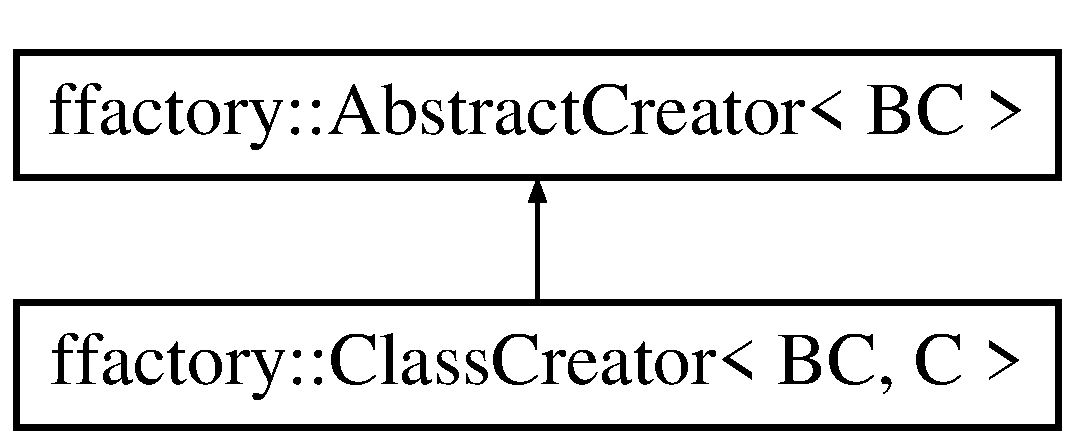
\includegraphics[height=2.000000cm]{classffactory_1_1_abstract_creator}
\end{center}
\end{figure}
\subsection*{Public Member Functions}
\begin{DoxyCompactItemize}
\item 
\hypertarget{classffactory_1_1_abstract_creator_ac9caa13d5fd6ed198700d3d9a6f2b92e}{virtual B\-C $\ast$ {\bfseries create} ()=0}\label{classffactory_1_1_abstract_creator_ac9caa13d5fd6ed198700d3d9a6f2b92e}

\end{DoxyCompactItemize}


\subsection{Detailed Description}
\subsubsection*{template$<$class B\-C$>$class ffactory\-::\-Abstract\-Creator$<$ B\-C $>$}

Abstract class-\/creator class 

The documentation for this class was generated from the following file\-:\begin{DoxyCompactItemize}
\item 
src/utils/patterns/Abstract\-Factory.\-h\end{DoxyCompactItemize}

\hypertarget{classffactory_1_1_abstract_factory}{\section{ffactory\-:\-:Abstract\-Factory$<$ B\-C $>$ Class Template Reference}
\label{classffactory_1_1_abstract_factory}\index{ffactory\-::\-Abstract\-Factory$<$ B\-C $>$@{ffactory\-::\-Abstract\-Factory$<$ B\-C $>$}}
}


{\ttfamily \#include $<$Abstract\-Factory.\-h$>$}

Inheritance diagram for ffactory\-:\-:Abstract\-Factory$<$ B\-C $>$\-:\begin{figure}[H]
\begin{center}
\leavevmode
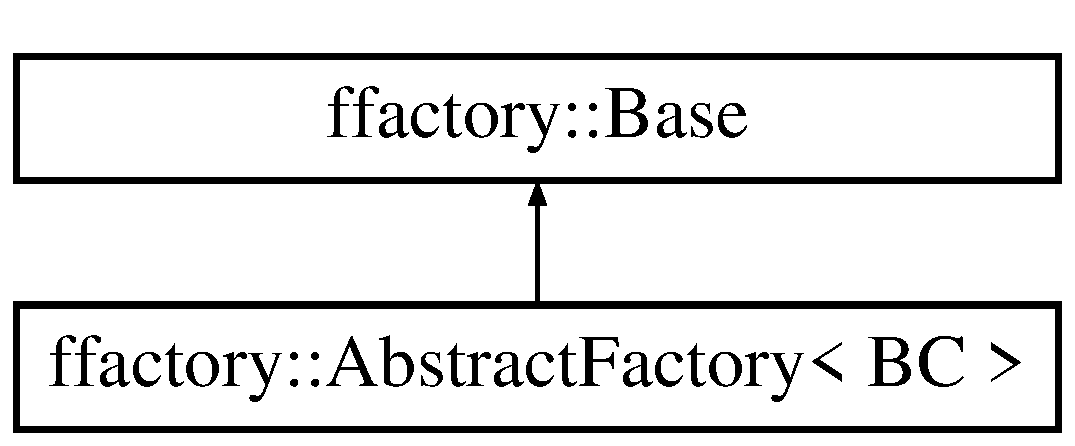
\includegraphics[height=2.000000cm]{classffactory_1_1_abstract_factory}
\end{center}
\end{figure}
\subsection*{Public Member Functions}
\begin{DoxyCompactItemize}
\item 
\hypertarget{classffactory_1_1_abstract_factory_a8223dea004ca4e4f78389729e886c4f4}{{\footnotesize template$<$class C $>$ }\\void {\bfseries add} (const std\-::string \&id)}\label{classffactory_1_1_abstract_factory_a8223dea004ca4e4f78389729e886c4f4}

\item 
B\-C $\ast$ \hyperlink{classffactory_1_1_abstract_factory_a822566f16b8bb4894f4930941b461ae8}{create} (const std\-::string \&id)
\item 
std\-::unique\-\_\-ptr$<$ B\-C $>$ \hyperlink{classffactory_1_1_abstract_factory_a50805631d6ed2790482d693b4388fe76}{create\-Unique} (const std\-::string \&id)
\item 
virtual void \hyperlink{classffactory_1_1_abstract_factory_acc3b114aecc19f8b4de596dba5bc7786}{Register} ()=0
\item 
std\-::string \hyperlink{classffactory_1_1_abstract_factory_ac34466fa6bbf769504437c90ae7b1a90}{list} ()
\end{DoxyCompactItemize}


\subsection{Detailed Description}
\subsubsection*{template$<$typename B\-C$>$class ffactory\-::\-Abstract\-Factory$<$ B\-C $>$}

Abstract factory pattern class for objects of base class B\-C 

\subsection{Member Function Documentation}
\hypertarget{classffactory_1_1_abstract_factory_a822566f16b8bb4894f4930941b461ae8}{\index{ffactory\-::\-Abstract\-Factory@{ffactory\-::\-Abstract\-Factory}!create@{create}}
\index{create@{create}!ffactory::AbstractFactory@{ffactory\-::\-Abstract\-Factory}}
\subsubsection[{create}]{\setlength{\rightskip}{0pt plus 5cm}template$<$typename B\-C$>$ B\-C$\ast$ {\bf ffactory\-::\-Abstract\-Factory}$<$ B\-C $>$\-::create (
\begin{DoxyParamCaption}
\item[{const std\-::string \&}]{id}
\end{DoxyParamCaption}
)\hspace{0.3cm}{\ttfamily [inline]}}}\label{classffactory_1_1_abstract_factory_a822566f16b8bb4894f4930941b461ae8}
Raw unsafe function to make class instance 
\begin{DoxyParams}{Parameters}
{\em id} & -\/ key of class \\
\hline
\end{DoxyParams}
\begin{DoxyReturn}{Returns}

\end{DoxyReturn}
\hypertarget{classffactory_1_1_abstract_factory_a50805631d6ed2790482d693b4388fe76}{\index{ffactory\-::\-Abstract\-Factory@{ffactory\-::\-Abstract\-Factory}!create\-Unique@{create\-Unique}}
\index{create\-Unique@{create\-Unique}!ffactory::AbstractFactory@{ffactory\-::\-Abstract\-Factory}}
\subsubsection[{create\-Unique}]{\setlength{\rightskip}{0pt plus 5cm}template$<$typename B\-C$>$ std\-::unique\-\_\-ptr$<$ B\-C $>$ {\bf ffactory\-::\-Abstract\-Factory}$<$ B\-C $>$\-::create\-Unique (
\begin{DoxyParamCaption}
\item[{const std\-::string \&}]{id}
\end{DoxyParamCaption}
)\hspace{0.3cm}{\ttfamily [inline]}}}\label{classffactory_1_1_abstract_factory_a50805631d6ed2790482d693b4388fe76}
Safe function to make class instance 
\begin{DoxyParams}{Parameters}
{\em id} & -\/ key of class \\
\hline
\end{DoxyParams}
\begin{DoxyReturn}{Returns}

\end{DoxyReturn}
\hypertarget{classffactory_1_1_abstract_factory_ac34466fa6bbf769504437c90ae7b1a90}{\index{ffactory\-::\-Abstract\-Factory@{ffactory\-::\-Abstract\-Factory}!list@{list}}
\index{list@{list}!ffactory::AbstractFactory@{ffactory\-::\-Abstract\-Factory}}
\subsubsection[{list}]{\setlength{\rightskip}{0pt plus 5cm}template$<$typename B\-C$>$ std\-::string {\bf ffactory\-::\-Abstract\-Factory}$<$ B\-C $>$\-::list (
\begin{DoxyParamCaption}
{}
\end{DoxyParamCaption}
)\hspace{0.3cm}{\ttfamily [inline]}}}\label{classffactory_1_1_abstract_factory_ac34466fa6bbf769504437c90ae7b1a90}
Generates string with key names of factory \begin{DoxyReturn}{Returns}

\end{DoxyReturn}
\hypertarget{classffactory_1_1_abstract_factory_acc3b114aecc19f8b4de596dba5bc7786}{\index{ffactory\-::\-Abstract\-Factory@{ffactory\-::\-Abstract\-Factory}!Register@{Register}}
\index{Register@{Register}!ffactory::AbstractFactory@{ffactory\-::\-Abstract\-Factory}}
\subsubsection[{Register}]{\setlength{\rightskip}{0pt plus 5cm}template$<$typename B\-C$>$ virtual void {\bf ffactory\-::\-Abstract\-Factory}$<$ B\-C $>$\-::Register (
\begin{DoxyParamCaption}
{}
\end{DoxyParamCaption}
)\hspace{0.3cm}{\ttfamily [pure virtual]}}}\label{classffactory_1_1_abstract_factory_acc3b114aecc19f8b4de596dba5bc7786}
Function must be called before using the class 

Implemented in \hyperlink{classffactory_1_1_file_reader_factory_a0f0b807dc1c92452b1cb97187ddf9f33}{ffactory\-::\-File\-Reader\-Factory}, \hyperlink{classffactory_1_1_accuracy_dependent_weight_factory_a67f333ed900e4b3ad41b3241a3eeb860}{ffactory\-::\-Accuracy\-Dependent\-Weight\-Factory}, and \hyperlink{classffactory_1_1_tree_node_factory_a99f98ac98e39bf3afc1e7d16ec2fec90}{ffactory\-::\-Tree\-Node\-Factory}.



The documentation for this class was generated from the following file\-:\begin{DoxyCompactItemize}
\item 
src/utils/patterns/Abstract\-Factory.\-h\end{DoxyCompactItemize}

\hypertarget{classffactory_1_1_accuracy_dependent_weight}{\section{ffactory\-:\-:Accuracy\-Dependent\-Weight Class Reference}
\label{classffactory_1_1_accuracy_dependent_weight}\index{ffactory\-::\-Accuracy\-Dependent\-Weight@{ffactory\-::\-Accuracy\-Dependent\-Weight}}
}


{\ttfamily \#include $<$Accuracy\-Dependent\-Weight.\-h$>$}

Inheritance diagram for ffactory\-:\-:Accuracy\-Dependent\-Weight\-:\begin{figure}[H]
\begin{center}
\leavevmode
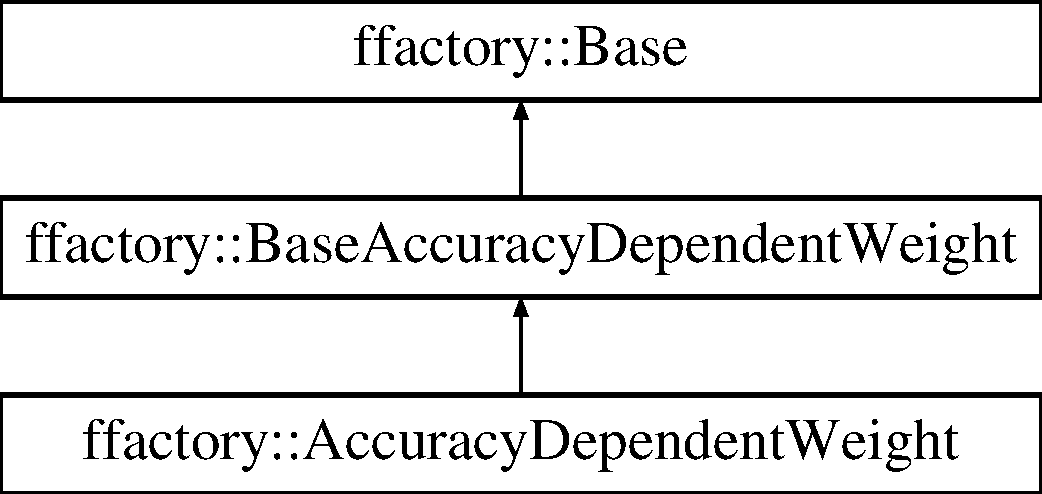
\includegraphics[height=3.000000cm]{classffactory_1_1_accuracy_dependent_weight}
\end{center}
\end{figure}
\subsection*{Public Member Functions}
\begin{DoxyCompactItemize}
\item 
virtual Data\-Vector\-Unique\-Ptr \hyperlink{classffactory_1_1_accuracy_dependent_weight_a7b912fc0846d557aea10d933501daade}{get\-Weights} (Data\-Vector $\ast$const error\-Vector)
\end{DoxyCompactItemize}


\subsection{Detailed Description}
\hyperlink{classffactory_1_1_base}{Base} classifier weighting function $ W_c(error) = \frac{1}{error+\delta} $ 

\subsection{Member Function Documentation}
\hypertarget{classffactory_1_1_accuracy_dependent_weight_a7b912fc0846d557aea10d933501daade}{\index{ffactory\-::\-Accuracy\-Dependent\-Weight@{ffactory\-::\-Accuracy\-Dependent\-Weight}!get\-Weights@{get\-Weights}}
\index{get\-Weights@{get\-Weights}!ffactory::AccuracyDependentWeight@{ffactory\-::\-Accuracy\-Dependent\-Weight}}
\subsubsection[{get\-Weights}]{\setlength{\rightskip}{0pt plus 5cm}Data\-Vector\-Unique\-Ptr ffactory\-::\-Accuracy\-Dependent\-Weight\-::get\-Weights (
\begin{DoxyParamCaption}
\item[{Data\-Vector $\ast$const}]{error\-Vector}
\end{DoxyParamCaption}
)\hspace{0.3cm}{\ttfamily [virtual]}}}\label{classffactory_1_1_accuracy_dependent_weight_a7b912fc0846d557aea10d933501daade}

\begin{DoxyParams}{Parameters}
{\em error\-Vector} & is a vector of errors of base classifiers (unnormalized) \\
\hline
\end{DoxyParams}
\begin{DoxyReturn}{Returns}
weights of base classifiers 
\end{DoxyReturn}


Implements \hyperlink{classffactory_1_1_base_accuracy_dependent_weight_a0baa145415e5e75b3b90c787c7e5a879}{ffactory\-::\-Base\-Accuracy\-Dependent\-Weight}.



The documentation for this class was generated from the following files\-:\begin{DoxyCompactItemize}
\item 
src/classifiers/ensemble/weighting/Accuracy\-Dependent\-Weight.\-h\item 
src/classifiers/ensemble/weighting/Accuracy\-Dependent\-Weight.\-cpp\end{DoxyCompactItemize}

\hypertarget{classffactory_1_1_accuracy_dependent_weight_factory}{\section{ffactory\-:\-:Accuracy\-Dependent\-Weight\-Factory Class Reference}
\label{classffactory_1_1_accuracy_dependent_weight_factory}\index{ffactory\-::\-Accuracy\-Dependent\-Weight\-Factory@{ffactory\-::\-Accuracy\-Dependent\-Weight\-Factory}}
}
Inheritance diagram for ffactory\-:\-:Accuracy\-Dependent\-Weight\-Factory\-:\begin{figure}[H]
\begin{center}
\leavevmode
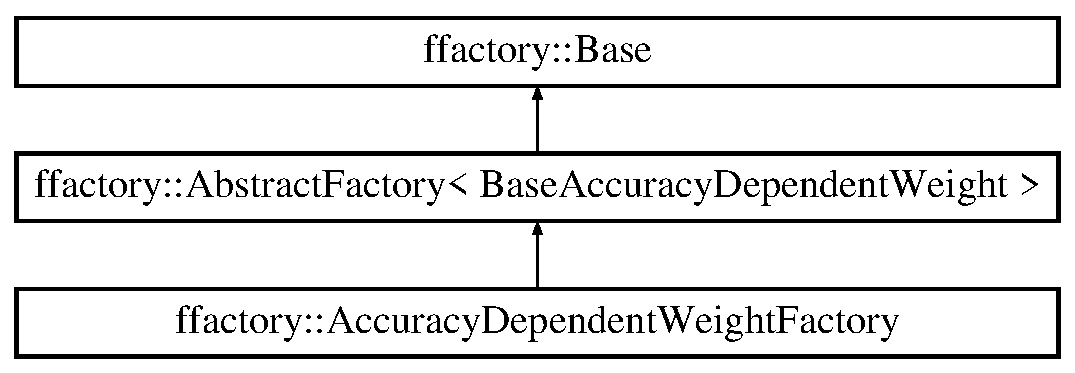
\includegraphics[height=3.000000cm]{classffactory_1_1_accuracy_dependent_weight_factory}
\end{center}
\end{figure}
\subsection*{Public Member Functions}
\begin{DoxyCompactItemize}
\item 
virtual void \hyperlink{classffactory_1_1_accuracy_dependent_weight_factory_a67f333ed900e4b3ad41b3241a3eeb860}{Register} ()
\end{DoxyCompactItemize}


\subsection{Member Function Documentation}
\hypertarget{classffactory_1_1_accuracy_dependent_weight_factory_a67f333ed900e4b3ad41b3241a3eeb860}{\index{ffactory\-::\-Accuracy\-Dependent\-Weight\-Factory@{ffactory\-::\-Accuracy\-Dependent\-Weight\-Factory}!Register@{Register}}
\index{Register@{Register}!ffactory::AccuracyDependentWeightFactory@{ffactory\-::\-Accuracy\-Dependent\-Weight\-Factory}}
\subsubsection[{Register}]{\setlength{\rightskip}{0pt plus 5cm}virtual void ffactory\-::\-Accuracy\-Dependent\-Weight\-Factory\-::\-Register (
\begin{DoxyParamCaption}
{}
\end{DoxyParamCaption}
)\hspace{0.3cm}{\ttfamily [inline]}, {\ttfamily [virtual]}}}\label{classffactory_1_1_accuracy_dependent_weight_factory_a67f333ed900e4b3ad41b3241a3eeb860}
Function must be called before using the class 

Implements \hyperlink{classffactory_1_1_abstract_factory_acc3b114aecc19f8b4de596dba5bc7786}{ffactory\-::\-Abstract\-Factory$<$ Base\-Accuracy\-Dependent\-Weight $>$}.



The documentation for this class was generated from the following file\-:\begin{DoxyCompactItemize}
\item 
src/classifiers/ensemble/weighting/Accuracy\-Dependent\-Weight\-Factory.\-h\end{DoxyCompactItemize}

\hypertarget{classffactory_1_1_a_r_f_f_file_reader}{\section{ffactory\-:\-:A\-R\-F\-F\-File\-Reader Class Reference}
\label{classffactory_1_1_a_r_f_f_file_reader}\index{ffactory\-::\-A\-R\-F\-F\-File\-Reader@{ffactory\-::\-A\-R\-F\-F\-File\-Reader}}
}
Inheritance diagram for ffactory\-:\-:A\-R\-F\-F\-File\-Reader\-:\begin{figure}[H]
\begin{center}
\leavevmode
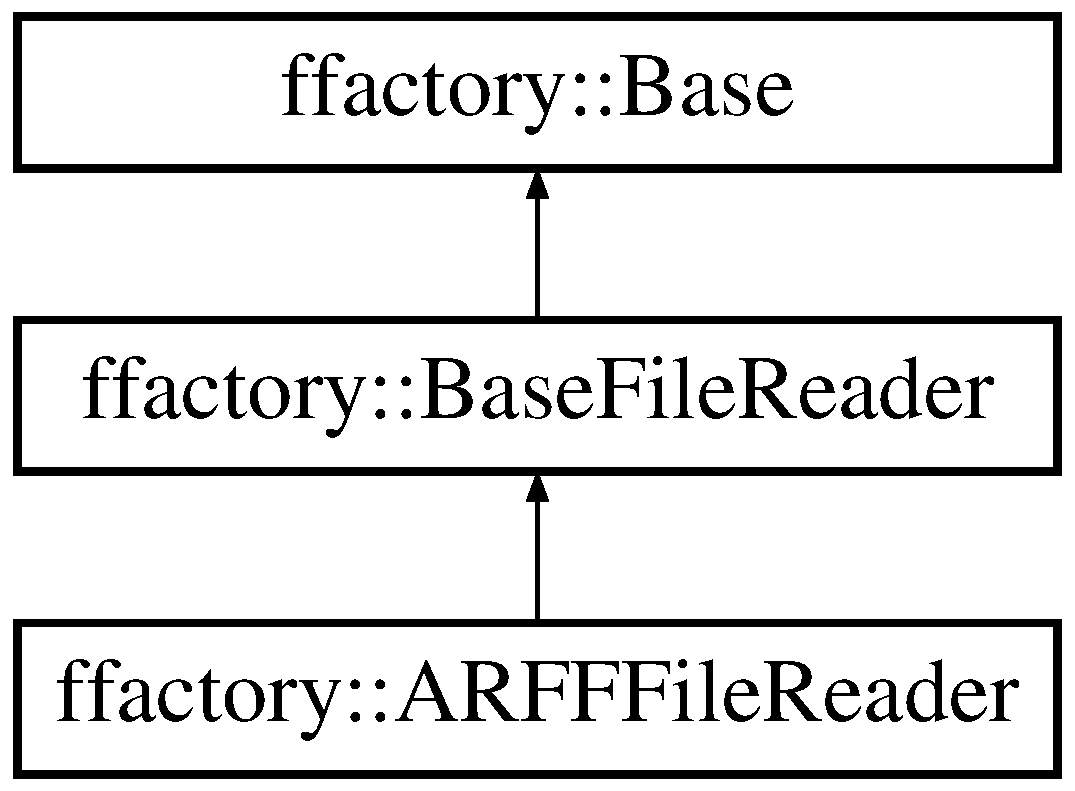
\includegraphics[height=3.000000cm]{classffactory_1_1_a_r_f_f_file_reader}
\end{center}
\end{figure}
\subsection*{Public Member Functions}
\begin{DoxyCompactItemize}
\item 
\hypertarget{classffactory_1_1_a_r_f_f_file_reader_ae3879c91a974667b3d64b1a2ad8a54d7}{{\bfseries A\-R\-F\-F\-File\-Reader} (std\-::string \-\_\-filename=\char`\"{}\char`\"{}, \hyperlink{classffactory_1_1_dataset}{Dataset} $\ast$\-\_\-dataset=N\-U\-L\-L)}\label{classffactory_1_1_a_r_f_f_file_reader_ae3879c91a974667b3d64b1a2ad8a54d7}

\item 
\hypertarget{classffactory_1_1_a_r_f_f_file_reader_a090c45ab33c278ee13f427157afb5188}{void {\bfseries read\-Header} (std\-::ifstream \&file, Index\-Type \&line\-Counter)}\label{classffactory_1_1_a_r_f_f_file_reader_a090c45ab33c278ee13f427157afb5188}

\item 
\hypertarget{classffactory_1_1_a_r_f_f_file_reader_af3c512a28af719e03fcbc3ba428fb1da}{void {\bfseries read\-Data} (std\-::ifstream \&file, Index\-Type \&line\-Counter)}\label{classffactory_1_1_a_r_f_f_file_reader_af3c512a28af719e03fcbc3ba428fb1da}

\item 
virtual void \hyperlink{classffactory_1_1_a_r_f_f_file_reader_ac2fe97202f44108f3379a787962c5721}{read} ()
\end{DoxyCompactItemize}
\subsection*{Additional Inherited Members}


\subsection{Member Function Documentation}
\hypertarget{classffactory_1_1_a_r_f_f_file_reader_ac2fe97202f44108f3379a787962c5721}{\index{ffactory\-::\-A\-R\-F\-F\-File\-Reader@{ffactory\-::\-A\-R\-F\-F\-File\-Reader}!read@{read}}
\index{read@{read}!ffactory::ARFFFileReader@{ffactory\-::\-A\-R\-F\-F\-File\-Reader}}
\subsubsection[{read}]{\setlength{\rightskip}{0pt plus 5cm}void ffactory\-::\-A\-R\-F\-F\-File\-Reader\-::read (
\begin{DoxyParamCaption}
{}
\end{DoxyParamCaption}
)\hspace{0.3cm}{\ttfamily [virtual]}}}\label{classffactory_1_1_a_r_f_f_file_reader_ac2fe97202f44108f3379a787962c5721}
Read file abstract method \begin{DoxyRefDesc}{Todo}
\item[\hyperlink{todo__todo000010}{Todo}]Num\-Classes should be set before add \end{DoxyRefDesc}


Implements \hyperlink{classffactory_1_1_base_file_reader_ab8683144beea50394ec833163d575615}{ffactory\-::\-Base\-File\-Reader}.



The documentation for this class was generated from the following files\-:\begin{DoxyCompactItemize}
\item 
src/data/file\-Formats/A\-R\-F\-F\-File\-Reader.\-h\item 
src/data/file\-Formats/A\-R\-F\-F\-File\-Reader.\-cpp\end{DoxyCompactItemize}

\hypertarget{classffactory_1_1_attribute}{\section{ffactory\-:\-:Attribute Class Reference}
\label{classffactory_1_1_attribute}\index{ffactory\-::\-Attribute@{ffactory\-::\-Attribute}}
}


{\ttfamily \#include $<$Attribute.\-h$>$}

Inheritance diagram for ffactory\-:\-:Attribute\-:\begin{figure}[H]
\begin{center}
\leavevmode
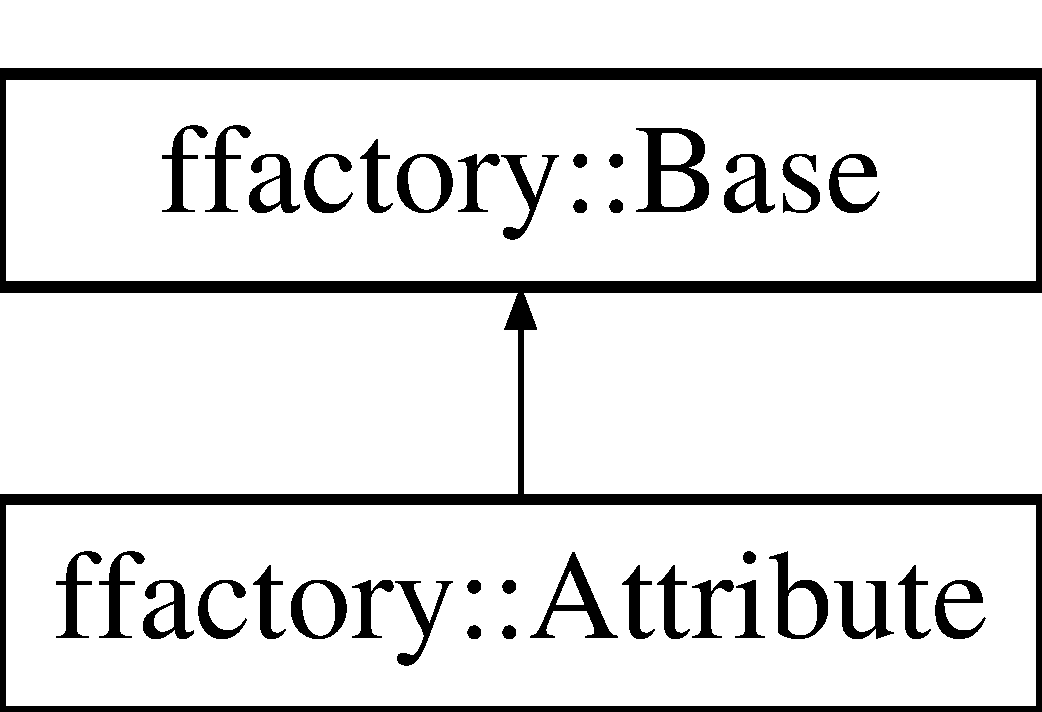
\includegraphics[height=2.000000cm]{classffactory_1_1_attribute}
\end{center}
\end{figure}
\subsection*{Public Member Functions}
\begin{DoxyCompactItemize}
\item 
\hypertarget{classffactory_1_1_attribute_a4b31d1e0fd0f4136b4f786999779c6bc}{Attribute\-Type {\bfseries get\-Type} () const }\label{classffactory_1_1_attribute_a4b31d1e0fd0f4136b4f786999779c6bc}

\item 
\hypertarget{classffactory_1_1_attribute_a0f55b7b1c41fce2cea4eb836db5ec733}{void {\bfseries set\-Type} (Attribute\-Type type)}\label{classffactory_1_1_attribute_a0f55b7b1c41fce2cea4eb836db5ec733}

\item 
\hypertarget{classffactory_1_1_attribute_a3353b447e5ee893561bc8d7568a854e8}{void {\bfseries set\-Categories} (String\-Vector $\ast$cat)}\label{classffactory_1_1_attribute_a3353b447e5ee893561bc8d7568a854e8}

\item 
\hypertarget{classffactory_1_1_attribute_a319721b6177179fd9a020ce5d17b9b88}{String\-Vector $\ast$ {\bfseries get\-Categories} ()}\label{classffactory_1_1_attribute_a319721b6177179fd9a020ce5d17b9b88}

\item 
\hypertarget{classffactory_1_1_attribute_a6f3cacacd898db9617dc7363585c801f}{Index\-Type {\bfseries get\-Num\-Categories} ()}\label{classffactory_1_1_attribute_a6f3cacacd898db9617dc7363585c801f}

\item 
\hypertarget{classffactory_1_1_attribute_aef23de3a7d441b6cd662fe48d67ab22a}{const std\-::string {\bfseries get\-Type\-Name} ()}\label{classffactory_1_1_attribute_aef23de3a7d441b6cd662fe48d67ab22a}

\item 
virtual std\-::string \hyperlink{classffactory_1_1_attribute_ad5494e94be89e79cefbbc40de865c970}{get\-Info} ()
\item 
\hypertarget{classffactory_1_1_attribute_aff54b418b06e8aa4f4830d88c496ed6b}{const char $\ast$ {\bfseries get\-Type\-String} ()}\label{classffactory_1_1_attribute_aff54b418b06e8aa4f4830d88c496ed6b}

\end{DoxyCompactItemize}


\subsection{Detailed Description}
\hyperlink{classffactory_1_1_attribute}{Attribute} type 

\subsection{Member Function Documentation}
\hypertarget{classffactory_1_1_attribute_ad5494e94be89e79cefbbc40de865c970}{\index{ffactory\-::\-Attribute@{ffactory\-::\-Attribute}!get\-Info@{get\-Info}}
\index{get\-Info@{get\-Info}!ffactory::Attribute@{ffactory\-::\-Attribute}}
\subsubsection[{get\-Info}]{\setlength{\rightskip}{0pt plus 5cm}virtual std\-::string ffactory\-::\-Attribute\-::get\-Info (
\begin{DoxyParamCaption}
{}
\end{DoxyParamCaption}
)\hspace{0.3cm}{\ttfamily [inline]}, {\ttfamily [virtual]}}}\label{classffactory_1_1_attribute_ad5494e94be89e79cefbbc40de865c970}
Generates information string \begin{DoxyReturn}{Returns}
std\-::string contains information about object 
\end{DoxyReturn}


Reimplemented from \hyperlink{classffactory_1_1_base_a061e6165abeadad3fac626253d14a0c6}{ffactory\-::\-Base}.



The documentation for this class was generated from the following file\-:\begin{DoxyCompactItemize}
\item 
src/data/Attribute.\-h\end{DoxyCompactItemize}

\hypertarget{classffactory_1_1_average_ensemble_aggregator}{\section{ffactory\-:\-:Average\-Ensemble\-Aggregator Class Reference}
\label{classffactory_1_1_average_ensemble_aggregator}\index{ffactory\-::\-Average\-Ensemble\-Aggregator@{ffactory\-::\-Average\-Ensemble\-Aggregator}}
}


{\ttfamily \#include $<$Average\-Ensemble\-Aggregator.\-h$>$}

Inheritance diagram for ffactory\-:\-:Average\-Ensemble\-Aggregator\-:\begin{figure}[H]
\begin{center}
\leavevmode
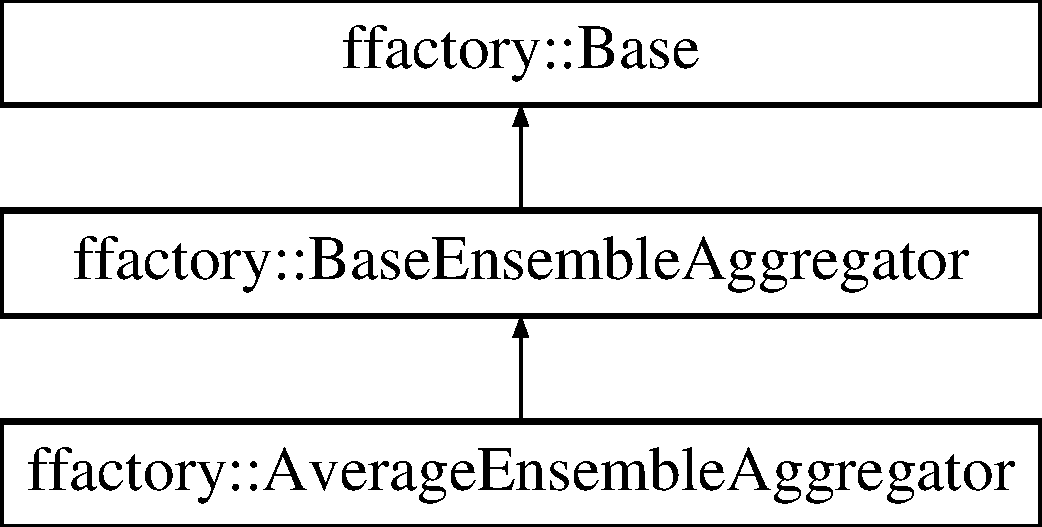
\includegraphics[height=3.000000cm]{classffactory_1_1_average_ensemble_aggregator}
\end{center}
\end{figure}
\subsection*{Public Member Functions}
\begin{DoxyCompactItemize}
\item 
\hypertarget{classffactory_1_1_average_ensemble_aggregator_a1f812408174d02496204067efa76b8d9}{void {\bfseries add\-Class\-Result\-Vector} (\hyperlink{classffactory_1_1_base_classifier}{Base\-Classifier} $\ast$c, Data\-Vector \&v)}\label{classffactory_1_1_average_ensemble_aggregator_a1f812408174d02496204067efa76b8d9}

\item 
virtual Data\-Vector\-Unique\-Ptr \hyperlink{classffactory_1_1_average_ensemble_aggregator_acfdd35393c0e5db156573a237a025f11}{aggregate} ()
\item 
\hypertarget{classffactory_1_1_average_ensemble_aggregator_a143fe19f5e807b6059b7d4bd25e29655}{virtual void {\bfseries set\-Num\-Classes} (unsigned int num\-Classes)}\label{classffactory_1_1_average_ensemble_aggregator_a143fe19f5e807b6059b7d4bd25e29655}

\end{DoxyCompactItemize}
\subsection*{Additional Inherited Members}


\subsection{Detailed Description}
Aggregate by averaging 

\subsection{Member Function Documentation}
\hypertarget{classffactory_1_1_average_ensemble_aggregator_acfdd35393c0e5db156573a237a025f11}{\index{ffactory\-::\-Average\-Ensemble\-Aggregator@{ffactory\-::\-Average\-Ensemble\-Aggregator}!aggregate@{aggregate}}
\index{aggregate@{aggregate}!ffactory::AverageEnsembleAggregator@{ffactory\-::\-Average\-Ensemble\-Aggregator}}
\subsubsection[{aggregate}]{\setlength{\rightskip}{0pt plus 5cm}virtual Data\-Vector\-Unique\-Ptr ffactory\-::\-Average\-Ensemble\-Aggregator\-::aggregate (
\begin{DoxyParamCaption}
{}
\end{DoxyParamCaption}
)\hspace{0.3cm}{\ttfamily [inline]}, {\ttfamily [virtual]}}}\label{classffactory_1_1_average_ensemble_aggregator_acfdd35393c0e5db156573a237a025f11}
Implementation of aggregation procedure here \begin{DoxyReturn}{Returns}

\end{DoxyReturn}


Implements \hyperlink{classffactory_1_1_base_ensemble_aggregator_a502352ca8f06449a0abc06f9381a6dc7}{ffactory\-::\-Base\-Ensemble\-Aggregator}.



The documentation for this class was generated from the following file\-:\begin{DoxyCompactItemize}
\item 
src/classifiers/ensemble/aggregator/Average\-Ensemble\-Aggregator.\-h\end{DoxyCompactItemize}

\hypertarget{classffactory_1_1_bagging_classifier}{\section{ffactory\-:\-:Bagging\-Classifier$<$ C $>$ Class Template Reference}
\label{classffactory_1_1_bagging_classifier}\index{ffactory\-::\-Bagging\-Classifier$<$ C $>$@{ffactory\-::\-Bagging\-Classifier$<$ C $>$}}
}


{\ttfamily \#include $<$Bagging\-Classifier.\-h$>$}

Inheritance diagram for ffactory\-:\-:Bagging\-Classifier$<$ C $>$\-:\begin{figure}[H]
\begin{center}
\leavevmode
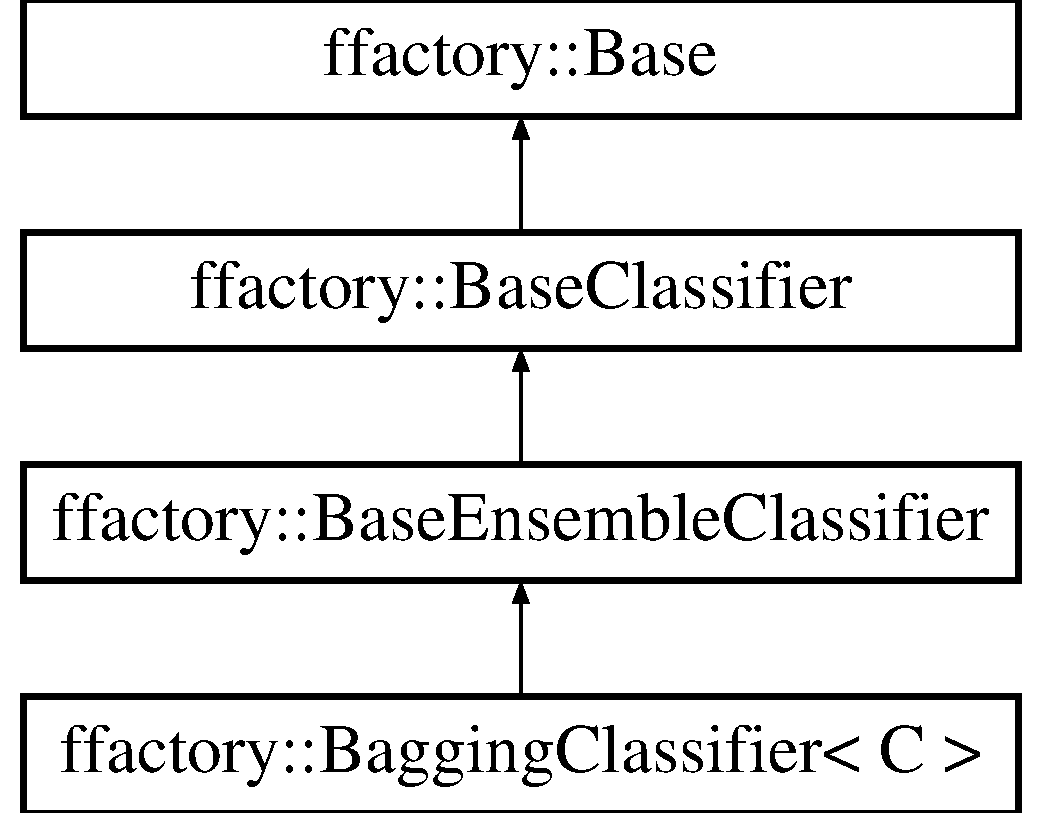
\includegraphics[height=4.000000cm]{classffactory_1_1_bagging_classifier}
\end{center}
\end{figure}
\subsection*{Public Member Functions}
\begin{DoxyCompactItemize}
\item 
\hypertarget{classffactory_1_1_bagging_classifier_ac8efae7493fe5fa73188c3104100faa7}{Index\-Vector $\ast$ {\bfseries get\-Ensemble\-Subset} (Index\-Type cidx)}\label{classffactory_1_1_bagging_classifier_ac8efae7493fe5fa73188c3104100faa7}

\item 
\hypertarget{classffactory_1_1_bagging_classifier_ac237abc196fba89c3e84b608957533dc}{Dataset\-Unique\-Ptr {\bfseries get\-O\-O\-B} (Index\-Type cidx)}\label{classffactory_1_1_bagging_classifier_ac237abc196fba89c3e84b608957533dc}

\item 
void \hyperlink{classffactory_1_1_bagging_classifier_ad5a99acbc8c7760ee7757317981b3c50}{train\-New\-Classifier} (\hyperlink{classffactory_1_1_dataset}{Dataset} $\ast$d)
\item 
virtual double \hyperlink{classffactory_1_1_bagging_classifier_ac99041bbde5f875cee90fcd7075c1f60}{train} (\hyperlink{classffactory_1_1_dataset}{Dataset} $\ast$d)
\item 
virtual Data\-Vector\-Unique\-Ptr \hyperlink{classffactory_1_1_bagging_classifier_ac6361c440269860eb1f7d4ff3d9ef4e3}{predict\-Class\-Prob} (\hyperlink{classffactory_1_1_sample}{Sample} \&sample)
\item 
\hypertarget{classffactory_1_1_bagging_classifier_afb7b8b7e668e366ab83bec48bf6ddbf7}{unsigned int {\bfseries get\-Classifiers\-Number} ()}\label{classffactory_1_1_bagging_classifier_afb7b8b7e668e366ab83bec48bf6ddbf7}

\item 
\hypertarget{classffactory_1_1_bagging_classifier_a91bfb18290a1a0f761fee9b237ed25ee}{unsigned int {\bfseries get\-Random\-Seed} () const }\label{classffactory_1_1_bagging_classifier_a91bfb18290a1a0f761fee9b237ed25ee}

\item 
\hypertarget{classffactory_1_1_bagging_classifier_a5f3fb156115904b433c397f76b15f02e}{void {\bfseries set\-Random\-Seed} (unsigned int random\-Seed)}\label{classffactory_1_1_bagging_classifier_a5f3fb156115904b433c397f76b15f02e}

\item 
\hypertarget{classffactory_1_1_bagging_classifier_a6e4505eaad83937f9e4b77ff5c6be302}{unsigned int {\bfseries get\-Train\-Subset\-Size} ()}\label{classffactory_1_1_bagging_classifier_a6e4505eaad83937f9e4b77ff5c6be302}

\item 
\hypertarget{classffactory_1_1_bagging_classifier_a9bf32f51bf6a4ab658c187e0a7907ae4}{void {\bfseries set\-Train\-Subset\-Size} (unsigned int train\-Subset\-Size)}\label{classffactory_1_1_bagging_classifier_a9bf32f51bf6a4ab658c187e0a7907ae4}

\end{DoxyCompactItemize}
\subsection*{Additional Inherited Members}


\subsection{Detailed Description}
\subsubsection*{template$<$typename C$>$class ffactory\-::\-Bagging\-Classifier$<$ C $>$}

\hyperlink{classffactory_1_1_base}{Base} class for all ensemble classifiers 

\subsection{Member Function Documentation}
\hypertarget{classffactory_1_1_bagging_classifier_ac6361c440269860eb1f7d4ff3d9ef4e3}{\index{ffactory\-::\-Bagging\-Classifier@{ffactory\-::\-Bagging\-Classifier}!predict\-Class\-Prob@{predict\-Class\-Prob}}
\index{predict\-Class\-Prob@{predict\-Class\-Prob}!ffactory::BaggingClassifier@{ffactory\-::\-Bagging\-Classifier}}
\subsubsection[{predict\-Class\-Prob}]{\setlength{\rightskip}{0pt plus 5cm}template$<$typename C $>$ virtual Data\-Vector\-Unique\-Ptr {\bf ffactory\-::\-Bagging\-Classifier}$<$ C $>$\-::predict\-Class\-Prob (
\begin{DoxyParamCaption}
\item[{{\bf Sample} \&}]{sample}
\end{DoxyParamCaption}
)\hspace{0.3cm}{\ttfamily [inline]}, {\ttfamily [virtual]}}}\label{classffactory_1_1_bagging_classifier_ac6361c440269860eb1f7d4ff3d9ef4e3}
Predict class probability of one sample 
\begin{DoxyParams}{Parameters}
{\em sample} & \\
\hline
\end{DoxyParams}
\begin{DoxyReturn}{Returns}
Index of class 
\end{DoxyReturn}
\hypertarget{classffactory_1_1_bagging_classifier_ac99041bbde5f875cee90fcd7075c1f60}{\index{ffactory\-::\-Bagging\-Classifier@{ffactory\-::\-Bagging\-Classifier}!train@{train}}
\index{train@{train}!ffactory::BaggingClassifier@{ffactory\-::\-Bagging\-Classifier}}
\subsubsection[{train}]{\setlength{\rightskip}{0pt plus 5cm}template$<$typename C $>$ virtual double {\bf ffactory\-::\-Bagging\-Classifier}$<$ C $>$\-::train (
\begin{DoxyParamCaption}
\item[{{\bf Dataset} $\ast$}]{d}
\end{DoxyParamCaption}
)\hspace{0.3cm}{\ttfamily [inline]}, {\ttfamily [virtual]}}}\label{classffactory_1_1_bagging_classifier_ac99041bbde5f875cee90fcd7075c1f60}
Train classifier on dataset {\itshape d} 
\begin{DoxyParams}{Parameters}
{\em d} & \\
\hline
\end{DoxyParams}
\begin{DoxyReturn}{Returns}
Value of specified error measure on dataset {\itshape d} 
\end{DoxyReturn}


Implements \hyperlink{classffactory_1_1_base_ensemble_classifier_a6ea804da2a71766b49372cbddb12cd50}{ffactory\-::\-Base\-Ensemble\-Classifier}.

\hypertarget{classffactory_1_1_bagging_classifier_ad5a99acbc8c7760ee7757317981b3c50}{\index{ffactory\-::\-Bagging\-Classifier@{ffactory\-::\-Bagging\-Classifier}!train\-New\-Classifier@{train\-New\-Classifier}}
\index{train\-New\-Classifier@{train\-New\-Classifier}!ffactory::BaggingClassifier@{ffactory\-::\-Bagging\-Classifier}}
\subsubsection[{train\-New\-Classifier}]{\setlength{\rightskip}{0pt plus 5cm}template$<$typename C $>$ void {\bf ffactory\-::\-Bagging\-Classifier}$<$ C $>$\-::train\-New\-Classifier (
\begin{DoxyParamCaption}
\item[{{\bf Dataset} $\ast$}]{d}
\end{DoxyParamCaption}
)\hspace{0.3cm}{\ttfamily [inline]}}}\label{classffactory_1_1_bagging_classifier_ad5a99acbc8c7760ee7757317981b3c50}
Generate new subset of train dataset and train new classifier on it. Result is pushed to vectors {\itshape ensemble} and {\itshape ensemble\-Subsets} 
\begin{DoxyParams}{Parameters}
{\em d} & \hyperlink{classffactory_1_1_dataset}{Dataset} \\
\hline
\end{DoxyParams}


The documentation for this class was generated from the following file\-:\begin{DoxyCompactItemize}
\item 
src/classifiers/ensemble/Bagging\-Classifier.\-h\end{DoxyCompactItemize}

\hypertarget{classffactory_1_1_balance_points_stoppage_criterion}{\section{ffactory\-:\-:Balance\-Points\-Stoppage\-Criterion Class Reference}
\label{classffactory_1_1_balance_points_stoppage_criterion}\index{ffactory\-::\-Balance\-Points\-Stoppage\-Criterion@{ffactory\-::\-Balance\-Points\-Stoppage\-Criterion}}
}
Inheritance diagram for ffactory\-:\-:Balance\-Points\-Stoppage\-Criterion\-:\begin{figure}[H]
\begin{center}
\leavevmode
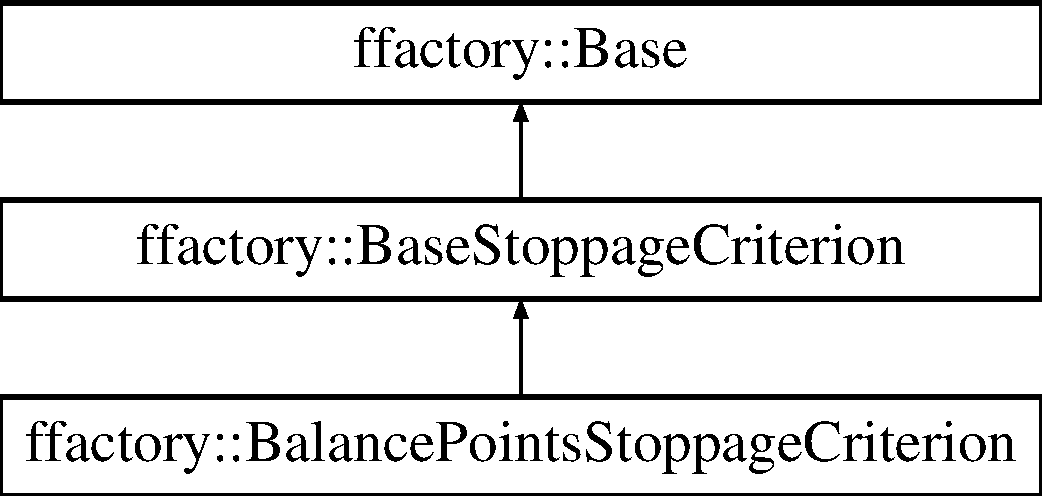
\includegraphics[height=3.000000cm]{classffactory_1_1_balance_points_stoppage_criterion}
\end{center}
\end{figure}
\subsection*{Public Member Functions}
\begin{DoxyCompactItemize}
\item 
\hypertarget{classffactory_1_1_balance_points_stoppage_criterion_ae1a3085d671d80623c9be4ef1a460381}{{\bfseries Balance\-Points\-Stoppage\-Criterion} (Index\-Type number, Index\-Type th, Data\-Type per)}\label{classffactory_1_1_balance_points_stoppage_criterion_ae1a3085d671d80623c9be4ef1a460381}

\item 
virtual bool \hyperlink{classffactory_1_1_balance_points_stoppage_criterion_ad27450524ea56f2b3925f56014c5ea7d}{Is\-Stoppage\-Needed} (\hyperlink{classffactory_1_1_base_tree_node}{Base\-Tree\-Node} $\ast$current\-Node, Data\-Vector \&class\-Prob\-Distr)
\item 
virtual std\-::string \hyperlink{classffactory_1_1_balance_points_stoppage_criterion_ae5414001f1c98a7fccf961a5015b3aa5}{get\-Info} ()
\end{DoxyCompactItemize}


\subsection{Member Function Documentation}
\hypertarget{classffactory_1_1_balance_points_stoppage_criterion_ae5414001f1c98a7fccf961a5015b3aa5}{\index{ffactory\-::\-Balance\-Points\-Stoppage\-Criterion@{ffactory\-::\-Balance\-Points\-Stoppage\-Criterion}!get\-Info@{get\-Info}}
\index{get\-Info@{get\-Info}!ffactory::BalancePointsStoppageCriterion@{ffactory\-::\-Balance\-Points\-Stoppage\-Criterion}}
\subsubsection[{get\-Info}]{\setlength{\rightskip}{0pt plus 5cm}virtual std\-::string ffactory\-::\-Balance\-Points\-Stoppage\-Criterion\-::get\-Info (
\begin{DoxyParamCaption}
{}
\end{DoxyParamCaption}
)\hspace{0.3cm}{\ttfamily [inline]}, {\ttfamily [virtual]}}}\label{classffactory_1_1_balance_points_stoppage_criterion_ae5414001f1c98a7fccf961a5015b3aa5}
Generates information string \begin{DoxyReturn}{Returns}
std\-::string contains information about object 
\end{DoxyReturn}


Reimplemented from \hyperlink{classffactory_1_1_base_stoppage_criterion_a0543f9c748cb8092e08314a8d2d40c79}{ffactory\-::\-Base\-Stoppage\-Criterion}.

\hypertarget{classffactory_1_1_balance_points_stoppage_criterion_ad27450524ea56f2b3925f56014c5ea7d}{\index{ffactory\-::\-Balance\-Points\-Stoppage\-Criterion@{ffactory\-::\-Balance\-Points\-Stoppage\-Criterion}!Is\-Stoppage\-Needed@{Is\-Stoppage\-Needed}}
\index{Is\-Stoppage\-Needed@{Is\-Stoppage\-Needed}!ffactory::BalancePointsStoppageCriterion@{ffactory\-::\-Balance\-Points\-Stoppage\-Criterion}}
\subsubsection[{Is\-Stoppage\-Needed}]{\setlength{\rightskip}{0pt plus 5cm}virtual bool ffactory\-::\-Balance\-Points\-Stoppage\-Criterion\-::\-Is\-Stoppage\-Needed (
\begin{DoxyParamCaption}
\item[{{\bf Base\-Tree\-Node} $\ast$}]{current\-Node, }
\item[{Data\-Vector \&}]{class\-Prob\-Distr}
\end{DoxyParamCaption}
)\hspace{0.3cm}{\ttfamily [inline]}, {\ttfamily [virtual]}}}\label{classffactory_1_1_balance_points_stoppage_criterion_ad27450524ea56f2b3925f56014c5ea7d}
Depth stoppage criterion 
\begin{DoxyParams}{Parameters}
{\em current\-Node} & \\
\hline
{\em class\-Prob\-Distr} & \\
\hline
\end{DoxyParams}
\begin{DoxyReturn}{Returns}

\end{DoxyReturn}


Implements \hyperlink{classffactory_1_1_base_stoppage_criterion_a47728f0c9b241133e228ea5956248241}{ffactory\-::\-Base\-Stoppage\-Criterion}.



The documentation for this class was generated from the following file\-:\begin{DoxyCompactItemize}
\item 
src/classifiers/trees/stoppage\-Criteria/balance\-Points\-Stoppage\-Criterion.\-h\end{DoxyCompactItemize}

\hypertarget{classffactory_1_1_base}{\section{ffactory\-:\-:Base Class Reference}
\label{classffactory_1_1_base}\index{ffactory\-::\-Base@{ffactory\-::\-Base}}
}


{\ttfamily \#include $<$Base.\-h$>$}

Inheritance diagram for ffactory\-:\-:Base\-:\begin{figure}[H]
\begin{center}
\leavevmode
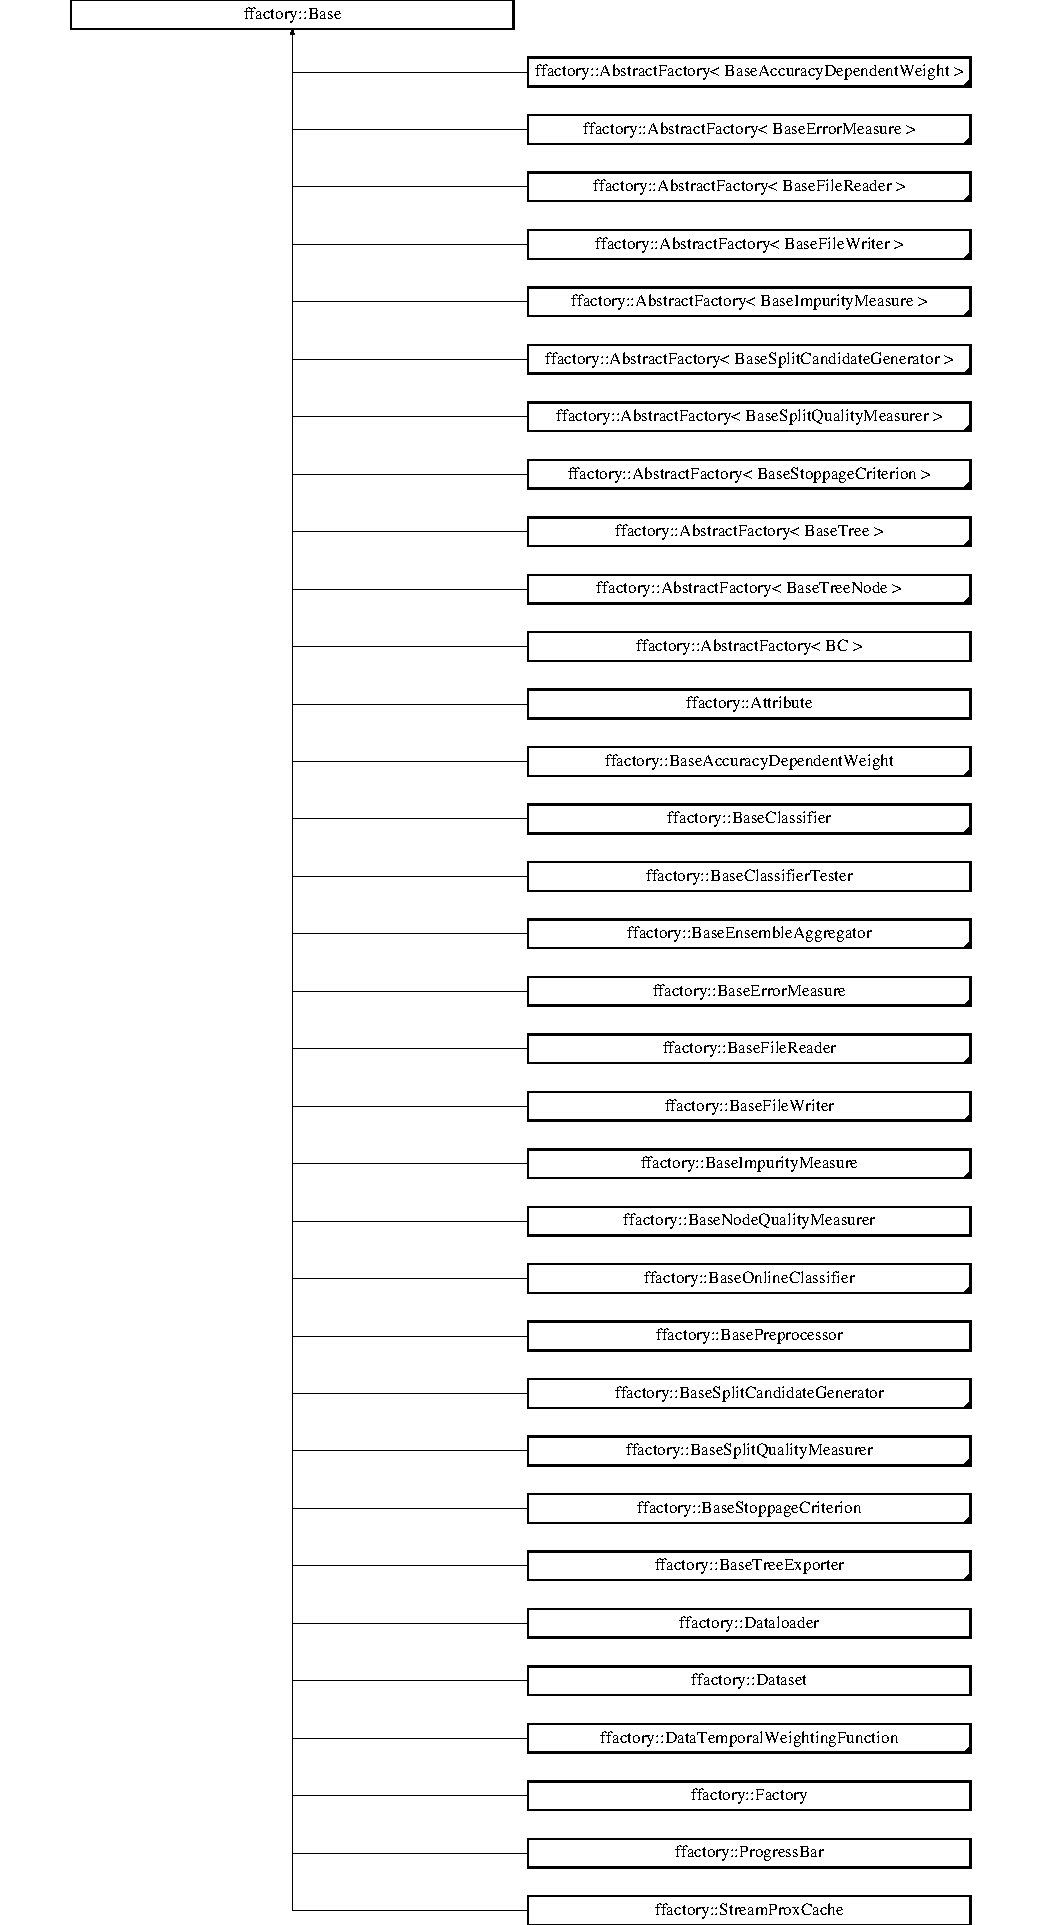
\includegraphics[height=12.000000cm]{classffactory_1_1_base}
\end{center}
\end{figure}
\subsection*{Public Member Functions}
\begin{DoxyCompactItemize}
\item 
\hypertarget{classffactory_1_1_base_a4330edb86dc9a45905cca6c56947566f}{std\-::string {\bfseries get\-Name} () const }\label{classffactory_1_1_base_a4330edb86dc9a45905cca6c56947566f}

\item 
\hypertarget{classffactory_1_1_base_a35832a4e794f5393df77d266cf073a03}{void {\bfseries set\-Name} (std\-::string name)}\label{classffactory_1_1_base_a35832a4e794f5393df77d266cf073a03}

\item 
virtual std\-::string \hyperlink{classffactory_1_1_base_a061e6165abeadad3fac626253d14a0c6}{get\-Info} ()
\end{DoxyCompactItemize}
\subsection*{Friends}
\begin{DoxyCompactItemize}
\item 
\hypertarget{classffactory_1_1_base_aae9c38e5df0e61027cc088958e6f0b76}{std\-::ostream \& {\bfseries operator$<$$<$} (std\-::ostream \&stream, \hyperlink{classffactory_1_1_base}{Base} \&b)}\label{classffactory_1_1_base_aae9c38e5df0e61027cc088958e6f0b76}

\end{DoxyCompactItemize}


\subsection{Detailed Description}
\hyperlink{classffactory_1_1_base}{Base} class for all Forest \hyperlink{classffactory_1_1_factory}{Factory} objects except small data containers like \hyperlink{classffactory_1_1_sample}{Sample} 

\subsection{Member Function Documentation}
\hypertarget{classffactory_1_1_base_a061e6165abeadad3fac626253d14a0c6}{\index{ffactory\-::\-Base@{ffactory\-::\-Base}!get\-Info@{get\-Info}}
\index{get\-Info@{get\-Info}!ffactory::Base@{ffactory\-::\-Base}}
\subsubsection[{get\-Info}]{\setlength{\rightskip}{0pt plus 5cm}virtual std\-::string ffactory\-::\-Base\-::get\-Info (
\begin{DoxyParamCaption}
{}
\end{DoxyParamCaption}
)\hspace{0.3cm}{\ttfamily [inline]}, {\ttfamily [virtual]}}}\label{classffactory_1_1_base_a061e6165abeadad3fac626253d14a0c6}
Generates information string \begin{DoxyReturn}{Returns}
std\-::string contains information about object 
\end{DoxyReturn}


Reimplemented in \hyperlink{classffactory_1_1_base_tree_a21d7faa1c68bb531522a73c36b10a95c}{ffactory\-::\-Base\-Tree}, \hyperlink{classffactory_1_1_dataset_a3017145c5f83813b81918aa0b2a9679b}{ffactory\-::\-Dataset}, \hyperlink{classffactory_1_1_random_split_candidate_generator_ab5ec1be9458ea7f7626f47bce9754bd6}{ffactory\-::\-Random\-Split\-Candidate\-Generator}, \hyperlink{classffactory_1_1_base_split_candidate_generator_a9247b20b96b60d227f3f3484e5614f39}{ffactory\-::\-Base\-Split\-Candidate\-Generator}, \hyperlink{classffactory_1_1_base_classifier_af6b0a89fd34ba70626104500d612d836}{ffactory\-::\-Base\-Classifier}, \hyperlink{classffactory_1_1_attribute_ad5494e94be89e79cefbbc40de865c970}{ffactory\-::\-Attribute}, \hyperlink{classffactory_1_1_decision_stump_af2c5492cfe13d297b11a7aa491695998}{ffactory\-::\-Decision\-Stump}, \hyperlink{classffactory_1_1_balance_points_stoppage_criterion_ae5414001f1c98a7fccf961a5015b3aa5}{ffactory\-::\-Balance\-Points\-Stoppage\-Criterion}, \hyperlink{classffactory_1_1_base_node_quality_measurer_a7d93ff368d8b2b439c0f7310213bf63f}{ffactory\-::\-Base\-Node\-Quality\-Measurer}, \hyperlink{classffactory_1_1_base_stoppage_criterion_a0543f9c748cb8092e08314a8d2d40c79}{ffactory\-::\-Base\-Stoppage\-Criterion}, \hyperlink{classffactory_1_1_base_split_quality_measurer_a0bd98e9b10ef01211e0839e9a6f22d26}{ffactory\-::\-Base\-Split\-Quality\-Measurer}, \hyperlink{classffactory_1_1_depth_stoppage_criterion_aeb81f88755a7dbae93a176ce8cee5624}{ffactory\-::\-Depth\-Stoppage\-Criterion}, \hyperlink{classffactory_1_1_points_number_stoppage_criterion_af8eaa4b922862c103528d9326115c74f}{ffactory\-::\-Points\-Number\-Stoppage\-Criterion}, \hyperlink{classffactory_1_1_simple_split_quality_measurer_a2d35a560f2ba91a6be600c8d42f3332e}{ffactory\-::\-Simple\-Split\-Quality\-Measurer}, \hyperlink{classffactory_1_1_empty_stoppage_criterion_a19181caac08aad7d05fcc07307c93c70}{ffactory\-::\-Empty\-Stoppage\-Criterion}, and \hyperlink{classffactory_1_1_base_online_tree_ad814d53893b7321f3384677b864ba2de}{ffactory\-::\-Base\-Online\-Tree}.



The documentation for this class was generated from the following file\-:\begin{DoxyCompactItemize}
\item 
src/Base.\-h\end{DoxyCompactItemize}

\hypertarget{classffactory_1_1_base_accuracy_dependent_weight}{\section{ffactory\-:\-:Base\-Accuracy\-Dependent\-Weight Class Reference}
\label{classffactory_1_1_base_accuracy_dependent_weight}\index{ffactory\-::\-Base\-Accuracy\-Dependent\-Weight@{ffactory\-::\-Base\-Accuracy\-Dependent\-Weight}}
}


{\ttfamily \#include $<$Base\-Accuracy\-Dependent\-Weight.\-h$>$}

Inheritance diagram for ffactory\-:\-:Base\-Accuracy\-Dependent\-Weight\-:\begin{figure}[H]
\begin{center}
\leavevmode
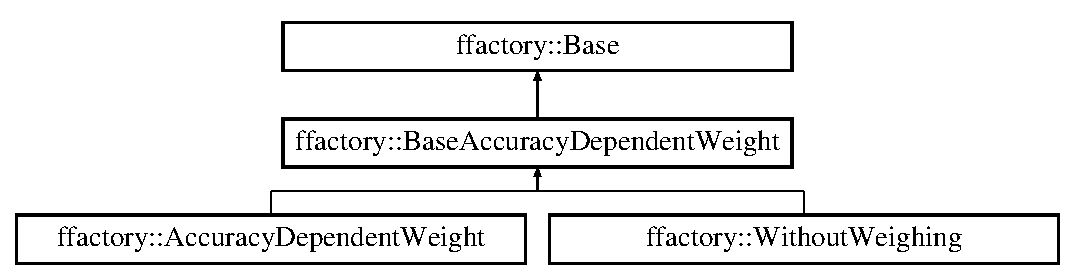
\includegraphics[height=3.000000cm]{classffactory_1_1_base_accuracy_dependent_weight}
\end{center}
\end{figure}
\subsection*{Public Member Functions}
\begin{DoxyCompactItemize}
\item 
virtual Data\-Vector\-Unique\-Ptr \hyperlink{classffactory_1_1_base_accuracy_dependent_weight_a0baa145415e5e75b3b90c787c7e5a879}{get\-Weights} (Data\-Vector $\ast$const error\-Vector)=0
\end{DoxyCompactItemize}


\subsection{Detailed Description}
Abstract class for base classifier weights computer. 

\subsection{Member Function Documentation}
\hypertarget{classffactory_1_1_base_accuracy_dependent_weight_a0baa145415e5e75b3b90c787c7e5a879}{\index{ffactory\-::\-Base\-Accuracy\-Dependent\-Weight@{ffactory\-::\-Base\-Accuracy\-Dependent\-Weight}!get\-Weights@{get\-Weights}}
\index{get\-Weights@{get\-Weights}!ffactory::BaseAccuracyDependentWeight@{ffactory\-::\-Base\-Accuracy\-Dependent\-Weight}}
\subsubsection[{get\-Weights}]{\setlength{\rightskip}{0pt plus 5cm}virtual Data\-Vector\-Unique\-Ptr ffactory\-::\-Base\-Accuracy\-Dependent\-Weight\-::get\-Weights (
\begin{DoxyParamCaption}
\item[{Data\-Vector $\ast$const}]{error\-Vector}
\end{DoxyParamCaption}
)\hspace{0.3cm}{\ttfamily [pure virtual]}}}\label{classffactory_1_1_base_accuracy_dependent_weight_a0baa145415e5e75b3b90c787c7e5a879}

\begin{DoxyParams}{Parameters}
{\em error\-Vector} & is a vector of errors of base classifiers (unnormalized) \\
\hline
\end{DoxyParams}
\begin{DoxyReturn}{Returns}
weights of base classifiers 
\end{DoxyReturn}


Implemented in \hyperlink{classffactory_1_1_accuracy_dependent_weight_a7b912fc0846d557aea10d933501daade}{ffactory\-::\-Accuracy\-Dependent\-Weight}, and \hyperlink{classffactory_1_1_without_weighing_a8c5dec3d0dd648e4f4816162ec9f3677}{ffactory\-::\-Without\-Weighing}.



The documentation for this class was generated from the following file\-:\begin{DoxyCompactItemize}
\item 
src/classifiers/ensemble/weighting/Base\-Accuracy\-Dependent\-Weight.\-h\end{DoxyCompactItemize}

\hypertarget{classffactory_1_1_base_classifier}{\section{ffactory\-:\-:Base\-Classifier Class Reference}
\label{classffactory_1_1_base_classifier}\index{ffactory\-::\-Base\-Classifier@{ffactory\-::\-Base\-Classifier}}
}


{\ttfamily \#include $<$Base\-Classifier.\-h$>$}

Inheritance diagram for ffactory\-:\-:Base\-Classifier\-:\begin{figure}[H]
\begin{center}
\leavevmode
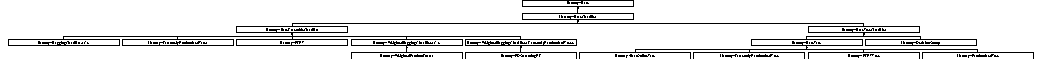
\includegraphics[height=0.789622cm]{classffactory_1_1_base_classifier}
\end{center}
\end{figure}
\subsection*{Public Member Functions}
\begin{DoxyCompactItemize}
\item 
virtual double \hyperlink{classffactory_1_1_base_classifier_a150000cb5cd9b2bb4380b47f33a462f2}{train} (\hyperlink{classffactory_1_1_dataset}{Dataset} $\ast$d)=0
\item 
virtual Data\-Vector\-Unique\-Ptr \hyperlink{classffactory_1_1_base_classifier_a6758932ce8f59eeffd0e66404a0332e4}{predict\-Class\-Prob} (\hyperlink{classffactory_1_1_sample}{Sample} $\ast$sample)=0
\item 
virtual \hyperlink{classffactory_1_1_prediction}{Prediction} \hyperlink{classffactory_1_1_base_classifier_ab8f15f99cd827ec7425e6ec0ce5c865d}{predict} (\hyperlink{classffactory_1_1_sample}{Sample} $\ast$sample)
\item 
virtual \hyperlink{classffactory_1_1_prediction}{Prediction} \hyperlink{classffactory_1_1_base_classifier_a769d4163c4785d27703b65954d4274c0}{predict} (\hyperlink{classffactory_1_1_dataset}{Dataset} \&d)
\item 
virtual double \hyperlink{classffactory_1_1_base_classifier_a08971f48a777aae6d23485b3bb469f6f}{test} (\hyperlink{classffactory_1_1_dataset}{Dataset} $\ast$d)
\item 
virtual std\-::string \hyperlink{classffactory_1_1_base_classifier_af6b0a89fd34ba70626104500d612d836}{get\-Info} ()
\item 
\hypertarget{classffactory_1_1_base_classifier_af93c7ccaf45c41c736566b2cefcda79f}{Index\-Type {\bfseries get\-Num\-Classes} () const }\label{classffactory_1_1_base_classifier_af93c7ccaf45c41c736566b2cefcda79f}

\item 
\hypertarget{classffactory_1_1_base_classifier_acc3e3fabc05d9ffca9c2845d66ae8325}{void {\bfseries set\-Num\-Classes} (Index\-Type num\-Classes)}\label{classffactory_1_1_base_classifier_acc3e3fabc05d9ffca9c2845d66ae8325}

\item 
\hypertarget{classffactory_1_1_base_classifier_afeacbc50664a260ae78691414fcb77bb}{Index\-Type {\bfseries get\-Num\-Features} () const }\label{classffactory_1_1_base_classifier_afeacbc50664a260ae78691414fcb77bb}

\item 
\hypertarget{classffactory_1_1_base_classifier_a13da1111aa19bcb20bc14718d7eb1544}{void {\bfseries set\-Num\-Features} (Index\-Type num\-Features)}\label{classffactory_1_1_base_classifier_a13da1111aa19bcb20bc14718d7eb1544}

\item 
\hypertarget{classffactory_1_1_base_classifier_a1d965abe43be8fc4e07bd6b69d67ba1d}{Index\-Type {\bfseries get\-Num\-Train\-Samples} () const }\label{classffactory_1_1_base_classifier_a1d965abe43be8fc4e07bd6b69d67ba1d}

\item 
\hypertarget{classffactory_1_1_base_classifier_a7afc4e7b030cd51444c6c31f192c368d}{void {\bfseries set\-Num\-Train\-Samples} (Index\-Type num\-Train\-Samples)}\label{classffactory_1_1_base_classifier_a7afc4e7b030cd51444c6c31f192c368d}

\item 
\hypertarget{classffactory_1_1_base_classifier_a6ba6914a0ff543fded2d0df1945d7e51}{bool {\bfseries is\-Verbose} () const }\label{classffactory_1_1_base_classifier_a6ba6914a0ff543fded2d0df1945d7e51}

\item 
\hypertarget{classffactory_1_1_base_classifier_a637e5d80d159e0749b15131358b02dc3}{void {\bfseries set\-Verbose} (bool verbose)}\label{classffactory_1_1_base_classifier_a637e5d80d159e0749b15131358b02dc3}

\item 
\hypertarget{classffactory_1_1_base_classifier_af37b1fd7f706c3eb41b53b6ca07288b7}{\hyperlink{classffactory_1_1_dataset}{Dataset} $\ast$ {\bfseries get\-Train\-Dataset} ()}\label{classffactory_1_1_base_classifier_af37b1fd7f706c3eb41b53b6ca07288b7}

\item 
\hypertarget{classffactory_1_1_base_classifier_a17ea29ce32addd94ea9c562a60a90288}{void {\bfseries set\-Train\-Dataset} (\hyperlink{classffactory_1_1_dataset}{Dataset} $\ast$train\-Dataset)}\label{classffactory_1_1_base_classifier_a17ea29ce32addd94ea9c562a60a90288}

\item 
\hypertarget{classffactory_1_1_base_classifier_aefd0240b6634ca6df4c85e53ef363e2f}{Index\-Vector \& {\bfseries get\-Train\-Indices} ()}\label{classffactory_1_1_base_classifier_aefd0240b6634ca6df4c85e53ef363e2f}

\item 
\hypertarget{classffactory_1_1_base_classifier_af918439bc7ec053abde1ddd9f460f71d}{void {\bfseries set\-Train\-Indices} (Index\-Vector \&train\-Indices)}\label{classffactory_1_1_base_classifier_af918439bc7ec053abde1ddd9f460f71d}

\item 
\hypertarget{classffactory_1_1_base_classifier_aa02807120d614d6a5f3bc84e4a334303}{\hyperlink{classffactory_1_1_base_error_measure}{Base\-Error\-Measure} $\ast$ {\bfseries get\-Error\-Measure} ()}\label{classffactory_1_1_base_classifier_aa02807120d614d6a5f3bc84e4a334303}

\item 
\hypertarget{classffactory_1_1_base_classifier_a6ba6f935bbf4d7a62cc34186024f0ab1}{void {\bfseries set\-Error\-Measure} (Base\-Error\-Measure\-Unique\-Ptr error\-Measure)}\label{classffactory_1_1_base_classifier_a6ba6f935bbf4d7a62cc34186024f0ab1}

\item 
\hypertarget{classffactory_1_1_base_classifier_a67e293cec5c93ff6c30ef94cce1a29ba}{void {\bfseries check} ()}\label{classffactory_1_1_base_classifier_a67e293cec5c93ff6c30ef94cce1a29ba}

\end{DoxyCompactItemize}


\subsection{Detailed Description}
Class with essential functions for all classification problems 

\subsection{Member Function Documentation}
\hypertarget{classffactory_1_1_base_classifier_af6b0a89fd34ba70626104500d612d836}{\index{ffactory\-::\-Base\-Classifier@{ffactory\-::\-Base\-Classifier}!get\-Info@{get\-Info}}
\index{get\-Info@{get\-Info}!ffactory::BaseClassifier@{ffactory\-::\-Base\-Classifier}}
\subsubsection[{get\-Info}]{\setlength{\rightskip}{0pt plus 5cm}virtual std\-::string ffactory\-::\-Base\-Classifier\-::get\-Info (
\begin{DoxyParamCaption}
{}
\end{DoxyParamCaption}
)\hspace{0.3cm}{\ttfamily [inline]}, {\ttfamily [virtual]}}}\label{classffactory_1_1_base_classifier_af6b0a89fd34ba70626104500d612d836}
Generates information string \begin{DoxyReturn}{Returns}
std\-::string contains information about object 
\end{DoxyReturn}


Reimplemented from \hyperlink{classffactory_1_1_base_a061e6165abeadad3fac626253d14a0c6}{ffactory\-::\-Base}.



Reimplemented in \hyperlink{classffactory_1_1_base_tree_a21d7faa1c68bb531522a73c36b10a95c}{ffactory\-::\-Base\-Tree}, \hyperlink{classffactory_1_1_decision_stump_af2c5492cfe13d297b11a7aa491695998}{ffactory\-::\-Decision\-Stump}, and \hyperlink{classffactory_1_1_base_online_tree_ad814d53893b7321f3384677b864ba2de}{ffactory\-::\-Base\-Online\-Tree}.

\hypertarget{classffactory_1_1_base_classifier_ab8f15f99cd827ec7425e6ec0ce5c865d}{\index{ffactory\-::\-Base\-Classifier@{ffactory\-::\-Base\-Classifier}!predict@{predict}}
\index{predict@{predict}!ffactory::BaseClassifier@{ffactory\-::\-Base\-Classifier}}
\subsubsection[{predict}]{\setlength{\rightskip}{0pt plus 5cm}virtual {\bf Prediction} ffactory\-::\-Base\-Classifier\-::predict (
\begin{DoxyParamCaption}
\item[{{\bf Sample} $\ast$}]{sample}
\end{DoxyParamCaption}
)\hspace{0.3cm}{\ttfamily [inline]}, {\ttfamily [virtual]}}}\label{classffactory_1_1_base_classifier_ab8f15f99cd827ec7425e6ec0ce5c865d}
Predict class of one sample 
\begin{DoxyParams}{Parameters}
{\em sample} & \\
\hline
\end{DoxyParams}
\begin{DoxyReturn}{Returns}
\hyperlink{classffactory_1_1_prediction}{Prediction} object 
\end{DoxyReturn}
\begin{DoxyRefDesc}{Todo}
\item[\hyperlink{todo__todo000001}{Todo}]Use M\-A\-C\-R\-O instead of this \end{DoxyRefDesc}
\hypertarget{classffactory_1_1_base_classifier_a769d4163c4785d27703b65954d4274c0}{\index{ffactory\-::\-Base\-Classifier@{ffactory\-::\-Base\-Classifier}!predict@{predict}}
\index{predict@{predict}!ffactory::BaseClassifier@{ffactory\-::\-Base\-Classifier}}
\subsubsection[{predict}]{\setlength{\rightskip}{0pt plus 5cm}virtual {\bf Prediction} ffactory\-::\-Base\-Classifier\-::predict (
\begin{DoxyParamCaption}
\item[{{\bf Dataset} \&}]{d}
\end{DoxyParamCaption}
)\hspace{0.3cm}{\ttfamily [inline]}, {\ttfamily [virtual]}}}\label{classffactory_1_1_base_classifier_a769d4163c4785d27703b65954d4274c0}
Predict class for dataset 
\begin{DoxyParams}{Parameters}
{\em d} & \\
\hline
\end{DoxyParams}
\begin{DoxyReturn}{Returns}
\hyperlink{classffactory_1_1_prediction}{Prediction} object 
\end{DoxyReturn}
\hypertarget{classffactory_1_1_base_classifier_a6758932ce8f59eeffd0e66404a0332e4}{\index{ffactory\-::\-Base\-Classifier@{ffactory\-::\-Base\-Classifier}!predict\-Class\-Prob@{predict\-Class\-Prob}}
\index{predict\-Class\-Prob@{predict\-Class\-Prob}!ffactory::BaseClassifier@{ffactory\-::\-Base\-Classifier}}
\subsubsection[{predict\-Class\-Prob}]{\setlength{\rightskip}{0pt plus 5cm}virtual Data\-Vector\-Unique\-Ptr ffactory\-::\-Base\-Classifier\-::predict\-Class\-Prob (
\begin{DoxyParamCaption}
\item[{{\bf Sample} $\ast$}]{sample}
\end{DoxyParamCaption}
)\hspace{0.3cm}{\ttfamily [pure virtual]}}}\label{classffactory_1_1_base_classifier_a6758932ce8f59eeffd0e66404a0332e4}
Predict class probability of one sample 
\begin{DoxyParams}{Parameters}
{\em sample} & \\
\hline
\end{DoxyParams}
\begin{DoxyReturn}{Returns}
Index of class 
\end{DoxyReturn}


Implemented in \hyperlink{classffactory_1_1_base_tree_a962907c4083f23175550bf82059d35f0}{ffactory\-::\-Base\-Tree}, \hyperlink{classffactory_1_1_p_e_r_t_a5a5c35207769f3027dce04b69843bcc9}{ffactory\-::\-P\-E\-R\-T}, \hyperlink{classffactory_1_1_extremely_randomized_trees_aed8da96894903e5c8ee7a87add67d78d}{ffactory\-::\-Extremely\-Randomized\-Trees}, \hyperlink{classffactory_1_1_weighted_bagging_classifier_ae9653ff238505bd33cca67ed4e20513c}{ffactory\-::\-Weighted\-Bagging\-Classifier$<$ C $>$}, \hyperlink{classffactory_1_1_weighted_bagging_classifier_ae9653ff238505bd33cca67ed4e20513c}{ffactory\-::\-Weighted\-Bagging\-Classifier$<$ Extremely\-Randomized\-Tree $>$}, \hyperlink{classffactory_1_1_p_d_streaming_r_f_a4a3fc1045d27d15c0a4209378ea7789b}{ffactory\-::\-P\-D\-Streaming\-R\-F}, and \hyperlink{classffactory_1_1_base_ensemble_classifier_ac6da7b47a25c7c6481d6476891085d16}{ffactory\-::\-Base\-Ensemble\-Classifier}.

\hypertarget{classffactory_1_1_base_classifier_a08971f48a777aae6d23485b3bb469f6f}{\index{ffactory\-::\-Base\-Classifier@{ffactory\-::\-Base\-Classifier}!test@{test}}
\index{test@{test}!ffactory::BaseClassifier@{ffactory\-::\-Base\-Classifier}}
\subsubsection[{test}]{\setlength{\rightskip}{0pt plus 5cm}virtual double ffactory\-::\-Base\-Classifier\-::test (
\begin{DoxyParamCaption}
\item[{{\bf Dataset} $\ast$}]{d}
\end{DoxyParamCaption}
)\hspace{0.3cm}{\ttfamily [inline]}, {\ttfamily [virtual]}}}\label{classffactory_1_1_base_classifier_a08971f48a777aae6d23485b3bb469f6f}
Test trained classifier on dataset {\itshape d} 
\begin{DoxyParams}{Parameters}
{\em d} & \\
\hline
\end{DoxyParams}
\begin{DoxyReturn}{Returns}
specified error measure value for {\itshape d} 
\end{DoxyReturn}
\hypertarget{classffactory_1_1_base_classifier_a150000cb5cd9b2bb4380b47f33a462f2}{\index{ffactory\-::\-Base\-Classifier@{ffactory\-::\-Base\-Classifier}!train@{train}}
\index{train@{train}!ffactory::BaseClassifier@{ffactory\-::\-Base\-Classifier}}
\subsubsection[{train}]{\setlength{\rightskip}{0pt plus 5cm}virtual double ffactory\-::\-Base\-Classifier\-::train (
\begin{DoxyParamCaption}
\item[{{\bf Dataset} $\ast$}]{d}
\end{DoxyParamCaption}
)\hspace{0.3cm}{\ttfamily [pure virtual]}}}\label{classffactory_1_1_base_classifier_a150000cb5cd9b2bb4380b47f33a462f2}
Train classifier on dataset {\itshape d} 
\begin{DoxyParams}{Parameters}
{\em d} & \\
\hline
\end{DoxyParams}
\begin{DoxyReturn}{Returns}
Value of specified error measure on dataset {\itshape d} 
\end{DoxyReturn}


Implemented in \hyperlink{classffactory_1_1_p_e_r_t_a7e8906ac8c355ab9832578d8acd41db0}{ffactory\-::\-P\-E\-R\-T}, \hyperlink{classffactory_1_1_extremely_randomized_trees_aa422b510fa91c27fb61eecbd5663cbd8}{ffactory\-::\-Extremely\-Randomized\-Trees}, \hyperlink{classffactory_1_1_base_tree_ad93e4fb475d3159a378b5148b127a58a}{ffactory\-::\-Base\-Tree}, \hyperlink{classffactory_1_1_weighted_bagging_classifier_a9c083e5508f58695c569dd2a4df50fd3}{ffactory\-::\-Weighted\-Bagging\-Classifier$<$ C $>$}, \hyperlink{classffactory_1_1_weighted_bagging_classifier_a9c083e5508f58695c569dd2a4df50fd3}{ffactory\-::\-Weighted\-Bagging\-Classifier$<$ Extremely\-Randomized\-Tree $>$}, \hyperlink{classffactory_1_1_bagging_classifier_ac99041bbde5f875cee90fcd7075c1f60}{ffactory\-::\-Bagging\-Classifier$<$ C $>$}, \hyperlink{classffactory_1_1_p_d_streaming_r_f_a711860e77360cb3fa8ff2a3160657997}{ffactory\-::\-P\-D\-Streaming\-R\-F}, and \hyperlink{classffactory_1_1_base_ensemble_classifier_a6ea804da2a71766b49372cbddb12cd50}{ffactory\-::\-Base\-Ensemble\-Classifier}.



The documentation for this class was generated from the following file\-:\begin{DoxyCompactItemize}
\item 
src/classifiers/Base\-Classifier.\-h\end{DoxyCompactItemize}

\hypertarget{classffactory_1_1_base_classifier_tester}{\section{ffactory\-:\-:Base\-Classifier\-Tester Class Reference}
\label{classffactory_1_1_base_classifier_tester}\index{ffactory\-::\-Base\-Classifier\-Tester@{ffactory\-::\-Base\-Classifier\-Tester}}
}
Inheritance diagram for ffactory\-:\-:Base\-Classifier\-Tester\-:\begin{figure}[H]
\begin{center}
\leavevmode
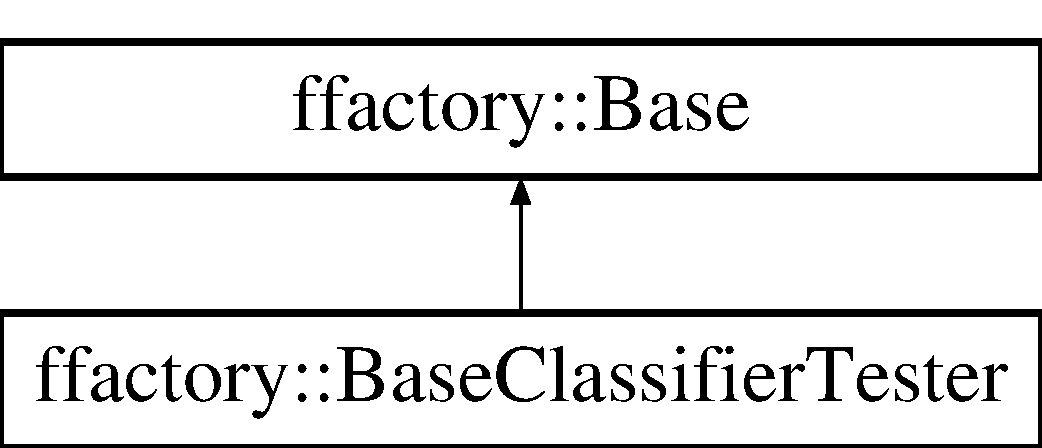
\includegraphics[height=2.000000cm]{classffactory_1_1_base_classifier_tester}
\end{center}
\end{figure}
\subsection*{Public Member Functions}
\begin{DoxyCompactItemize}
\item 
\hypertarget{classffactory_1_1_base_classifier_tester_af81d92ecb69257dd4353348d16955e26}{void {\bfseries add\-Parameter} (std\-::string name)}\label{classffactory_1_1_base_classifier_tester_af81d92ecb69257dd4353348d16955e26}

\item 
\hypertarget{classffactory_1_1_base_classifier_tester_ac4871c792a36124ead95c981985fb876}{void {\bfseries add\-Parameter\-Value} (std\-::string s, double val)}\label{classffactory_1_1_base_classifier_tester_ac4871c792a36124ead95c981985fb876}

\item 
\hypertarget{classffactory_1_1_base_classifier_tester_aa23052c083ad74bee350996fce2d972b}{\hyperlink{classffactory_1_1_parameter_set}{Parameter\-Set} $\ast$ {\bfseries get\-Parameter\-Set} (std\-::string name)}\label{classffactory_1_1_base_classifier_tester_aa23052c083ad74bee350996fce2d972b}

\item 
\hypertarget{classffactory_1_1_base_classifier_tester_a723c0872450cb17c51500522903ab22b}{double {\bfseries get\-Current} (const std\-::string name)}\label{classffactory_1_1_base_classifier_tester_a723c0872450cb17c51500522903ab22b}

\item 
\hypertarget{classffactory_1_1_base_classifier_tester_ab5c4b84416ecd74993c8a2511d8c1451}{std\-::string {\bfseries get\-Output} ()}\label{classffactory_1_1_base_classifier_tester_ab5c4b84416ecd74993c8a2511d8c1451}

\item 
\hypertarget{classffactory_1_1_base_classifier_tester_adc614e0d254d3a7ecc6fb6c7a3901f36}{void {\bfseries iterate} (const uint32\-\_\-t index)}\label{classffactory_1_1_base_classifier_tester_adc614e0d254d3a7ecc6fb6c7a3901f36}

\item 
\hypertarget{classffactory_1_1_base_classifier_tester_a4326b5a4aba9af63f3b59fdefe465522}{void {\bfseries run} ()}\label{classffactory_1_1_base_classifier_tester_a4326b5a4aba9af63f3b59fdefe465522}

\item 
\hypertarget{classffactory_1_1_base_classifier_tester_a10509e17be4fd4ad31adec31d80e5ac6}{virtual void {\bfseries setup} ()}\label{classffactory_1_1_base_classifier_tester_a10509e17be4fd4ad31adec31d80e5ac6}

\item 
\hypertarget{classffactory_1_1_base_classifier_tester_a8533abb37e38740e840064a22fb50a81}{virtual void {\bfseries iteration} ()}\label{classffactory_1_1_base_classifier_tester_a8533abb37e38740e840064a22fb50a81}

\item 
\hypertarget{classffactory_1_1_base_classifier_tester_a1d4e0885227b630d713d45bfb4388f1d}{virtual void {\bfseries tear\-Down} ()}\label{classffactory_1_1_base_classifier_tester_a1d4e0885227b630d713d45bfb4388f1d}

\end{DoxyCompactItemize}
\subsection*{Public Attributes}
\begin{DoxyCompactItemize}
\item 
\hypertarget{classffactory_1_1_base_classifier_tester_aa34c3f1803b71f8dbd932c74b37972ba}{Parameter\-Set\-Vector {\bfseries parameters}}\label{classffactory_1_1_base_classifier_tester_aa34c3f1803b71f8dbd932c74b37972ba}

\end{DoxyCompactItemize}
\subsection*{Protected Attributes}
\begin{DoxyCompactItemize}
\item 
\hypertarget{classffactory_1_1_base_classifier_tester_ac26b1322395902c088faceefe5c779c3}{std\-::stringstream {\bfseries ouput}}\label{classffactory_1_1_base_classifier_tester_ac26b1322395902c088faceefe5c779c3}

\end{DoxyCompactItemize}


The documentation for this class was generated from the following file\-:\begin{DoxyCompactItemize}
\item 
src/testers/Base\-Classifier\-Tester.\-h\end{DoxyCompactItemize}

\hypertarget{classffactory_1_1_base_ensemble_aggregator}{\section{ffactory\-:\-:Base\-Ensemble\-Aggregator Class Reference}
\label{classffactory_1_1_base_ensemble_aggregator}\index{ffactory\-::\-Base\-Ensemble\-Aggregator@{ffactory\-::\-Base\-Ensemble\-Aggregator}}
}


{\ttfamily \#include $<$Base\-Ensemble\-Aggregator.\-h$>$}

Inheritance diagram for ffactory\-:\-:Base\-Ensemble\-Aggregator\-:\begin{figure}[H]
\begin{center}
\leavevmode
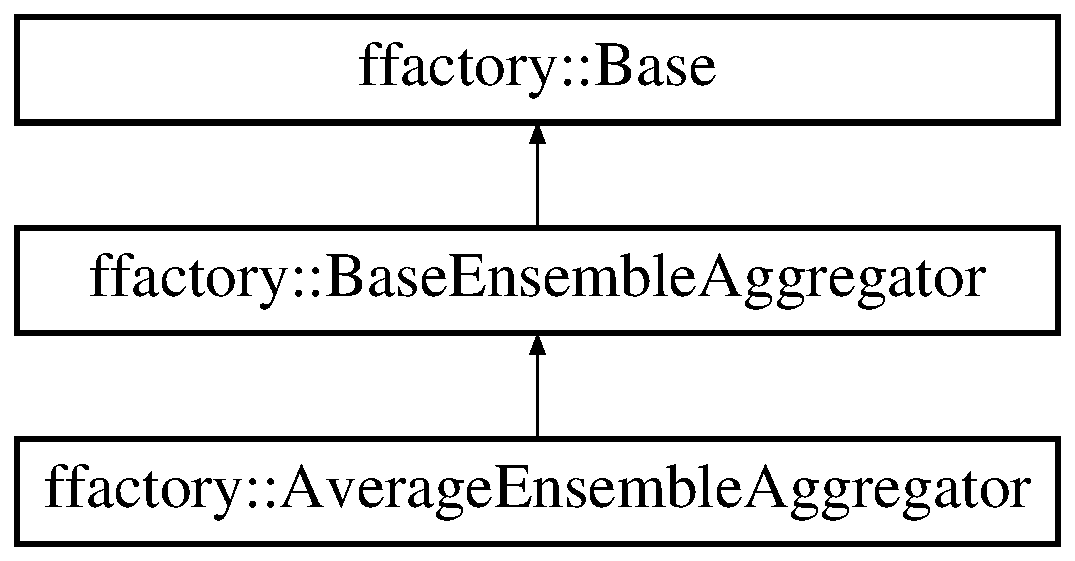
\includegraphics[height=3.000000cm]{classffactory_1_1_base_ensemble_aggregator}
\end{center}
\end{figure}
\subsection*{Public Member Functions}
\begin{DoxyCompactItemize}
\item 
void \hyperlink{classffactory_1_1_base_ensemble_aggregator_aa2dfb6aeef64ec84248b57966afc3fbd}{add\-Class\-Result\-Vector} (\hyperlink{classffactory_1_1_base_classifier}{Base\-Classifier} $\ast$c, Data\-Vector \&v)
\item 
\hypertarget{classffactory_1_1_base_ensemble_aggregator_a4de82c0fa84c84daeb6798bbcdbe274b}{void {\bfseries clear} ()}\label{classffactory_1_1_base_ensemble_aggregator_a4de82c0fa84c84daeb6798bbcdbe274b}

\item 
virtual Data\-Vector\-Unique\-Ptr \hyperlink{classffactory_1_1_base_ensemble_aggregator_a502352ca8f06449a0abc06f9381a6dc7}{aggregate} ()=0
\item 
\hypertarget{classffactory_1_1_base_ensemble_aggregator_a8a656e1521debd9cc3f10450d28457a4}{unsigned int {\bfseries get\-Num\-Classes} ()}\label{classffactory_1_1_base_ensemble_aggregator_a8a656e1521debd9cc3f10450d28457a4}

\item 
\hypertarget{classffactory_1_1_base_ensemble_aggregator_abc67844972315db87526c59be1b5f321}{virtual void {\bfseries set\-Num\-Classes} (unsigned int num\-Classes)}\label{classffactory_1_1_base_ensemble_aggregator_abc67844972315db87526c59be1b5f321}

\end{DoxyCompactItemize}
\subsection*{Protected Attributes}
\begin{DoxyCompactItemize}
\item 
\hypertarget{classffactory_1_1_base_ensemble_aggregator_a8d1913069526ac8a2306e138e94ae289}{Index\-Type {\bfseries num\-Classes}}\label{classffactory_1_1_base_ensemble_aggregator_a8d1913069526ac8a2306e138e94ae289}

\item 
\hypertarget{classffactory_1_1_base_ensemble_aggregator_af06791db8fb81e1d14e5f7c91f414e42}{std\-::vector$<$ Classifier\-Result\-Pair $>$ {\bfseries results}}\label{classffactory_1_1_base_ensemble_aggregator_af06791db8fb81e1d14e5f7c91f414e42}

\end{DoxyCompactItemize}


\subsection{Detailed Description}
\hyperlink{classffactory_1_1_base}{Base} class to aggregate results of base classifiers in ensemble 

\subsection{Member Function Documentation}
\hypertarget{classffactory_1_1_base_ensemble_aggregator_aa2dfb6aeef64ec84248b57966afc3fbd}{\index{ffactory\-::\-Base\-Ensemble\-Aggregator@{ffactory\-::\-Base\-Ensemble\-Aggregator}!add\-Class\-Result\-Vector@{add\-Class\-Result\-Vector}}
\index{add\-Class\-Result\-Vector@{add\-Class\-Result\-Vector}!ffactory::BaseEnsembleAggregator@{ffactory\-::\-Base\-Ensemble\-Aggregator}}
\subsubsection[{add\-Class\-Result\-Vector}]{\setlength{\rightskip}{0pt plus 5cm}void ffactory\-::\-Base\-Ensemble\-Aggregator\-::add\-Class\-Result\-Vector (
\begin{DoxyParamCaption}
\item[{{\bf Base\-Classifier} $\ast$}]{c, }
\item[{Data\-Vector \&}]{v}
\end{DoxyParamCaption}
)\hspace{0.3cm}{\ttfamily [inline]}}}\label{classffactory_1_1_base_ensemble_aggregator_aa2dfb6aeef64ec84248b57966afc3fbd}
Add classifier and its result 
\begin{DoxyParams}{Parameters}
{\em c} & Classifier \\
\hline
{\em v} & Resulting class probability \\
\hline
\end{DoxyParams}
\hypertarget{classffactory_1_1_base_ensemble_aggregator_a502352ca8f06449a0abc06f9381a6dc7}{\index{ffactory\-::\-Base\-Ensemble\-Aggregator@{ffactory\-::\-Base\-Ensemble\-Aggregator}!aggregate@{aggregate}}
\index{aggregate@{aggregate}!ffactory::BaseEnsembleAggregator@{ffactory\-::\-Base\-Ensemble\-Aggregator}}
\subsubsection[{aggregate}]{\setlength{\rightskip}{0pt plus 5cm}virtual Data\-Vector\-Unique\-Ptr ffactory\-::\-Base\-Ensemble\-Aggregator\-::aggregate (
\begin{DoxyParamCaption}
{}
\end{DoxyParamCaption}
)\hspace{0.3cm}{\ttfamily [pure virtual]}}}\label{classffactory_1_1_base_ensemble_aggregator_a502352ca8f06449a0abc06f9381a6dc7}
Implementation of aggregation procedure here \begin{DoxyReturn}{Returns}
Resulting ensemble class probability distribution 
\end{DoxyReturn}


Implemented in \hyperlink{classffactory_1_1_average_ensemble_aggregator_acfdd35393c0e5db156573a237a025f11}{ffactory\-::\-Average\-Ensemble\-Aggregator}.



The documentation for this class was generated from the following file\-:\begin{DoxyCompactItemize}
\item 
src/classifiers/ensemble/aggregator/Base\-Ensemble\-Aggregator.\-h\end{DoxyCompactItemize}

\hypertarget{classffactory_1_1_base_ensemble_classifier}{\section{ffactory\-:\-:Base\-Ensemble\-Classifier Class Reference}
\label{classffactory_1_1_base_ensemble_classifier}\index{ffactory\-::\-Base\-Ensemble\-Classifier@{ffactory\-::\-Base\-Ensemble\-Classifier}}
}


{\ttfamily \#include $<$Base\-Ensemble\-Classifier.\-h$>$}

Inheritance diagram for ffactory\-:\-:Base\-Ensemble\-Classifier\-:\begin{figure}[H]
\begin{center}
\leavevmode
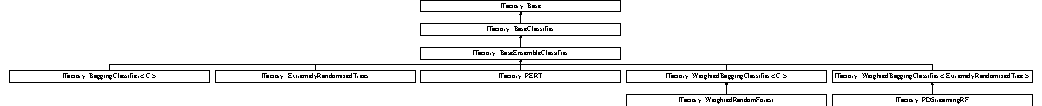
\includegraphics[height=1.421320cm]{classffactory_1_1_base_ensemble_classifier}
\end{center}
\end{figure}
\subsection*{Public Member Functions}
\begin{DoxyCompactItemize}
\item 
\hypertarget{classffactory_1_1_base_ensemble_classifier_afb635fc0bfe88a5100647c85afe373b3}{virtual void {\bfseries add\-Classifier} (Base\-Classifier\-Unique\-Ptr c)}\label{classffactory_1_1_base_ensemble_classifier_afb635fc0bfe88a5100647c85afe373b3}

\item 
\hypertarget{classffactory_1_1_base_ensemble_classifier_aea58a83aaec930aa021e67e704c251fc}{\hyperlink{classffactory_1_1_base_classifier}{Base\-Classifier} $\ast$ {\bfseries get\-Classifier} (Index\-Type idx)}\label{classffactory_1_1_base_ensemble_classifier_aea58a83aaec930aa021e67e704c251fc}

\item 
\hypertarget{classffactory_1_1_base_ensemble_classifier_ad026a89254a4c015efc0991015d85f01}{void {\bfseries remove\-Classifier} (Index\-Type idx)}\label{classffactory_1_1_base_ensemble_classifier_ad026a89254a4c015efc0991015d85f01}

\item 
virtual double \hyperlink{classffactory_1_1_base_ensemble_classifier_a6ea804da2a71766b49372cbddb12cd50}{train} (\hyperlink{classffactory_1_1_dataset}{Dataset} $\ast$d)=0
\item 
virtual Data\-Vector\-Unique\-Ptr \hyperlink{classffactory_1_1_base_ensemble_classifier_ac6da7b47a25c7c6481d6476891085d16}{predict\-Class\-Prob} (\hyperlink{classffactory_1_1_sample}{Sample} $\ast$sample)=0
\item 
std\-::vector\\*
$<$ Base\-Classifier\-Unique\-Ptr $>$ $\ast$ \hyperlink{classffactory_1_1_base_ensemble_classifier_a99dfac2d9fe4f6f380ded546070befb4}{get\-Ensemble} ()
\item 
\hypertarget{classffactory_1_1_base_ensemble_classifier_a9870bacad8acefb8014289bf99f82741}{\hyperlink{classffactory_1_1_base_ensemble_aggregator}{Base\-Ensemble\-Aggregator} $\ast$ {\bfseries get\-Aggregator} ()}\label{classffactory_1_1_base_ensemble_classifier_a9870bacad8acefb8014289bf99f82741}

\item 
\hypertarget{classffactory_1_1_base_ensemble_classifier_aa4a2fd1d18c05cbcc916657441bb63f1}{void {\bfseries set\-Aggregator} (Base\-Ensemble\-Aggregator\-Unique\-Ptr aggregator)}\label{classffactory_1_1_base_ensemble_classifier_aa4a2fd1d18c05cbcc916657441bb63f1}

\item 
\hypertarget{classffactory_1_1_base_ensemble_classifier_afd0663c86f1f0313bdac18cb93d07030}{Index\-Type {\bfseries get\-Num\-Classifiers\-To\-Train} ()}\label{classffactory_1_1_base_ensemble_classifier_afd0663c86f1f0313bdac18cb93d07030}

\item 
\hypertarget{classffactory_1_1_base_ensemble_classifier_a5f35f1379fa4e849ce5e5be7fb8ac0b7}{Index\-Type {\bfseries get\-Num\-Classifiers} ()}\label{classffactory_1_1_base_ensemble_classifier_a5f35f1379fa4e849ce5e5be7fb8ac0b7}

\item 
\hypertarget{classffactory_1_1_base_ensemble_classifier_a8523f3c50cb72816f0ac23bd2c1f6365}{void {\bfseries set\-Num\-Classifiers\-To\-Train} (Index\-Type num\-Classifiers\-To\-Train)}\label{classffactory_1_1_base_ensemble_classifier_a8523f3c50cb72816f0ac23bd2c1f6365}

\end{DoxyCompactItemize}
\subsection*{Protected Attributes}
\begin{DoxyCompactItemize}
\item 
\hypertarget{classffactory_1_1_base_ensemble_classifier_a8215e2bc0eefca0076058fc54b5c211c}{std\-::vector\\*
$<$ Base\-Classifier\-Unique\-Ptr $>$ {\bfseries ensemble}}\label{classffactory_1_1_base_ensemble_classifier_a8215e2bc0eefca0076058fc54b5c211c}

\end{DoxyCompactItemize}


\subsection{Detailed Description}
\hyperlink{classffactory_1_1_base}{Base} class for all ensemble classifiers 

\subsection{Member Function Documentation}
\hypertarget{classffactory_1_1_base_ensemble_classifier_a99dfac2d9fe4f6f380ded546070befb4}{\index{ffactory\-::\-Base\-Ensemble\-Classifier@{ffactory\-::\-Base\-Ensemble\-Classifier}!get\-Ensemble@{get\-Ensemble}}
\index{get\-Ensemble@{get\-Ensemble}!ffactory::BaseEnsembleClassifier@{ffactory\-::\-Base\-Ensemble\-Classifier}}
\subsubsection[{get\-Ensemble}]{\setlength{\rightskip}{0pt plus 5cm}std\-::vector$<$Base\-Classifier\-Unique\-Ptr$>$$\ast$ ffactory\-::\-Base\-Ensemble\-Classifier\-::get\-Ensemble (
\begin{DoxyParamCaption}
{}
\end{DoxyParamCaption}
)\hspace{0.3cm}{\ttfamily [inline]}}}\label{classffactory_1_1_base_ensemble_classifier_a99dfac2d9fe4f6f380ded546070befb4}
Predict class of one sample 
\begin{DoxyParams}{Parameters}
{\em sample} & \\
\hline
\end{DoxyParams}
\begin{DoxyReturn}{Returns}
\hyperlink{classffactory_1_1_prediction}{Prediction} Predict class for dataset 
\end{DoxyReturn}

\begin{DoxyParams}{Parameters}
{\em d} & \\
\hline
\end{DoxyParams}
\begin{DoxyReturn}{Returns}
Get pointer to ensemble vector 

std\-::vector$<$\-Base\-Classifier$\ast$$>$$\ast$ 
\end{DoxyReturn}
\hypertarget{classffactory_1_1_base_ensemble_classifier_ac6da7b47a25c7c6481d6476891085d16}{\index{ffactory\-::\-Base\-Ensemble\-Classifier@{ffactory\-::\-Base\-Ensemble\-Classifier}!predict\-Class\-Prob@{predict\-Class\-Prob}}
\index{predict\-Class\-Prob@{predict\-Class\-Prob}!ffactory::BaseEnsembleClassifier@{ffactory\-::\-Base\-Ensemble\-Classifier}}
\subsubsection[{predict\-Class\-Prob}]{\setlength{\rightskip}{0pt plus 5cm}virtual Data\-Vector\-Unique\-Ptr ffactory\-::\-Base\-Ensemble\-Classifier\-::predict\-Class\-Prob (
\begin{DoxyParamCaption}
\item[{{\bf Sample} $\ast$}]{sample}
\end{DoxyParamCaption}
)\hspace{0.3cm}{\ttfamily [pure virtual]}}}\label{classffactory_1_1_base_ensemble_classifier_ac6da7b47a25c7c6481d6476891085d16}
Predict class probability of one sample 
\begin{DoxyParams}{Parameters}
{\em sample} & \\
\hline
\end{DoxyParams}
\begin{DoxyReturn}{Returns}
Index of class 
\end{DoxyReturn}


Implements \hyperlink{classffactory_1_1_base_classifier_a6758932ce8f59eeffd0e66404a0332e4}{ffactory\-::\-Base\-Classifier}.



Implemented in \hyperlink{classffactory_1_1_p_e_r_t_a5a5c35207769f3027dce04b69843bcc9}{ffactory\-::\-P\-E\-R\-T}, \hyperlink{classffactory_1_1_extremely_randomized_trees_aed8da96894903e5c8ee7a87add67d78d}{ffactory\-::\-Extremely\-Randomized\-Trees}, \hyperlink{classffactory_1_1_weighted_bagging_classifier_ae9653ff238505bd33cca67ed4e20513c}{ffactory\-::\-Weighted\-Bagging\-Classifier$<$ C $>$}, \hyperlink{classffactory_1_1_weighted_bagging_classifier_ae9653ff238505bd33cca67ed4e20513c}{ffactory\-::\-Weighted\-Bagging\-Classifier$<$ Extremely\-Randomized\-Tree $>$}, and \hyperlink{classffactory_1_1_p_d_streaming_r_f_a4a3fc1045d27d15c0a4209378ea7789b}{ffactory\-::\-P\-D\-Streaming\-R\-F}.

\hypertarget{classffactory_1_1_base_ensemble_classifier_a6ea804da2a71766b49372cbddb12cd50}{\index{ffactory\-::\-Base\-Ensemble\-Classifier@{ffactory\-::\-Base\-Ensemble\-Classifier}!train@{train}}
\index{train@{train}!ffactory::BaseEnsembleClassifier@{ffactory\-::\-Base\-Ensemble\-Classifier}}
\subsubsection[{train}]{\setlength{\rightskip}{0pt plus 5cm}virtual double ffactory\-::\-Base\-Ensemble\-Classifier\-::train (
\begin{DoxyParamCaption}
\item[{{\bf Dataset} $\ast$}]{d}
\end{DoxyParamCaption}
)\hspace{0.3cm}{\ttfamily [pure virtual]}}}\label{classffactory_1_1_base_ensemble_classifier_a6ea804da2a71766b49372cbddb12cd50}
Train classifier on dataset {\itshape d} 
\begin{DoxyParams}{Parameters}
{\em d} & \\
\hline
\end{DoxyParams}
\begin{DoxyReturn}{Returns}
Value of specified error measure on dataset {\itshape d} 
\end{DoxyReturn}


Implements \hyperlink{classffactory_1_1_base_classifier_a150000cb5cd9b2bb4380b47f33a462f2}{ffactory\-::\-Base\-Classifier}.



Implemented in \hyperlink{classffactory_1_1_p_e_r_t_a7e8906ac8c355ab9832578d8acd41db0}{ffactory\-::\-P\-E\-R\-T}, \hyperlink{classffactory_1_1_extremely_randomized_trees_aa422b510fa91c27fb61eecbd5663cbd8}{ffactory\-::\-Extremely\-Randomized\-Trees}, \hyperlink{classffactory_1_1_weighted_bagging_classifier_a9c083e5508f58695c569dd2a4df50fd3}{ffactory\-::\-Weighted\-Bagging\-Classifier$<$ C $>$}, \hyperlink{classffactory_1_1_weighted_bagging_classifier_a9c083e5508f58695c569dd2a4df50fd3}{ffactory\-::\-Weighted\-Bagging\-Classifier$<$ Extremely\-Randomized\-Tree $>$}, \hyperlink{classffactory_1_1_bagging_classifier_ac99041bbde5f875cee90fcd7075c1f60}{ffactory\-::\-Bagging\-Classifier$<$ C $>$}, and \hyperlink{classffactory_1_1_p_d_streaming_r_f_a711860e77360cb3fa8ff2a3160657997}{ffactory\-::\-P\-D\-Streaming\-R\-F}.



The documentation for this class was generated from the following file\-:\begin{DoxyCompactItemize}
\item 
src/classifiers/ensemble/Base\-Ensemble\-Classifier.\-h\end{DoxyCompactItemize}

\hypertarget{classffactory_1_1_base_error_measure}{\section{ffactory\-:\-:Base\-Error\-Measure Class Reference}
\label{classffactory_1_1_base_error_measure}\index{ffactory\-::\-Base\-Error\-Measure@{ffactory\-::\-Base\-Error\-Measure}}
}


{\ttfamily \#include $<$base\-Error\-Measure.\-h$>$}

Inheritance diagram for ffactory\-:\-:Base\-Error\-Measure\-:\begin{figure}[H]
\begin{center}
\leavevmode
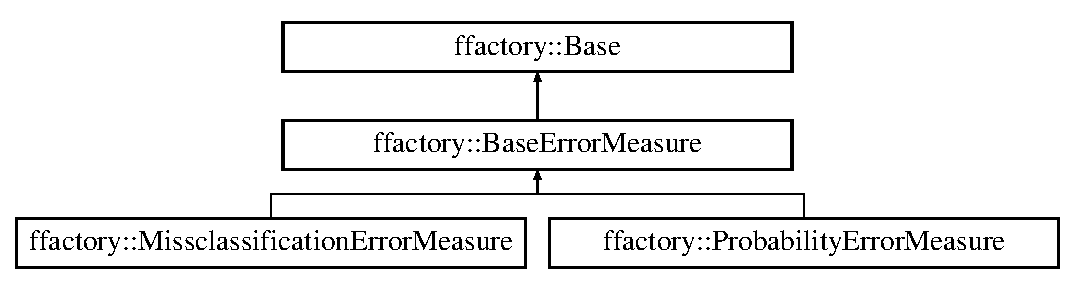
\includegraphics[height=3.000000cm]{classffactory_1_1_base_error_measure}
\end{center}
\end{figure}
\subsection*{Public Member Functions}
\begin{DoxyCompactItemize}
\item 
virtual double \hyperlink{classffactory_1_1_base_error_measure_a8eb4fef1cb479834c3fc1baac589d8b1}{get\-Error} (\hyperlink{classffactory_1_1_base_classifier}{Base\-Classifier} $\ast$c, \hyperlink{classffactory_1_1_sample}{Sample} \&s)=0
\item 
virtual double \hyperlink{classffactory_1_1_base_error_measure_a59333613908d58b1a5ff7208bd93d6fb}{get\-Error} (\hyperlink{classffactory_1_1_base_classifier}{Base\-Classifier} $\ast$c, \hyperlink{classffactory_1_1_dataset}{Dataset} $\ast$d)=0
\end{DoxyCompactItemize}


\subsection{Detailed Description}
Generic error measure class 

\subsection{Member Function Documentation}
\hypertarget{classffactory_1_1_base_error_measure_a8eb4fef1cb479834c3fc1baac589d8b1}{\index{ffactory\-::\-Base\-Error\-Measure@{ffactory\-::\-Base\-Error\-Measure}!get\-Error@{get\-Error}}
\index{get\-Error@{get\-Error}!ffactory::BaseErrorMeasure@{ffactory\-::\-Base\-Error\-Measure}}
\subsubsection[{get\-Error}]{\setlength{\rightskip}{0pt plus 5cm}virtual double ffactory\-::\-Base\-Error\-Measure\-::get\-Error (
\begin{DoxyParamCaption}
\item[{{\bf Base\-Classifier} $\ast$}]{c, }
\item[{{\bf Sample} \&}]{s}
\end{DoxyParamCaption}
)\hspace{0.3cm}{\ttfamily [pure virtual]}}}\label{classffactory_1_1_base_error_measure_a8eb4fef1cb479834c3fc1baac589d8b1}
Get error on current sample {\itshape s} 
\begin{DoxyParams}{Parameters}
{\em s} & \\
\hline
\end{DoxyParams}
\begin{DoxyReturn}{Returns}
error measure value 
\end{DoxyReturn}


Implemented in \hyperlink{classffactory_1_1_missclassification_error_measure_adedf3d4ccccf1dd24995d9e5d109afd3}{ffactory\-::\-Missclassification\-Error\-Measure}, and \hyperlink{classffactory_1_1_probability_error_measure_abfc0dd59747fd479663e9167c8510157}{ffactory\-::\-Probability\-Error\-Measure}.

\hypertarget{classffactory_1_1_base_error_measure_a59333613908d58b1a5ff7208bd93d6fb}{\index{ffactory\-::\-Base\-Error\-Measure@{ffactory\-::\-Base\-Error\-Measure}!get\-Error@{get\-Error}}
\index{get\-Error@{get\-Error}!ffactory::BaseErrorMeasure@{ffactory\-::\-Base\-Error\-Measure}}
\subsubsection[{get\-Error}]{\setlength{\rightskip}{0pt plus 5cm}virtual double ffactory\-::\-Base\-Error\-Measure\-::get\-Error (
\begin{DoxyParamCaption}
\item[{{\bf Base\-Classifier} $\ast$}]{c, }
\item[{{\bf Dataset} $\ast$}]{d}
\end{DoxyParamCaption}
)\hspace{0.3cm}{\ttfamily [pure virtual]}}}\label{classffactory_1_1_base_error_measure_a59333613908d58b1a5ff7208bd93d6fb}
Get error on entire dataset {\itshape d} 
\begin{DoxyParams}{Parameters}
{\em d} & \\
\hline
\end{DoxyParams}
\begin{DoxyReturn}{Returns}
error measure value 
\end{DoxyReturn}


Implemented in \hyperlink{classffactory_1_1_missclassification_error_measure_a962d88274011caaba227e7c7f6ce3bdf}{ffactory\-::\-Missclassification\-Error\-Measure}, and \hyperlink{classffactory_1_1_probability_error_measure_ac633b58b1e3be6feafb3b9fdd7fd1388}{ffactory\-::\-Probability\-Error\-Measure}.



The documentation for this class was generated from the following file\-:\begin{DoxyCompactItemize}
\item 
src/classifiers/error\-Measures/base\-Error\-Measure.\-h\end{DoxyCompactItemize}

\hypertarget{classffactory_1_1_base_file_reader}{\section{ffactory\-:\-:Base\-File\-Reader Class Reference}
\label{classffactory_1_1_base_file_reader}\index{ffactory\-::\-Base\-File\-Reader@{ffactory\-::\-Base\-File\-Reader}}
}


{\ttfamily \#include $<$Base\-File\-Reader.\-h$>$}

Inheritance diagram for ffactory\-:\-:Base\-File\-Reader\-:\begin{figure}[H]
\begin{center}
\leavevmode
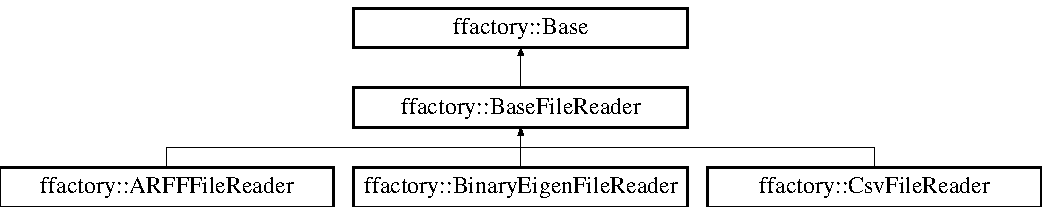
\includegraphics[height=2.786070cm]{classffactory_1_1_base_file_reader}
\end{center}
\end{figure}
\subsection*{Public Member Functions}
\begin{DoxyCompactItemize}
\item 
\hypertarget{classffactory_1_1_base_file_reader_a8d6a6ae99b1c1e5425e56fc90176e018}{{\bfseries Base\-File\-Reader} (std\-::string \-\_\-filename=\char`\"{}\char`\"{}, \hyperlink{classffactory_1_1_dataset}{Dataset} $\ast$\-\_\-dataset=N\-U\-L\-L)}\label{classffactory_1_1_base_file_reader_a8d6a6ae99b1c1e5425e56fc90176e018}

\item 
virtual void \hyperlink{classffactory_1_1_base_file_reader_ab8683144beea50394ec833163d575615}{read} ()=0
\item 
\hypertarget{classffactory_1_1_base_file_reader_a99ed2cb12be72b43273501146fc29163}{const std\-::string \& {\bfseries get\-Filename} () const }\label{classffactory_1_1_base_file_reader_a99ed2cb12be72b43273501146fc29163}

\item 
\hypertarget{classffactory_1_1_base_file_reader_a18d352a589ce02c9ab61793eb0a3e5a9}{void {\bfseries set\-Filename} (const std\-::string \&filename)}\label{classffactory_1_1_base_file_reader_a18d352a589ce02c9ab61793eb0a3e5a9}

\item 
\hypertarget{classffactory_1_1_base_file_reader_a3be5e024b10a4cc818e5c91c6c560262}{\hyperlink{classffactory_1_1_dataset}{Dataset} $\ast$ {\bfseries get\-Dataset} ()}\label{classffactory_1_1_base_file_reader_a3be5e024b10a4cc818e5c91c6c560262}

\item 
\hypertarget{classffactory_1_1_base_file_reader_a9b232c85c50435272cd73512ab67723e}{void {\bfseries set\-Dataset} (\hyperlink{classffactory_1_1_dataset}{Dataset} $\ast$dataset)}\label{classffactory_1_1_base_file_reader_a9b232c85c50435272cd73512ab67723e}

\item 
\hypertarget{classffactory_1_1_base_file_reader_accd449482bd147dda3aa63393e100d3e}{bool {\bfseries is\-Verbose} () const }\label{classffactory_1_1_base_file_reader_accd449482bd147dda3aa63393e100d3e}

\item 
\hypertarget{classffactory_1_1_base_file_reader_a543b5cae0d6a5503a09e857c5f06ca5e}{void {\bfseries set\-Verbose} (bool verbose)}\label{classffactory_1_1_base_file_reader_a543b5cae0d6a5503a09e857c5f06ca5e}

\end{DoxyCompactItemize}
\subsection*{Protected Attributes}
\begin{DoxyCompactItemize}
\item 
\hypertarget{classffactory_1_1_base_file_reader_ae5927a2027c87679275ebbe871699d1a}{bool {\bfseries verbose}}\label{classffactory_1_1_base_file_reader_ae5927a2027c87679275ebbe871699d1a}

\end{DoxyCompactItemize}


\subsection{Detailed Description}
Abstract class to provide interface to read many file formats datasets 

\subsection{Member Function Documentation}
\hypertarget{classffactory_1_1_base_file_reader_ab8683144beea50394ec833163d575615}{\index{ffactory\-::\-Base\-File\-Reader@{ffactory\-::\-Base\-File\-Reader}!read@{read}}
\index{read@{read}!ffactory::BaseFileReader@{ffactory\-::\-Base\-File\-Reader}}
\subsubsection[{read}]{\setlength{\rightskip}{0pt plus 5cm}virtual void ffactory\-::\-Base\-File\-Reader\-::read (
\begin{DoxyParamCaption}
{}
\end{DoxyParamCaption}
)\hspace{0.3cm}{\ttfamily [pure virtual]}}}\label{classffactory_1_1_base_file_reader_ab8683144beea50394ec833163d575615}
Read file abstract method 

Implemented in \hyperlink{classffactory_1_1_csv_file_reader_a82882543777400ac3779a89b986a5e98}{ffactory\-::\-Csv\-File\-Reader}, \hyperlink{classffactory_1_1_a_r_f_f_file_reader_ac2fe97202f44108f3379a787962c5721}{ffactory\-::\-A\-R\-F\-F\-File\-Reader}, and \hyperlink{classffactory_1_1_binary_eigen_file_reader_ab56d0d075f40f5a659b30f66f84811a4}{ffactory\-::\-Binary\-Eigen\-File\-Reader}.



The documentation for this class was generated from the following file\-:\begin{DoxyCompactItemize}
\item 
src/data/file\-Formats/Base\-File\-Reader.\-h\end{DoxyCompactItemize}

\hypertarget{classffactory_1_1_base_file_writer}{\section{ffactory\-:\-:Base\-File\-Writer Class Reference}
\label{classffactory_1_1_base_file_writer}\index{ffactory\-::\-Base\-File\-Writer@{ffactory\-::\-Base\-File\-Writer}}
}
Inheritance diagram for ffactory\-:\-:Base\-File\-Writer\-:\begin{figure}[H]
\begin{center}
\leavevmode
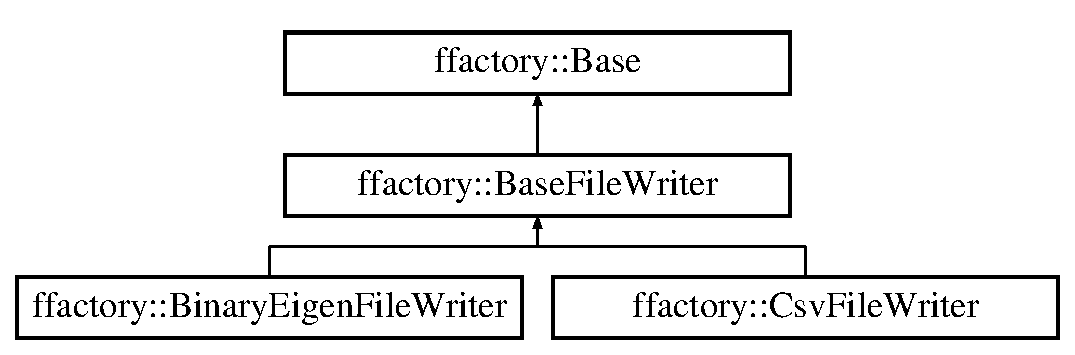
\includegraphics[height=3.000000cm]{classffactory_1_1_base_file_writer}
\end{center}
\end{figure}
\subsection*{Public Member Functions}
\begin{DoxyCompactItemize}
\item 
\hypertarget{classffactory_1_1_base_file_writer_a7abb233f705afbab3d6489df2510af52}{{\bfseries Base\-File\-Writer} (std\-::string \-\_\-filename=\char`\"{}\char`\"{}, \hyperlink{classffactory_1_1_dataset}{Dataset} $\ast$\-\_\-dataset=N\-U\-L\-L)}\label{classffactory_1_1_base_file_writer_a7abb233f705afbab3d6489df2510af52}

\item 
virtual void \hyperlink{classffactory_1_1_base_file_writer_a0674ebc35d7448fe40abead0057eb572}{write} ()=0
\item 
\hypertarget{classffactory_1_1_base_file_writer_a3f7621e653029b7674b84017e4eef869}{const std\-::string \& {\bfseries get\-Filename} () const }\label{classffactory_1_1_base_file_writer_a3f7621e653029b7674b84017e4eef869}

\item 
\hypertarget{classffactory_1_1_base_file_writer_addfae383869d69f91dc733511ce909e9}{void {\bfseries set\-Filename} (const std\-::string \&filename)}\label{classffactory_1_1_base_file_writer_addfae383869d69f91dc733511ce909e9}

\item 
\hypertarget{classffactory_1_1_base_file_writer_aaad3fee6d59733f098cac6dca2c64909}{\hyperlink{classffactory_1_1_dataset}{Dataset} $\ast$ {\bfseries get\-Dataset} ()}\label{classffactory_1_1_base_file_writer_aaad3fee6d59733f098cac6dca2c64909}

\item 
\hypertarget{classffactory_1_1_base_file_writer_ae86a7535ddf3fb98b21783bde855fea1}{void {\bfseries set\-Dataset} (\hyperlink{classffactory_1_1_dataset}{Dataset} $\ast$dataset)}\label{classffactory_1_1_base_file_writer_ae86a7535ddf3fb98b21783bde855fea1}

\item 
\hypertarget{classffactory_1_1_base_file_writer_a3db9b3039917a7c42774d51e8611ae23}{bool {\bfseries is\-Verbose} () const }\label{classffactory_1_1_base_file_writer_a3db9b3039917a7c42774d51e8611ae23}

\item 
\hypertarget{classffactory_1_1_base_file_writer_a23974bf4188af26cfc5bb67d57522f2d}{void {\bfseries set\-Verbose} (bool verbose)}\label{classffactory_1_1_base_file_writer_a23974bf4188af26cfc5bb67d57522f2d}

\end{DoxyCompactItemize}
\subsection*{Protected Attributes}
\begin{DoxyCompactItemize}
\item 
\hypertarget{classffactory_1_1_base_file_writer_a55596315454a104afc9da209c259ccb9}{bool {\bfseries verbose}}\label{classffactory_1_1_base_file_writer_a55596315454a104afc9da209c259ccb9}

\end{DoxyCompactItemize}


\subsection{Member Function Documentation}
\hypertarget{classffactory_1_1_base_file_writer_a0674ebc35d7448fe40abead0057eb572}{\index{ffactory\-::\-Base\-File\-Writer@{ffactory\-::\-Base\-File\-Writer}!write@{write}}
\index{write@{write}!ffactory::BaseFileWriter@{ffactory\-::\-Base\-File\-Writer}}
\subsubsection[{write}]{\setlength{\rightskip}{0pt plus 5cm}virtual void ffactory\-::\-Base\-File\-Writer\-::write (
\begin{DoxyParamCaption}
{}
\end{DoxyParamCaption}
)\hspace{0.3cm}{\ttfamily [pure virtual]}}}\label{classffactory_1_1_base_file_writer_a0674ebc35d7448fe40abead0057eb572}
Write file abstract method 

Implemented in \hyperlink{classffactory_1_1_binary_eigen_file_writer_a3c9cad431a2149b12e3842223b1e8b19}{ffactory\-::\-Binary\-Eigen\-File\-Writer}, and \hyperlink{classffactory_1_1_csv_file_writer_adf8696c5785a68b4a04e2d6f56b047b7}{ffactory\-::\-Csv\-File\-Writer}.



The documentation for this class was generated from the following file\-:\begin{DoxyCompactItemize}
\item 
src/data/file\-Formats/Base\-File\-Writer.\-h\end{DoxyCompactItemize}

\hypertarget{classffactory_1_1_base_impurity_measure}{\section{ffactory\-:\-:Base\-Impurity\-Measure Class Reference}
\label{classffactory_1_1_base_impurity_measure}\index{ffactory\-::\-Base\-Impurity\-Measure@{ffactory\-::\-Base\-Impurity\-Measure}}
}
Inheritance diagram for ffactory\-:\-:Base\-Impurity\-Measure\-:\begin{figure}[H]
\begin{center}
\leavevmode
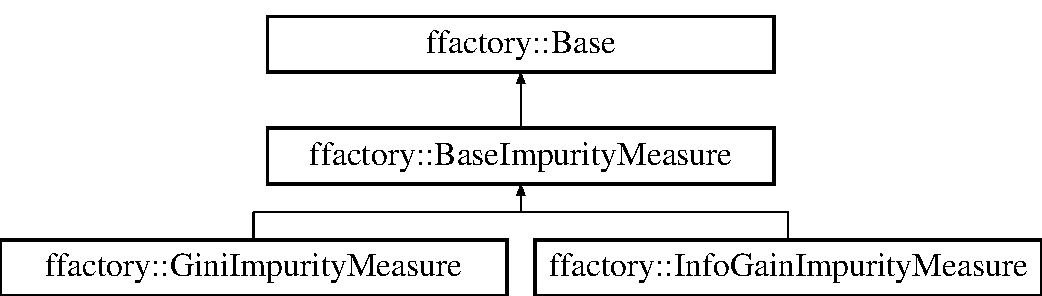
\includegraphics[height=3.000000cm]{classffactory_1_1_base_impurity_measure}
\end{center}
\end{figure}
\subsection*{Public Member Functions}
\begin{DoxyCompactItemize}
\item 
virtual double \hyperlink{classffactory_1_1_base_impurity_measure_ad0e0127a42c1ece9658ebf07e2b26efe}{calculate} (double p)=0
\end{DoxyCompactItemize}


\subsection{Member Function Documentation}
\hypertarget{classffactory_1_1_base_impurity_measure_ad0e0127a42c1ece9658ebf07e2b26efe}{\index{ffactory\-::\-Base\-Impurity\-Measure@{ffactory\-::\-Base\-Impurity\-Measure}!calculate@{calculate}}
\index{calculate@{calculate}!ffactory::BaseImpurityMeasure@{ffactory\-::\-Base\-Impurity\-Measure}}
\subsubsection[{calculate}]{\setlength{\rightskip}{0pt plus 5cm}virtual double ffactory\-::\-Base\-Impurity\-Measure\-::calculate (
\begin{DoxyParamCaption}
\item[{double}]{p}
\end{DoxyParamCaption}
)\hspace{0.3cm}{\ttfamily [pure virtual]}}}\label{classffactory_1_1_base_impurity_measure_ad0e0127a42c1ece9658ebf07e2b26efe}
Impurity measure calculation method 

Implemented in \hyperlink{classffactory_1_1_gini_impurity_measure_afad0349dd370af15c9b3334cd33e9a70}{ffactory\-::\-Gini\-Impurity\-Measure}, and \hyperlink{classffactory_1_1_info_gain_impurity_measure_a1996955c9df6847f0fccdd36112655b3}{ffactory\-::\-Info\-Gain\-Impurity\-Measure}.



The documentation for this class was generated from the following file\-:\begin{DoxyCompactItemize}
\item 
src/classifiers/trees/impurity\-Measures/base\-Impurity\-Measure.\-h\end{DoxyCompactItemize}

\hypertarget{classffactory_1_1_base_node_quality_measurer}{\section{ffactory\-:\-:Base\-Node\-Quality\-Measurer Class Reference}
\label{classffactory_1_1_base_node_quality_measurer}\index{ffactory\-::\-Base\-Node\-Quality\-Measurer@{ffactory\-::\-Base\-Node\-Quality\-Measurer}}
}


{\ttfamily \#include $<$base\-Node\-Quality\-Measurer.\-h$>$}

Inheritance diagram for ffactory\-:\-:Base\-Node\-Quality\-Measurer\-:\begin{figure}[H]
\begin{center}
\leavevmode
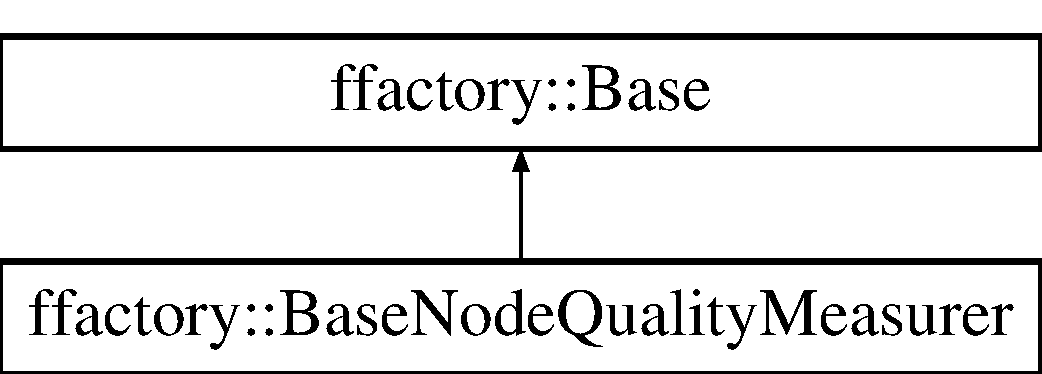
\includegraphics[height=2.000000cm]{classffactory_1_1_base_node_quality_measurer}
\end{center}
\end{figure}
\subsection*{Public Member Functions}
\begin{DoxyCompactItemize}
\item 
virtual Data\-Type \hyperlink{classffactory_1_1_base_node_quality_measurer_a2451bb93502b2350ba20e17f928ab313}{get\-Score} (\hyperlink{classffactory_1_1_binary_split}{Binary\-Split} $\ast$\hyperlink{namespaceffactory_a1fec00d28dbea621e480fd9f221d972e}{split}, \hyperlink{classffactory_1_1_dataset}{Dataset} $\ast$d, Mask\-Vector $\ast$mask)=0
\item 
\hypertarget{classffactory_1_1_base_node_quality_measurer_a4da2a8c3bf717d62cb1263922585522a}{virtual void {\bfseries Fill\-Best\-Node} (\hyperlink{classffactory_1_1_base_tree_node}{Base\-Tree\-Node} N)}\label{classffactory_1_1_base_node_quality_measurer_a4da2a8c3bf717d62cb1263922585522a}

\item 
\hypertarget{classffactory_1_1_base_node_quality_measurer_a34d90b57839b4f4187d16b88db6f9b87}{\hyperlink{classffactory_1_1_base_impurity_measure}{Base\-Impurity\-Measure} $\ast$ {\bfseries get\-Impurity\-Measure\-Function} ()}\label{classffactory_1_1_base_node_quality_measurer_a34d90b57839b4f4187d16b88db6f9b87}

\item 
\hypertarget{classffactory_1_1_base_node_quality_measurer_a34306d184defa83f0608a3cd5a5c6e32}{void {\bfseries set\-Impurity\-Measure\-Function} (Base\-Impurity\-Measure\-Unique\-Ptr impurity\-Function)}\label{classffactory_1_1_base_node_quality_measurer_a34306d184defa83f0608a3cd5a5c6e32}

\item 
virtual std\-::string \hyperlink{classffactory_1_1_base_node_quality_measurer_a7d93ff368d8b2b439c0f7310213bf63f}{get\-Info} ()
\end{DoxyCompactItemize}


\subsection{Detailed Description}
Tool to inspect node split quality 

\subsection{Member Function Documentation}
\hypertarget{classffactory_1_1_base_node_quality_measurer_a7d93ff368d8b2b439c0f7310213bf63f}{\index{ffactory\-::\-Base\-Node\-Quality\-Measurer@{ffactory\-::\-Base\-Node\-Quality\-Measurer}!get\-Info@{get\-Info}}
\index{get\-Info@{get\-Info}!ffactory::BaseNodeQualityMeasurer@{ffactory\-::\-Base\-Node\-Quality\-Measurer}}
\subsubsection[{get\-Info}]{\setlength{\rightskip}{0pt plus 5cm}virtual std\-::string ffactory\-::\-Base\-Node\-Quality\-Measurer\-::get\-Info (
\begin{DoxyParamCaption}
{}
\end{DoxyParamCaption}
)\hspace{0.3cm}{\ttfamily [inline]}, {\ttfamily [virtual]}}}\label{classffactory_1_1_base_node_quality_measurer_a7d93ff368d8b2b439c0f7310213bf63f}
Generates information string \begin{DoxyReturn}{Returns}
std\-::string contains information about object 
\end{DoxyReturn}


Reimplemented from \hyperlink{classffactory_1_1_base_a061e6165abeadad3fac626253d14a0c6}{ffactory\-::\-Base}.

\hypertarget{classffactory_1_1_base_node_quality_measurer_a2451bb93502b2350ba20e17f928ab313}{\index{ffactory\-::\-Base\-Node\-Quality\-Measurer@{ffactory\-::\-Base\-Node\-Quality\-Measurer}!get\-Score@{get\-Score}}
\index{get\-Score@{get\-Score}!ffactory::BaseNodeQualityMeasurer@{ffactory\-::\-Base\-Node\-Quality\-Measurer}}
\subsubsection[{get\-Score}]{\setlength{\rightskip}{0pt plus 5cm}virtual Data\-Type ffactory\-::\-Base\-Node\-Quality\-Measurer\-::get\-Score (
\begin{DoxyParamCaption}
\item[{{\bf Binary\-Split} $\ast$}]{split, }
\item[{{\bf Dataset} $\ast$}]{d, }
\item[{Mask\-Vector $\ast$}]{mask}
\end{DoxyParamCaption}
)\hspace{0.3cm}{\ttfamily [pure virtual]}}}\label{classffactory_1_1_base_node_quality_measurer_a2451bb93502b2350ba20e17f928ab313}
Obtain {\itshape split} quality on dataset {\itshape d} maksed with {\itshape mask} 
\begin{DoxyParams}{Parameters}
{\em split} & \\
\hline
{\em d} & \\
\hline
{\em mask} & \\
\hline
\end{DoxyParams}
\begin{DoxyReturn}{Returns}
Data\-Type value 
\end{DoxyReturn}


The documentation for this class was generated from the following file\-:\begin{DoxyCompactItemize}
\item 
src/classifiers/trees/splits/quality\-Measurer/base\-Node\-Quality\-Measurer.\-h\end{DoxyCompactItemize}

\hypertarget{classffactory_1_1_base_online_classifier}{\section{ffactory\-:\-:Base\-Online\-Classifier Class Reference}
\label{classffactory_1_1_base_online_classifier}\index{ffactory\-::\-Base\-Online\-Classifier@{ffactory\-::\-Base\-Online\-Classifier}}
}


{\ttfamily \#include $<$Base\-Online\-Classifier.\-h$>$}

Inheritance diagram for ffactory\-:\-:Base\-Online\-Classifier\-:\begin{figure}[H]
\begin{center}
\leavevmode
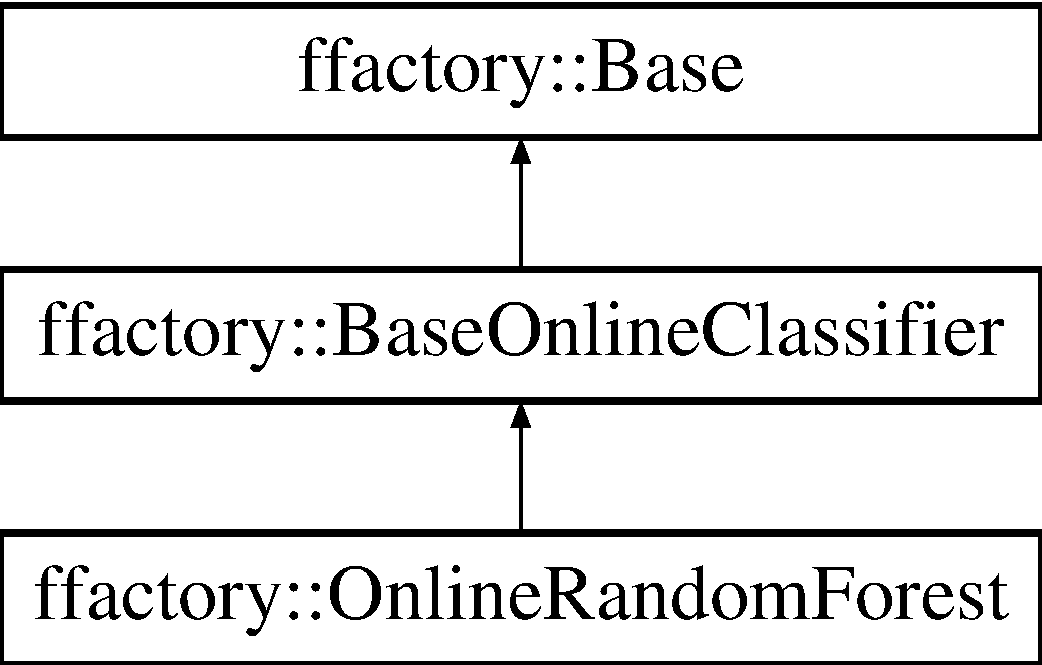
\includegraphics[height=3.000000cm]{classffactory_1_1_base_online_classifier}
\end{center}
\end{figure}
\subsection*{Public Member Functions}
\begin{DoxyCompactItemize}
\item 
virtual double \hyperlink{classffactory_1_1_base_online_classifier_a1f4c58973708b188e99651ed0b82631d}{update} (\hyperlink{classffactory_1_1_dataset}{Dataset} $\ast$newdata)
\item 
virtual double \hyperlink{classffactory_1_1_base_online_classifier_ae2ea31e0e89fb2131dda743d9803856b}{update} (\hyperlink{classffactory_1_1_sample}{Sample} $\ast$newdata)=0
\end{DoxyCompactItemize}


\subsection{Detailed Description}
\hyperlink{classffactory_1_1_base}{Base} class for all Online Classifiers 

\subsection{Member Function Documentation}
\hypertarget{classffactory_1_1_base_online_classifier_a1f4c58973708b188e99651ed0b82631d}{\index{ffactory\-::\-Base\-Online\-Classifier@{ffactory\-::\-Base\-Online\-Classifier}!update@{update}}
\index{update@{update}!ffactory::BaseOnlineClassifier@{ffactory\-::\-Base\-Online\-Classifier}}
\subsubsection[{update}]{\setlength{\rightskip}{0pt plus 5cm}virtual double ffactory\-::\-Base\-Online\-Classifier\-::update (
\begin{DoxyParamCaption}
\item[{{\bf Dataset} $\ast$}]{newdata}
\end{DoxyParamCaption}
)\hspace{0.3cm}{\ttfamily [inline]}, {\ttfamily [virtual]}}}\label{classffactory_1_1_base_online_classifier_a1f4c58973708b188e99651ed0b82631d}
Main class for update model with {\itshape newdata} 

Reimplemented in \hyperlink{classffactory_1_1_online_random_forest_af0c36073053407883c7ddd1fce631d7f}{ffactory\-::\-Online\-Random\-Forest}.

\hypertarget{classffactory_1_1_base_online_classifier_ae2ea31e0e89fb2131dda743d9803856b}{\index{ffactory\-::\-Base\-Online\-Classifier@{ffactory\-::\-Base\-Online\-Classifier}!update@{update}}
\index{update@{update}!ffactory::BaseOnlineClassifier@{ffactory\-::\-Base\-Online\-Classifier}}
\subsubsection[{update}]{\setlength{\rightskip}{0pt plus 5cm}virtual double ffactory\-::\-Base\-Online\-Classifier\-::update (
\begin{DoxyParamCaption}
\item[{{\bf Sample} $\ast$}]{newdata}
\end{DoxyParamCaption}
)\hspace{0.3cm}{\ttfamily [pure virtual]}}}\label{classffactory_1_1_base_online_classifier_ae2ea31e0e89fb2131dda743d9803856b}
Main class for update model with {\itshape newdata} 

The documentation for this class was generated from the following file\-:\begin{DoxyCompactItemize}
\item 
src/classifiers/Base\-Online\-Classifier.\-h\end{DoxyCompactItemize}

\hypertarget{classffactory_1_1_base_online_node}{\section{ffactory\-:\-:Base\-Online\-Node Class Reference}
\label{classffactory_1_1_base_online_node}\index{ffactory\-::\-Base\-Online\-Node@{ffactory\-::\-Base\-Online\-Node}}
}
Inheritance diagram for ffactory\-:\-:Base\-Online\-Node\-:\begin{figure}[H]
\begin{center}
\leavevmode
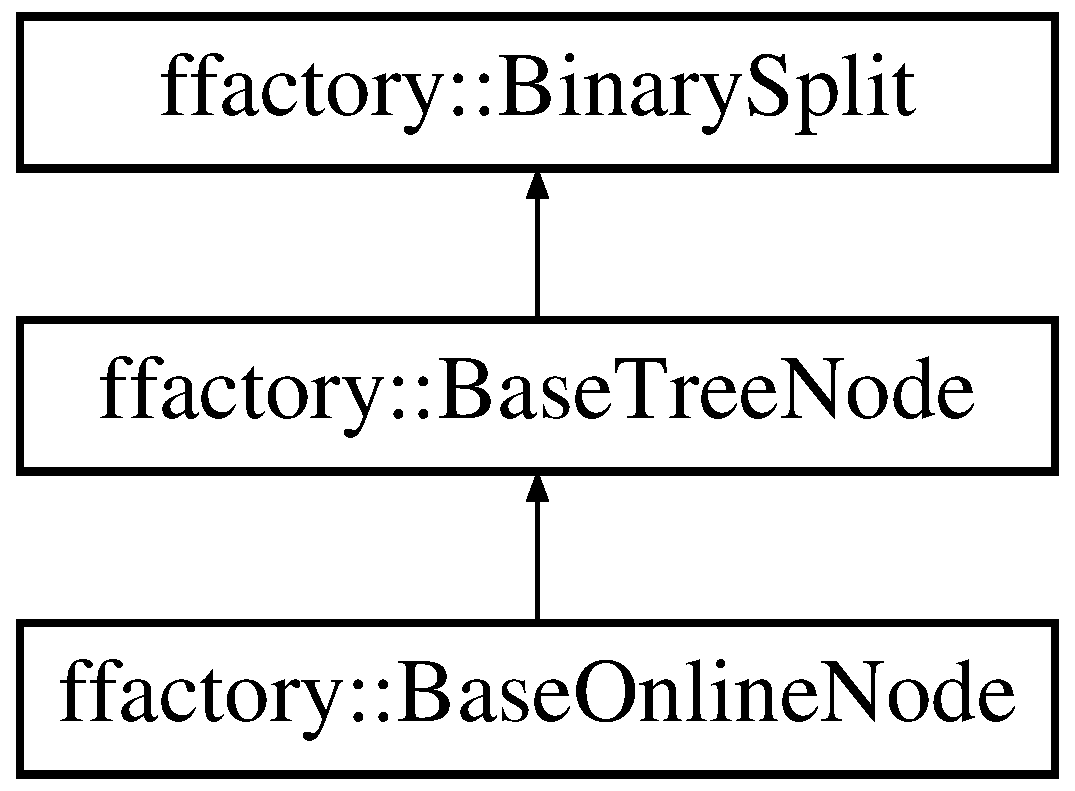
\includegraphics[height=3.000000cm]{classffactory_1_1_base_online_node}
\end{center}
\end{figure}
\subsection*{Public Member Functions}
\begin{DoxyCompactItemize}
\item 
virtual double \hyperlink{classffactory_1_1_base_online_node_aae14e67d789d867081aa9dbdb55181cf}{update} (\hyperlink{classffactory_1_1_sample}{Sample} $\ast$newdata)
\item 
\hypertarget{classffactory_1_1_base_online_node_aafd8784835b48a03fb7729cd926855e6}{\hyperlink{classffactory_1_1_base_online_node}{Base\-Online\-Node} \& {\bfseries operator=} (\hyperlink{classffactory_1_1_base_tree_node}{Base\-Tree\-Node} arg)}\label{classffactory_1_1_base_online_node_aafd8784835b48a03fb7729cd926855e6}

\end{DoxyCompactItemize}


\subsection{Member Function Documentation}
\hypertarget{classffactory_1_1_base_online_node_aae14e67d789d867081aa9dbdb55181cf}{\index{ffactory\-::\-Base\-Online\-Node@{ffactory\-::\-Base\-Online\-Node}!update@{update}}
\index{update@{update}!ffactory::BaseOnlineNode@{ffactory\-::\-Base\-Online\-Node}}
\subsubsection[{update}]{\setlength{\rightskip}{0pt plus 5cm}virtual double ffactory\-::\-Base\-Online\-Node\-::update (
\begin{DoxyParamCaption}
\item[{{\bf Sample} $\ast$}]{newdata}
\end{DoxyParamCaption}
)\hspace{0.3cm}{\ttfamily [inline]}, {\ttfamily [virtual]}}}\label{classffactory_1_1_base_online_node_aae14e67d789d867081aa9dbdb55181cf}
Main class for update model with {\itshape newdata} 

The documentation for this class was generated from the following file\-:\begin{DoxyCompactItemize}
\item 
src/classifiers/trees/Base\-Online\-Node.\-h\end{DoxyCompactItemize}

\hypertarget{classffactory_1_1_base_online_property}{\section{ffactory\-:\-:Base\-Online\-Property Class Reference}
\label{classffactory_1_1_base_online_property}\index{ffactory\-::\-Base\-Online\-Property@{ffactory\-::\-Base\-Online\-Property}}
}


{\ttfamily \#include $<$Base\-Online\-Property.\-h$>$}

Inheritance diagram for ffactory\-:\-:Base\-Online\-Property\-:\begin{figure}[H]
\begin{center}
\leavevmode
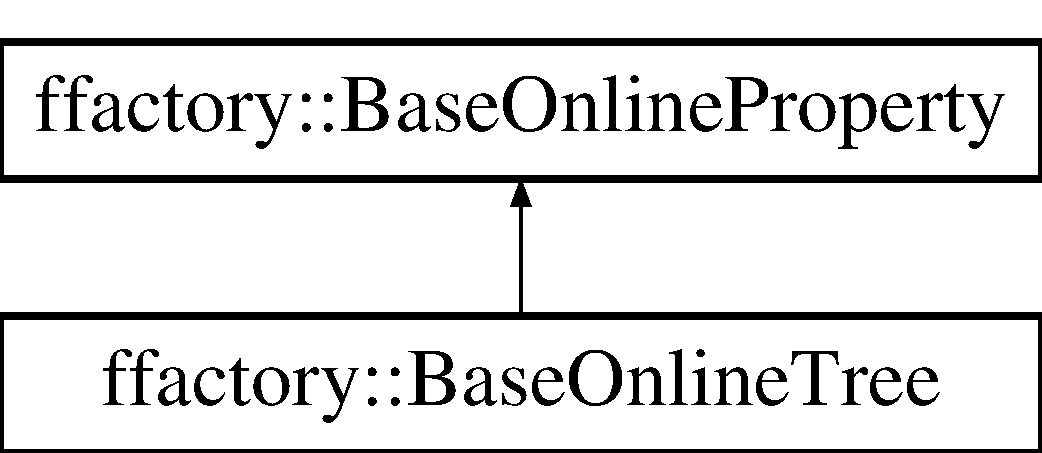
\includegraphics[height=2.000000cm]{classffactory_1_1_base_online_property}
\end{center}
\end{figure}
\subsection*{Public Member Functions}
\begin{DoxyCompactItemize}
\item 
virtual double \hyperlink{classffactory_1_1_base_online_property_a9cfb11c90f0c4e0a21a6c2d2b871d2fa}{update} (\hyperlink{classffactory_1_1_dataset}{Dataset} $\ast$newdata)
\item 
virtual double \hyperlink{classffactory_1_1_base_online_property_a770c65109a57a4cca772cb3ec143fe68}{update} (\hyperlink{classffactory_1_1_sample}{Sample} $\ast$newdata)=0
\end{DoxyCompactItemize}


\subsection{Detailed Description}
\hyperlink{classffactory_1_1_base}{Base} class for all Online Classifiers 

\subsection{Member Function Documentation}
\hypertarget{classffactory_1_1_base_online_property_a9cfb11c90f0c4e0a21a6c2d2b871d2fa}{\index{ffactory\-::\-Base\-Online\-Property@{ffactory\-::\-Base\-Online\-Property}!update@{update}}
\index{update@{update}!ffactory::BaseOnlineProperty@{ffactory\-::\-Base\-Online\-Property}}
\subsubsection[{update}]{\setlength{\rightskip}{0pt plus 5cm}virtual double ffactory\-::\-Base\-Online\-Property\-::update (
\begin{DoxyParamCaption}
\item[{{\bf Dataset} $\ast$}]{newdata}
\end{DoxyParamCaption}
)\hspace{0.3cm}{\ttfamily [inline]}, {\ttfamily [virtual]}}}\label{classffactory_1_1_base_online_property_a9cfb11c90f0c4e0a21a6c2d2b871d2fa}
Main class for update model with {\itshape newdata} \hypertarget{classffactory_1_1_base_online_property_a770c65109a57a4cca772cb3ec143fe68}{\index{ffactory\-::\-Base\-Online\-Property@{ffactory\-::\-Base\-Online\-Property}!update@{update}}
\index{update@{update}!ffactory::BaseOnlineProperty@{ffactory\-::\-Base\-Online\-Property}}
\subsubsection[{update}]{\setlength{\rightskip}{0pt plus 5cm}virtual double ffactory\-::\-Base\-Online\-Property\-::update (
\begin{DoxyParamCaption}
\item[{{\bf Sample} $\ast$}]{newdata}
\end{DoxyParamCaption}
)\hspace{0.3cm}{\ttfamily [pure virtual]}}}\label{classffactory_1_1_base_online_property_a770c65109a57a4cca772cb3ec143fe68}
Main class for update model with {\itshape newdata} 

Implemented in \hyperlink{classffactory_1_1_base_online_tree_a89983c60bab64b9f4c0946bf8c1ba40d}{ffactory\-::\-Base\-Online\-Tree}.



The documentation for this class was generated from the following file\-:\begin{DoxyCompactItemize}
\item 
src/classifiers/properties/Base\-Online\-Property.\-h\end{DoxyCompactItemize}

\hypertarget{classffactory_1_1_base_online_tree}{\section{ffactory\-:\-:Base\-Online\-Tree Class Reference}
\label{classffactory_1_1_base_online_tree}\index{ffactory\-::\-Base\-Online\-Tree@{ffactory\-::\-Base\-Online\-Tree}}
}
Inheritance diagram for ffactory\-:\-:Base\-Online\-Tree\-:\begin{figure}[H]
\begin{center}
\leavevmode
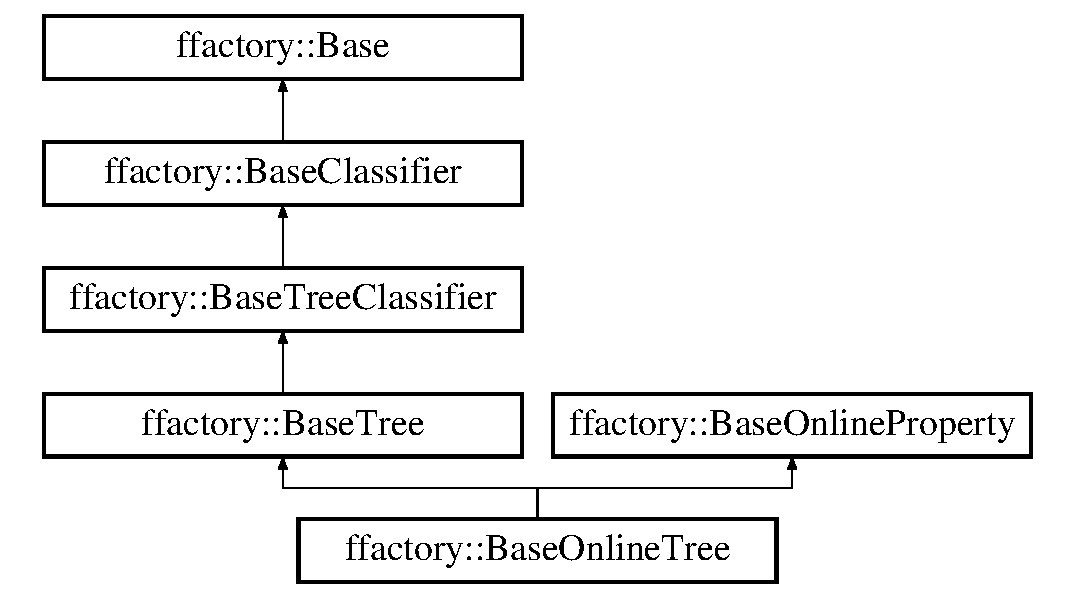
\includegraphics[height=5.000000cm]{classffactory_1_1_base_online_tree}
\end{center}
\end{figure}
\subsection*{Public Member Functions}
\begin{DoxyCompactItemize}
\item 
virtual std\-::string \hyperlink{classffactory_1_1_base_online_tree_ad814d53893b7321f3384677b864ba2de}{get\-Info} ()
\item 
virtual double \hyperlink{classffactory_1_1_base_online_tree_a89983c60bab64b9f4c0946bf8c1ba40d}{update} (\hyperlink{classffactory_1_1_sample}{Sample} $\ast$newdata)
\end{DoxyCompactItemize}
\subsection*{Additional Inherited Members}


\subsection{Member Function Documentation}
\hypertarget{classffactory_1_1_base_online_tree_ad814d53893b7321f3384677b864ba2de}{\index{ffactory\-::\-Base\-Online\-Tree@{ffactory\-::\-Base\-Online\-Tree}!get\-Info@{get\-Info}}
\index{get\-Info@{get\-Info}!ffactory::BaseOnlineTree@{ffactory\-::\-Base\-Online\-Tree}}
\subsubsection[{get\-Info}]{\setlength{\rightskip}{0pt plus 5cm}virtual std\-::string ffactory\-::\-Base\-Online\-Tree\-::get\-Info (
\begin{DoxyParamCaption}
{}
\end{DoxyParamCaption}
)\hspace{0.3cm}{\ttfamily [inline]}, {\ttfamily [virtual]}}}\label{classffactory_1_1_base_online_tree_ad814d53893b7321f3384677b864ba2de}
Generates information string \begin{DoxyReturn}{Returns}
std\-::string contains information about classifier 
\end{DoxyReturn}
\begin{DoxyRefDesc}{Todo}
\item[\hyperlink{todo__todo000003}{Todo}]Написать вывод полной инфы о дереве \end{DoxyRefDesc}


Reimplemented from \hyperlink{classffactory_1_1_base_tree_a21d7faa1c68bb531522a73c36b10a95c}{ffactory\-::\-Base\-Tree}.

\hypertarget{classffactory_1_1_base_online_tree_a89983c60bab64b9f4c0946bf8c1ba40d}{\index{ffactory\-::\-Base\-Online\-Tree@{ffactory\-::\-Base\-Online\-Tree}!update@{update}}
\index{update@{update}!ffactory::BaseOnlineTree@{ffactory\-::\-Base\-Online\-Tree}}
\subsubsection[{update}]{\setlength{\rightskip}{0pt plus 5cm}virtual double ffactory\-::\-Base\-Online\-Tree\-::update (
\begin{DoxyParamCaption}
\item[{{\bf Sample} $\ast$}]{newdata}
\end{DoxyParamCaption}
)\hspace{0.3cm}{\ttfamily [inline]}, {\ttfamily [virtual]}}}\label{classffactory_1_1_base_online_tree_a89983c60bab64b9f4c0946bf8c1ba40d}
Main class for update model with {\itshape newdata} 

Implements \hyperlink{classffactory_1_1_base_online_property_a770c65109a57a4cca772cb3ec143fe68}{ffactory\-::\-Base\-Online\-Property}.



The documentation for this class was generated from the following files\-:\begin{DoxyCompactItemize}
\item 
src/classifiers/trees/Base\-Online\-Tree.\-h\item 
src/classifiers/trees/Base\-Online\-Tree.\-cpp\end{DoxyCompactItemize}

\hypertarget{classffactory_1_1_base_preprocessor}{\section{ffactory\-:\-:Base\-Preprocessor Class Reference}
\label{classffactory_1_1_base_preprocessor}\index{ffactory\-::\-Base\-Preprocessor@{ffactory\-::\-Base\-Preprocessor}}
}


{\ttfamily \#include $<$Base\-Preprocessor.\-h$>$}

Inheritance diagram for ffactory\-:\-:Base\-Preprocessor\-:\begin{figure}[H]
\begin{center}
\leavevmode
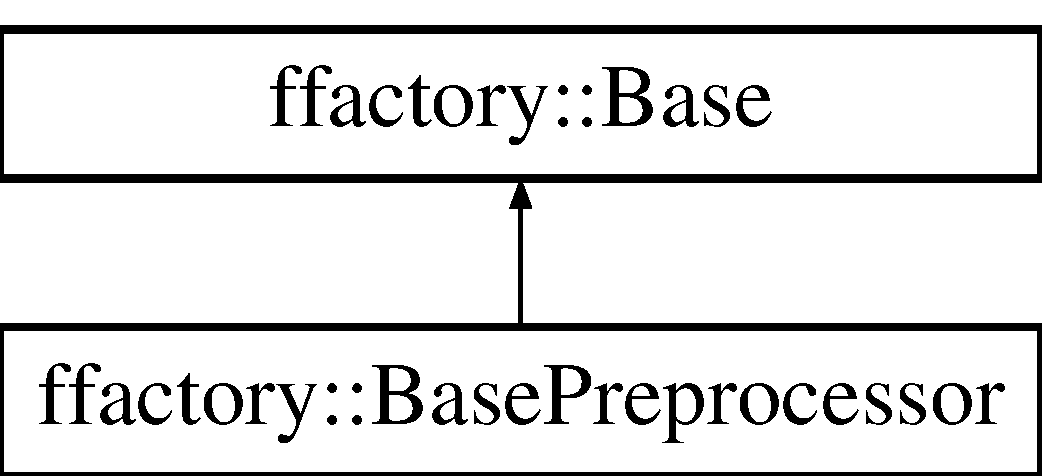
\includegraphics[height=2.000000cm]{classffactory_1_1_base_preprocessor}
\end{center}
\end{figure}
\subsection*{Public Member Functions}
\begin{DoxyCompactItemize}
\item 
\hypertarget{classffactory_1_1_base_preprocessor_aba9d0e28cb40fa8e7fce41cf97ddaf98}{{\bfseries base\-Preprocessor} ()}\label{classffactory_1_1_base_preprocessor_aba9d0e28cb40fa8e7fce41cf97ddaf98}

\item 
virtual \hyperlink{classffactory_1_1_dataset}{Dataset} $\ast$ \hyperlink{classffactory_1_1_base_preprocessor_add6380a587d34d4bf295f85056abaddd}{preprocess} (\hyperlink{classffactory_1_1_dataset}{Dataset} d)
\end{DoxyCompactItemize}


\subsection{Detailed Description}
Virtual class for data preprocessing 

\subsection{Member Function Documentation}
\hypertarget{classffactory_1_1_base_preprocessor_add6380a587d34d4bf295f85056abaddd}{\index{ffactory\-::\-Base\-Preprocessor@{ffactory\-::\-Base\-Preprocessor}!preprocess@{preprocess}}
\index{preprocess@{preprocess}!ffactory::BasePreprocessor@{ffactory\-::\-Base\-Preprocessor}}
\subsubsection[{preprocess}]{\setlength{\rightskip}{0pt plus 5cm}virtual {\bf Dataset}$\ast$ ffactory\-::\-Base\-Preprocessor\-::preprocess (
\begin{DoxyParamCaption}
\item[{{\bf Dataset}}]{d}
\end{DoxyParamCaption}
)\hspace{0.3cm}{\ttfamily [virtual]}}}\label{classffactory_1_1_base_preprocessor_add6380a587d34d4bf295f85056abaddd}
Data preprocessing routine 
\begin{DoxyParams}{Parameters}
{\em d} & input dataset \\
\hline
\end{DoxyParams}
\begin{DoxyReturn}{Returns}
output dataset pointer 
\end{DoxyReturn}


The documentation for this class was generated from the following file\-:\begin{DoxyCompactItemize}
\item 
src/preprocessors/Base\-Preprocessor.\-h\end{DoxyCompactItemize}

\hypertarget{classffactory_1_1_base_split}{\section{ffactory\-:\-:Base\-Split Class Reference}
\label{classffactory_1_1_base_split}\index{ffactory\-::\-Base\-Split@{ffactory\-::\-Base\-Split}}
}


{\ttfamily \#include $<$base\-Split.\-h$>$}

\subsection*{Public Member Functions}
\begin{DoxyCompactItemize}
\item 
\hypertarget{classffactory_1_1_base_split_a0d58b369b12890e76ea0548c9fdab217}{Index\-Vector {\bfseries get\-Feature\-Index} () const }\label{classffactory_1_1_base_split_a0d58b369b12890e76ea0548c9fdab217}

\item 
\hypertarget{classffactory_1_1_base_split_a078ac711bddfb871e5473a1fa3da124f}{void {\bfseries set\-Feature\-Index\-Set} (Index\-Vector \&feature\-Index\-Set)}\label{classffactory_1_1_base_split_a078ac711bddfb871e5473a1fa3da124f}

\item 
\hypertarget{classffactory_1_1_base_split_abbccdac7fa366b151326b730aa6ccf38}{Data\-Vector {\bfseries get\-Feature\-Value} () const }\label{classffactory_1_1_base_split_abbccdac7fa366b151326b730aa6ccf38}

\item 
\hypertarget{classffactory_1_1_base_split_adaa4d2651f77b5946b487cac0d45c4cb}{void {\bfseries set\-Feature\-Value} (double feature\-Value)}\label{classffactory_1_1_base_split_adaa4d2651f77b5946b487cac0d45c4cb}

\item 
virtual bool \hyperlink{classffactory_1_1_base_split_a86e2a328692f90e3993b117ce17bf452}{decide} (Data\-Vector feature\-Vector)
\item 
virtual Data\-Type \hyperlink{classffactory_1_1_base_split_ae2195df1e6a0f7774e12c65a89975f4c}{get\-Impurity\-Score} (\hyperlink{classffactory_1_1_dataset}{Dataset} d)=0
\item 
\hypertarget{classffactory_1_1_base_split_a7151988e8ff47ef87890da1b08f9008b}{\hyperlink{classffactory_1_1_base_impurity_measure}{Base\-Impurity\-Measure} $\ast$ {\bfseries get\-Impurity\-Measure\-Function} ()}\label{classffactory_1_1_base_split_a7151988e8ff47ef87890da1b08f9008b}

\item 
\hypertarget{classffactory_1_1_base_split_a3edcedf23d144f69e04693f7a5fd8de8}{void {\bfseries set\-Impurity\-Measure\-Function} (\hyperlink{classffactory_1_1_base_impurity_measure}{Base\-Impurity\-Measure} $\ast$impurity\-Function)}\label{classffactory_1_1_base_split_a3edcedf23d144f69e04693f7a5fd8de8}

\end{DoxyCompactItemize}


\subsection{Detailed Description}
Split abstraction to get interface to many types of linear splits (axial-\/parallel and oblique) 

\subsection{Member Function Documentation}
\hypertarget{classffactory_1_1_base_split_a86e2a328692f90e3993b117ce17bf452}{\index{ffactory\-::\-Base\-Split@{ffactory\-::\-Base\-Split}!decide@{decide}}
\index{decide@{decide}!ffactory::BaseSplit@{ffactory\-::\-Base\-Split}}
\subsubsection[{decide}]{\setlength{\rightskip}{0pt plus 5cm}virtual bool ffactory\-::\-Base\-Split\-::decide (
\begin{DoxyParamCaption}
\item[{Data\-Vector}]{feature\-Vector}
\end{DoxyParamCaption}
)\hspace{0.3cm}{\ttfamily [virtual]}}}\label{classffactory_1_1_base_split_a86e2a328692f90e3993b117ce17bf452}
Used to perform split decision 
\begin{DoxyParams}{Parameters}
{\em feature\-Vector} & \\
\hline
\end{DoxyParams}
\begin{DoxyReturn}{Returns}

\end{DoxyReturn}
\hypertarget{classffactory_1_1_base_split_ae2195df1e6a0f7774e12c65a89975f4c}{\index{ffactory\-::\-Base\-Split@{ffactory\-::\-Base\-Split}!get\-Impurity\-Score@{get\-Impurity\-Score}}
\index{get\-Impurity\-Score@{get\-Impurity\-Score}!ffactory::BaseSplit@{ffactory\-::\-Base\-Split}}
\subsubsection[{get\-Impurity\-Score}]{\setlength{\rightskip}{0pt plus 5cm}virtual Data\-Type ffactory\-::\-Base\-Split\-::get\-Impurity\-Score (
\begin{DoxyParamCaption}
\item[{{\bf Dataset}}]{d}
\end{DoxyParamCaption}
)\hspace{0.3cm}{\ttfamily [pure virtual]}}}\label{classffactory_1_1_base_split_ae2195df1e6a0f7774e12c65a89975f4c}
Calculate impurity to obtain split quality on dataset {\itshape d} 
\begin{DoxyParams}{Parameters}
{\em d} & \hyperlink{classffactory_1_1_dataset}{Dataset} \\
\hline
\end{DoxyParams}
\begin{DoxyReturn}{Returns}
Quality score of split 
\end{DoxyReturn}


The documentation for this class was generated from the following file\-:\begin{DoxyCompactItemize}
\item 
src/classifiers/trees/splits/base\-Split.\-h\end{DoxyCompactItemize}

\hypertarget{classffactory_1_1_base_split_candidate_generator}{\section{ffactory\-:\-:Base\-Split\-Candidate\-Generator Class Reference}
\label{classffactory_1_1_base_split_candidate_generator}\index{ffactory\-::\-Base\-Split\-Candidate\-Generator@{ffactory\-::\-Base\-Split\-Candidate\-Generator}}
}


{\ttfamily \#include $<$Base\-Split\-Candidate\-Generator.\-h$>$}

Inheritance diagram for ffactory\-:\-:Base\-Split\-Candidate\-Generator\-:\begin{figure}[H]
\begin{center}
\leavevmode
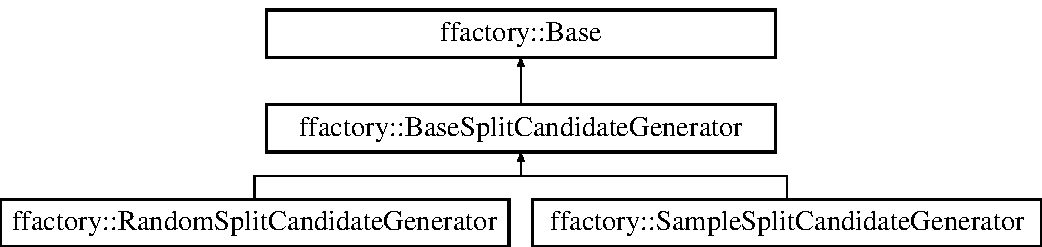
\includegraphics[height=3.000000cm]{classffactory_1_1_base_split_candidate_generator}
\end{center}
\end{figure}
\subsection*{Public Member Functions}
\begin{DoxyCompactItemize}
\item 
virtual void \hyperlink{classffactory_1_1_base_split_candidate_generator_a79da89383882bdad7a846f5458f794b2}{generate} (\hyperlink{classffactory_1_1_data_ranges}{Data\-Ranges} $\ast$ranges=N\-U\-L\-L)=0
\item 
\hypertarget{classffactory_1_1_base_split_candidate_generator_a06ae19f61d89d902ef414140c329e352}{\hyperlink{classffactory_1_1_dataset}{Dataset} $\ast$ {\bfseries get\-Dataset} () const }\label{classffactory_1_1_base_split_candidate_generator_a06ae19f61d89d902ef414140c329e352}

\item 
\hypertarget{classffactory_1_1_base_split_candidate_generator_a0a136267dcff55a7647c143e0013a0eb}{void {\bfseries set\-Dataset} (\hyperlink{classffactory_1_1_dataset}{Dataset} $\ast$dataset)}\label{classffactory_1_1_base_split_candidate_generator_a0a136267dcff55a7647c143e0013a0eb}

\item 
\hypertarget{classffactory_1_1_base_split_candidate_generator_ac1582c41b1106b418edc66fa3b580396}{const Index\-Vector \& {\bfseries get\-Feature\-Mask} () const }\label{classffactory_1_1_base_split_candidate_generator_ac1582c41b1106b418edc66fa3b580396}

\item 
\hypertarget{classffactory_1_1_base_split_candidate_generator_ad748feb93b561c2480a837cba7a3d120}{void {\bfseries set\-Feature\-Mask} (Index\-Vector \&\hyperlink{classffactory_1_1_base_split_candidate_generator_a7ce11df8208d85d2da2914e41ab3467c}{feature\-Mask})}\label{classffactory_1_1_base_split_candidate_generator_ad748feb93b561c2480a837cba7a3d120}

\item 
\hypertarget{classffactory_1_1_base_split_candidate_generator_a3a468c1b216203b46921fd50bab5e8b0}{bool {\bfseries is\-Use\-All\-Features} () const }\label{classffactory_1_1_base_split_candidate_generator_a3a468c1b216203b46921fd50bab5e8b0}

\item 
\hypertarget{classffactory_1_1_base_split_candidate_generator_a0a6e2fa82711f2c6b4e5494b57a59cbd}{void {\bfseries set\-Use\-All\-Features} (bool \hyperlink{classffactory_1_1_base_split_candidate_generator_afe4971fb46570d6658dad28eefe6d52c}{use\-All\-Features})}\label{classffactory_1_1_base_split_candidate_generator_a0a6e2fa82711f2c6b4e5494b57a59cbd}

\item 
\hypertarget{classffactory_1_1_base_split_candidate_generator_a0659fe8d120a3a7aa9c30cb3c3574325}{std\-::vector$<$ \hyperlink{classffactory_1_1_binary_split}{Binary\-Split} $>$ $\ast$ {\bfseries get\-Split\-Set} ()}\label{classffactory_1_1_base_split_candidate_generator_a0659fe8d120a3a7aa9c30cb3c3574325}

\item 
\hypertarget{classffactory_1_1_base_split_candidate_generator_ab73c817c35e6b157b1ca895310fb32fc}{\hyperlink{classffactory_1_1_binary_split}{Binary\-Split} $\ast$ {\bfseries get\-Split} (Index\-Type s)}\label{classffactory_1_1_base_split_candidate_generator_ab73c817c35e6b157b1ca895310fb32fc}

\item 
\hypertarget{classffactory_1_1_base_split_candidate_generator_a4b797e166584d14635d18554b0ca362d}{Index\-Type {\bfseries get\-Split\-Num} ()}\label{classffactory_1_1_base_split_candidate_generator_a4b797e166584d14635d18554b0ca362d}

\item 
\hypertarget{classffactory_1_1_base_split_candidate_generator_a78c52e1595eb6bc7efb2aad2eb563f8d}{void {\bfseries add\-Split} (\hyperlink{classffactory_1_1_binary_split}{Binary\-Split} \&\hyperlink{namespaceffactory_a1fec00d28dbea621e480fd9f221d972e}{split})}\label{classffactory_1_1_base_split_candidate_generator_a78c52e1595eb6bc7efb2aad2eb563f8d}

\item 
\hypertarget{classffactory_1_1_base_split_candidate_generator_af4688a53f51dfe8d590e1f769cd477ed}{void {\bfseries check\-Data} ()}\label{classffactory_1_1_base_split_candidate_generator_af4688a53f51dfe8d590e1f769cd477ed}

\item 
\hypertarget{classffactory_1_1_base_split_candidate_generator_ae6130b02482da9be8400b703e8aee9f4}{unsigned int {\bfseries get\-Num\-Features} ()}\label{classffactory_1_1_base_split_candidate_generator_ae6130b02482da9be8400b703e8aee9f4}

\item 
\hypertarget{classffactory_1_1_base_split_candidate_generator_aa6687b253e20b56badcd1b430c47c886}{void {\bfseries set\-Num\-Features} (unsigned int \-\_\-num\-Features)}\label{classffactory_1_1_base_split_candidate_generator_aa6687b253e20b56badcd1b430c47c886}

\item 
std\-::string \hyperlink{classffactory_1_1_base_split_candidate_generator_a9247b20b96b60d227f3f3484e5614f39}{get\-Info} ()
\item 
void \hyperlink{classffactory_1_1_base_split_candidate_generator_a0f10f06053c5d623e9d7b30afdfc319e}{clear} ()
\end{DoxyCompactItemize}
\subsection*{Protected Attributes}
\begin{DoxyCompactItemize}
\item 
\hypertarget{classffactory_1_1_base_split_candidate_generator_a4df63e753be1dca1c2ffca46d8609148}{\hyperlink{classffactory_1_1_dataset}{Dataset} $\ast$ {\bfseries dataset}}\label{classffactory_1_1_base_split_candidate_generator_a4df63e753be1dca1c2ffca46d8609148}

\item 
bool \hyperlink{classffactory_1_1_base_split_candidate_generator_afe4971fb46570d6658dad28eefe6d52c}{use\-All\-Features}
\item 
Index\-Vector \hyperlink{classffactory_1_1_base_split_candidate_generator_a7ce11df8208d85d2da2914e41ab3467c}{feature\-Mask}
\item 
Index\-Type \hyperlink{classffactory_1_1_base_split_candidate_generator_a418bcf78922a3d288de0ae3ec55553a6}{num\-Features}
\item 
\hypertarget{classffactory_1_1_base_split_candidate_generator_ad7d567911eda56ede547463b773b18d2}{Split\-Vector {\bfseries split\-Set}}\label{classffactory_1_1_base_split_candidate_generator_ad7d567911eda56ede547463b773b18d2}

\end{DoxyCompactItemize}


\subsection{Detailed Description}
\hyperlink{classffactory_1_1_base}{Base} class for split candidate generators. The class spawns splits which will be examined and the best split will be found. 

\subsection{Member Function Documentation}
\hypertarget{classffactory_1_1_base_split_candidate_generator_a0f10f06053c5d623e9d7b30afdfc319e}{\index{ffactory\-::\-Base\-Split\-Candidate\-Generator@{ffactory\-::\-Base\-Split\-Candidate\-Generator}!clear@{clear}}
\index{clear@{clear}!ffactory::BaseSplitCandidateGenerator@{ffactory\-::\-Base\-Split\-Candidate\-Generator}}
\subsubsection[{clear}]{\setlength{\rightskip}{0pt plus 5cm}void ffactory\-::\-Base\-Split\-Candidate\-Generator\-::clear (
\begin{DoxyParamCaption}
{}
\end{DoxyParamCaption}
)\hspace{0.3cm}{\ttfamily [inline]}}}\label{classffactory_1_1_base_split_candidate_generator_a0f10f06053c5d623e9d7b30afdfc319e}
Delete all the splits form buffer \hypertarget{classffactory_1_1_base_split_candidate_generator_a79da89383882bdad7a846f5458f794b2}{\index{ffactory\-::\-Base\-Split\-Candidate\-Generator@{ffactory\-::\-Base\-Split\-Candidate\-Generator}!generate@{generate}}
\index{generate@{generate}!ffactory::BaseSplitCandidateGenerator@{ffactory\-::\-Base\-Split\-Candidate\-Generator}}
\subsubsection[{generate}]{\setlength{\rightskip}{0pt plus 5cm}virtual void ffactory\-::\-Base\-Split\-Candidate\-Generator\-::generate (
\begin{DoxyParamCaption}
\item[{{\bf Data\-Ranges} $\ast$}]{ranges = {\ttfamily NULL}}
\end{DoxyParamCaption}
)\hspace{0.3cm}{\ttfamily [pure virtual]}}}\label{classffactory_1_1_base_split_candidate_generator_a79da89383882bdad7a846f5458f794b2}
Produce split-\/candidates using Mask\-Vector if {\itshape ranges} == 0 then dataset ranges will be used 
\begin{DoxyParams}{Parameters}
{\em ranges} & \\
\hline
\end{DoxyParams}


Implemented in \hyperlink{classffactory_1_1_random_split_candidate_generator_a488f87c1cc5ddccc44d5827db6f02964}{ffactory\-::\-Random\-Split\-Candidate\-Generator}, and \hyperlink{classffactory_1_1_sample_split_candidate_generator_a7a589641d4668c711e002a440c00a6b8}{ffactory\-::\-Sample\-Split\-Candidate\-Generator}.

\hypertarget{classffactory_1_1_base_split_candidate_generator_a9247b20b96b60d227f3f3484e5614f39}{\index{ffactory\-::\-Base\-Split\-Candidate\-Generator@{ffactory\-::\-Base\-Split\-Candidate\-Generator}!get\-Info@{get\-Info}}
\index{get\-Info@{get\-Info}!ffactory::BaseSplitCandidateGenerator@{ffactory\-::\-Base\-Split\-Candidate\-Generator}}
\subsubsection[{get\-Info}]{\setlength{\rightskip}{0pt plus 5cm}std\-::string ffactory\-::\-Base\-Split\-Candidate\-Generator\-::get\-Info (
\begin{DoxyParamCaption}
{}
\end{DoxyParamCaption}
)\hspace{0.3cm}{\ttfamily [inline]}, {\ttfamily [virtual]}}}\label{classffactory_1_1_base_split_candidate_generator_a9247b20b96b60d227f3f3484e5614f39}
Generates information string \begin{DoxyReturn}{Returns}
std\-::string contains information about object 
\end{DoxyReturn}


Reimplemented from \hyperlink{classffactory_1_1_base_a061e6165abeadad3fac626253d14a0c6}{ffactory\-::\-Base}.



Reimplemented in \hyperlink{classffactory_1_1_random_split_candidate_generator_ab5ec1be9458ea7f7626f47bce9754bd6}{ffactory\-::\-Random\-Split\-Candidate\-Generator}.



\subsection{Member Data Documentation}
\hypertarget{classffactory_1_1_base_split_candidate_generator_a7ce11df8208d85d2da2914e41ab3467c}{\index{ffactory\-::\-Base\-Split\-Candidate\-Generator@{ffactory\-::\-Base\-Split\-Candidate\-Generator}!feature\-Mask@{feature\-Mask}}
\index{feature\-Mask@{feature\-Mask}!ffactory::BaseSplitCandidateGenerator@{ffactory\-::\-Base\-Split\-Candidate\-Generator}}
\subsubsection[{feature\-Mask}]{\setlength{\rightskip}{0pt plus 5cm}Index\-Vector ffactory\-::\-Base\-Split\-Candidate\-Generator\-::feature\-Mask\hspace{0.3cm}{\ttfamily [protected]}}}\label{classffactory_1_1_base_split_candidate_generator_a7ce11df8208d85d2da2914e41ab3467c}
\begin{DoxyRefDesc}{Todo}
\item[\hyperlink{todo__todo000006}{Todo}]implement this, if set, all the features will be used to generate splits \end{DoxyRefDesc}
\hypertarget{classffactory_1_1_base_split_candidate_generator_a418bcf78922a3d288de0ae3ec55553a6}{\index{ffactory\-::\-Base\-Split\-Candidate\-Generator@{ffactory\-::\-Base\-Split\-Candidate\-Generator}!num\-Features@{num\-Features}}
\index{num\-Features@{num\-Features}!ffactory::BaseSplitCandidateGenerator@{ffactory\-::\-Base\-Split\-Candidate\-Generator}}
\subsubsection[{num\-Features}]{\setlength{\rightskip}{0pt plus 5cm}Index\-Type ffactory\-::\-Base\-Split\-Candidate\-Generator\-::num\-Features\hspace{0.3cm}{\ttfamily [protected]}}}\label{classffactory_1_1_base_split_candidate_generator_a418bcf78922a3d288de0ae3ec55553a6}
\begin{DoxyRefDesc}{Todo}
\item[\hyperlink{todo__todo000007}{Todo}]implement this, if use\-All\-Features==false, all the features will be used to generate splits \end{DoxyRefDesc}
\hypertarget{classffactory_1_1_base_split_candidate_generator_afe4971fb46570d6658dad28eefe6d52c}{\index{ffactory\-::\-Base\-Split\-Candidate\-Generator@{ffactory\-::\-Base\-Split\-Candidate\-Generator}!use\-All\-Features@{use\-All\-Features}}
\index{use\-All\-Features@{use\-All\-Features}!ffactory::BaseSplitCandidateGenerator@{ffactory\-::\-Base\-Split\-Candidate\-Generator}}
\subsubsection[{use\-All\-Features}]{\setlength{\rightskip}{0pt plus 5cm}bool ffactory\-::\-Base\-Split\-Candidate\-Generator\-::use\-All\-Features\hspace{0.3cm}{\ttfamily [protected]}}}\label{classffactory_1_1_base_split_candidate_generator_afe4971fb46570d6658dad28eefe6d52c}
\hyperlink{classffactory_1_1_dataset}{Dataset} which is used to get splits. Feature information is obtained from here. 

The documentation for this class was generated from the following file\-:\begin{DoxyCompactItemize}
\item 
src/classifiers/trees/splits/split\-Candidate\-Generator/Base\-Split\-Candidate\-Generator.\-h\end{DoxyCompactItemize}

\hypertarget{classffactory_1_1_base_split_quality_measurer}{\section{ffactory\-:\-:Base\-Split\-Quality\-Measurer Class Reference}
\label{classffactory_1_1_base_split_quality_measurer}\index{ffactory\-::\-Base\-Split\-Quality\-Measurer@{ffactory\-::\-Base\-Split\-Quality\-Measurer}}
}


{\ttfamily \#include $<$base\-Split\-Quality\-Measurer.\-h$>$}

Inheritance diagram for ffactory\-:\-:Base\-Split\-Quality\-Measurer\-:\begin{figure}[H]
\begin{center}
\leavevmode
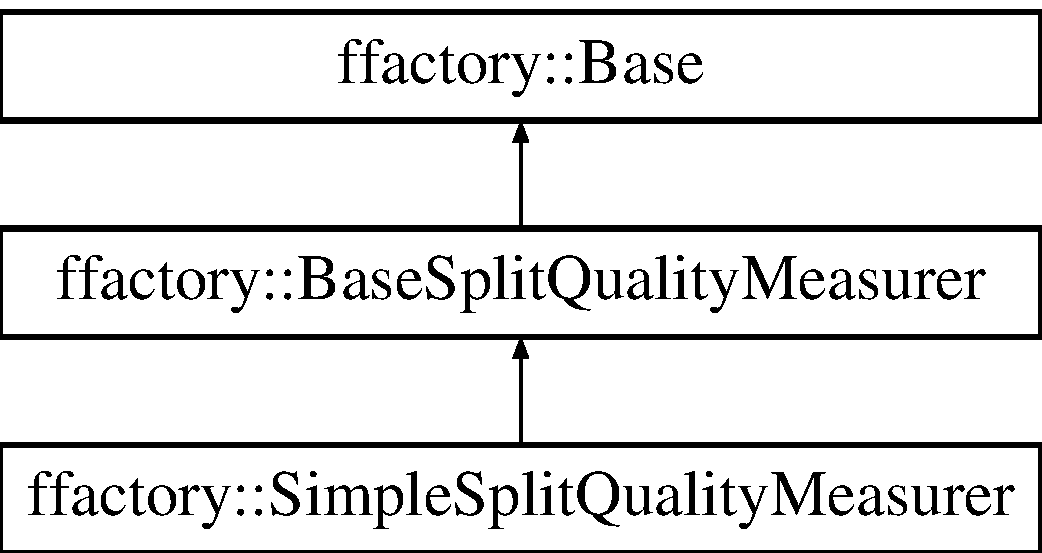
\includegraphics[height=3.000000cm]{classffactory_1_1_base_split_quality_measurer}
\end{center}
\end{figure}
\subsection*{Public Member Functions}
\begin{DoxyCompactItemize}
\item 
virtual Data\-Type \hyperlink{classffactory_1_1_base_split_quality_measurer_a64904410d1071ba5aaa6928f0ea7f1a5}{get\-Score} (\hyperlink{classffactory_1_1_partition_statistics}{Partition\-Statistics} $\ast$left, \hyperlink{classffactory_1_1_partition_statistics}{Partition\-Statistics} $\ast$right)=0
\item 
\hypertarget{classffactory_1_1_base_split_quality_measurer_a47054f960d2f5e0a6cba92ac34f38e1f}{\hyperlink{classffactory_1_1_base_impurity_measure}{Base\-Impurity\-Measure} $\ast$ {\bfseries get\-Impurity\-Measure\-Function} ()}\label{classffactory_1_1_base_split_quality_measurer_a47054f960d2f5e0a6cba92ac34f38e1f}

\item 
\hypertarget{classffactory_1_1_base_split_quality_measurer_af4dc1a72248b7c5f3eeca0c805b7488e}{void {\bfseries set\-Impurity\-Measure\-Function} (Base\-Impurity\-Measure\-Unique\-Ptr impurity\-Function)}\label{classffactory_1_1_base_split_quality_measurer_af4dc1a72248b7c5f3eeca0c805b7488e}

\item 
virtual std\-::string \hyperlink{classffactory_1_1_base_split_quality_measurer_a0bd98e9b10ef01211e0839e9a6f22d26}{get\-Info} ()
\end{DoxyCompactItemize}


\subsection{Detailed Description}
Split quality analysis tool 

\subsection{Member Function Documentation}
\hypertarget{classffactory_1_1_base_split_quality_measurer_a0bd98e9b10ef01211e0839e9a6f22d26}{\index{ffactory\-::\-Base\-Split\-Quality\-Measurer@{ffactory\-::\-Base\-Split\-Quality\-Measurer}!get\-Info@{get\-Info}}
\index{get\-Info@{get\-Info}!ffactory::BaseSplitQualityMeasurer@{ffactory\-::\-Base\-Split\-Quality\-Measurer}}
\subsubsection[{get\-Info}]{\setlength{\rightskip}{0pt plus 5cm}virtual std\-::string ffactory\-::\-Base\-Split\-Quality\-Measurer\-::get\-Info (
\begin{DoxyParamCaption}
{}
\end{DoxyParamCaption}
)\hspace{0.3cm}{\ttfamily [inline]}, {\ttfamily [virtual]}}}\label{classffactory_1_1_base_split_quality_measurer_a0bd98e9b10ef01211e0839e9a6f22d26}
Generates information string \begin{DoxyReturn}{Returns}
std\-::string contains information about object 
\end{DoxyReturn}


Reimplemented from \hyperlink{classffactory_1_1_base_a061e6165abeadad3fac626253d14a0c6}{ffactory\-::\-Base}.



Reimplemented in \hyperlink{classffactory_1_1_simple_split_quality_measurer_a2d35a560f2ba91a6be600c8d42f3332e}{ffactory\-::\-Simple\-Split\-Quality\-Measurer}.

\hypertarget{classffactory_1_1_base_split_quality_measurer_a64904410d1071ba5aaa6928f0ea7f1a5}{\index{ffactory\-::\-Base\-Split\-Quality\-Measurer@{ffactory\-::\-Base\-Split\-Quality\-Measurer}!get\-Score@{get\-Score}}
\index{get\-Score@{get\-Score}!ffactory::BaseSplitQualityMeasurer@{ffactory\-::\-Base\-Split\-Quality\-Measurer}}
\subsubsection[{get\-Score}]{\setlength{\rightskip}{0pt plus 5cm}virtual Data\-Type ffactory\-::\-Base\-Split\-Quality\-Measurer\-::get\-Score (
\begin{DoxyParamCaption}
\item[{{\bf Partition\-Statistics} $\ast$}]{left, }
\item[{{\bf Partition\-Statistics} $\ast$}]{right}
\end{DoxyParamCaption}
)\hspace{0.3cm}{\ttfamily [pure virtual]}}}\label{classffactory_1_1_base_split_quality_measurer_a64904410d1071ba5aaa6928f0ea7f1a5}
Obtain split quality based on left and right partition statistics 
\begin{DoxyParams}{Parameters}
{\em left} & \\
\hline
{\em right} & \\
\hline
\end{DoxyParams}
\begin{DoxyReturn}{Returns}

\end{DoxyReturn}


Implemented in \hyperlink{classffactory_1_1_simple_split_quality_measurer_af2c639dd96f8c376f0852ed6e0a2f279}{ffactory\-::\-Simple\-Split\-Quality\-Measurer}.



The documentation for this class was generated from the following file\-:\begin{DoxyCompactItemize}
\item 
src/classifiers/trees/splits/quality\-Measurer/base\-Split\-Quality\-Measurer.\-h\end{DoxyCompactItemize}

\hypertarget{classffactory_1_1_base_stoppage_criterion}{\section{ffactory\-:\-:Base\-Stoppage\-Criterion Class Reference}
\label{classffactory_1_1_base_stoppage_criterion}\index{ffactory\-::\-Base\-Stoppage\-Criterion@{ffactory\-::\-Base\-Stoppage\-Criterion}}
}


{\ttfamily \#include $<$base\-Stoppage\-Criterion.\-h$>$}

Inheritance diagram for ffactory\-:\-:Base\-Stoppage\-Criterion\-:\begin{figure}[H]
\begin{center}
\leavevmode
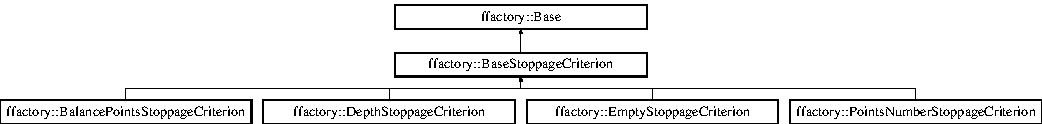
\includegraphics[height=1.666667cm]{classffactory_1_1_base_stoppage_criterion}
\end{center}
\end{figure}
\subsection*{Public Member Functions}
\begin{DoxyCompactItemize}
\item 
virtual bool \hyperlink{classffactory_1_1_base_stoppage_criterion_a47728f0c9b241133e228ea5956248241}{Is\-Stoppage\-Needed} (\hyperlink{classffactory_1_1_base_tree_node}{Base\-Tree\-Node} $\ast$current\-Node, Data\-Vector \&class\-Prob\-Distr)=0
\item 
virtual std\-::string \hyperlink{classffactory_1_1_base_stoppage_criterion_a0543f9c748cb8092e08314a8d2d40c79}{get\-Info} ()
\end{DoxyCompactItemize}


\subsection{Detailed Description}
\hyperlink{classffactory_1_1_base}{Base} class for all stoppage criteria for tree Ru\-:Базовый класс для всех критериев останова 

\subsection{Member Function Documentation}
\hypertarget{classffactory_1_1_base_stoppage_criterion_a0543f9c748cb8092e08314a8d2d40c79}{\index{ffactory\-::\-Base\-Stoppage\-Criterion@{ffactory\-::\-Base\-Stoppage\-Criterion}!get\-Info@{get\-Info}}
\index{get\-Info@{get\-Info}!ffactory::BaseStoppageCriterion@{ffactory\-::\-Base\-Stoppage\-Criterion}}
\subsubsection[{get\-Info}]{\setlength{\rightskip}{0pt plus 5cm}virtual std\-::string ffactory\-::\-Base\-Stoppage\-Criterion\-::get\-Info (
\begin{DoxyParamCaption}
{}
\end{DoxyParamCaption}
)\hspace{0.3cm}{\ttfamily [inline]}, {\ttfamily [virtual]}}}\label{classffactory_1_1_base_stoppage_criterion_a0543f9c748cb8092e08314a8d2d40c79}
Generates information string \begin{DoxyReturn}{Returns}
std\-::string contains information about object 
\end{DoxyReturn}


Reimplemented from \hyperlink{classffactory_1_1_base_a061e6165abeadad3fac626253d14a0c6}{ffactory\-::\-Base}.



Reimplemented in \hyperlink{classffactory_1_1_balance_points_stoppage_criterion_ae5414001f1c98a7fccf961a5015b3aa5}{ffactory\-::\-Balance\-Points\-Stoppage\-Criterion}, \hyperlink{classffactory_1_1_depth_stoppage_criterion_aeb81f88755a7dbae93a176ce8cee5624}{ffactory\-::\-Depth\-Stoppage\-Criterion}, \hyperlink{classffactory_1_1_points_number_stoppage_criterion_af8eaa4b922862c103528d9326115c74f}{ffactory\-::\-Points\-Number\-Stoppage\-Criterion}, and \hyperlink{classffactory_1_1_empty_stoppage_criterion_a19181caac08aad7d05fcc07307c93c70}{ffactory\-::\-Empty\-Stoppage\-Criterion}.

\hypertarget{classffactory_1_1_base_stoppage_criterion_a47728f0c9b241133e228ea5956248241}{\index{ffactory\-::\-Base\-Stoppage\-Criterion@{ffactory\-::\-Base\-Stoppage\-Criterion}!Is\-Stoppage\-Needed@{Is\-Stoppage\-Needed}}
\index{Is\-Stoppage\-Needed@{Is\-Stoppage\-Needed}!ffactory::BaseStoppageCriterion@{ffactory\-::\-Base\-Stoppage\-Criterion}}
\subsubsection[{Is\-Stoppage\-Needed}]{\setlength{\rightskip}{0pt plus 5cm}virtual bool ffactory\-::\-Base\-Stoppage\-Criterion\-::\-Is\-Stoppage\-Needed (
\begin{DoxyParamCaption}
\item[{{\bf Base\-Tree\-Node} $\ast$}]{current\-Node, }
\item[{Data\-Vector \&}]{class\-Prob\-Distr}
\end{DoxyParamCaption}
)\hspace{0.3cm}{\ttfamily [pure virtual]}}}\label{classffactory_1_1_base_stoppage_criterion_a47728f0c9b241133e228ea5956248241}
Stoppage criterion implementation here 
\begin{DoxyParams}{Parameters}
{\em current\-Node} & \\
\hline
{\em class\-Prob\-Distr} & \\
\hline
\end{DoxyParams}
\begin{DoxyReturn}{Returns}

\end{DoxyReturn}


Implemented in \hyperlink{classffactory_1_1_balance_points_stoppage_criterion_ad27450524ea56f2b3925f56014c5ea7d}{ffactory\-::\-Balance\-Points\-Stoppage\-Criterion}, \hyperlink{classffactory_1_1_depth_stoppage_criterion_a363d36a365b10f5d6ad05937c9944ea7}{ffactory\-::\-Depth\-Stoppage\-Criterion}, \hyperlink{classffactory_1_1_points_number_stoppage_criterion_af92444c0b1627a64e82d64f3ee7268d4}{ffactory\-::\-Points\-Number\-Stoppage\-Criterion}, and \hyperlink{classffactory_1_1_empty_stoppage_criterion_a5dca6353a6a813e09c77b53db8e57fd9}{ffactory\-::\-Empty\-Stoppage\-Criterion}.



The documentation for this class was generated from the following file\-:\begin{DoxyCompactItemize}
\item 
src/classifiers/trees/stoppage\-Criteria/base\-Stoppage\-Criterion.\-h\end{DoxyCompactItemize}

\hypertarget{classffactory_1_1_base_tree}{\section{ffactory\-:\-:Base\-Tree Class Reference}
\label{classffactory_1_1_base_tree}\index{ffactory\-::\-Base\-Tree@{ffactory\-::\-Base\-Tree}}
}


{\ttfamily \#include $<$Base\-Tree.\-h$>$}

Inheritance diagram for ffactory\-:\-:Base\-Tree\-:\begin{figure}[H]
\begin{center}
\leavevmode
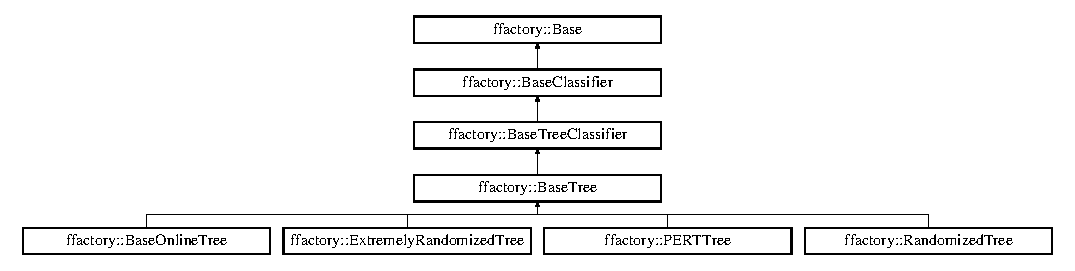
\includegraphics[height=3.196347cm]{classffactory_1_1_base_tree}
\end{center}
\end{figure}
\subsection*{Public Member Functions}
\begin{DoxyCompactItemize}
\item 
\hyperlink{classffactory_1_1_base_tree_node}{Base\-Tree\-Node} $\ast$ \hyperlink{classffactory_1_1_base_tree_a28a8e1d4cf9733ea57af59083d7ee354}{add\-Root} ()
\item 
\hyperlink{classffactory_1_1_base_tree_node}{Base\-Tree\-Node} $\ast$ \hyperlink{classffactory_1_1_base_tree_a3ca64e97f88521e39a706aac4493257f}{add\-Node} (\hyperlink{classffactory_1_1_base_tree_node}{Base\-Tree\-Node} $\ast$parent\-Node, \hyperlink{namespaceffactory_a405b9095f0a093ae4770f7638f0eb730}{Binary\-Tree\-Node\-Type} type)
\item 
\hyperlink{classffactory_1_1_base_tree_node}{Base\-Tree\-Node} $\ast$ \hyperlink{classffactory_1_1_base_tree_ad2921574143761edc31911d530556700}{get\-Node\-By\-Id} (Index\-Type id)
\item 
virtual double \hyperlink{classffactory_1_1_base_tree_ad93e4fb475d3159a378b5148b127a58a}{train} (\hyperlink{classffactory_1_1_dataset}{Dataset} $\ast$d)
\item 
\hyperlink{classffactory_1_1_base_tree_node}{Base\-Tree\-Node} $\ast$ \hyperlink{classffactory_1_1_base_tree_a1ace4078f8e6ac07ef00303a0abde23a}{learn} (\hyperlink{classffactory_1_1_base_tree_node}{Base\-Tree\-Node} $\ast$new\-Node)
\item 
virtual Data\-Vector\-Unique\-Ptr \hyperlink{classffactory_1_1_base_tree_a962907c4083f23175550bf82059d35f0}{predict\-Class\-Prob} (\hyperlink{classffactory_1_1_sample}{Sample} $\ast$sample)
\item 
virtual std\-::string \hyperlink{classffactory_1_1_base_tree_a21d7faa1c68bb531522a73c36b10a95c}{get\-Info} ()
\item 
\hypertarget{classffactory_1_1_base_tree_a7159c76721ce11ed8f0e05d57cd19650}{Index\-Type {\bfseries get\-Predicted\-Leaf\-Id} ()}\label{classffactory_1_1_base_tree_a7159c76721ce11ed8f0e05d57cd19650}

\item 
\hypertarget{classffactory_1_1_base_tree_a05887de99f2723512d200f95a9517662}{unsigned int {\bfseries get\-Id\-Counter} () const }\label{classffactory_1_1_base_tree_a05887de99f2723512d200f95a9517662}

\item 
\hypertarget{classffactory_1_1_base_tree_a32b114258f2a338748626a0dfdfa3769}{void {\bfseries set\-Id\-Counter} (unsigned int id\-Counter)}\label{classffactory_1_1_base_tree_a32b114258f2a338748626a0dfdfa3769}

\item 
\hypertarget{classffactory_1_1_base_tree_a0f805be68fba84631b7f14a35015e4f7}{\hyperlink{classffactory_1_1_base_tree_node}{Base\-Tree\-Node} $\ast$ {\bfseries get\-Root} ()}\label{classffactory_1_1_base_tree_a0f805be68fba84631b7f14a35015e4f7}

\item 
\hypertarget{classffactory_1_1_base_tree_a005a1f829660fd96b5f122489ad4ed97}{void {\bfseries set\-Root} (Base\-Tree\-Node\-Unique\-Ptr root)}\label{classffactory_1_1_base_tree_a005a1f829660fd96b5f122489ad4ed97}

\item 
\hypertarget{classffactory_1_1_base_tree_a6a3451d7304a3a97229d56a531fc9dd5}{\hyperlink{classffactory_1_1_tree_node_factory}{Tree\-Node\-Factory} $\ast$ {\bfseries get\-Node\-Factory} ()}\label{classffactory_1_1_base_tree_a6a3451d7304a3a97229d56a531fc9dd5}

\item 
\hypertarget{classffactory_1_1_base_tree_a1f06198d23a0c51e19b0fa54856869bd}{std\-::string {\bfseries get\-Node\-Type} ()}\label{classffactory_1_1_base_tree_a1f06198d23a0c51e19b0fa54856869bd}

\item 
\hypertarget{classffactory_1_1_base_tree_aaeba2efc8bfeb6886c989f5f519739fb}{void {\bfseries set\-Node\-Type} (std\-::string node\-Type)}\label{classffactory_1_1_base_tree_aaeba2efc8bfeb6886c989f5f519739fb}

\end{DoxyCompactItemize}
\subsection*{Protected Member Functions}
\begin{DoxyCompactItemize}
\item 
\hyperlink{classffactory_1_1_base_tree_node}{Base\-Tree\-Node} $\ast$ \hyperlink{classffactory_1_1_base_tree_a945b1bea9f210079c6688ec5a0c87018}{get\-Tree\-Node\-By\-Id} (\hyperlink{classffactory_1_1_base_tree_node}{Base\-Tree\-Node} $\ast$First\-Node, Index\-Type id)
\end{DoxyCompactItemize}
\subsection*{Protected Attributes}
\begin{DoxyCompactItemize}
\item 
\hypertarget{classffactory_1_1_base_tree_a8a5d418c6bddeee0a4495dadaf6b8136}{Base\-Tree\-Node\-Unique\-Ptr {\bfseries Root}}\label{classffactory_1_1_base_tree_a8a5d418c6bddeee0a4495dadaf6b8136}

\item 
\hypertarget{classffactory_1_1_base_tree_af31f1583719f797c6c8bbf1c1c82050b}{\hyperlink{classffactory_1_1_tree_node_factory}{Tree\-Node\-Factory} {\bfseries node\-Factory}}\label{classffactory_1_1_base_tree_af31f1583719f797c6c8bbf1c1c82050b}

\item 
\hypertarget{classffactory_1_1_base_tree_a6d076f850764b5707baa35cdc4c0a8ca}{std\-::string {\bfseries node\-Type}}\label{classffactory_1_1_base_tree_a6d076f850764b5707baa35cdc4c0a8ca}

\item 
\hypertarget{classffactory_1_1_base_tree_a505141e97bcfffde60679169405937e3}{Index\-Type {\bfseries id\-Counter}}\label{classffactory_1_1_base_tree_a505141e97bcfffde60679169405937e3}

\item 
\hypertarget{classffactory_1_1_base_tree_a8678b16b0abe5ea9106c72ed5310e202}{Index\-Type {\bfseries predicted\-Leaf\-Id}}\label{classffactory_1_1_base_tree_a8678b16b0abe5ea9106c72ed5310e202}

\end{DoxyCompactItemize}


\subsection{Detailed Description}
\hyperlink{classffactory_1_1_base}{Base} class for all (binary) trees 

\subsection{Member Function Documentation}
\hypertarget{classffactory_1_1_base_tree_a3ca64e97f88521e39a706aac4493257f}{\index{ffactory\-::\-Base\-Tree@{ffactory\-::\-Base\-Tree}!add\-Node@{add\-Node}}
\index{add\-Node@{add\-Node}!ffactory::BaseTree@{ffactory\-::\-Base\-Tree}}
\subsubsection[{add\-Node}]{\setlength{\rightskip}{0pt plus 5cm}{\bf Base\-Tree\-Node}$\ast$ ffactory\-::\-Base\-Tree\-::add\-Node (
\begin{DoxyParamCaption}
\item[{{\bf Base\-Tree\-Node} $\ast$}]{parent\-Node, }
\item[{{\bf Binary\-Tree\-Node\-Type}}]{type}
\end{DoxyParamCaption}
)\hspace{0.3cm}{\ttfamily [inline]}}}\label{classffactory_1_1_base_tree_a3ca64e97f88521e39a706aac4493257f}
Add {\itshape new\-Node} to right (or left) branch of {\itshape parent\-Node} 
\begin{DoxyParams}{Parameters}
{\em new\-Node} & \\
\hline
{\em parent\-Node} & \\
\hline
{\em to\-Right} & \\
\hline
\end{DoxyParams}
\hypertarget{classffactory_1_1_base_tree_a28a8e1d4cf9733ea57af59083d7ee354}{\index{ffactory\-::\-Base\-Tree@{ffactory\-::\-Base\-Tree}!add\-Root@{add\-Root}}
\index{add\-Root@{add\-Root}!ffactory::BaseTree@{ffactory\-::\-Base\-Tree}}
\subsubsection[{add\-Root}]{\setlength{\rightskip}{0pt plus 5cm}{\bf Base\-Tree\-Node}$\ast$ ffactory\-::\-Base\-Tree\-::add\-Root (
\begin{DoxyParamCaption}
{}
\end{DoxyParamCaption}
)\hspace{0.3cm}{\ttfamily [inline]}}}\label{classffactory_1_1_base_tree_a28a8e1d4cf9733ea57af59083d7ee354}
Create root node \begin{DoxyReturn}{Returns}
pointer to node 
\end{DoxyReturn}
\hypertarget{classffactory_1_1_base_tree_a21d7faa1c68bb531522a73c36b10a95c}{\index{ffactory\-::\-Base\-Tree@{ffactory\-::\-Base\-Tree}!get\-Info@{get\-Info}}
\index{get\-Info@{get\-Info}!ffactory::BaseTree@{ffactory\-::\-Base\-Tree}}
\subsubsection[{get\-Info}]{\setlength{\rightskip}{0pt plus 5cm}virtual std\-::string ffactory\-::\-Base\-Tree\-::get\-Info (
\begin{DoxyParamCaption}
{}
\end{DoxyParamCaption}
)\hspace{0.3cm}{\ttfamily [inline]}, {\ttfamily [virtual]}}}\label{classffactory_1_1_base_tree_a21d7faa1c68bb531522a73c36b10a95c}
Generates information string \begin{DoxyReturn}{Returns}
std\-::string contains information about classifier 
\end{DoxyReturn}
\begin{DoxyRefDesc}{Todo}
\item[\hyperlink{todo__todo000003}{Todo}]Написать вывод полной инфы о дереве \end{DoxyRefDesc}


Reimplemented from \hyperlink{classffactory_1_1_base_classifier_af6b0a89fd34ba70626104500d612d836}{ffactory\-::\-Base\-Classifier}.



Reimplemented in \hyperlink{classffactory_1_1_base_online_tree_ad814d53893b7321f3384677b864ba2de}{ffactory\-::\-Base\-Online\-Tree}.

\hypertarget{classffactory_1_1_base_tree_ad2921574143761edc31911d530556700}{\index{ffactory\-::\-Base\-Tree@{ffactory\-::\-Base\-Tree}!get\-Node\-By\-Id@{get\-Node\-By\-Id}}
\index{get\-Node\-By\-Id@{get\-Node\-By\-Id}!ffactory::BaseTree@{ffactory\-::\-Base\-Tree}}
\subsubsection[{get\-Node\-By\-Id}]{\setlength{\rightskip}{0pt plus 5cm}{\bf Base\-Tree\-Node}$\ast$ ffactory\-::\-Base\-Tree\-::get\-Node\-By\-Id (
\begin{DoxyParamCaption}
\item[{Index\-Type}]{id}
\end{DoxyParamCaption}
)\hspace{0.3cm}{\ttfamily [inline]}}}\label{classffactory_1_1_base_tree_ad2921574143761edc31911d530556700}

\begin{DoxyParams}{Parameters}
{\em id} & \\
\hline
\end{DoxyParams}
\begin{DoxyReturn}{Returns}

\end{DoxyReturn}
\hypertarget{classffactory_1_1_base_tree_a945b1bea9f210079c6688ec5a0c87018}{\index{ffactory\-::\-Base\-Tree@{ffactory\-::\-Base\-Tree}!get\-Tree\-Node\-By\-Id@{get\-Tree\-Node\-By\-Id}}
\index{get\-Tree\-Node\-By\-Id@{get\-Tree\-Node\-By\-Id}!ffactory::BaseTree@{ffactory\-::\-Base\-Tree}}
\subsubsection[{get\-Tree\-Node\-By\-Id}]{\setlength{\rightskip}{0pt plus 5cm}{\bf Base\-Tree\-Node}$\ast$ ffactory\-::\-Base\-Tree\-::get\-Tree\-Node\-By\-Id (
\begin{DoxyParamCaption}
\item[{{\bf Base\-Tree\-Node} $\ast$}]{First\-Node, }
\item[{Index\-Type}]{id}
\end{DoxyParamCaption}
)\hspace{0.3cm}{\ttfamily [inline]}, {\ttfamily [protected]}}}\label{classffactory_1_1_base_tree_a945b1bea9f210079c6688ec5a0c87018}
Get pointer to node with specified {\itshape id} from {\itshape First\-Node} 
\begin{DoxyParams}{Parameters}
{\em First\-Node} & \\
\hline
{\em id} & \\
\hline
\end{DoxyParams}
\begin{DoxyReturn}{Returns}
\hyperlink{classffactory_1_1_base_tree_node}{Base\-Tree\-Node} pointer from Base\-Tree\-Node\-Unique\-Ptr 
\end{DoxyReturn}
\hypertarget{classffactory_1_1_base_tree_a1ace4078f8e6ac07ef00303a0abde23a}{\index{ffactory\-::\-Base\-Tree@{ffactory\-::\-Base\-Tree}!learn@{learn}}
\index{learn@{learn}!ffactory::BaseTree@{ffactory\-::\-Base\-Tree}}
\subsubsection[{learn}]{\setlength{\rightskip}{0pt plus 5cm}{\bf Base\-Tree\-Node}$\ast$ ffactory\-::\-Base\-Tree\-::learn (
\begin{DoxyParamCaption}
\item[{{\bf Base\-Tree\-Node} $\ast$}]{new\-Node}
\end{DoxyParamCaption}
)\hspace{0.3cm}{\ttfamily [inline]}}}\label{classffactory_1_1_base_tree_a1ace4078f8e6ac07ef00303a0abde23a}
Recursive function of tree learning 
\begin{DoxyParams}{Parameters}
{\em new\-Node} & \\
\hline
{\em m} & \\
\hline
\end{DoxyParams}
\begin{DoxyReturn}{Returns}

\end{DoxyReturn}
\hypertarget{classffactory_1_1_base_tree_a962907c4083f23175550bf82059d35f0}{\index{ffactory\-::\-Base\-Tree@{ffactory\-::\-Base\-Tree}!predict\-Class\-Prob@{predict\-Class\-Prob}}
\index{predict\-Class\-Prob@{predict\-Class\-Prob}!ffactory::BaseTree@{ffactory\-::\-Base\-Tree}}
\subsubsection[{predict\-Class\-Prob}]{\setlength{\rightskip}{0pt plus 5cm}virtual Data\-Vector\-Unique\-Ptr ffactory\-::\-Base\-Tree\-::predict\-Class\-Prob (
\begin{DoxyParamCaption}
\item[{{\bf Sample} $\ast$}]{sample}
\end{DoxyParamCaption}
)\hspace{0.3cm}{\ttfamily [inline]}, {\ttfamily [virtual]}}}\label{classffactory_1_1_base_tree_a962907c4083f23175550bf82059d35f0}
Predict class probability of one sample 
\begin{DoxyParams}{Parameters}
{\em sample} & \\
\hline
\end{DoxyParams}
\begin{DoxyReturn}{Returns}
Index of class 
\end{DoxyReturn}


Implements \hyperlink{classffactory_1_1_base_classifier_a6758932ce8f59eeffd0e66404a0332e4}{ffactory\-::\-Base\-Classifier}.

\hypertarget{classffactory_1_1_base_tree_ad93e4fb475d3159a378b5148b127a58a}{\index{ffactory\-::\-Base\-Tree@{ffactory\-::\-Base\-Tree}!train@{train}}
\index{train@{train}!ffactory::BaseTree@{ffactory\-::\-Base\-Tree}}
\subsubsection[{train}]{\setlength{\rightskip}{0pt plus 5cm}virtual double ffactory\-::\-Base\-Tree\-::train (
\begin{DoxyParamCaption}
\item[{{\bf Dataset} $\ast$}]{d}
\end{DoxyParamCaption}
)\hspace{0.3cm}{\ttfamily [inline]}, {\ttfamily [virtual]}}}\label{classffactory_1_1_base_tree_ad93e4fb475d3159a378b5148b127a58a}
Train classifier on dataset {\itshape d} 
\begin{DoxyParams}{Parameters}
{\em d} & \\
\hline
\end{DoxyParams}
\begin{DoxyReturn}{Returns}
Value of specified error measure on dataset {\itshape d} 
\end{DoxyReturn}


Implements \hyperlink{classffactory_1_1_base_classifier_a150000cb5cd9b2bb4380b47f33a462f2}{ffactory\-::\-Base\-Classifier}.



The documentation for this class was generated from the following file\-:\begin{DoxyCompactItemize}
\item 
src/classifiers/trees/Base\-Tree.\-h\end{DoxyCompactItemize}

\hypertarget{classffactory_1_1_base_tree_classifier}{\section{ffactory\-:\-:Base\-Tree\-Classifier Class Reference}
\label{classffactory_1_1_base_tree_classifier}\index{ffactory\-::\-Base\-Tree\-Classifier@{ffactory\-::\-Base\-Tree\-Classifier}}
}


{\ttfamily \#include $<$base\-Tree\-Classifier.\-h$>$}

Inheritance diagram for ffactory\-:\-:Base\-Tree\-Classifier\-:\begin{figure}[H]
\begin{center}
\leavevmode
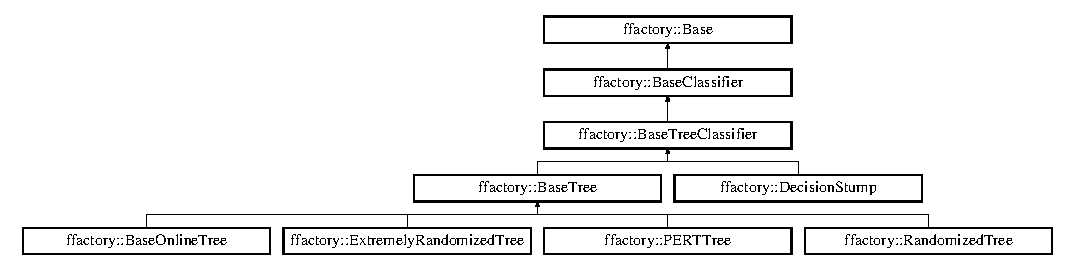
\includegraphics[height=3.196347cm]{classffactory_1_1_base_tree_classifier}
\end{center}
\end{figure}
\subsection*{Public Member Functions}
\begin{DoxyCompactItemize}
\item 
\hypertarget{classffactory_1_1_base_tree_classifier_a247e330e8ce0f78f3036d7fc1a8d1f77}{\hyperlink{classffactory_1_1_base_split_candidate_generator}{Base\-Split\-Candidate\-Generator} $\ast$ {\bfseries get\-Split\-Generator} ()}\label{classffactory_1_1_base_tree_classifier_a247e330e8ce0f78f3036d7fc1a8d1f77}

\item 
\hypertarget{classffactory_1_1_base_tree_classifier_af645d0173a84e1c4b6653ed3b158a591}{void {\bfseries set\-Split\-Generator} (Base\-Split\-Candidate\-Generator\-Unique\-Ptr split\-Generator)}\label{classffactory_1_1_base_tree_classifier_af645d0173a84e1c4b6653ed3b158a591}

\item 
\hypertarget{classffactory_1_1_base_tree_classifier_ac1918fd2d7a54e6158db436d0437aa1b}{\hyperlink{classffactory_1_1_base_split_quality_measurer}{Base\-Split\-Quality\-Measurer} $\ast$ {\bfseries get\-Split\-Quality\-Measurer} ()}\label{classffactory_1_1_base_tree_classifier_ac1918fd2d7a54e6158db436d0437aa1b}

\item 
\hypertarget{classffactory_1_1_base_tree_classifier_a35b137b7c73418168c8cd643602ee920}{void {\bfseries set\-Split\-Quality\-Measurer} (Base\-Split\-Quality\-Measurer\-Unique\-Ptr split\-Quality\-Measurer)}\label{classffactory_1_1_base_tree_classifier_a35b137b7c73418168c8cd643602ee920}

\item 
\hypertarget{classffactory_1_1_base_tree_classifier_ab4ee8d40db7e78c11d4dc69a613ffbaa}{\hyperlink{classffactory_1_1_base_stoppage_criterion}{Base\-Stoppage\-Criterion} $\ast$ {\bfseries get\-Stoppage\-Criterion} ()}\label{classffactory_1_1_base_tree_classifier_ab4ee8d40db7e78c11d4dc69a613ffbaa}

\item 
\hypertarget{classffactory_1_1_base_tree_classifier_a1437f2fa8542f814827abc73c92c8f26}{void {\bfseries set\-Stoppage\-Criterion} (Base\-Stoppage\-Criterion\-Unique\-Ptr stoppage\-Criterion)}\label{classffactory_1_1_base_tree_classifier_a1437f2fa8542f814827abc73c92c8f26}

\item 
void \hyperlink{classffactory_1_1_base_tree_classifier_aaf2902effacd5f8c3ea74d80d52d2922}{check\-Settings} ()
\item 
Partition\-Statistics\-Unique\-Ptr \hyperlink{classffactory_1_1_base_tree_classifier_a2e74c97ec3e034a521b75596fe0d6724}{make\-Partitioning\-Stats} (\hyperlink{classffactory_1_1_partition_statistics}{Partition\-Statistics} $\ast$const partition, \hyperlink{classffactory_1_1_binary_split}{Binary\-Split} $\ast$const \hyperlink{namespaceffactory_a1fec00d28dbea621e480fd9f221d972e}{split}, \hyperlink{namespaceffactory_a405b9095f0a093ae4770f7638f0eb730}{Binary\-Tree\-Node\-Type} const type)
\end{DoxyCompactItemize}
\subsection*{Protected Member Functions}
\begin{DoxyCompactItemize}
\item 
void \hyperlink{classffactory_1_1_base_tree_classifier_afa7b131c6d2d3f27b9b79c32f8f9d81e}{make\-Split\-Ranges} (\hyperlink{classffactory_1_1_data_ranges}{Data\-Ranges} $\ast$old\-Ranges, \hyperlink{classffactory_1_1_binary_split}{Binary\-Split} $\ast$const \hyperlink{namespaceffactory_a1fec00d28dbea621e480fd9f221d972e}{split}, \hyperlink{namespaceffactory_a405b9095f0a093ae4770f7638f0eb730}{Binary\-Tree\-Node\-Type} const type)
\end{DoxyCompactItemize}


\subsection{Detailed Description}
\hyperlink{classffactory_1_1_base}{Base} tree classifier class 

\subsection{Member Function Documentation}
\hypertarget{classffactory_1_1_base_tree_classifier_aaf2902effacd5f8c3ea74d80d52d2922}{\index{ffactory\-::\-Base\-Tree\-Classifier@{ffactory\-::\-Base\-Tree\-Classifier}!check\-Settings@{check\-Settings}}
\index{check\-Settings@{check\-Settings}!ffactory::BaseTreeClassifier@{ffactory\-::\-Base\-Tree\-Classifier}}
\subsubsection[{check\-Settings}]{\setlength{\rightskip}{0pt plus 5cm}void ffactory\-::\-Base\-Tree\-Classifier\-::check\-Settings (
\begin{DoxyParamCaption}
{}
\end{DoxyParamCaption}
)\hspace{0.3cm}{\ttfamily [inline]}}}\label{classffactory_1_1_base_tree_classifier_aaf2902effacd5f8c3ea74d80d52d2922}
Check if all required variables were set. \hypertarget{classffactory_1_1_base_tree_classifier_a2e74c97ec3e034a521b75596fe0d6724}{\index{ffactory\-::\-Base\-Tree\-Classifier@{ffactory\-::\-Base\-Tree\-Classifier}!make\-Partitioning\-Stats@{make\-Partitioning\-Stats}}
\index{make\-Partitioning\-Stats@{make\-Partitioning\-Stats}!ffactory::BaseTreeClassifier@{ffactory\-::\-Base\-Tree\-Classifier}}
\subsubsection[{make\-Partitioning\-Stats}]{\setlength{\rightskip}{0pt plus 5cm}Partition\-Statistics\-Unique\-Ptr ffactory\-::\-Base\-Tree\-Classifier\-::make\-Partitioning\-Stats (
\begin{DoxyParamCaption}
\item[{{\bf Partition\-Statistics} $\ast$const}]{partition, }
\item[{{\bf Binary\-Split} $\ast$const}]{split, }
\item[{{\bf Binary\-Tree\-Node\-Type} const}]{type}
\end{DoxyParamCaption}
)\hspace{0.3cm}{\ttfamily [inline]}}}\label{classffactory_1_1_base_tree_classifier_a2e74c97ec3e034a521b75596fe0d6724}
Generate two space partitions {\itshape left} and {\itshape right} produced by splitting using {\itshape split} adherence to {\itshape old\-Ranges} 
\begin{DoxyParams}{Parameters}
{\em old\-Ranges} & \\
\hline
{\em split} & \\
\hline
{\em left} & \\
\hline
{\em right} & \\
\hline
\end{DoxyParams}
\hypertarget{classffactory_1_1_base_tree_classifier_afa7b131c6d2d3f27b9b79c32f8f9d81e}{\index{ffactory\-::\-Base\-Tree\-Classifier@{ffactory\-::\-Base\-Tree\-Classifier}!make\-Split\-Ranges@{make\-Split\-Ranges}}
\index{make\-Split\-Ranges@{make\-Split\-Ranges}!ffactory::BaseTreeClassifier@{ffactory\-::\-Base\-Tree\-Classifier}}
\subsubsection[{make\-Split\-Ranges}]{\setlength{\rightskip}{0pt plus 5cm}void ffactory\-::\-Base\-Tree\-Classifier\-::make\-Split\-Ranges (
\begin{DoxyParamCaption}
\item[{{\bf Data\-Ranges} $\ast$}]{old\-Ranges, }
\item[{{\bf Binary\-Split} $\ast$const}]{split, }
\item[{{\bf Binary\-Tree\-Node\-Type} const}]{type}
\end{DoxyParamCaption}
)\hspace{0.3cm}{\ttfamily [inline]}, {\ttfamily [protected]}}}\label{classffactory_1_1_base_tree_classifier_afa7b131c6d2d3f27b9b79c32f8f9d81e}
Generates left/right splitting ranges 
\begin{DoxyParams}{Parameters}
{\em old\-Ranges} & \\
\hline
{\em split} & \\
\hline
{\em type} & \\
\hline
\end{DoxyParams}


The documentation for this class was generated from the following file\-:\begin{DoxyCompactItemize}
\item 
src/classifiers/trees/base\-Tree\-Classifier.\-h\end{DoxyCompactItemize}

\hypertarget{classffactory_1_1_base_tree_exporter}{\section{ffactory\-:\-:Base\-Tree\-Exporter Class Reference}
\label{classffactory_1_1_base_tree_exporter}\index{ffactory\-::\-Base\-Tree\-Exporter@{ffactory\-::\-Base\-Tree\-Exporter}}
}
Inheritance diagram for ffactory\-:\-:Base\-Tree\-Exporter\-:\begin{figure}[H]
\begin{center}
\leavevmode
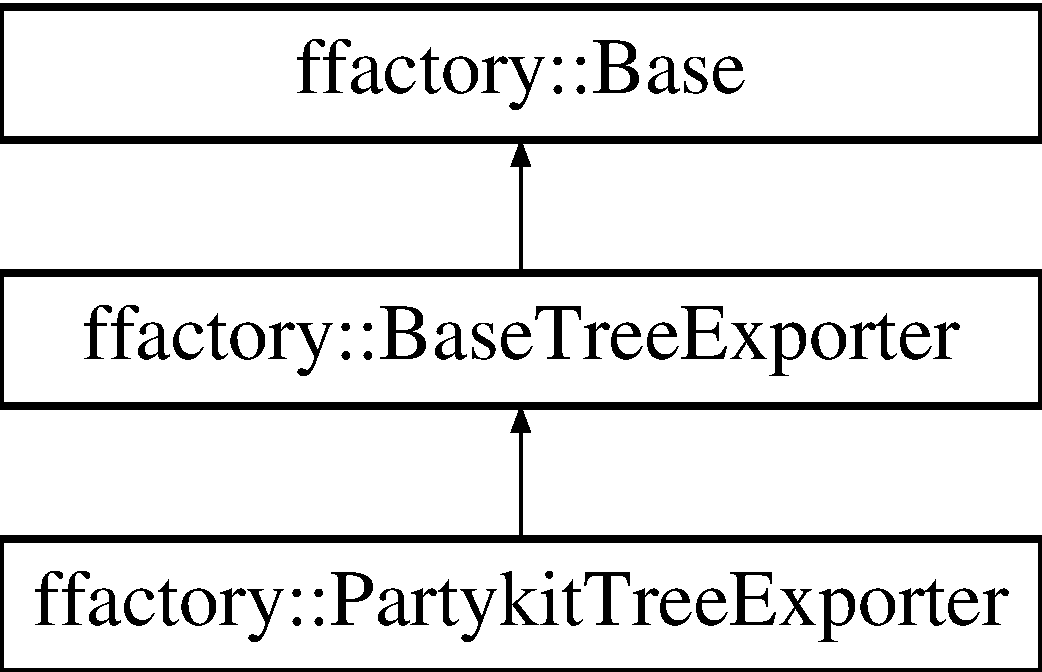
\includegraphics[height=3.000000cm]{classffactory_1_1_base_tree_exporter}
\end{center}
\end{figure}
\subsection*{Public Member Functions}
\begin{DoxyCompactItemize}
\item 
\hypertarget{classffactory_1_1_base_tree_exporter_ae2915d56c4b1da44cd610d205e20a4b4}{std\-::string {\bfseries get\-Filename} ()}\label{classffactory_1_1_base_tree_exporter_ae2915d56c4b1da44cd610d205e20a4b4}

\item 
\hypertarget{classffactory_1_1_base_tree_exporter_ad24336364f470e15670b823daf4e00a9}{void {\bfseries set\-Filename} (std\-::string \&filename)}\label{classffactory_1_1_base_tree_exporter_ad24336364f470e15670b823daf4e00a9}

\item 
\hypertarget{classffactory_1_1_base_tree_exporter_a94b7d461624b417a6955472e5d9304fc}{\hyperlink{classffactory_1_1_base_tree}{Base\-Tree} $\ast$ {\bfseries get\-Tree} ()}\label{classffactory_1_1_base_tree_exporter_a94b7d461624b417a6955472e5d9304fc}

\item 
\hypertarget{classffactory_1_1_base_tree_exporter_a05b3479434f4c27f7e462a06aec99e3d}{void {\bfseries set\-Tree} (\hyperlink{classffactory_1_1_base_tree}{Base\-Tree} $\ast$tree)}\label{classffactory_1_1_base_tree_exporter_a05b3479434f4c27f7e462a06aec99e3d}

\item 
\hypertarget{classffactory_1_1_base_tree_exporter_a7ce46289b3e47e85cb43e9ff4e5d65fc}{virtual void {\bfseries Export} ()=0}\label{classffactory_1_1_base_tree_exporter_a7ce46289b3e47e85cb43e9ff4e5d65fc}

\end{DoxyCompactItemize}


The documentation for this class was generated from the following file\-:\begin{DoxyCompactItemize}
\item 
src/classifiers/trees/export/Base\-Tree\-Exporter.\-h\end{DoxyCompactItemize}

\hypertarget{classffactory_1_1_base_tree_node}{\section{ffactory\-:\-:Base\-Tree\-Node Class Reference}
\label{classffactory_1_1_base_tree_node}\index{ffactory\-::\-Base\-Tree\-Node@{ffactory\-::\-Base\-Tree\-Node}}
}


{\ttfamily \#include $<$base\-Tree\-Node.\-h$>$}

Inheritance diagram for ffactory\-:\-:Base\-Tree\-Node\-:\begin{figure}[H]
\begin{center}
\leavevmode
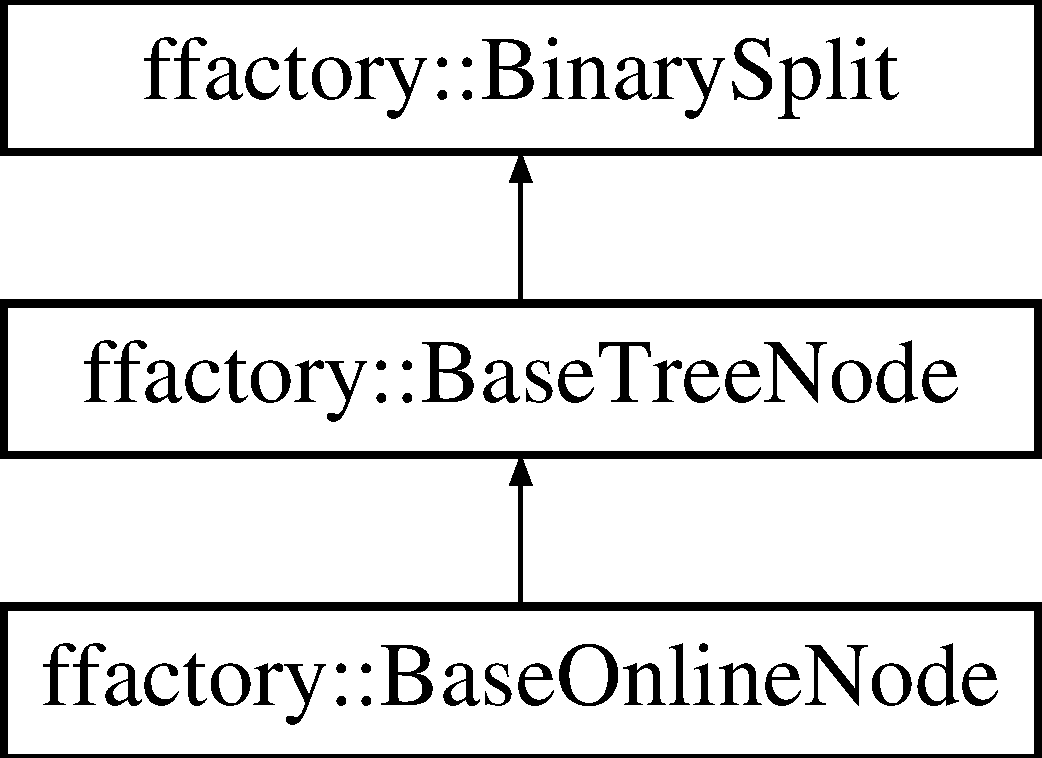
\includegraphics[height=3.000000cm]{classffactory_1_1_base_tree_node}
\end{center}
\end{figure}
\subsection*{Public Member Functions}
\begin{DoxyCompactItemize}
\item 
\hypertarget{classffactory_1_1_base_tree_node_af0ba46cf4d584c0861339177ff50cf0e}{{\bfseries Base\-Tree\-Node} (Index\-Type Node\-Id=0)}\label{classffactory_1_1_base_tree_node_af0ba46cf4d584c0861339177ff50cf0e}

\item 
\hypertarget{classffactory_1_1_base_tree_node_a69d88a9446ebf36589a5b42113b542bd}{void {\bfseries add\-Index} (Index\-Type idx)}\label{classffactory_1_1_base_tree_node_a69d88a9446ebf36589a5b42113b542bd}

\item 
\hypertarget{classffactory_1_1_base_tree_node_a682c96fda66414e2e066fe53c43e29b1}{void {\bfseries clear\-Indexes} ()}\label{classffactory_1_1_base_tree_node_a682c96fda66414e2e066fe53c43e29b1}

\item 
\hypertarget{classffactory_1_1_base_tree_node_a0756be3b3e5e8478af50224acb6eb671}{Index\-Type {\bfseries get\-Indexes\-Size} ()}\label{classffactory_1_1_base_tree_node_a0756be3b3e5e8478af50224acb6eb671}

\item 
\hypertarget{classffactory_1_1_base_tree_node_a78f78571efc1d5c1d18c40cff37b4261}{std\-::vector$<$ Index\-Type $>$ $\ast$ {\bfseries get\-Indexes} ()}\label{classffactory_1_1_base_tree_node_a78f78571efc1d5c1d18c40cff37b4261}

\item 
\hypertarget{classffactory_1_1_base_tree_node_a995a022d3e6460b7a704d8caeabb579e}{\hyperlink{classffactory_1_1_base_tree_node}{Base\-Tree\-Node} \& {\bfseries operator=} (\hyperlink{classffactory_1_1_binary_split}{Binary\-Split} arg)}\label{classffactory_1_1_base_tree_node_a995a022d3e6460b7a704d8caeabb579e}

\item 
\hypertarget{classffactory_1_1_base_tree_node_a3af8472737fb3a1563b9e33960658efc}{void {\bfseries set\-Statistics} (\hyperlink{classffactory_1_1_partition_statistics}{Partition\-Statistics} \&s)}\label{classffactory_1_1_base_tree_node_a3af8472737fb3a1563b9e33960658efc}

\item 
\hypertarget{classffactory_1_1_base_tree_node_af4fac4b4d98b032c9c9155b49e019e8f}{\hyperlink{classffactory_1_1_partition_statistics}{Partition\-Statistics} $\ast$ {\bfseries get\-Statistics} ()}\label{classffactory_1_1_base_tree_node_af4fac4b4d98b032c9c9155b49e019e8f}

\item 
\hypertarget{classffactory_1_1_base_tree_node_a0c762879b8a4677d53911fe108827317}{void {\bfseries set\-Ranges} (\hyperlink{classffactory_1_1_data_ranges}{Data\-Ranges} $\ast$const dr)}\label{classffactory_1_1_base_tree_node_a0c762879b8a4677d53911fe108827317}

\item 
\hypertarget{classffactory_1_1_base_tree_node_a231b613baa3376d6016ba633e8fa6bd9}{\hyperlink{classffactory_1_1_data_ranges}{Data\-Ranges} $\ast$ {\bfseries get\-Ranges} ()}\label{classffactory_1_1_base_tree_node_a231b613baa3376d6016ba633e8fa6bd9}

\item 
\hypertarget{classffactory_1_1_base_tree_node_ac41ac0ec2e040e9d767e7013f5adb01d}{void {\bfseries attach\-To\-Parent} (\hyperlink{classffactory_1_1_base_tree_node}{Base\-Tree\-Node} $\ast$parent)}\label{classffactory_1_1_base_tree_node_ac41ac0ec2e040e9d767e7013f5adb01d}

\item 
\hypertarget{classffactory_1_1_base_tree_node_ad84c8bc0498c1e818b7659de3d43c5e5}{bool {\bfseries is\-Terminal} ()}\label{classffactory_1_1_base_tree_node_ad84c8bc0498c1e818b7659de3d43c5e5}

\item 
\hypertarget{classffactory_1_1_base_tree_node_a1e999c8c583b3aabd9e87c4dee313a0d}{bool {\bfseries is\-Root} ()}\label{classffactory_1_1_base_tree_node_a1e999c8c583b3aabd9e87c4dee313a0d}

\item 
\hyperlink{namespaceffactory_a405b9095f0a093ae4770f7638f0eb730}{Binary\-Tree\-Node\-Type} \hyperlink{classffactory_1_1_base_tree_node_aedced6bc8f534ed88d9d928b2c3a412d}{get\-Node\-Type} ()
\item 
\hypertarget{classffactory_1_1_base_tree_node_a34158e8bb82b12cbf6e38ccf88ae3c5e}{\hyperlink{classffactory_1_1_base_tree_node}{Base\-Tree\-Node} $\ast$ {\bfseries get\-Child} (\hyperlink{namespaceffactory_a405b9095f0a093ae4770f7638f0eb730}{Binary\-Tree\-Node\-Type} type)}\label{classffactory_1_1_base_tree_node_a34158e8bb82b12cbf6e38ccf88ae3c5e}

\item 
\hypertarget{classffactory_1_1_base_tree_node_a54b5c7ef160b6758c33b04a28cda3519}{unsigned int {\bfseries get\-Class\-Label} () const }\label{classffactory_1_1_base_tree_node_a54b5c7ef160b6758c33b04a28cda3519}

\item 
\hypertarget{classffactory_1_1_base_tree_node_aa6d79995bbc38cc13fa3c0cde0b0ccf9}{void {\bfseries set\-Class\-Label} (const unsigned int class\-Label)}\label{classffactory_1_1_base_tree_node_aa6d79995bbc38cc13fa3c0cde0b0ccf9}

\item 
\hypertarget{classffactory_1_1_base_tree_node_af82d12191ce62b7eaad4ef642cbbd324}{unsigned int {\bfseries get\-Depth} () const }\label{classffactory_1_1_base_tree_node_af82d12191ce62b7eaad4ef642cbbd324}

\item 
\hypertarget{classffactory_1_1_base_tree_node_a0960fa1f38afea78e2d651d6b81e847b}{void {\bfseries set\-Depth} (const unsigned int depth)}\label{classffactory_1_1_base_tree_node_a0960fa1f38afea78e2d651d6b81e847b}

\item 
\hypertarget{classffactory_1_1_base_tree_node_a217df7799507516a0e6d739b6cce1879}{unsigned int {\bfseries get\-Id} ()}\label{classffactory_1_1_base_tree_node_a217df7799507516a0e6d739b6cce1879}

\item 
\hypertarget{classffactory_1_1_base_tree_node_a2100a0ca38b922a498a3a32d97128cb7}{void {\bfseries set\-Id} (const unsigned int id)}\label{classffactory_1_1_base_tree_node_a2100a0ca38b922a498a3a32d97128cb7}

\item 
\hypertarget{classffactory_1_1_base_tree_node_af48b4a9254c715ae6c24fdf245ead76e}{\hyperlink{classffactory_1_1_base_tree_node}{Base\-Tree\-Node} $\ast$ {\bfseries get\-Up\-Node} ()}\label{classffactory_1_1_base_tree_node_af48b4a9254c715ae6c24fdf245ead76e}

\item 
\hypertarget{classffactory_1_1_base_tree_node_a852652774f851ac0ed7444177e6ca28b}{void {\bfseries set\-Up\-Node} (\hyperlink{classffactory_1_1_base_tree_node}{Base\-Tree\-Node} $\ast$const up\-Node)}\label{classffactory_1_1_base_tree_node_a852652774f851ac0ed7444177e6ca28b}

\item 
\hypertarget{classffactory_1_1_base_tree_node_a66982055b9accdef826bf004b3508dce}{\hyperlink{classffactory_1_1_base_tree_node}{Base\-Tree\-Node} $\ast$ {\bfseries get\-Down\-Node\-Left} ()}\label{classffactory_1_1_base_tree_node_a66982055b9accdef826bf004b3508dce}

\item 
\hypertarget{classffactory_1_1_base_tree_node_a6eee186634dcec4aa3f818788bd6ba96}{void {\bfseries set\-Down\-Node\-Left} (Base\-Tree\-Node\-Unique\-Ptr down\-Node\-Left)}\label{classffactory_1_1_base_tree_node_a6eee186634dcec4aa3f818788bd6ba96}

\item 
\hypertarget{classffactory_1_1_base_tree_node_a0b7ec999a82040fef492ec0ceb55903f}{\hyperlink{classffactory_1_1_base_tree_node}{Base\-Tree\-Node} $\ast$ {\bfseries get\-Down\-Node\-Right} ()}\label{classffactory_1_1_base_tree_node_a0b7ec999a82040fef492ec0ceb55903f}

\item 
\hypertarget{classffactory_1_1_base_tree_node_a1969bb07f5a3026dbdccde31a09855ff}{void {\bfseries set\-Down\-Node\-Right} (Base\-Tree\-Node\-Unique\-Ptr down\-Node\-Right)}\label{classffactory_1_1_base_tree_node_a1969bb07f5a3026dbdccde31a09855ff}

\item 
\hypertarget{classffactory_1_1_base_tree_node_a74514e2de80e29d91bdfd28a81546e42}{unsigned int {\bfseries get\-Num\-Classes} ()}\label{classffactory_1_1_base_tree_node_a74514e2de80e29d91bdfd28a81546e42}

\item 
\hypertarget{classffactory_1_1_base_tree_node_aa4fbb85a80728e3b37e3744b682e289c}{void {\bfseries set\-Num\-Classes} (unsigned int num\-Classes)}\label{classffactory_1_1_base_tree_node_aa4fbb85a80728e3b37e3744b682e289c}

\item 
\hypertarget{classffactory_1_1_base_tree_node_a0481a1cbd3d67cfa46fdd0756868b4e8}{unsigned int {\bfseries get\-Num\-Features} ()}\label{classffactory_1_1_base_tree_node_a0481a1cbd3d67cfa46fdd0756868b4e8}

\item 
\hypertarget{classffactory_1_1_base_tree_node_a67284d39d4bb9c587234e82e132402ee}{void {\bfseries set\-Num\-Features} (unsigned int num\-Features)}\label{classffactory_1_1_base_tree_node_a67284d39d4bb9c587234e82e132402ee}

\item 
Index\-Type \hyperlink{classffactory_1_1_base_tree_node_ab936c2d3ef94c6c3422f8fd488bcbce3}{compute\-Label} ()
\end{DoxyCompactItemize}


\subsection{Detailed Description}
\hyperlink{classffactory_1_1_base}{Base} data structure for containing of decision tree node information 

\subsection{Member Function Documentation}
\hypertarget{classffactory_1_1_base_tree_node_ab936c2d3ef94c6c3422f8fd488bcbce3}{\index{ffactory\-::\-Base\-Tree\-Node@{ffactory\-::\-Base\-Tree\-Node}!compute\-Label@{compute\-Label}}
\index{compute\-Label@{compute\-Label}!ffactory::BaseTreeNode@{ffactory\-::\-Base\-Tree\-Node}}
\subsubsection[{compute\-Label}]{\setlength{\rightskip}{0pt plus 5cm}Index\-Type ffactory\-::\-Base\-Tree\-Node\-::compute\-Label (
\begin{DoxyParamCaption}
{}
\end{DoxyParamCaption}
)\hspace{0.3cm}{\ttfamily [inline]}}}\label{classffactory_1_1_base_tree_node_ab936c2d3ef94c6c3422f8fd488bcbce3}
Get major class and set label \begin{DoxyReturn}{Returns}

\end{DoxyReturn}
\hypertarget{classffactory_1_1_base_tree_node_aedced6bc8f534ed88d9d928b2c3a412d}{\index{ffactory\-::\-Base\-Tree\-Node@{ffactory\-::\-Base\-Tree\-Node}!get\-Node\-Type@{get\-Node\-Type}}
\index{get\-Node\-Type@{get\-Node\-Type}!ffactory::BaseTreeNode@{ffactory\-::\-Base\-Tree\-Node}}
\subsubsection[{get\-Node\-Type}]{\setlength{\rightskip}{0pt plus 5cm}{\bf Binary\-Tree\-Node\-Type} ffactory\-::\-Base\-Tree\-Node\-::get\-Node\-Type (
\begin{DoxyParamCaption}
{}
\end{DoxyParamCaption}
)\hspace{0.3cm}{\ttfamily [inline]}}}\label{classffactory_1_1_base_tree_node_aedced6bc8f534ed88d9d928b2c3a412d}
\begin{DoxyReturn}{Returns}
Binary\-Tree\-Node\-Type 
\end{DoxyReturn}


The documentation for this class was generated from the following file\-:\begin{DoxyCompactItemize}
\item 
src/classifiers/trees/base\-Tree\-Node.\-h\end{DoxyCompactItemize}

\hypertarget{classffactory_1_1_binary_eigen_file_reader}{\section{ffactory\-:\-:Binary\-Eigen\-File\-Reader Class Reference}
\label{classffactory_1_1_binary_eigen_file_reader}\index{ffactory\-::\-Binary\-Eigen\-File\-Reader@{ffactory\-::\-Binary\-Eigen\-File\-Reader}}
}
Inheritance diagram for ffactory\-:\-:Binary\-Eigen\-File\-Reader\-:\begin{figure}[H]
\begin{center}
\leavevmode
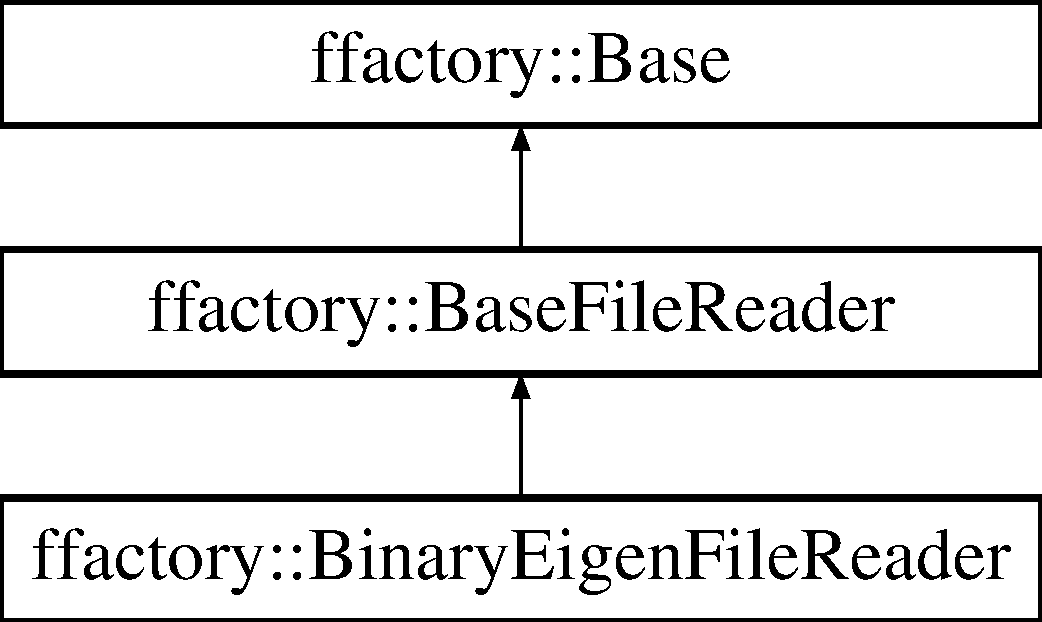
\includegraphics[height=3.000000cm]{classffactory_1_1_binary_eigen_file_reader}
\end{center}
\end{figure}
\subsection*{Public Member Functions}
\begin{DoxyCompactItemize}
\item 
virtual void \hyperlink{classffactory_1_1_binary_eigen_file_reader_ab56d0d075f40f5a659b30f66f84811a4}{read} ()
\end{DoxyCompactItemize}
\subsection*{Additional Inherited Members}


\subsection{Member Function Documentation}
\hypertarget{classffactory_1_1_binary_eigen_file_reader_ab56d0d075f40f5a659b30f66f84811a4}{\index{ffactory\-::\-Binary\-Eigen\-File\-Reader@{ffactory\-::\-Binary\-Eigen\-File\-Reader}!read@{read}}
\index{read@{read}!ffactory::BinaryEigenFileReader@{ffactory\-::\-Binary\-Eigen\-File\-Reader}}
\subsubsection[{read}]{\setlength{\rightskip}{0pt plus 5cm}void ffactory\-::\-Binary\-Eigen\-File\-Reader\-::read (
\begin{DoxyParamCaption}
{}
\end{DoxyParamCaption}
)\hspace{0.3cm}{\ttfamily [virtual]}}}\label{classffactory_1_1_binary_eigen_file_reader_ab56d0d075f40f5a659b30f66f84811a4}
Read file method 

Implements \hyperlink{classffactory_1_1_base_file_reader_ab8683144beea50394ec833163d575615}{ffactory\-::\-Base\-File\-Reader}.



The documentation for this class was generated from the following files\-:\begin{DoxyCompactItemize}
\item 
src/data/file\-Formats/Binary\-Eigen\-File\-Reader.\-h\item 
src/data/file\-Formats/Binary\-Eigen\-File\-Reader.\-cpp\end{DoxyCompactItemize}

\hypertarget{classffactory_1_1_binary_eigen_file_writer}{\section{ffactory\-:\-:Binary\-Eigen\-File\-Writer Class Reference}
\label{classffactory_1_1_binary_eigen_file_writer}\index{ffactory\-::\-Binary\-Eigen\-File\-Writer@{ffactory\-::\-Binary\-Eigen\-File\-Writer}}
}
Inheritance diagram for ffactory\-:\-:Binary\-Eigen\-File\-Writer\-:\begin{figure}[H]
\begin{center}
\leavevmode
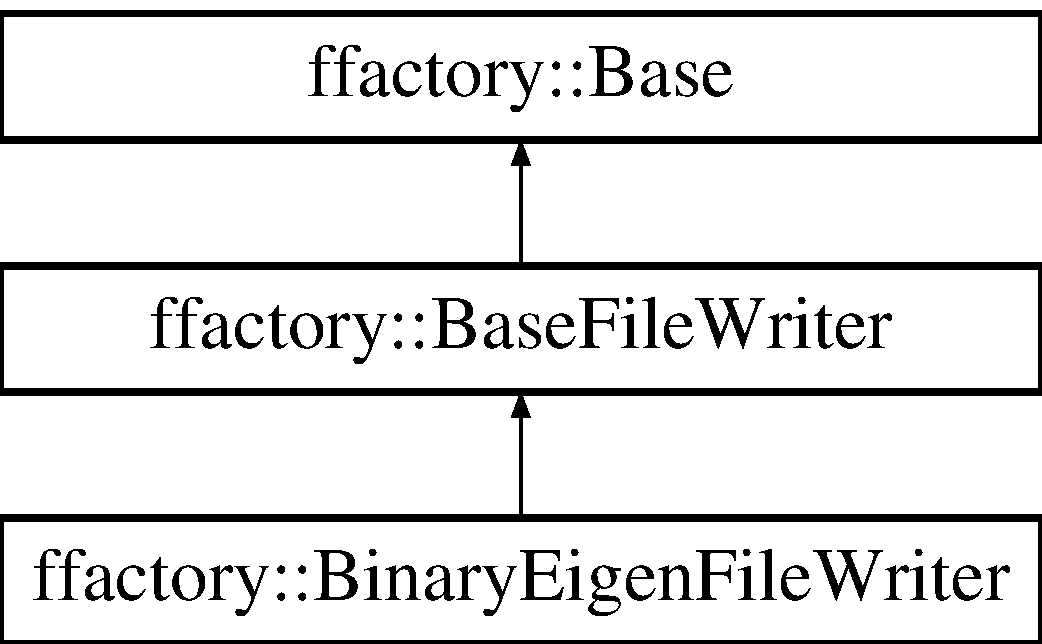
\includegraphics[height=3.000000cm]{classffactory_1_1_binary_eigen_file_writer}
\end{center}
\end{figure}
\subsection*{Public Member Functions}
\begin{DoxyCompactItemize}
\item 
virtual void \hyperlink{classffactory_1_1_binary_eigen_file_writer_a3c9cad431a2149b12e3842223b1e8b19}{write} ()
\end{DoxyCompactItemize}
\subsection*{Additional Inherited Members}


\subsection{Member Function Documentation}
\hypertarget{classffactory_1_1_binary_eigen_file_writer_a3c9cad431a2149b12e3842223b1e8b19}{\index{ffactory\-::\-Binary\-Eigen\-File\-Writer@{ffactory\-::\-Binary\-Eigen\-File\-Writer}!write@{write}}
\index{write@{write}!ffactory::BinaryEigenFileWriter@{ffactory\-::\-Binary\-Eigen\-File\-Writer}}
\subsubsection[{write}]{\setlength{\rightskip}{0pt plus 5cm}void ffactory\-::\-Binary\-Eigen\-File\-Writer\-::write (
\begin{DoxyParamCaption}
{}
\end{DoxyParamCaption}
)\hspace{0.3cm}{\ttfamily [virtual]}}}\label{classffactory_1_1_binary_eigen_file_writer_a3c9cad431a2149b12e3842223b1e8b19}
Write file abstract method 

Implements \hyperlink{classffactory_1_1_base_file_writer_a0674ebc35d7448fe40abead0057eb572}{ffactory\-::\-Base\-File\-Writer}.



The documentation for this class was generated from the following files\-:\begin{DoxyCompactItemize}
\item 
src/data/file\-Formats/Binary\-Eigen\-File\-Writer.\-h\item 
src/data/file\-Formats/Binary\-Eigen\-File\-Writer.\-cpp\end{DoxyCompactItemize}

\hypertarget{classffactory_1_1_binary_split}{\section{ffactory\-:\-:Binary\-Split Class Reference}
\label{classffactory_1_1_binary_split}\index{ffactory\-::\-Binary\-Split@{ffactory\-::\-Binary\-Split}}
}


{\ttfamily \#include $<$binary\-Split.\-h$>$}

Inheritance diagram for ffactory\-:\-:Binary\-Split\-:\begin{figure}[H]
\begin{center}
\leavevmode
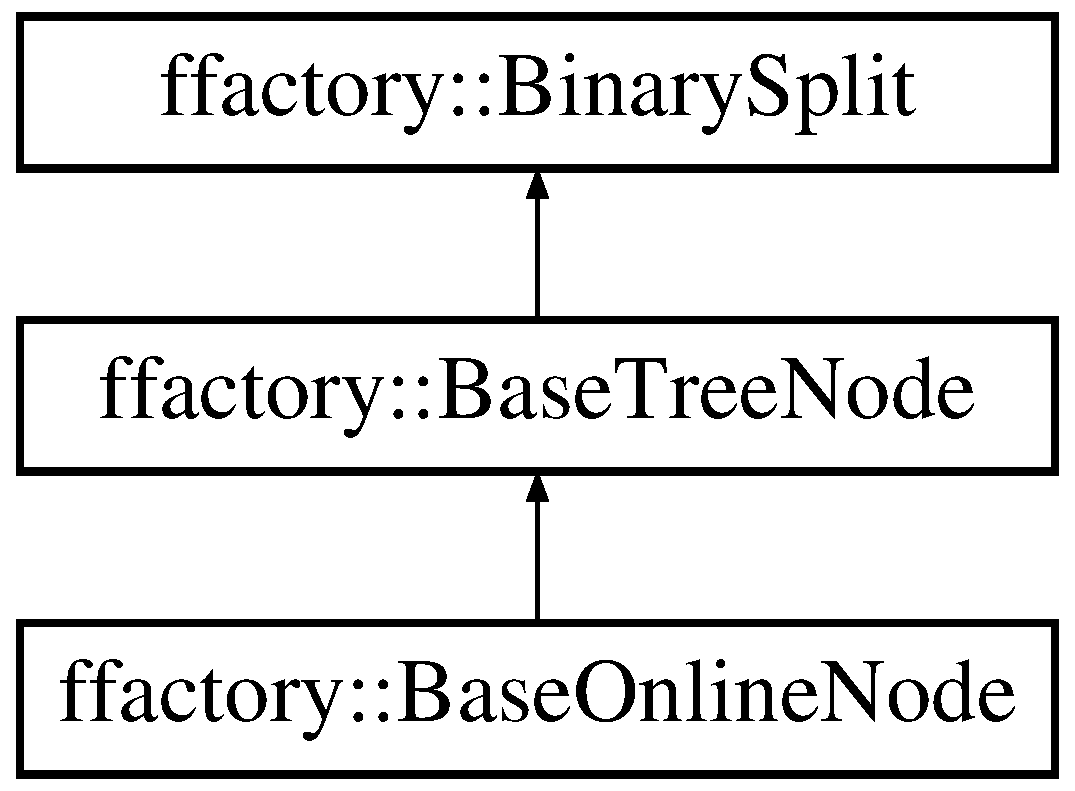
\includegraphics[height=3.000000cm]{classffactory_1_1_binary_split}
\end{center}
\end{figure}
\subsection*{Public Member Functions}
\begin{DoxyCompactItemize}
\item 
\hypertarget{classffactory_1_1_binary_split_a14f42275da38adef19a4e8427f2f0973}{unsigned int {\bfseries get\-Feature\-Index} () const }\label{classffactory_1_1_binary_split_a14f42275da38adef19a4e8427f2f0973}

\item 
\hypertarget{classffactory_1_1_binary_split_a3d43e118b0fde08f33c0afc8fb3e49e1}{void {\bfseries set\-Feature\-Index} (unsigned int feature\-Index)}\label{classffactory_1_1_binary_split_a3d43e118b0fde08f33c0afc8fb3e49e1}

\item 
\hypertarget{classffactory_1_1_binary_split_ae53e23f8dfc47a400948a7fc4bf4efce}{double {\bfseries get\-Feature\-Value} () const }\label{classffactory_1_1_binary_split_ae53e23f8dfc47a400948a7fc4bf4efce}

\item 
\hypertarget{classffactory_1_1_binary_split_a8926e9153314fd9cb1e6503183138143}{void {\bfseries set\-Feature\-Value} (double feature\-Value)}\label{classffactory_1_1_binary_split_a8926e9153314fd9cb1e6503183138143}

\item 
bool \hyperlink{classffactory_1_1_binary_split_a62bca13d9f4e5f796b776125acdc4072}{decide} (Data\-Vector $\ast$feature\-Vector)
\item 
double \hyperlink{classffactory_1_1_binary_split_a5baf70825250efd379c3894567669507}{get\-Score} ()
\item 
void \hyperlink{classffactory_1_1_binary_split_aac5dcfdcf09394dc8f9acf7bd0d74ee6}{set\-Score} (double score)
\item 
\hypertarget{classffactory_1_1_binary_split_ab6a6b527cd16f536d630622b4702b668}{Attribute\-Type {\bfseries get\-Feature\-Type} () const }\label{classffactory_1_1_binary_split_ab6a6b527cd16f536d630622b4702b668}

\item 
\hypertarget{classffactory_1_1_binary_split_a662bb99767628549a0101d8dfd557b5c}{void {\bfseries set\-Feature\-Type} (Attribute\-Type feature\-Type)}\label{classffactory_1_1_binary_split_a662bb99767628549a0101d8dfd557b5c}

\end{DoxyCompactItemize}


\subsection{Detailed Description}
Binary split class propose data structure to store split variable id, value and score calculated by derived classes 

\subsection{Member Function Documentation}
\hypertarget{classffactory_1_1_binary_split_a62bca13d9f4e5f796b776125acdc4072}{\index{ffactory\-::\-Binary\-Split@{ffactory\-::\-Binary\-Split}!decide@{decide}}
\index{decide@{decide}!ffactory::BinarySplit@{ffactory\-::\-Binary\-Split}}
\subsubsection[{decide}]{\setlength{\rightskip}{0pt plus 5cm}bool ffactory\-::\-Binary\-Split\-::decide (
\begin{DoxyParamCaption}
\item[{Data\-Vector $\ast$}]{feature\-Vector}
\end{DoxyParamCaption}
)\hspace{0.3cm}{\ttfamily [inline]}}}\label{classffactory_1_1_binary_split_a62bca13d9f4e5f796b776125acdc4072}
Function of splitting 
\begin{DoxyParams}{Parameters}
{\em feature\-Vector} & point values \\
\hline
\end{DoxyParams}
\begin{DoxyReturn}{Returns}
boolean value feature value $>$ split value 
\end{DoxyReturn}
\hypertarget{classffactory_1_1_binary_split_a5baf70825250efd379c3894567669507}{\index{ffactory\-::\-Binary\-Split@{ffactory\-::\-Binary\-Split}!get\-Score@{get\-Score}}
\index{get\-Score@{get\-Score}!ffactory::BinarySplit@{ffactory\-::\-Binary\-Split}}
\subsubsection[{get\-Score}]{\setlength{\rightskip}{0pt plus 5cm}double ffactory\-::\-Binary\-Split\-::get\-Score (
\begin{DoxyParamCaption}
{}
\end{DoxyParamCaption}
)\hspace{0.3cm}{\ttfamily [inline]}}}\label{classffactory_1_1_binary_split_a5baf70825250efd379c3894567669507}
Split quality value. \begin{DoxyReturn}{Returns}
score 
\end{DoxyReturn}
\hypertarget{classffactory_1_1_binary_split_aac5dcfdcf09394dc8f9acf7bd0d74ee6}{\index{ffactory\-::\-Binary\-Split@{ffactory\-::\-Binary\-Split}!set\-Score@{set\-Score}}
\index{set\-Score@{set\-Score}!ffactory::BinarySplit@{ffactory\-::\-Binary\-Split}}
\subsubsection[{set\-Score}]{\setlength{\rightskip}{0pt plus 5cm}void ffactory\-::\-Binary\-Split\-::set\-Score (
\begin{DoxyParamCaption}
\item[{double}]{score}
\end{DoxyParamCaption}
)\hspace{0.3cm}{\ttfamily [inline]}}}\label{classffactory_1_1_binary_split_aac5dcfdcf09394dc8f9acf7bd0d74ee6}
Split quality value. Can be set externally. 
\begin{DoxyParams}{Parameters}
{\em score} & \\
\hline
\end{DoxyParams}


The documentation for this class was generated from the following file\-:\begin{DoxyCompactItemize}
\item 
src/classifiers/trees/splits/binary\-Split.\-h\end{DoxyCompactItemize}

\hypertarget{classffactory_1_1_class_creator}{\section{ffactory\-:\-:Class\-Creator$<$ B\-C, C $>$ Class Template Reference}
\label{classffactory_1_1_class_creator}\index{ffactory\-::\-Class\-Creator$<$ B\-C, C $>$@{ffactory\-::\-Class\-Creator$<$ B\-C, C $>$}}
}


{\ttfamily \#include $<$Abstract\-Factory.\-h$>$}

Inheritance diagram for ffactory\-:\-:Class\-Creator$<$ B\-C, C $>$\-:\begin{figure}[H]
\begin{center}
\leavevmode
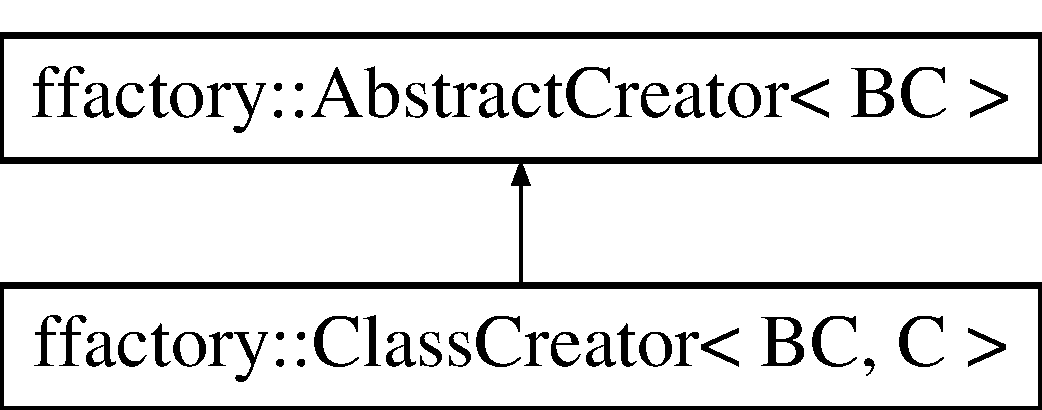
\includegraphics[height=2.000000cm]{classffactory_1_1_class_creator}
\end{center}
\end{figure}
\subsection*{Public Member Functions}
\begin{DoxyCompactItemize}
\item 
\hypertarget{classffactory_1_1_class_creator_a7a8eba0cd42aedc59b7e608085bbf6d7}{virtual C $\ast$ {\bfseries create} ()}\label{classffactory_1_1_class_creator_a7a8eba0cd42aedc59b7e608085bbf6d7}

\end{DoxyCompactItemize}


\subsection{Detailed Description}
\subsubsection*{template$<$class B\-C, class C$>$class ffactory\-::\-Class\-Creator$<$ B\-C, C $>$}

Concrete realization of class-\/creator class for factory pattern (B\-C -\/ base class, C -\/ concrete realization of B\-C) 

The documentation for this class was generated from the following file\-:\begin{DoxyCompactItemize}
\item 
src/utils/patterns/Abstract\-Factory.\-h\end{DoxyCompactItemize}

\hypertarget{classffactory_1_1_csv_file_reader}{\section{ffactory\-:\-:Csv\-File\-Reader Class Reference}
\label{classffactory_1_1_csv_file_reader}\index{ffactory\-::\-Csv\-File\-Reader@{ffactory\-::\-Csv\-File\-Reader}}
}


{\ttfamily \#include $<$Csv\-File\-Reader.\-h$>$}

Inheritance diagram for ffactory\-:\-:Csv\-File\-Reader\-:\begin{figure}[H]
\begin{center}
\leavevmode
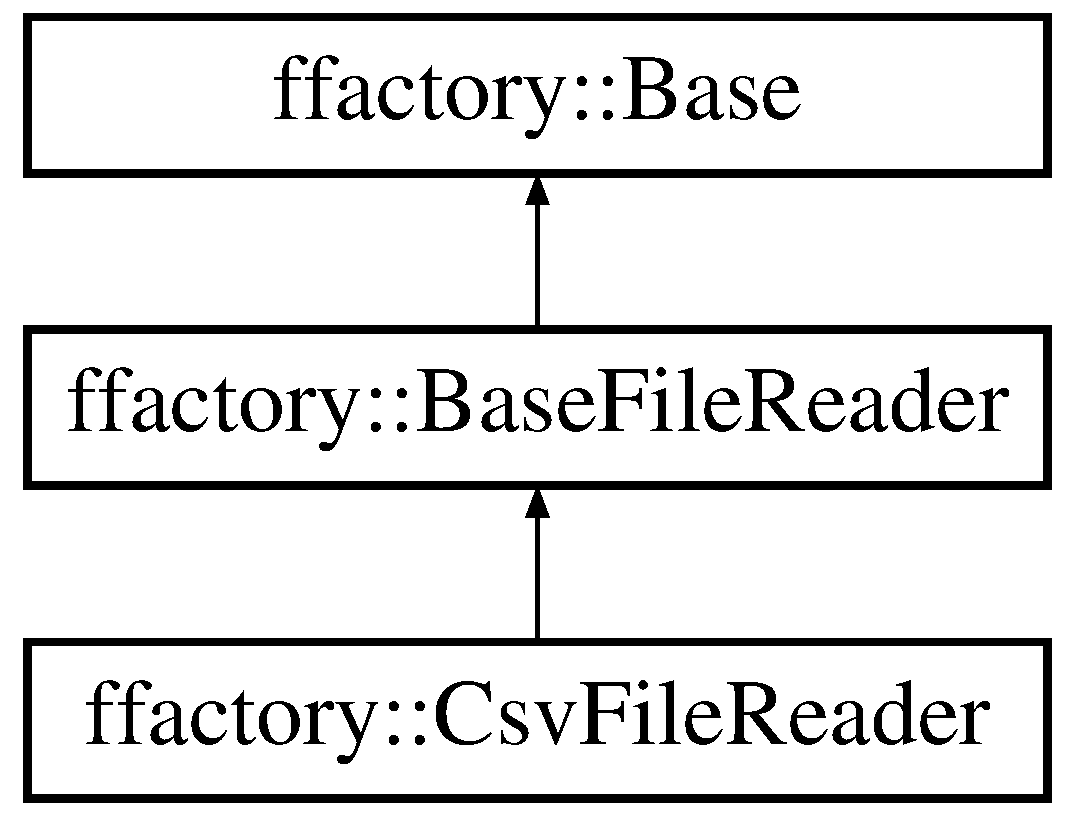
\includegraphics[height=3.000000cm]{classffactory_1_1_csv_file_reader}
\end{center}
\end{figure}
\subsection*{Public Member Functions}
\begin{DoxyCompactItemize}
\item 
virtual void \hyperlink{classffactory_1_1_csv_file_reader_a82882543777400ac3779a89b986a5e98}{read} ()
\item 
\hypertarget{classffactory_1_1_csv_file_reader_a1fa03ef70609068e70834f698ec0eeba}{bool {\bfseries is\-Have\-Header} () const }\label{classffactory_1_1_csv_file_reader_a1fa03ef70609068e70834f698ec0eeba}

\item 
\hypertarget{classffactory_1_1_csv_file_reader_affea39de5d8dbde46828292c6abd5651}{void {\bfseries set\-Have\-Header} (bool have\-Header)}\label{classffactory_1_1_csv_file_reader_affea39de5d8dbde46828292c6abd5651}

\item 
\hypertarget{classffactory_1_1_csv_file_reader_ab95f5d8869771a2bbd334a756d9bbded}{char {\bfseries get\-Delimiter} () const }\label{classffactory_1_1_csv_file_reader_ab95f5d8869771a2bbd334a756d9bbded}

\item 
\hypertarget{classffactory_1_1_csv_file_reader_a626cac1d60076434abaaf87daa52d406}{void {\bfseries set\-Delimiter} (char delimiter)}\label{classffactory_1_1_csv_file_reader_a626cac1d60076434abaaf87daa52d406}

\end{DoxyCompactItemize}
\subsection*{Additional Inherited Members}


\subsection{Detailed Description}
C\-S\-V-\/file support class Restrictions\-: only features columns and one label format, header is required. 

\subsection{Member Function Documentation}
\hypertarget{classffactory_1_1_csv_file_reader_a82882543777400ac3779a89b986a5e98}{\index{ffactory\-::\-Csv\-File\-Reader@{ffactory\-::\-Csv\-File\-Reader}!read@{read}}
\index{read@{read}!ffactory::CsvFileReader@{ffactory\-::\-Csv\-File\-Reader}}
\subsubsection[{read}]{\setlength{\rightskip}{0pt plus 5cm}virtual void ffactory\-::\-Csv\-File\-Reader\-::read (
\begin{DoxyParamCaption}
{}
\end{DoxyParamCaption}
)\hspace{0.3cm}{\ttfamily [inline]}, {\ttfamily [virtual]}}}\label{classffactory_1_1_csv_file_reader_a82882543777400ac3779a89b986a5e98}
Read file abstract method \begin{DoxyRefDesc}{Todo}
\item[\hyperlink{todo__todo000011}{Todo}]Num\-Classes should be set before add \end{DoxyRefDesc}


Implements \hyperlink{classffactory_1_1_base_file_reader_ab8683144beea50394ec833163d575615}{ffactory\-::\-Base\-File\-Reader}.



The documentation for this class was generated from the following file\-:\begin{DoxyCompactItemize}
\item 
src/data/file\-Formats/Csv\-File\-Reader.\-h\end{DoxyCompactItemize}

\hypertarget{classffactory_1_1_csv_file_writer}{\section{ffactory\-:\-:Csv\-File\-Writer Class Reference}
\label{classffactory_1_1_csv_file_writer}\index{ffactory\-::\-Csv\-File\-Writer@{ffactory\-::\-Csv\-File\-Writer}}
}
Inheritance diagram for ffactory\-:\-:Csv\-File\-Writer\-:\begin{figure}[H]
\begin{center}
\leavevmode
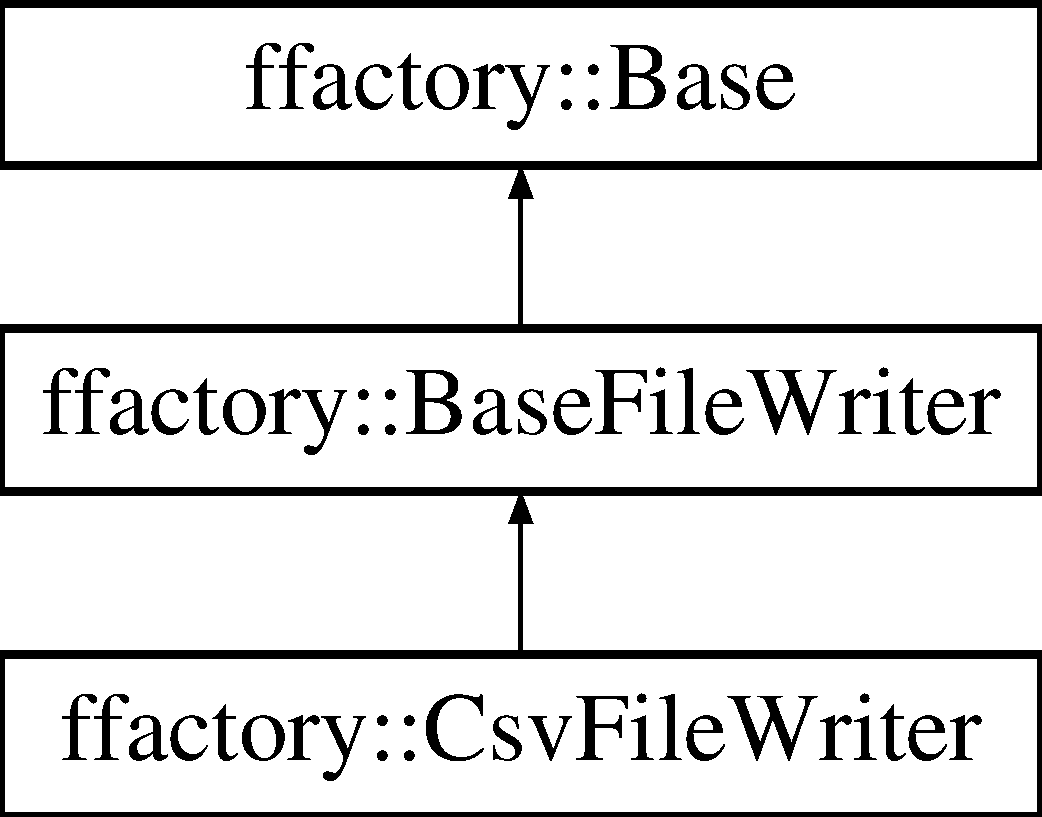
\includegraphics[height=3.000000cm]{classffactory_1_1_csv_file_writer}
\end{center}
\end{figure}
\subsection*{Public Member Functions}
\begin{DoxyCompactItemize}
\item 
virtual void \hyperlink{classffactory_1_1_csv_file_writer_adf8696c5785a68b4a04e2d6f56b047b7}{write} ()
\end{DoxyCompactItemize}
\subsection*{Additional Inherited Members}


\subsection{Member Function Documentation}
\hypertarget{classffactory_1_1_csv_file_writer_adf8696c5785a68b4a04e2d6f56b047b7}{\index{ffactory\-::\-Csv\-File\-Writer@{ffactory\-::\-Csv\-File\-Writer}!write@{write}}
\index{write@{write}!ffactory::CsvFileWriter@{ffactory\-::\-Csv\-File\-Writer}}
\subsubsection[{write}]{\setlength{\rightskip}{0pt plus 5cm}void ffactory\-::\-Csv\-File\-Writer\-::write (
\begin{DoxyParamCaption}
{}
\end{DoxyParamCaption}
)\hspace{0.3cm}{\ttfamily [virtual]}}}\label{classffactory_1_1_csv_file_writer_adf8696c5785a68b4a04e2d6f56b047b7}
Write file abstract method 

Implements \hyperlink{classffactory_1_1_base_file_writer_a0674ebc35d7448fe40abead0057eb572}{ffactory\-::\-Base\-File\-Writer}.



The documentation for this class was generated from the following files\-:\begin{DoxyCompactItemize}
\item 
src/data/file\-Formats/Csv\-File\-Writer.\-h\item 
src/data/file\-Formats/Csv\-File\-Writer.\-cpp\end{DoxyCompactItemize}

\hypertarget{classffactory_1_1_dataloader}{\section{ffactory\-:\-:Dataloader Class Reference}
\label{classffactory_1_1_dataloader}\index{ffactory\-::\-Dataloader@{ffactory\-::\-Dataloader}}
}


{\ttfamily \#include $<$Dataloader.\-h$>$}

Inheritance diagram for ffactory\-:\-:Dataloader\-:\begin{figure}[H]
\begin{center}
\leavevmode
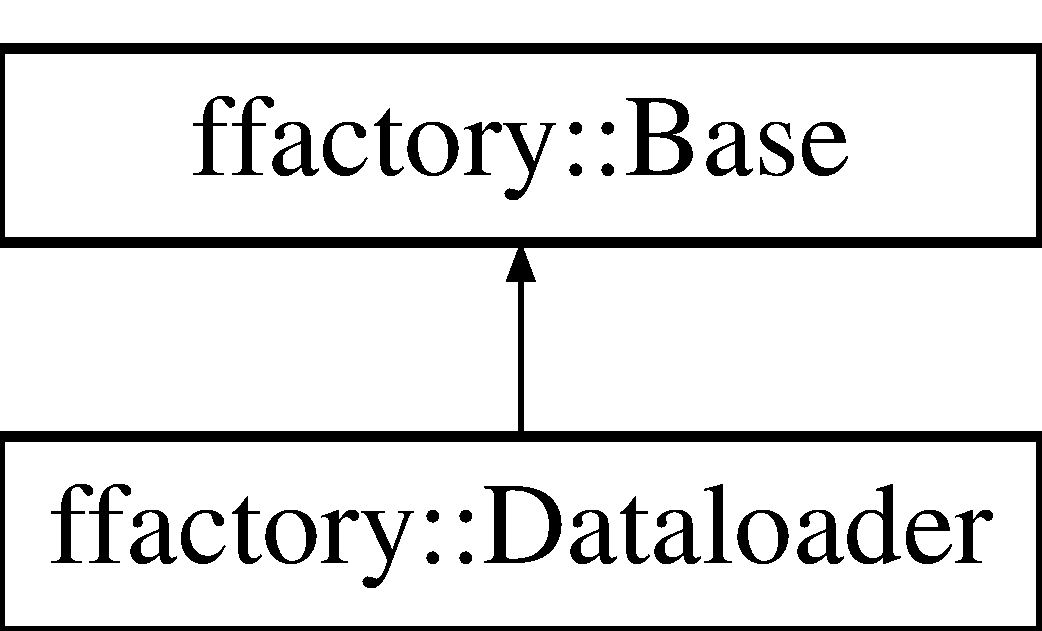
\includegraphics[height=2.000000cm]{classffactory_1_1_dataloader}
\end{center}
\end{figure}
\subsection*{Public Member Functions}
\begin{DoxyCompactItemize}
\item 
\hypertarget{classffactory_1_1_dataloader_a0d89666fe5253f6f9cfa205d7cf1855a}{\hyperlink{classffactory_1_1_dataset}{Dataset} $\ast$ {\bfseries loadcsv} (const std\-::string \&filename)}\label{classffactory_1_1_dataloader_a0d89666fe5253f6f9cfa205d7cf1855a}

\end{DoxyCompactItemize}


\subsection{Detailed Description}
Helps to load data from files (csv supported) 

The documentation for this class was generated from the following file\-:\begin{DoxyCompactItemize}
\item 
src/data/Dataloader.\-h\end{DoxyCompactItemize}

\hypertarget{classffactory_1_1_data_ranges}{\section{ffactory\-:\-:Data\-Ranges Class Reference}
\label{classffactory_1_1_data_ranges}\index{ffactory\-::\-Data\-Ranges@{ffactory\-::\-Data\-Ranges}}
}


{\ttfamily \#include $<$Data\-Ranges.\-h$>$}

\subsection*{Public Member Functions}
\begin{DoxyCompactItemize}
\item 
\hypertarget{classffactory_1_1_data_ranges_a030ee8838df1e3a4739bf17270ad11e3}{{\bfseries Data\-Ranges} (Data\-Vector \&min\-Range\-Vec, Data\-Vector \&max\-Range\-Vec)}\label{classffactory_1_1_data_ranges_a030ee8838df1e3a4739bf17270ad11e3}

\item 
\hypertarget{classffactory_1_1_data_ranges_a7184914acdd43a9d2ec269ba3d7b47e9}{{\bfseries Data\-Ranges} (\hyperlink{classffactory_1_1_data_ranges}{Data\-Ranges} $\ast$dr)}\label{classffactory_1_1_data_ranges_a7184914acdd43a9d2ec269ba3d7b47e9}

\item 
\hypertarget{classffactory_1_1_data_ranges_a6d488ebe76ca0a14b7ff06f1e5de416b}{virtual std\-::string {\bfseries get\-Info} ()}\label{classffactory_1_1_data_ranges_a6d488ebe76ca0a14b7ff06f1e5de416b}

\item 
bool \hyperlink{classffactory_1_1_data_ranges_ac71d2b6b9621948075373cbe90b85422}{is\-Equal} (\hyperlink{classffactory_1_1_data_ranges}{Data\-Ranges} $\ast$dr)
\item 
\hypertarget{classffactory_1_1_data_ranges_a667df88fa397cb1b87ed64c0159fb80e}{bool {\bfseries is\-In\-Ranges\-Exclude\-Greater} (Data\-Vector $\ast$v)}\label{classffactory_1_1_data_ranges_a667df88fa397cb1b87ed64c0159fb80e}

\item 
bool \hyperlink{classffactory_1_1_data_ranges_a7d7c2afc6fc81fa5e32f6b509e6afcfa}{is\-In\-Feature\-Ranges} (Data\-Vector $\ast$v, Index\-Type feature\-Num, bool exclude\-Low\-Bound=true)
\end{DoxyCompactItemize}
\subsection*{Public Attributes}
\begin{DoxyCompactItemize}
\item 
\hypertarget{classffactory_1_1_data_ranges_a6b44ba22ecd2601c42f48faf0657a681}{Data\-Vector {\bfseries min\-Values}}\label{classffactory_1_1_data_ranges_a6b44ba22ecd2601c42f48faf0657a681}

\item 
\hypertarget{classffactory_1_1_data_ranges_ae260ecd84bd0d4ec9b08615f3e3fb067}{Data\-Vector {\bfseries max\-Values}}\label{classffactory_1_1_data_ranges_ae260ecd84bd0d4ec9b08615f3e3fb067}

\end{DoxyCompactItemize}
\subsection*{Friends}
\begin{DoxyCompactItemize}
\item 
\hypertarget{classffactory_1_1_data_ranges_a6f74e94fd009b6d282fc27fd7b604cb0}{std\-::ostream \& {\bfseries operator$<$$<$} (std\-::ostream \&stream, \hyperlink{classffactory_1_1_data_ranges}{Data\-Ranges} \&b)}\label{classffactory_1_1_data_ranges_a6f74e94fd009b6d282fc27fd7b604cb0}

\end{DoxyCompactItemize}


\subsection{Detailed Description}
\hyperlink{classffactory_1_1_data_ranges}{Data\-Ranges} first minimal sample range values second maximal sample range values 

\subsection{Member Function Documentation}
\hypertarget{classffactory_1_1_data_ranges_ac71d2b6b9621948075373cbe90b85422}{\index{ffactory\-::\-Data\-Ranges@{ffactory\-::\-Data\-Ranges}!is\-Equal@{is\-Equal}}
\index{is\-Equal@{is\-Equal}!ffactory::DataRanges@{ffactory\-::\-Data\-Ranges}}
\subsubsection[{is\-Equal}]{\setlength{\rightskip}{0pt plus 5cm}bool ffactory\-::\-Data\-Ranges\-::is\-Equal (
\begin{DoxyParamCaption}
\item[{{\bf Data\-Ranges} $\ast$}]{dr}
\end{DoxyParamCaption}
)\hspace{0.3cm}{\ttfamily [inline]}}}\label{classffactory_1_1_data_ranges_ac71d2b6b9621948075373cbe90b85422}
Check if current data range is equal to {\itshape dr} 
\begin{DoxyParams}{Parameters}
{\em dr} & \\
\hline
\end{DoxyParams}
\begin{DoxyReturn}{Returns}

\end{DoxyReturn}
\hypertarget{classffactory_1_1_data_ranges_a7d7c2afc6fc81fa5e32f6b509e6afcfa}{\index{ffactory\-::\-Data\-Ranges@{ffactory\-::\-Data\-Ranges}!is\-In\-Feature\-Ranges@{is\-In\-Feature\-Ranges}}
\index{is\-In\-Feature\-Ranges@{is\-In\-Feature\-Ranges}!ffactory::DataRanges@{ffactory\-::\-Data\-Ranges}}
\subsubsection[{is\-In\-Feature\-Ranges}]{\setlength{\rightskip}{0pt plus 5cm}bool ffactory\-::\-Data\-Ranges\-::is\-In\-Feature\-Ranges (
\begin{DoxyParamCaption}
\item[{Data\-Vector $\ast$}]{v, }
\item[{Index\-Type}]{feature\-Num, }
\item[{bool}]{exclude\-Low\-Bound = {\ttfamily true}}
\end{DoxyParamCaption}
)\hspace{0.3cm}{\ttfamily [inline]}}}\label{classffactory_1_1_data_ranges_a7d7c2afc6fc81fa5e32f6b509e6afcfa}
Check if point is in specific range (including the values which are equal to range values) P\-L\-E\-S\-E N\-O\-T\-E\-: There're some differences from \hyperlink{classffactory_1_1_partition_statistics_abfc82c4f58a2aac9e1e973f523eb518f}{Partition\-Statistics.\-is\-In\-Ranges} ! 
\begin{DoxyParams}{Parameters}
{\em v} & \\
\hline
{\em feature\-Num} & \\
\hline
{\em exclude\-Low\-Bound} & \\
\hline
\end{DoxyParams}
\begin{DoxyReturn}{Returns}

\end{DoxyReturn}


The documentation for this class was generated from the following file\-:\begin{DoxyCompactItemize}
\item 
src/data/Data\-Ranges.\-h\end{DoxyCompactItemize}

\hypertarget{classffactory_1_1_dataset}{\section{ffactory\-:\-:Dataset Class Reference}
\label{classffactory_1_1_dataset}\index{ffactory\-::\-Dataset@{ffactory\-::\-Dataset}}
}


{\ttfamily \#include $<$Dataset.\-h$>$}

Inheritance diagram for ffactory\-:\-:Dataset\-:\begin{figure}[H]
\begin{center}
\leavevmode
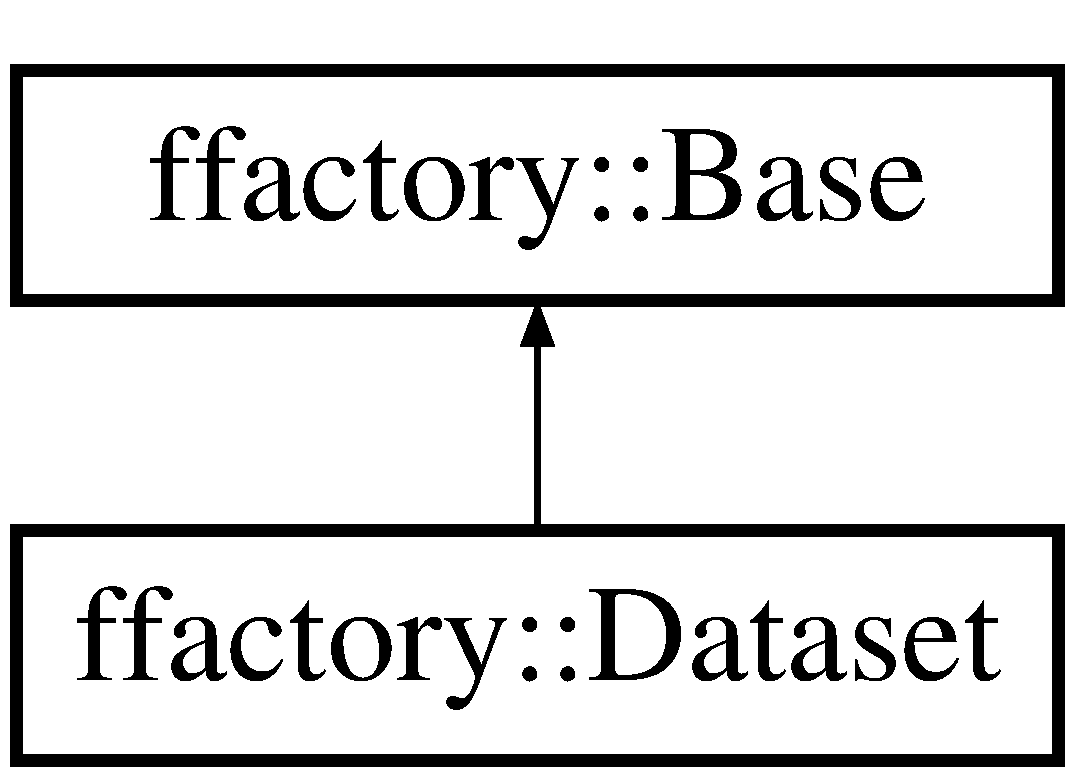
\includegraphics[height=2.000000cm]{classffactory_1_1_dataset}
\end{center}
\end{figure}
\subsection*{Public Member Functions}
\begin{DoxyCompactItemize}
\item 
void \hyperlink{classffactory_1_1_dataset_a199736337b12e0ac97fd36993e00d44b}{set\-Target\-Attribute} (std\-::string name, Attribute\-Type type, String\-Vector $\ast$cat=N\-U\-L\-L)
\item 
void \hyperlink{classffactory_1_1_dataset_aee6bb477f697731452a16dcdfdd634e5}{add\-Attribute} (std\-::string name, Attribute\-Type type, String\-Vector $\ast$cat=N\-U\-L\-L)
\item 
\hypertarget{classffactory_1_1_dataset_aa5f194a2d71d7662df8c94c2f8b18644}{\hyperlink{classffactory_1_1_attribute}{Attribute} $\ast$ {\bfseries get\-Attribute} (Index\-Type index)}\label{classffactory_1_1_dataset_aa5f194a2d71d7662df8c94c2f8b18644}

\item 
Index\-Type \hyperlink{classffactory_1_1_dataset_a4fb9e8d154fab278c89765e979f12cfe}{get\-Attribute\-Index\-By\-Name} (std\-::string name)
\item 
\hypertarget{classffactory_1_1_dataset_a94f784fa41222351ff541847265d964c}{\hyperlink{classffactory_1_1_attribute}{Attribute} $\ast$ {\bfseries get\-Attribute\-By\-Name} (std\-::string name)}\label{classffactory_1_1_dataset_a94f784fa41222351ff541847265d964c}

\item 
\hypertarget{classffactory_1_1_dataset_a2c807fcff912bb178613429f8befb50e}{\hyperlink{classffactory_1_1_partition_statistics}{Partition\-Statistics} $\ast$ {\bfseries get\-Statistics} ()}\label{classffactory_1_1_dataset_a2c807fcff912bb178613429f8befb50e}

\item 
\hypertarget{classffactory_1_1_dataset_a4a3cced96905be07b23ae2a33cbe8a63}{unsigned int {\bfseries get\-Num\-Classes} ()}\label{classffactory_1_1_dataset_a4a3cced96905be07b23ae2a33cbe8a63}

\item 
\hypertarget{classffactory_1_1_dataset_a6ba6095ed22d5cae25ff497d21be1cba}{void {\bfseries init\-Statistics} ()}\label{classffactory_1_1_dataset_a6ba6095ed22d5cae25ff497d21be1cba}

\item 
\hypertarget{classffactory_1_1_dataset_a5bcea50dae4da648a15104e9283a6fce}{void {\bfseries compute\-Statistics} ()}\label{classffactory_1_1_dataset_a5bcea50dae4da648a15104e9283a6fce}

\item 
\hypertarget{classffactory_1_1_dataset_ab850fb87df1ed9916b457cdb32cd1fef}{void {\bfseries set\-Num\-Classes} (unsigned int num\-Classes)}\label{classffactory_1_1_dataset_ab850fb87df1ed9916b457cdb32cd1fef}

\item 
\hypertarget{classffactory_1_1_dataset_ae7e0905c373e08b5ac4d0b6494116113}{unsigned int {\bfseries get\-Num\-Features} ()}\label{classffactory_1_1_dataset_ae7e0905c373e08b5ac4d0b6494116113}

\item 
\hypertarget{classffactory_1_1_dataset_adde747e1d56656c1ab69e74a99c9f5b3}{void {\bfseries set\-Num\-Features} (unsigned int num\-Features)}\label{classffactory_1_1_dataset_adde747e1d56656c1ab69e74a99c9f5b3}

\item 
\hypertarget{classffactory_1_1_dataset_a054cfd19c38faf3ecda47dc2856be301}{unsigned int {\bfseries get\-Num\-Samples} ()}\label{classffactory_1_1_dataset_a054cfd19c38faf3ecda47dc2856be301}

\item 
\hypertarget{classffactory_1_1_dataset_acc9e899186524016f4fc445496cc51e5}{std\-::vector$<$ \hyperlink{classffactory_1_1_sample}{Sample} $>$ $\ast$ {\bfseries get\-Samples} ()}\label{classffactory_1_1_dataset_acc9e899186524016f4fc445496cc51e5}

\item 
void \hyperlink{classffactory_1_1_dataset_ae11f7cb8026bcae1b7213c7e956799c0}{set\-Samples} (std\-::vector$<$ \hyperlink{classffactory_1_1_sample}{Sample} $>$ $\ast$samples)
\item 
\hyperlink{classffactory_1_1_data_ranges}{Data\-Ranges} \hyperlink{classffactory_1_1_dataset_a77c4ab02a3d3c479d0d3ae27543a3f8b}{calculate\-Ranges\-Masked} (Mask\-Vector $\ast$sample\-Mask=N\-U\-L\-L)
\item 
\hypertarget{classffactory_1_1_dataset_a6361c1633c343a831e859ab7b4276e50}{void {\bfseries calculate\-Ranges} ()}\label{classffactory_1_1_dataset_a6361c1633c343a831e859ab7b4276e50}

\item 
void \hyperlink{classffactory_1_1_dataset_a2577ab7582afd11a22b05b0a7b33e470}{clear} ()
\item 
void \hyperlink{classffactory_1_1_dataset_a57862bb9ae4e77f217d1714ba0337d7c}{add} (\hyperlink{classffactory_1_1_sample}{Sample} \&s)
\item 
void \hyperlink{classffactory_1_1_dataset_a02e99a1c9c4a1bc52bda35705414d23f}{remove} (Index\-Type sample\-Idx)
\item 
\hyperlink{classffactory_1_1_sample}{Sample} $\ast$ \hyperlink{classffactory_1_1_dataset_a02aa634dccdde4e814b852b6a9123883}{get\-Sample} (unsigned int i)
\item 
\hyperlink{classffactory_1_1_sample}{Sample} \hyperlink{classffactory_1_1_dataset_a374a6c76e72fb99533cf8fc1c488a3e0}{copy\-Sample} (unsigned int i)
\item 
Data\-Vector $\ast$ \hyperlink{classffactory_1_1_dataset_adc0cba7d6fc2bbf0fa17b639e2dca2bc}{get\-Sample\-Vector} (unsigned int i)
\item 
void \hyperlink{classffactory_1_1_dataset_a4575aa266a4c8fa4358c786a90392cda}{shuffle} ()
\item 
virtual std\-::string \hyperlink{classffactory_1_1_dataset_a3017145c5f83813b81918aa0b2a9679b}{get\-Info} ()
\item 
Dataset\-Unique\-Ptr \hyperlink{classffactory_1_1_dataset_aae17a45d92581512d063c69d0d4ec938}{get\-Subset} (Index\-Vector $\ast$vec, bool excluding=false)
\end{DoxyCompactItemize}
\subsection*{Protected Member Functions}
\begin{DoxyCompactItemize}
\item 
void \hyperlink{classffactory_1_1_dataset_a42144aeec889715783787c840a6aec93}{push} (\hyperlink{classffactory_1_1_sample}{Sample} s)
\end{DoxyCompactItemize}


\subsection{Detailed Description}
Data container class 

\subsection{Member Function Documentation}
\hypertarget{classffactory_1_1_dataset_a57862bb9ae4e77f217d1714ba0337d7c}{\index{ffactory\-::\-Dataset@{ffactory\-::\-Dataset}!add@{add}}
\index{add@{add}!ffactory::Dataset@{ffactory\-::\-Dataset}}
\subsubsection[{add}]{\setlength{\rightskip}{0pt plus 5cm}void ffactory\-::\-Dataset\-::add (
\begin{DoxyParamCaption}
\item[{{\bf Sample} \&}]{s}
\end{DoxyParamCaption}
)}}\label{classffactory_1_1_dataset_a57862bb9ae4e77f217d1714ba0337d7c}
Method adds new sample to dataset and recalculate ranges 
\begin{DoxyParams}{Parameters}
{\em s} & \\
\hline
\end{DoxyParams}
\hypertarget{classffactory_1_1_dataset_aee6bb477f697731452a16dcdfdd634e5}{\index{ffactory\-::\-Dataset@{ffactory\-::\-Dataset}!add\-Attribute@{add\-Attribute}}
\index{add\-Attribute@{add\-Attribute}!ffactory::Dataset@{ffactory\-::\-Dataset}}
\subsubsection[{add\-Attribute}]{\setlength{\rightskip}{0pt plus 5cm}void ffactory\-::\-Dataset\-::add\-Attribute (
\begin{DoxyParamCaption}
\item[{std\-::string}]{name, }
\item[{Attribute\-Type}]{type, }
\item[{String\-Vector $\ast$}]{cat = {\ttfamily NULL}}
\end{DoxyParamCaption}
)}}\label{classffactory_1_1_dataset_aee6bb477f697731452a16dcdfdd634e5}
Add new attribute to dataset 
\begin{DoxyParams}{Parameters}
{\em name} & \\
\hline
{\em type} & \\
\hline
{\em cat} & (optional) vector of categories \\
\hline
\end{DoxyParams}
\hypertarget{classffactory_1_1_dataset_a77c4ab02a3d3c479d0d3ae27543a3f8b}{\index{ffactory\-::\-Dataset@{ffactory\-::\-Dataset}!calculate\-Ranges\-Masked@{calculate\-Ranges\-Masked}}
\index{calculate\-Ranges\-Masked@{calculate\-Ranges\-Masked}!ffactory::Dataset@{ffactory\-::\-Dataset}}
\subsubsection[{calculate\-Ranges\-Masked}]{\setlength{\rightskip}{0pt plus 5cm}{\bf Data\-Ranges} ffactory\-::\-Dataset\-::calculate\-Ranges\-Masked (
\begin{DoxyParamCaption}
\item[{Mask\-Vector $\ast$}]{sample\-Mask = {\ttfamily NULL}}
\end{DoxyParamCaption}
)}}\label{classffactory_1_1_dataset_a77c4ab02a3d3c479d0d3ae27543a3f8b}
Calculate ranges of dataset features \hypertarget{classffactory_1_1_dataset_a2577ab7582afd11a22b05b0a7b33e470}{\index{ffactory\-::\-Dataset@{ffactory\-::\-Dataset}!clear@{clear}}
\index{clear@{clear}!ffactory::Dataset@{ffactory\-::\-Dataset}}
\subsubsection[{clear}]{\setlength{\rightskip}{0pt plus 5cm}void ffactory\-::\-Dataset\-::clear (
\begin{DoxyParamCaption}
{}
\end{DoxyParamCaption}
)}}\label{classffactory_1_1_dataset_a2577ab7582afd11a22b05b0a7b33e470}
Delete all points \hypertarget{classffactory_1_1_dataset_a374a6c76e72fb99533cf8fc1c488a3e0}{\index{ffactory\-::\-Dataset@{ffactory\-::\-Dataset}!copy\-Sample@{copy\-Sample}}
\index{copy\-Sample@{copy\-Sample}!ffactory::Dataset@{ffactory\-::\-Dataset}}
\subsubsection[{copy\-Sample}]{\setlength{\rightskip}{0pt plus 5cm}{\bf Sample} ffactory\-::\-Dataset\-::copy\-Sample (
\begin{DoxyParamCaption}
\item[{unsigned int}]{i}
\end{DoxyParamCaption}
)}}\label{classffactory_1_1_dataset_a374a6c76e72fb99533cf8fc1c488a3e0}
Get copy of sample with index {\itshape i} 
\begin{DoxyParams}{Parameters}
{\em i} & \\
\hline
\end{DoxyParams}
\begin{DoxyReturn}{Returns}
\hyperlink{classffactory_1_1_sample}{Sample} Object 
\end{DoxyReturn}
\hypertarget{classffactory_1_1_dataset_a4fb9e8d154fab278c89765e979f12cfe}{\index{ffactory\-::\-Dataset@{ffactory\-::\-Dataset}!get\-Attribute\-Index\-By\-Name@{get\-Attribute\-Index\-By\-Name}}
\index{get\-Attribute\-Index\-By\-Name@{get\-Attribute\-Index\-By\-Name}!ffactory::Dataset@{ffactory\-::\-Dataset}}
\subsubsection[{get\-Attribute\-Index\-By\-Name}]{\setlength{\rightskip}{0pt plus 5cm}Index\-Type ffactory\-::\-Dataset\-::get\-Attribute\-Index\-By\-Name (
\begin{DoxyParamCaption}
\item[{std\-::string}]{name}
\end{DoxyParamCaption}
)}}\label{classffactory_1_1_dataset_a4fb9e8d154fab278c89765e979f12cfe}
Get attribute's Index By Name 
\begin{DoxyParams}{Parameters}
{\em name} & \\
\hline
\end{DoxyParams}
\begin{DoxyReturn}{Returns}
attribute index if it was found or Num\-Features if not 
\end{DoxyReturn}
\hypertarget{classffactory_1_1_dataset_a3017145c5f83813b81918aa0b2a9679b}{\index{ffactory\-::\-Dataset@{ffactory\-::\-Dataset}!get\-Info@{get\-Info}}
\index{get\-Info@{get\-Info}!ffactory::Dataset@{ffactory\-::\-Dataset}}
\subsubsection[{get\-Info}]{\setlength{\rightskip}{0pt plus 5cm}std\-::string ffactory\-::\-Dataset\-::get\-Info (
\begin{DoxyParamCaption}
{}
\end{DoxyParamCaption}
)\hspace{0.3cm}{\ttfamily [virtual]}}}\label{classffactory_1_1_dataset_a3017145c5f83813b81918aa0b2a9679b}
Standatd info \begin{DoxyReturn}{Returns}

\end{DoxyReturn}


Reimplemented from \hyperlink{classffactory_1_1_base_a061e6165abeadad3fac626253d14a0c6}{ffactory\-::\-Base}.

\hypertarget{classffactory_1_1_dataset_a02aa634dccdde4e814b852b6a9123883}{\index{ffactory\-::\-Dataset@{ffactory\-::\-Dataset}!get\-Sample@{get\-Sample}}
\index{get\-Sample@{get\-Sample}!ffactory::Dataset@{ffactory\-::\-Dataset}}
\subsubsection[{get\-Sample}]{\setlength{\rightskip}{0pt plus 5cm}{\bf Sample} $\ast$ ffactory\-::\-Dataset\-::get\-Sample (
\begin{DoxyParamCaption}
\item[{unsigned int}]{i}
\end{DoxyParamCaption}
)}}\label{classffactory_1_1_dataset_a02aa634dccdde4e814b852b6a9123883}
Get pointer to sample with index {\itshape i} 
\begin{DoxyParams}{Parameters}
{\em i} & \\
\hline
\end{DoxyParams}
\begin{DoxyReturn}{Returns}
pointer 
\end{DoxyReturn}
\hypertarget{classffactory_1_1_dataset_adc0cba7d6fc2bbf0fa17b639e2dca2bc}{\index{ffactory\-::\-Dataset@{ffactory\-::\-Dataset}!get\-Sample\-Vector@{get\-Sample\-Vector}}
\index{get\-Sample\-Vector@{get\-Sample\-Vector}!ffactory::Dataset@{ffactory\-::\-Dataset}}
\subsubsection[{get\-Sample\-Vector}]{\setlength{\rightskip}{0pt plus 5cm}Data\-Vector $\ast$ ffactory\-::\-Dataset\-::get\-Sample\-Vector (
\begin{DoxyParamCaption}
\item[{unsigned int}]{i}
\end{DoxyParamCaption}
)}}\label{classffactory_1_1_dataset_adc0cba7d6fc2bbf0fa17b639e2dca2bc}
Get pointer to data vector of sample with index {\itshape i} 
\begin{DoxyParams}{Parameters}
{\em i} & \\
\hline
\end{DoxyParams}
\begin{DoxyReturn}{Returns}

\end{DoxyReturn}
Get copy of sample with index {\itshape i} 
\begin{DoxyParams}{Parameters}
{\em i} & \\
\hline
\end{DoxyParams}
\begin{DoxyReturn}{Returns}
\hyperlink{classffactory_1_1_sample}{Sample} Object Get pointer to data vector of sample with index {\itshape i} 
\end{DoxyReturn}

\begin{DoxyParams}{Parameters}
{\em i} & \\
\hline
\end{DoxyParams}
\begin{DoxyReturn}{Returns}

\end{DoxyReturn}
\hypertarget{classffactory_1_1_dataset_aae17a45d92581512d063c69d0d4ec938}{\index{ffactory\-::\-Dataset@{ffactory\-::\-Dataset}!get\-Subset@{get\-Subset}}
\index{get\-Subset@{get\-Subset}!ffactory::Dataset@{ffactory\-::\-Dataset}}
\subsubsection[{get\-Subset}]{\setlength{\rightskip}{0pt plus 5cm}Dataset\-Unique\-Ptr ffactory\-::\-Dataset\-::get\-Subset (
\begin{DoxyParamCaption}
\item[{Index\-Vector $\ast$}]{vec, }
\item[{bool}]{excluding = {\ttfamily false}}
\end{DoxyParamCaption}
)}}\label{classffactory_1_1_dataset_aae17a45d92581512d063c69d0d4ec938}

\begin{DoxyParams}{Parameters}
{\em d} & \\
\hline
{\em vec} & \\
\hline
{\em excluding} & \\
\hline
\end{DoxyParams}
\begin{DoxyReturn}{Returns}

\end{DoxyReturn}
\hypertarget{classffactory_1_1_dataset_a42144aeec889715783787c840a6aec93}{\index{ffactory\-::\-Dataset@{ffactory\-::\-Dataset}!push@{push}}
\index{push@{push}!ffactory::Dataset@{ffactory\-::\-Dataset}}
\subsubsection[{push}]{\setlength{\rightskip}{0pt plus 5cm}void ffactory\-::\-Dataset\-::push (
\begin{DoxyParamCaption}
\item[{{\bf Sample}}]{s}
\end{DoxyParamCaption}
)\hspace{0.3cm}{\ttfamily [protected]}}}\label{classffactory_1_1_dataset_a42144aeec889715783787c840a6aec93}
Method adds new sample to dataset without ranges recalculation 
\begin{DoxyParams}{Parameters}
{\em s} & \\
\hline
\end{DoxyParams}
\hypertarget{classffactory_1_1_dataset_a02e99a1c9c4a1bc52bda35705414d23f}{\index{ffactory\-::\-Dataset@{ffactory\-::\-Dataset}!remove@{remove}}
\index{remove@{remove}!ffactory::Dataset@{ffactory\-::\-Dataset}}
\subsubsection[{remove}]{\setlength{\rightskip}{0pt plus 5cm}void ffactory\-::\-Dataset\-::remove (
\begin{DoxyParamCaption}
\item[{Index\-Type}]{sample\-Idx}
\end{DoxyParamCaption}
)}}\label{classffactory_1_1_dataset_a02e99a1c9c4a1bc52bda35705414d23f}
Method removes sample with index {\itshape sample\-Idx} from dataset and recalculate ranges 
\begin{DoxyParams}{Parameters}
{\em sample\-Idx} & \\
\hline
\end{DoxyParams}
\hypertarget{classffactory_1_1_dataset_ae11f7cb8026bcae1b7213c7e956799c0}{\index{ffactory\-::\-Dataset@{ffactory\-::\-Dataset}!set\-Samples@{set\-Samples}}
\index{set\-Samples@{set\-Samples}!ffactory::Dataset@{ffactory\-::\-Dataset}}
\subsubsection[{set\-Samples}]{\setlength{\rightskip}{0pt plus 5cm}void ffactory\-::\-Dataset\-::set\-Samples (
\begin{DoxyParamCaption}
\item[{std\-::vector$<$ {\bf Sample} $>$ $\ast$}]{samples}
\end{DoxyParamCaption}
)}}\label{classffactory_1_1_dataset_ae11f7cb8026bcae1b7213c7e956799c0}
Set samples vector with computing of ranges and class samples numbers 
\begin{DoxyParams}{Parameters}
{\em samples} & \\
\hline
\end{DoxyParams}
\hypertarget{classffactory_1_1_dataset_a199736337b12e0ac97fd36993e00d44b}{\index{ffactory\-::\-Dataset@{ffactory\-::\-Dataset}!set\-Target\-Attribute@{set\-Target\-Attribute}}
\index{set\-Target\-Attribute@{set\-Target\-Attribute}!ffactory::Dataset@{ffactory\-::\-Dataset}}
\subsubsection[{set\-Target\-Attribute}]{\setlength{\rightskip}{0pt plus 5cm}void ffactory\-::\-Dataset\-::set\-Target\-Attribute (
\begin{DoxyParamCaption}
\item[{std\-::string}]{name, }
\item[{Attribute\-Type}]{type, }
\item[{String\-Vector $\ast$}]{cat = {\ttfamily NULL}}
\end{DoxyParamCaption}
)}}\label{classffactory_1_1_dataset_a199736337b12e0ac97fd36993e00d44b}
Set target attribute for dataset 
\begin{DoxyParams}{Parameters}
{\em name} & \\
\hline
{\em type} & \\
\hline
{\em cat} & (optional) vector of categories \\
\hline
\end{DoxyParams}
\hypertarget{classffactory_1_1_dataset_a4575aa266a4c8fa4358c786a90392cda}{\index{ffactory\-::\-Dataset@{ffactory\-::\-Dataset}!shuffle@{shuffle}}
\index{shuffle@{shuffle}!ffactory::Dataset@{ffactory\-::\-Dataset}}
\subsubsection[{shuffle}]{\setlength{\rightskip}{0pt plus 5cm}void ffactory\-::\-Dataset\-::shuffle (
\begin{DoxyParamCaption}
{}
\end{DoxyParamCaption}
)}}\label{classffactory_1_1_dataset_a4575aa266a4c8fa4358c786a90392cda}
Shuffle all the samples randomly

Compute samples number for each class in the dataset Get precomputed samples number of class {\itshape c} in the dataset \begin{DoxyReturn}{Returns}
Shuffle all the samples randomly 
\end{DoxyReturn}


The documentation for this class was generated from the following files\-:\begin{DoxyCompactItemize}
\item 
src/data/Dataset.\-h\item 
src/data/Dataset.\-cpp\end{DoxyCompactItemize}

\hypertarget{classffactory_1_1_data_temporal_exponential_weighting}{\section{ffactory\-:\-:Data\-Temporal\-Exponential\-Weighting Class Reference}
\label{classffactory_1_1_data_temporal_exponential_weighting}\index{ffactory\-::\-Data\-Temporal\-Exponential\-Weighting@{ffactory\-::\-Data\-Temporal\-Exponential\-Weighting}}
}


{\ttfamily \#include $<$Data\-Temporal\-Exponential\-Weighting.\-h$>$}

Inheritance diagram for ffactory\-:\-:Data\-Temporal\-Exponential\-Weighting\-:\begin{figure}[H]
\begin{center}
\leavevmode
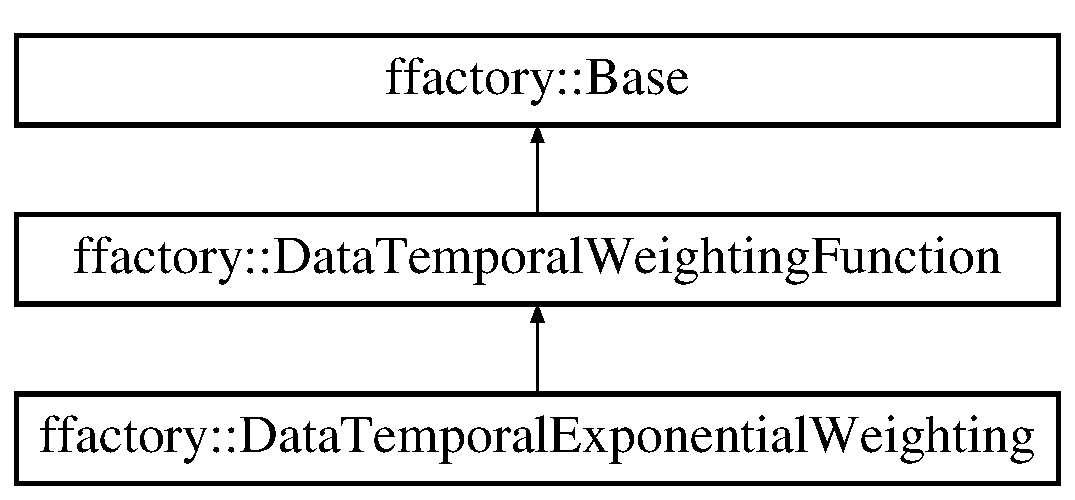
\includegraphics[height=3.000000cm]{classffactory_1_1_data_temporal_exponential_weighting}
\end{center}
\end{figure}
\subsection*{Public Member Functions}
\begin{DoxyCompactItemize}
\item 
\hypertarget{classffactory_1_1_data_temporal_exponential_weighting_a7442853330f60976df9ae1fcdb37b528}{{\bfseries Data\-Temporal\-Exponential\-Weighting} (Data\-Type w)}\label{classffactory_1_1_data_temporal_exponential_weighting_a7442853330f60976df9ae1fcdb37b528}

\item 
virtual Data\-Type \hyperlink{classffactory_1_1_data_temporal_exponential_weighting_a975d766ef91e42aa5e323160749e045e}{set\-Weight} (\hyperlink{classffactory_1_1_sample}{Sample} $\ast$s, Data\-Type t)
\end{DoxyCompactItemize}
\subsection*{Protected Attributes}
\begin{DoxyCompactItemize}
\item 
\hypertarget{classffactory_1_1_data_temporal_exponential_weighting_ae239749dcae99777ae11a07be072937c}{Data\-Type {\bfseries w}}\label{classffactory_1_1_data_temporal_exponential_weighting_ae239749dcae99777ae11a07be072937c}

\end{DoxyCompactItemize}


\subsection{Detailed Description}
Exponential data weighting function $ W(s,t) = e^(wt) $ 

\subsection{Member Function Documentation}
\hypertarget{classffactory_1_1_data_temporal_exponential_weighting_a975d766ef91e42aa5e323160749e045e}{\index{ffactory\-::\-Data\-Temporal\-Exponential\-Weighting@{ffactory\-::\-Data\-Temporal\-Exponential\-Weighting}!set\-Weight@{set\-Weight}}
\index{set\-Weight@{set\-Weight}!ffactory::DataTemporalExponentialWeighting@{ffactory\-::\-Data\-Temporal\-Exponential\-Weighting}}
\subsubsection[{set\-Weight}]{\setlength{\rightskip}{0pt plus 5cm}Data\-Type ffactory\-::\-Data\-Temporal\-Exponential\-Weighting\-::set\-Weight (
\begin{DoxyParamCaption}
\item[{{\bf Sample} $\ast$}]{s, }
\item[{Data\-Type}]{t}
\end{DoxyParamCaption}
)\hspace{0.3cm}{\ttfamily [virtual]}}}\label{classffactory_1_1_data_temporal_exponential_weighting_a975d766ef91e42aa5e323160749e045e}
Method sets weight to \hyperlink{classffactory_1_1_sample}{Sample} object according to time {\itshape t} 
\begin{DoxyParams}{Parameters}
{\em s} & \\
\hline
{\em t} & \\
\hline
\end{DoxyParams}
\begin{DoxyReturn}{Returns}
sample {\itshape s} weight 
\end{DoxyReturn}


Implements \hyperlink{classffactory_1_1_data_temporal_weighting_function_a9388ef364b911239b8cdaa1f24d35f7b}{ffactory\-::\-Data\-Temporal\-Weighting\-Function}.



The documentation for this class was generated from the following files\-:\begin{DoxyCompactItemize}
\item 
src/data/weighting/Data\-Temporal\-Exponential\-Weighting.\-h\item 
src/data/weighting/Data\-Temporal\-Exponential\-Weighting.\-cpp\end{DoxyCompactItemize}

\hypertarget{classffactory_1_1_data_temporal_weighting_function}{\section{ffactory\-:\-:Data\-Temporal\-Weighting\-Function Class Reference}
\label{classffactory_1_1_data_temporal_weighting_function}\index{ffactory\-::\-Data\-Temporal\-Weighting\-Function@{ffactory\-::\-Data\-Temporal\-Weighting\-Function}}
}


{\ttfamily \#include $<$Data\-Temporal\-Weighting\-Function.\-h$>$}

Inheritance diagram for ffactory\-:\-:Data\-Temporal\-Weighting\-Function\-:\begin{figure}[H]
\begin{center}
\leavevmode
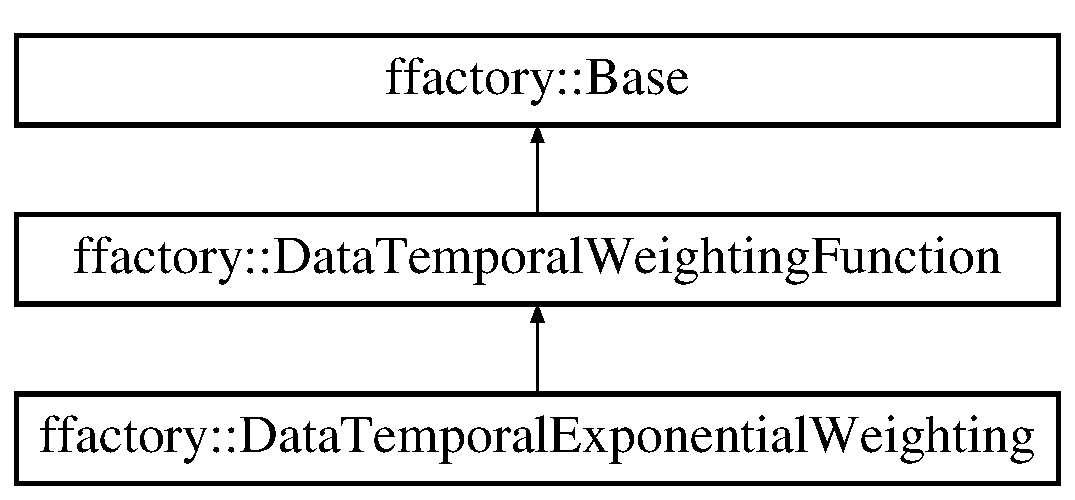
\includegraphics[height=3.000000cm]{classffactory_1_1_data_temporal_weighting_function}
\end{center}
\end{figure}
\subsection*{Public Member Functions}
\begin{DoxyCompactItemize}
\item 
virtual Data\-Type \hyperlink{classffactory_1_1_data_temporal_weighting_function_a9388ef364b911239b8cdaa1f24d35f7b}{set\-Weight} (\hyperlink{classffactory_1_1_sample}{Sample} $\ast$s, Data\-Type t)=0
\end{DoxyCompactItemize}


\subsection{Detailed Description}
Temporal weighting function abstract class 

\subsection{Member Function Documentation}
\hypertarget{classffactory_1_1_data_temporal_weighting_function_a9388ef364b911239b8cdaa1f24d35f7b}{\index{ffactory\-::\-Data\-Temporal\-Weighting\-Function@{ffactory\-::\-Data\-Temporal\-Weighting\-Function}!set\-Weight@{set\-Weight}}
\index{set\-Weight@{set\-Weight}!ffactory::DataTemporalWeightingFunction@{ffactory\-::\-Data\-Temporal\-Weighting\-Function}}
\subsubsection[{set\-Weight}]{\setlength{\rightskip}{0pt plus 5cm}virtual Data\-Type ffactory\-::\-Data\-Temporal\-Weighting\-Function\-::set\-Weight (
\begin{DoxyParamCaption}
\item[{{\bf Sample} $\ast$}]{s, }
\item[{Data\-Type}]{t}
\end{DoxyParamCaption}
)\hspace{0.3cm}{\ttfamily [pure virtual]}}}\label{classffactory_1_1_data_temporal_weighting_function_a9388ef364b911239b8cdaa1f24d35f7b}
Method sets weight to \hyperlink{classffactory_1_1_sample}{Sample} object according to time {\itshape t} 
\begin{DoxyParams}{Parameters}
{\em s} & \\
\hline
{\em t} & \\
\hline
\end{DoxyParams}
\begin{DoxyReturn}{Returns}
sample {\itshape s} weight 
\end{DoxyReturn}


Implemented in \hyperlink{classffactory_1_1_data_temporal_exponential_weighting_a975d766ef91e42aa5e323160749e045e}{ffactory\-::\-Data\-Temporal\-Exponential\-Weighting}.



The documentation for this class was generated from the following file\-:\begin{DoxyCompactItemize}
\item 
src/data/weighting/Data\-Temporal\-Weighting\-Function.\-h\end{DoxyCompactItemize}

\hypertarget{classffactory_1_1_decision_stump}{\section{ffactory\-:\-:Decision\-Stump Class Reference}
\label{classffactory_1_1_decision_stump}\index{ffactory\-::\-Decision\-Stump@{ffactory\-::\-Decision\-Stump}}
}
Inheritance diagram for ffactory\-:\-:Decision\-Stump\-:\begin{figure}[H]
\begin{center}
\leavevmode
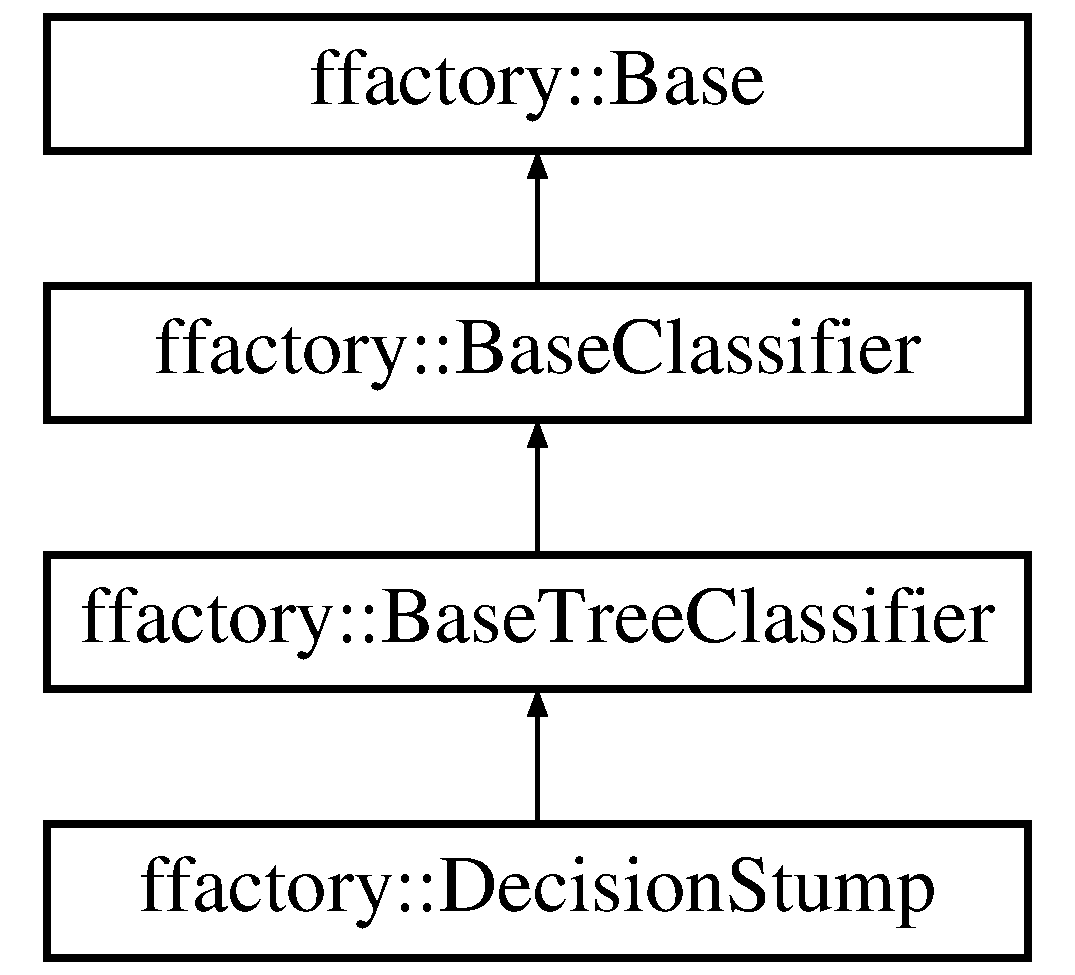
\includegraphics[height=4.000000cm]{classffactory_1_1_decision_stump}
\end{center}
\end{figure}
\subsection*{Public Member Functions}
\begin{DoxyCompactItemize}
\item 
virtual double \hyperlink{classffactory_1_1_decision_stump_ad8ad08ac61f113ca160f01e1e5f9e0f0}{train} (\hyperlink{classffactory_1_1_dataset}{Dataset} d)
\item 
virtual \hyperlink{classffactory_1_1_prediction}{Prediction} \hyperlink{classffactory_1_1_decision_stump_a503571ad46097bec7453e6657c940f2f}{predict} (\hyperlink{classffactory_1_1_sample}{Sample} \&sample)
\item 
virtual std\-::string \hyperlink{classffactory_1_1_decision_stump_af2c5492cfe13d297b11a7aa491695998}{get\-Info} ()
\end{DoxyCompactItemize}
\subsection*{Friends}
\begin{DoxyCompactItemize}
\item 
\hypertarget{classffactory_1_1_decision_stump_abdea50b825108d8d99410d7edc240024}{std\-::ostream \& {\bfseries operator$<$$<$} (std\-::ostream \&stream, \hyperlink{classffactory_1_1_decision_stump}{Decision\-Stump} \&s)}\label{classffactory_1_1_decision_stump_abdea50b825108d8d99410d7edc240024}

\end{DoxyCompactItemize}
\subsection*{Additional Inherited Members}


\subsection{Member Function Documentation}
\hypertarget{classffactory_1_1_decision_stump_af2c5492cfe13d297b11a7aa491695998}{\index{ffactory\-::\-Decision\-Stump@{ffactory\-::\-Decision\-Stump}!get\-Info@{get\-Info}}
\index{get\-Info@{get\-Info}!ffactory::DecisionStump@{ffactory\-::\-Decision\-Stump}}
\subsubsection[{get\-Info}]{\setlength{\rightskip}{0pt plus 5cm}virtual std\-::string ffactory\-::\-Decision\-Stump\-::get\-Info (
\begin{DoxyParamCaption}
{}
\end{DoxyParamCaption}
)\hspace{0.3cm}{\ttfamily [inline]}, {\ttfamily [virtual]}}}\label{classffactory_1_1_decision_stump_af2c5492cfe13d297b11a7aa491695998}
Generates information string \begin{DoxyReturn}{Returns}
std\-::string contains information about classifier 
\end{DoxyReturn}


Reimplemented from \hyperlink{classffactory_1_1_base_classifier_af6b0a89fd34ba70626104500d612d836}{ffactory\-::\-Base\-Classifier}.

\hypertarget{classffactory_1_1_decision_stump_a503571ad46097bec7453e6657c940f2f}{\index{ffactory\-::\-Decision\-Stump@{ffactory\-::\-Decision\-Stump}!predict@{predict}}
\index{predict@{predict}!ffactory::DecisionStump@{ffactory\-::\-Decision\-Stump}}
\subsubsection[{predict}]{\setlength{\rightskip}{0pt plus 5cm}{\bf Prediction} ffactory\-::\-Decision\-Stump\-::predict (
\begin{DoxyParamCaption}
\item[{{\bf Sample} \&}]{sample}
\end{DoxyParamCaption}
)\hspace{0.3cm}{\ttfamily [virtual]}}}\label{classffactory_1_1_decision_stump_a503571ad46097bec7453e6657c940f2f}
Predict class of one sample 
\begin{DoxyParams}{Parameters}
{\em sample} & \\
\hline
\end{DoxyParams}
\begin{DoxyReturn}{Returns}
\hyperlink{classffactory_1_1_prediction}{Prediction} 
\end{DoxyReturn}
\hypertarget{classffactory_1_1_decision_stump_ad8ad08ac61f113ca160f01e1e5f9e0f0}{\index{ffactory\-::\-Decision\-Stump@{ffactory\-::\-Decision\-Stump}!train@{train}}
\index{train@{train}!ffactory::DecisionStump@{ffactory\-::\-Decision\-Stump}}
\subsubsection[{train}]{\setlength{\rightskip}{0pt plus 5cm}double ffactory\-::\-Decision\-Stump\-::train (
\begin{DoxyParamCaption}
\item[{{\bf Dataset}}]{d}
\end{DoxyParamCaption}
)\hspace{0.3cm}{\ttfamily [virtual]}}}\label{classffactory_1_1_decision_stump_ad8ad08ac61f113ca160f01e1e5f9e0f0}
Train classifier on dataset {\itshape d} 
\begin{DoxyParams}{Parameters}
{\em d} & \\
\hline
\end{DoxyParams}
\begin{DoxyReturn}{Returns}
F\-I\-X\-M\-E\-: split\-Score for now. Must be value of specified error measure on dataset {\itshape d} 
\end{DoxyReturn}


The documentation for this class was generated from the following files\-:\begin{DoxyCompactItemize}
\item 
src/classifiers/trees/models/decision\-Stump/decision\-Stump.\-h\item 
src/classifiers/trees/models/decision\-Stump/decision\-Stump.\-cpp\end{DoxyCompactItemize}

\hypertarget{classffactory_1_1_depth_stoppage_criterion}{\section{ffactory\-:\-:Depth\-Stoppage\-Criterion Class Reference}
\label{classffactory_1_1_depth_stoppage_criterion}\index{ffactory\-::\-Depth\-Stoppage\-Criterion@{ffactory\-::\-Depth\-Stoppage\-Criterion}}
}


{\ttfamily \#include $<$depth\-Stoppage\-Criterion.\-h$>$}

Inheritance diagram for ffactory\-:\-:Depth\-Stoppage\-Criterion\-:\begin{figure}[H]
\begin{center}
\leavevmode
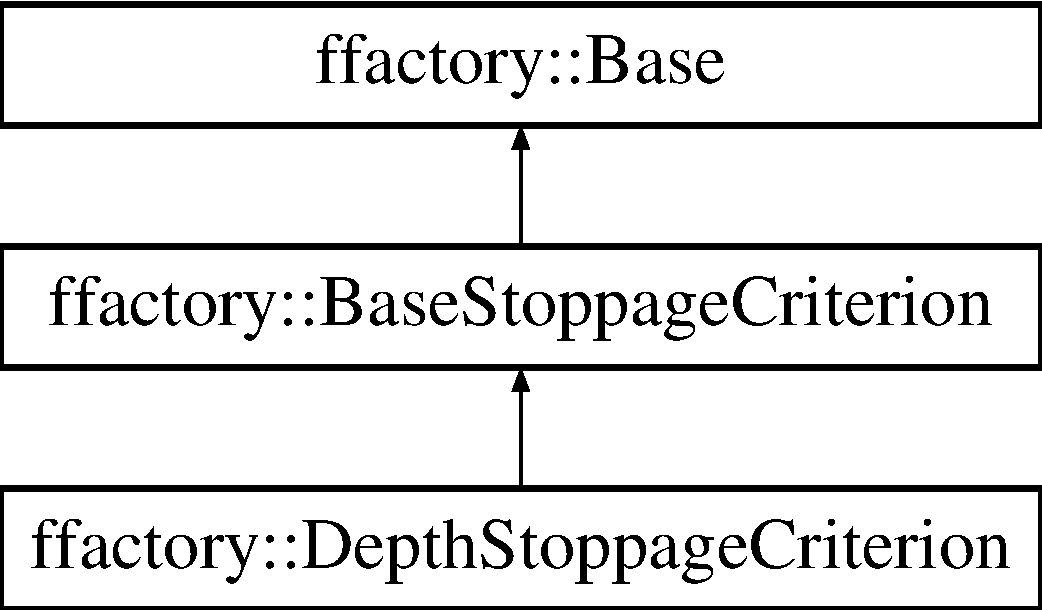
\includegraphics[height=3.000000cm]{classffactory_1_1_depth_stoppage_criterion}
\end{center}
\end{figure}
\subsection*{Public Member Functions}
\begin{DoxyCompactItemize}
\item 
\hypertarget{classffactory_1_1_depth_stoppage_criterion_ad2287a470cebd743f7c7c4226f50885c}{{\bfseries Depth\-Stoppage\-Criterion} (Index\-Type depth)}\label{classffactory_1_1_depth_stoppage_criterion_ad2287a470cebd743f7c7c4226f50885c}

\item 
virtual bool \hyperlink{classffactory_1_1_depth_stoppage_criterion_a363d36a365b10f5d6ad05937c9944ea7}{Is\-Stoppage\-Needed} (\hyperlink{classffactory_1_1_base_tree_node}{Base\-Tree\-Node} $\ast$current\-Node, Data\-Vector \&class\-Prob\-Distr)
\item 
virtual std\-::string \hyperlink{classffactory_1_1_depth_stoppage_criterion_aeb81f88755a7dbae93a176ce8cee5624}{get\-Info} ()
\end{DoxyCompactItemize}


\subsection{Detailed Description}
Stops tree growing on specified depth 

\subsection{Member Function Documentation}
\hypertarget{classffactory_1_1_depth_stoppage_criterion_aeb81f88755a7dbae93a176ce8cee5624}{\index{ffactory\-::\-Depth\-Stoppage\-Criterion@{ffactory\-::\-Depth\-Stoppage\-Criterion}!get\-Info@{get\-Info}}
\index{get\-Info@{get\-Info}!ffactory::DepthStoppageCriterion@{ffactory\-::\-Depth\-Stoppage\-Criterion}}
\subsubsection[{get\-Info}]{\setlength{\rightskip}{0pt plus 5cm}virtual std\-::string ffactory\-::\-Depth\-Stoppage\-Criterion\-::get\-Info (
\begin{DoxyParamCaption}
{}
\end{DoxyParamCaption}
)\hspace{0.3cm}{\ttfamily [inline]}, {\ttfamily [virtual]}}}\label{classffactory_1_1_depth_stoppage_criterion_aeb81f88755a7dbae93a176ce8cee5624}
Generates information string \begin{DoxyReturn}{Returns}
std\-::string contains information about object 
\end{DoxyReturn}


Reimplemented from \hyperlink{classffactory_1_1_base_stoppage_criterion_a0543f9c748cb8092e08314a8d2d40c79}{ffactory\-::\-Base\-Stoppage\-Criterion}.

\hypertarget{classffactory_1_1_depth_stoppage_criterion_a363d36a365b10f5d6ad05937c9944ea7}{\index{ffactory\-::\-Depth\-Stoppage\-Criterion@{ffactory\-::\-Depth\-Stoppage\-Criterion}!Is\-Stoppage\-Needed@{Is\-Stoppage\-Needed}}
\index{Is\-Stoppage\-Needed@{Is\-Stoppage\-Needed}!ffactory::DepthStoppageCriterion@{ffactory\-::\-Depth\-Stoppage\-Criterion}}
\subsubsection[{Is\-Stoppage\-Needed}]{\setlength{\rightskip}{0pt plus 5cm}virtual bool ffactory\-::\-Depth\-Stoppage\-Criterion\-::\-Is\-Stoppage\-Needed (
\begin{DoxyParamCaption}
\item[{{\bf Base\-Tree\-Node} $\ast$}]{current\-Node, }
\item[{Data\-Vector \&}]{class\-Prob\-Distr}
\end{DoxyParamCaption}
)\hspace{0.3cm}{\ttfamily [inline]}, {\ttfamily [virtual]}}}\label{classffactory_1_1_depth_stoppage_criterion_a363d36a365b10f5d6ad05937c9944ea7}
Depth stoppage criterion 
\begin{DoxyParams}{Parameters}
{\em current\-Node} & \\
\hline
{\em class\-Prob\-Distr} & \\
\hline
\end{DoxyParams}
\begin{DoxyReturn}{Returns}

\end{DoxyReturn}


Implements \hyperlink{classffactory_1_1_base_stoppage_criterion_a47728f0c9b241133e228ea5956248241}{ffactory\-::\-Base\-Stoppage\-Criterion}.



The documentation for this class was generated from the following file\-:\begin{DoxyCompactItemize}
\item 
src/classifiers/trees/stoppage\-Criteria/depth\-Stoppage\-Criterion.\-h\end{DoxyCompactItemize}

\hypertarget{classffactory_1_1_empty_stoppage_criterion}{\section{ffactory\-:\-:Empty\-Stoppage\-Criterion Class Reference}
\label{classffactory_1_1_empty_stoppage_criterion}\index{ffactory\-::\-Empty\-Stoppage\-Criterion@{ffactory\-::\-Empty\-Stoppage\-Criterion}}
}


{\ttfamily \#include $<$empty\-Stoppage\-Criterion.\-h$>$}

Inheritance diagram for ffactory\-:\-:Empty\-Stoppage\-Criterion\-:\begin{figure}[H]
\begin{center}
\leavevmode
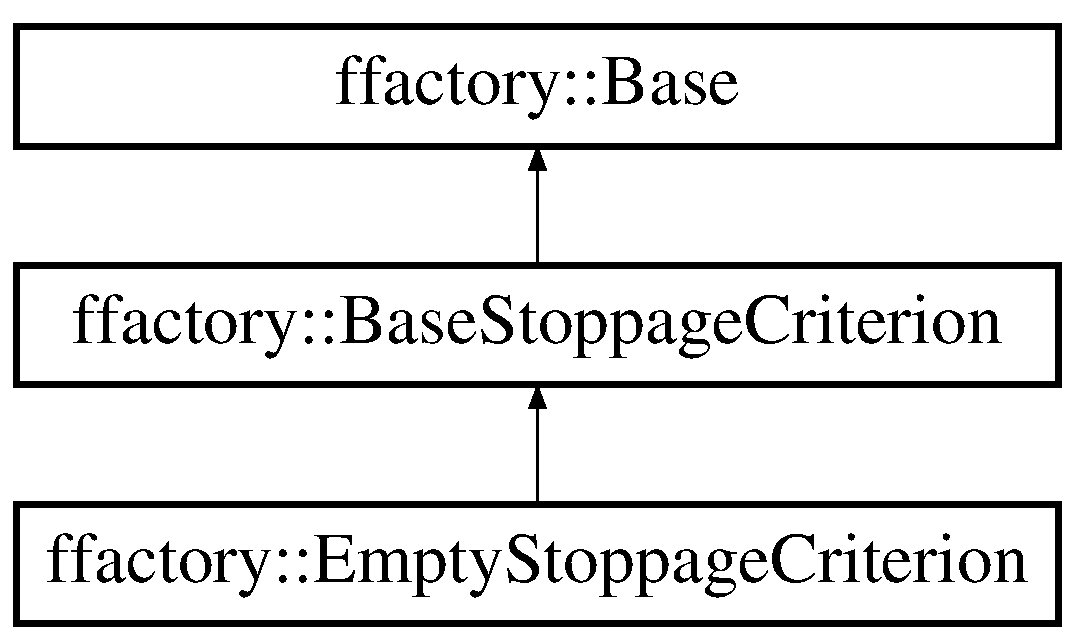
\includegraphics[height=3.000000cm]{classffactory_1_1_empty_stoppage_criterion}
\end{center}
\end{figure}
\subsection*{Public Member Functions}
\begin{DoxyCompactItemize}
\item 
virtual bool \hyperlink{classffactory_1_1_empty_stoppage_criterion_a5dca6353a6a813e09c77b53db8e57fd9}{Is\-Stoppage\-Needed} (\hyperlink{classffactory_1_1_base_tree_node}{Base\-Tree\-Node} $\ast$current\-Node, Data\-Vector \&class\-Prob\-Distr)
\item 
virtual std\-::string \hyperlink{classffactory_1_1_empty_stoppage_criterion_a19181caac08aad7d05fcc07307c93c70}{get\-Info} ()
\end{DoxyCompactItemize}


\subsection{Detailed Description}
Don't stop tree growing at all 

\subsection{Member Function Documentation}
\hypertarget{classffactory_1_1_empty_stoppage_criterion_a19181caac08aad7d05fcc07307c93c70}{\index{ffactory\-::\-Empty\-Stoppage\-Criterion@{ffactory\-::\-Empty\-Stoppage\-Criterion}!get\-Info@{get\-Info}}
\index{get\-Info@{get\-Info}!ffactory::EmptyStoppageCriterion@{ffactory\-::\-Empty\-Stoppage\-Criterion}}
\subsubsection[{get\-Info}]{\setlength{\rightskip}{0pt plus 5cm}virtual std\-::string ffactory\-::\-Empty\-Stoppage\-Criterion\-::get\-Info (
\begin{DoxyParamCaption}
{}
\end{DoxyParamCaption}
)\hspace{0.3cm}{\ttfamily [inline]}, {\ttfamily [virtual]}}}\label{classffactory_1_1_empty_stoppage_criterion_a19181caac08aad7d05fcc07307c93c70}
Generates information string \begin{DoxyReturn}{Returns}
std\-::string contains information about object 
\end{DoxyReturn}


Reimplemented from \hyperlink{classffactory_1_1_base_stoppage_criterion_a0543f9c748cb8092e08314a8d2d40c79}{ffactory\-::\-Base\-Stoppage\-Criterion}.

\hypertarget{classffactory_1_1_empty_stoppage_criterion_a5dca6353a6a813e09c77b53db8e57fd9}{\index{ffactory\-::\-Empty\-Stoppage\-Criterion@{ffactory\-::\-Empty\-Stoppage\-Criterion}!Is\-Stoppage\-Needed@{Is\-Stoppage\-Needed}}
\index{Is\-Stoppage\-Needed@{Is\-Stoppage\-Needed}!ffactory::EmptyStoppageCriterion@{ffactory\-::\-Empty\-Stoppage\-Criterion}}
\subsubsection[{Is\-Stoppage\-Needed}]{\setlength{\rightskip}{0pt plus 5cm}virtual bool ffactory\-::\-Empty\-Stoppage\-Criterion\-::\-Is\-Stoppage\-Needed (
\begin{DoxyParamCaption}
\item[{{\bf Base\-Tree\-Node} $\ast$}]{current\-Node, }
\item[{Data\-Vector \&}]{class\-Prob\-Distr}
\end{DoxyParamCaption}
)\hspace{0.3cm}{\ttfamily [inline]}, {\ttfamily [virtual]}}}\label{classffactory_1_1_empty_stoppage_criterion_a5dca6353a6a813e09c77b53db8e57fd9}
Empty stoppage criterion, it never stops 
\begin{DoxyParams}{Parameters}
{\em current\-Node} & \\
\hline
{\em class\-Prob\-Distr} & \\
\hline
\end{DoxyParams}
\begin{DoxyReturn}{Returns}

\end{DoxyReturn}


Implements \hyperlink{classffactory_1_1_base_stoppage_criterion_a47728f0c9b241133e228ea5956248241}{ffactory\-::\-Base\-Stoppage\-Criterion}.



The documentation for this class was generated from the following file\-:\begin{DoxyCompactItemize}
\item 
src/classifiers/trees/stoppage\-Criteria/empty\-Stoppage\-Criterion.\-h\end{DoxyCompactItemize}

\hypertarget{classffactory_1_1_error_measure_factory}{\section{ffactory\-:\-:Error\-Measure\-Factory Class Reference}
\label{classffactory_1_1_error_measure_factory}\index{ffactory\-::\-Error\-Measure\-Factory@{ffactory\-::\-Error\-Measure\-Factory}}
}
Inheritance diagram for ffactory\-:\-:Error\-Measure\-Factory\-:\begin{figure}[H]
\begin{center}
\leavevmode
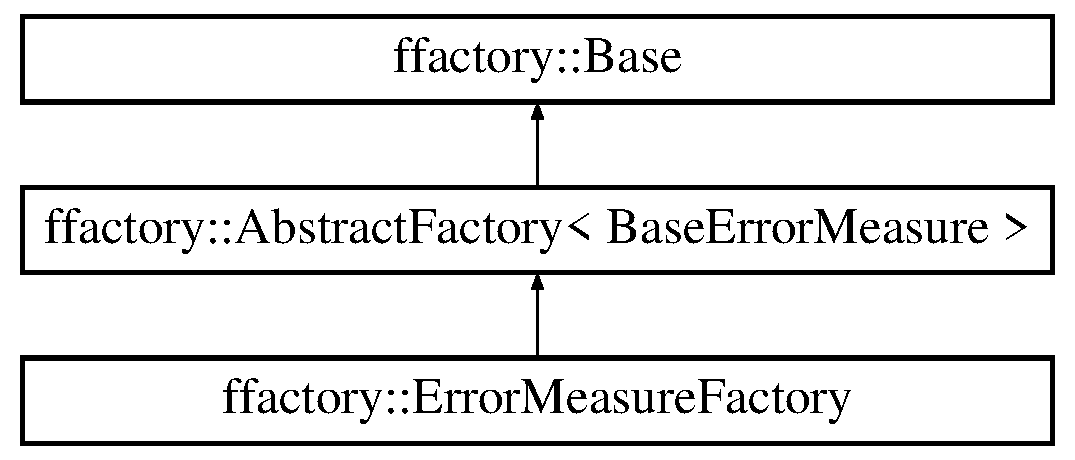
\includegraphics[height=3.000000cm]{classffactory_1_1_error_measure_factory}
\end{center}
\end{figure}
\subsection*{Additional Inherited Members}


The documentation for this class was generated from the following file\-:\begin{DoxyCompactItemize}
\item 
src/classifiers/error\-Measures/Error\-Measure\-Factory.\-h\end{DoxyCompactItemize}

\hypertarget{classffactory_1_1_extremely_randomized_tree}{\section{ffactory\-:\-:Extremely\-Randomized\-Tree Class Reference}
\label{classffactory_1_1_extremely_randomized_tree}\index{ffactory\-::\-Extremely\-Randomized\-Tree@{ffactory\-::\-Extremely\-Randomized\-Tree}}
}


{\ttfamily \#include $<$Extremely\-Randomized\-Tree.\-h$>$}

Inheritance diagram for ffactory\-:\-:Extremely\-Randomized\-Tree\-:\begin{figure}[H]
\begin{center}
\leavevmode
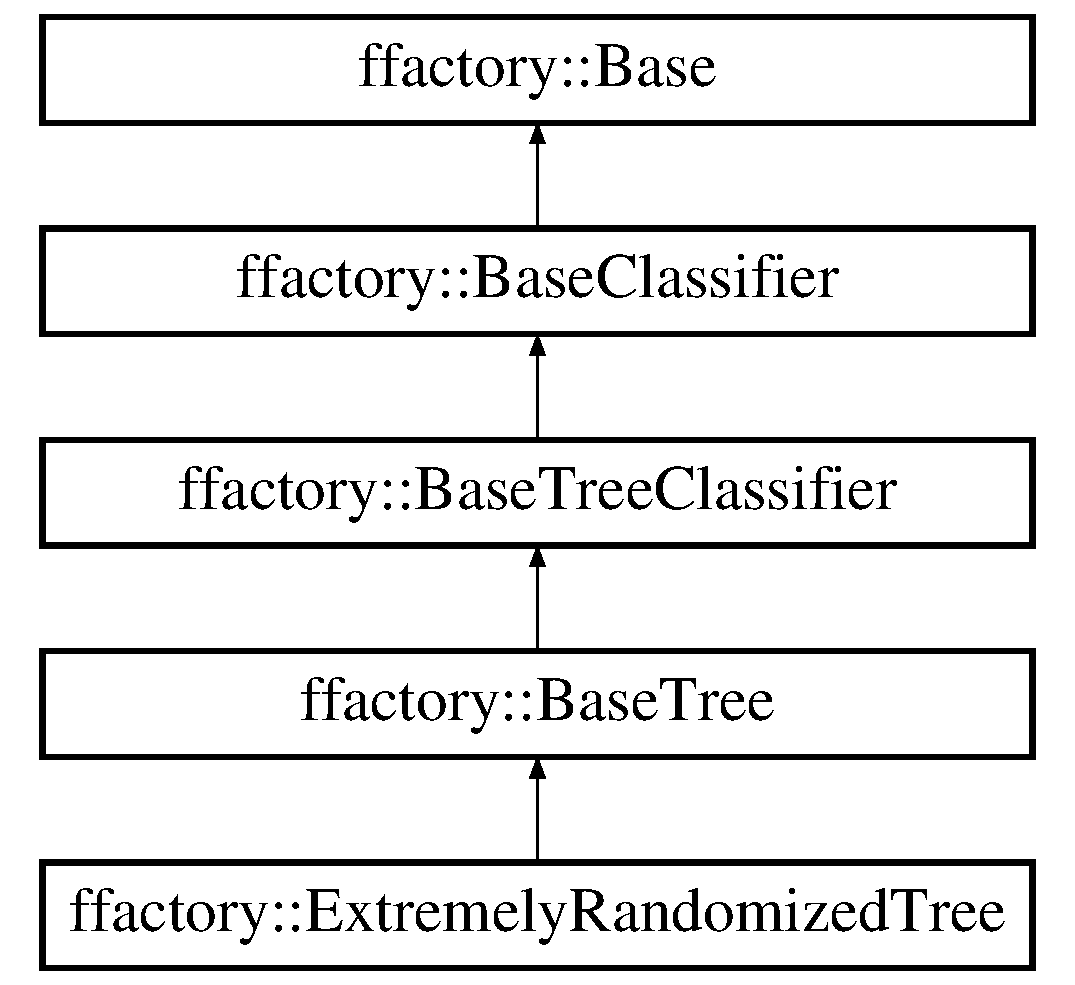
\includegraphics[height=5.000000cm]{classffactory_1_1_extremely_randomized_tree}
\end{center}
\end{figure}
\subsection*{Public Member Functions}
\begin{DoxyCompactItemize}
\item 
\hyperlink{classffactory_1_1_extremely_randomized_tree_a866edb4c45c292babb31c4e25b72fc52}{Extremely\-Randomized\-Tree} ()
\item 
void \hyperlink{classffactory_1_1_extremely_randomized_tree_aefc1d960d78b32160de2b4eb60b99719}{set\-Mtry} (Index\-Type imtry=0)
\end{DoxyCompactItemize}
\subsection*{Additional Inherited Members}


\subsection{Detailed Description}
'Final' implementation of randomized trees as used it original Random Forest 

\subsection{Constructor \& Destructor Documentation}
\hypertarget{classffactory_1_1_extremely_randomized_tree_a866edb4c45c292babb31c4e25b72fc52}{\index{ffactory\-::\-Extremely\-Randomized\-Tree@{ffactory\-::\-Extremely\-Randomized\-Tree}!Extremely\-Randomized\-Tree@{Extremely\-Randomized\-Tree}}
\index{Extremely\-Randomized\-Tree@{Extremely\-Randomized\-Tree}!ffactory::ExtremelyRandomizedTree@{ffactory\-::\-Extremely\-Randomized\-Tree}}
\subsubsection[{Extremely\-Randomized\-Tree}]{\setlength{\rightskip}{0pt plus 5cm}ffactory\-::\-Extremely\-Randomized\-Tree\-::\-Extremely\-Randomized\-Tree (
\begin{DoxyParamCaption}
{}
\end{DoxyParamCaption}
)\hspace{0.3cm}{\ttfamily [inline]}}}\label{classffactory_1_1_extremely_randomized_tree_a866edb4c45c292babb31c4e25b72fc52}
\begin{DoxyRefDesc}{Todo}
\item[\hyperlink{todo__todo000012}{Todo}]set Mtry for classification \end{DoxyRefDesc}


\subsection{Member Function Documentation}
\hypertarget{classffactory_1_1_extremely_randomized_tree_aefc1d960d78b32160de2b4eb60b99719}{\index{ffactory\-::\-Extremely\-Randomized\-Tree@{ffactory\-::\-Extremely\-Randomized\-Tree}!set\-Mtry@{set\-Mtry}}
\index{set\-Mtry@{set\-Mtry}!ffactory::ExtremelyRandomizedTree@{ffactory\-::\-Extremely\-Randomized\-Tree}}
\subsubsection[{set\-Mtry}]{\setlength{\rightskip}{0pt plus 5cm}void ffactory\-::\-Extremely\-Randomized\-Tree\-::set\-Mtry (
\begin{DoxyParamCaption}
\item[{Index\-Type}]{imtry = {\ttfamily 0}}
\end{DoxyParamCaption}
)\hspace{0.3cm}{\ttfamily [inline]}}}\label{classffactory_1_1_extremely_randomized_tree_aefc1d960d78b32160de2b4eb60b99719}
square root from feature number is used by default for classification in classical R\-F 

The documentation for this class was generated from the following file\-:\begin{DoxyCompactItemize}
\item 
src/models/Extremely\-Randomized\-Tree.\-h\end{DoxyCompactItemize}

\hypertarget{classffactory_1_1_extremely_randomized_trees}{\section{ffactory\-:\-:Extremely\-Randomized\-Trees Class Reference}
\label{classffactory_1_1_extremely_randomized_trees}\index{ffactory\-::\-Extremely\-Randomized\-Trees@{ffactory\-::\-Extremely\-Randomized\-Trees}}
}


{\ttfamily \#include $<$Extremely\-Randomized\-Trees.\-h$>$}

Inheritance diagram for ffactory\-:\-:Extremely\-Randomized\-Trees\-:\begin{figure}[H]
\begin{center}
\leavevmode
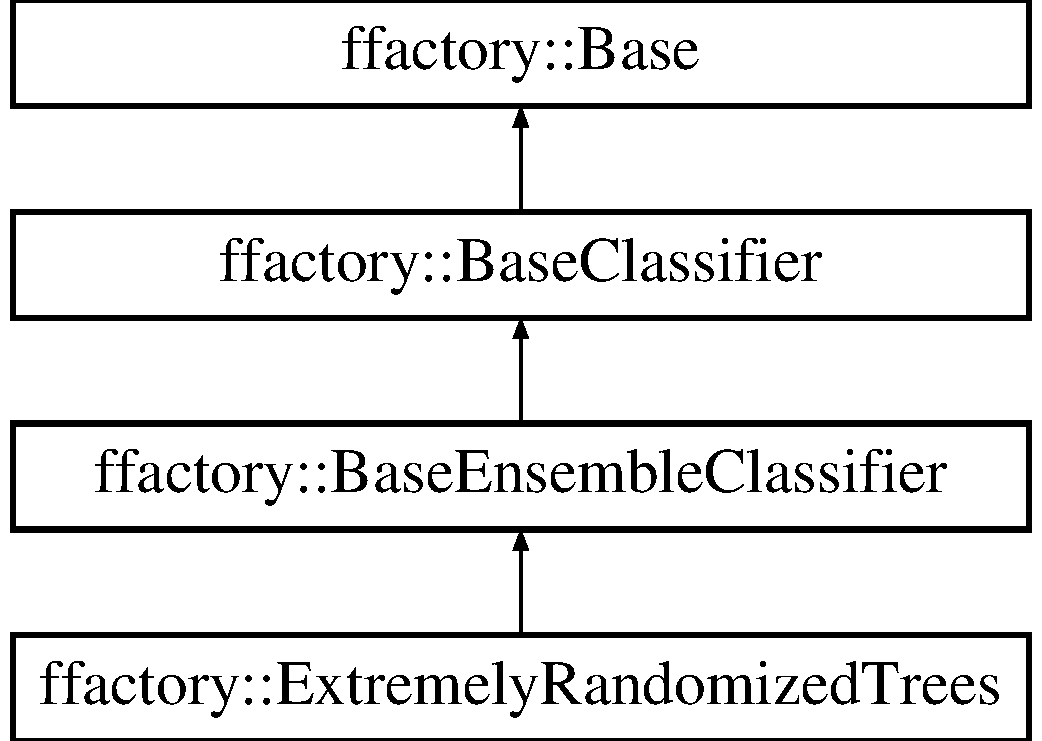
\includegraphics[height=4.000000cm]{classffactory_1_1_extremely_randomized_trees}
\end{center}
\end{figure}
\subsection*{Public Member Functions}
\begin{DoxyCompactItemize}
\item 
\hypertarget{classffactory_1_1_extremely_randomized_trees_aeb67beba0dc4e81389119a50678d62af}{void {\bfseries set\-Num\-Splits} (Index\-Type i)}\label{classffactory_1_1_extremely_randomized_trees_aeb67beba0dc4e81389119a50678d62af}

\item 
\hypertarget{classffactory_1_1_extremely_randomized_trees_af1ec2559f3dafb9d0ea6331b513eb83a}{Index\-Vector $\ast$ {\bfseries get\-Ensemble\-Subset} (Index\-Type cidx)}\label{classffactory_1_1_extremely_randomized_trees_af1ec2559f3dafb9d0ea6331b513eb83a}

\item 
\hypertarget{classffactory_1_1_extremely_randomized_trees_a661844653b70638cda0d00a6c54af495}{{\bfseries Extremely\-Randomized\-Trees} (unsigned int random\-Seed)}\label{classffactory_1_1_extremely_randomized_trees_a661844653b70638cda0d00a6c54af495}

\item 
\hypertarget{classffactory_1_1_extremely_randomized_trees_a9c38d3b661d6bf04aa932101bca8e2c1}{Dataset\-Unique\-Ptr {\bfseries get\-O\-O\-B} (Index\-Type cidx)}\label{classffactory_1_1_extremely_randomized_trees_a9c38d3b661d6bf04aa932101bca8e2c1}

\item 
\hypertarget{classffactory_1_1_extremely_randomized_trees_a752fd75e21b7a64df791a70a7f3816bc}{Data\-Type {\bfseries get\-Classifier\-O\-O\-B\-Error} (Index\-Type cidx)}\label{classffactory_1_1_extremely_randomized_trees_a752fd75e21b7a64df791a70a7f3816bc}

\item 
\hypertarget{classffactory_1_1_extremely_randomized_trees_a4e5d8ebbe450602f0cc34f298c56577c}{Data\-Type {\bfseries get\-O\-O\-B\-Error} ()}\label{classffactory_1_1_extremely_randomized_trees_a4e5d8ebbe450602f0cc34f298c56577c}

\item 
\hypertarget{classffactory_1_1_extremely_randomized_trees_afcdbfab6f57719bfdc4b7e6c8010c37c}{void {\bfseries set\-Mtry\-And\-Splits\-Number} (\hyperlink{classffactory_1_1_base_classifier}{Base\-Classifier} $\ast$bc)}\label{classffactory_1_1_extremely_randomized_trees_afcdbfab6f57719bfdc4b7e6c8010c37c}

\item 
virtual void \hyperlink{classffactory_1_1_extremely_randomized_trees_a31bf52b70e71994cb27814235e3cde43}{train\-New\-Classifier} (\hyperlink{classffactory_1_1_dataset}{Dataset} $\ast$d)
\item 
\hypertarget{classffactory_1_1_extremely_randomized_trees_aa432c99b802b5d2d0d77d39f846e01e6}{void {\bfseries set\-Classifier\-Weight} (Index\-Type cidx, Data\-Type w)}\label{classffactory_1_1_extremely_randomized_trees_aa432c99b802b5d2d0d77d39f846e01e6}

\item 
\hypertarget{classffactory_1_1_extremely_randomized_trees_a7f627dd524d61f4a3c4998fd6108b115}{Data\-Type {\bfseries get\-Classifier\-Weight} (Index\-Type cidx)}\label{classffactory_1_1_extremely_randomized_trees_a7f627dd524d61f4a3c4998fd6108b115}

\item 
\hypertarget{classffactory_1_1_extremely_randomized_trees_a78d678a2ed6f9cc1d8840eb8b7788a99}{void {\bfseries set\-Classifers\-Weights} (Data\-Vector \&mat)}\label{classffactory_1_1_extremely_randomized_trees_a78d678a2ed6f9cc1d8840eb8b7788a99}

\item 
virtual double \hyperlink{classffactory_1_1_extremely_randomized_trees_aa422b510fa91c27fb61eecbd5663cbd8}{train} (\hyperlink{classffactory_1_1_dataset}{Dataset} $\ast$d)
\item 
virtual Data\-Vector\-Unique\-Ptr \hyperlink{classffactory_1_1_extremely_randomized_trees_aed8da96894903e5c8ee7a87add67d78d}{predict\-Class\-Prob} (\hyperlink{classffactory_1_1_sample}{Sample} $\ast$sample)
\item 
\hypertarget{classffactory_1_1_extremely_randomized_trees_aedfa1d3495fa53bedd39ca24d578dd50}{unsigned int {\bfseries get\-Classifiers\-Number} ()}\label{classffactory_1_1_extremely_randomized_trees_aedfa1d3495fa53bedd39ca24d578dd50}

\item 
\hypertarget{classffactory_1_1_extremely_randomized_trees_ae2a706179472df5030c5d882d929f31b}{unsigned int {\bfseries get\-Random\-Seed} () const }\label{classffactory_1_1_extremely_randomized_trees_ae2a706179472df5030c5d882d929f31b}

\item 
\hypertarget{classffactory_1_1_extremely_randomized_trees_a61fdfff8b694983dc66574f307154c77}{void {\bfseries set\-Random\-Seed} (unsigned int random\-Seed)}\label{classffactory_1_1_extremely_randomized_trees_a61fdfff8b694983dc66574f307154c77}

\item 
\hypertarget{classffactory_1_1_extremely_randomized_trees_af12339b80870a7e8cc4426ac8934bc2c}{unsigned int {\bfseries get\-Train\-Subset\-Size} ()}\label{classffactory_1_1_extremely_randomized_trees_af12339b80870a7e8cc4426ac8934bc2c}

\item 
\hypertarget{classffactory_1_1_extremely_randomized_trees_a32c2edfb69796f2c8f319d0e3f734634}{void {\bfseries set\-Train\-Subset\-Size} (unsigned int train\-Subset\-Size)}\label{classffactory_1_1_extremely_randomized_trees_a32c2edfb69796f2c8f319d0e3f734634}

\end{DoxyCompactItemize}
\subsection*{Protected Attributes}
\begin{DoxyCompactItemize}
\item 
\hypertarget{classffactory_1_1_extremely_randomized_trees_a07fda462c8e1bf8bb3679e8e9c1f63bc}{std\-::vector$<$ Index\-Vector $>$ {\bfseries ensemble\-Subsets}}\label{classffactory_1_1_extremely_randomized_trees_a07fda462c8e1bf8bb3679e8e9c1f63bc}

\item 
\hypertarget{classffactory_1_1_extremely_randomized_trees_aea7faf187200de26e153bcd395530a94}{std\-::vector$<$ Data\-Type $>$ {\bfseries ensemble\-Weights}}\label{classffactory_1_1_extremely_randomized_trees_aea7faf187200de26e153bcd395530a94}

\item 
\hypertarget{classffactory_1_1_extremely_randomized_trees_ad308ec46d22a81888bcebad3bb29aea6}{unsigned int {\bfseries random\-Seed}}\label{classffactory_1_1_extremely_randomized_trees_ad308ec46d22a81888bcebad3bb29aea6}

\item 
\hypertarget{classffactory_1_1_extremely_randomized_trees_a5c70d036755477f1ea6694ab0af15b4c}{Index\-Type {\bfseries train\-Subset\-Size}}\label{classffactory_1_1_extremely_randomized_trees_a5c70d036755477f1ea6694ab0af15b4c}

\item 
\hypertarget{classffactory_1_1_extremely_randomized_trees_ab13b780504ea623b9ed02e3f86c9985d}{Randomizer {\bfseries r}}\label{classffactory_1_1_extremely_randomized_trees_ab13b780504ea623b9ed02e3f86c9985d}

\item 
\hypertarget{classffactory_1_1_extremely_randomized_trees_a956c4b7484bcd8646e2302a65e538623}{Index\-Type {\bfseries num\-Splits}}\label{classffactory_1_1_extremely_randomized_trees_a956c4b7484bcd8646e2302a65e538623}

\end{DoxyCompactItemize}


\subsection{Detailed Description}
Weighted Bagging ensemble classifiers for any classifier 

\subsection{Member Function Documentation}
\hypertarget{classffactory_1_1_extremely_randomized_trees_aed8da96894903e5c8ee7a87add67d78d}{\index{ffactory\-::\-Extremely\-Randomized\-Trees@{ffactory\-::\-Extremely\-Randomized\-Trees}!predict\-Class\-Prob@{predict\-Class\-Prob}}
\index{predict\-Class\-Prob@{predict\-Class\-Prob}!ffactory::ExtremelyRandomizedTrees@{ffactory\-::\-Extremely\-Randomized\-Trees}}
\subsubsection[{predict\-Class\-Prob}]{\setlength{\rightskip}{0pt plus 5cm}virtual Data\-Vector\-Unique\-Ptr ffactory\-::\-Extremely\-Randomized\-Trees\-::predict\-Class\-Prob (
\begin{DoxyParamCaption}
\item[{{\bf Sample} $\ast$}]{sample}
\end{DoxyParamCaption}
)\hspace{0.3cm}{\ttfamily [inline]}, {\ttfamily [virtual]}}}\label{classffactory_1_1_extremely_randomized_trees_aed8da96894903e5c8ee7a87add67d78d}
Predict class probability of one sample 
\begin{DoxyParams}{Parameters}
{\em sample} & \\
\hline
\end{DoxyParams}
\begin{DoxyReturn}{Returns}
Index of class 
\end{DoxyReturn}


Implements \hyperlink{classffactory_1_1_base_ensemble_classifier_ac6da7b47a25c7c6481d6476891085d16}{ffactory\-::\-Base\-Ensemble\-Classifier}.

\hypertarget{classffactory_1_1_extremely_randomized_trees_aa422b510fa91c27fb61eecbd5663cbd8}{\index{ffactory\-::\-Extremely\-Randomized\-Trees@{ffactory\-::\-Extremely\-Randomized\-Trees}!train@{train}}
\index{train@{train}!ffactory::ExtremelyRandomizedTrees@{ffactory\-::\-Extremely\-Randomized\-Trees}}
\subsubsection[{train}]{\setlength{\rightskip}{0pt plus 5cm}virtual double ffactory\-::\-Extremely\-Randomized\-Trees\-::train (
\begin{DoxyParamCaption}
\item[{{\bf Dataset} $\ast$}]{d}
\end{DoxyParamCaption}
)\hspace{0.3cm}{\ttfamily [inline]}, {\ttfamily [virtual]}}}\label{classffactory_1_1_extremely_randomized_trees_aa422b510fa91c27fb61eecbd5663cbd8}
Train classifier on dataset {\itshape d} 
\begin{DoxyParams}{Parameters}
{\em d} & \\
\hline
\end{DoxyParams}
\begin{DoxyReturn}{Returns}
Value of specified error measure on dataset {\itshape d} 
\end{DoxyReturn}


Implements \hyperlink{classffactory_1_1_base_ensemble_classifier_a6ea804da2a71766b49372cbddb12cd50}{ffactory\-::\-Base\-Ensemble\-Classifier}.

\hypertarget{classffactory_1_1_extremely_randomized_trees_a31bf52b70e71994cb27814235e3cde43}{\index{ffactory\-::\-Extremely\-Randomized\-Trees@{ffactory\-::\-Extremely\-Randomized\-Trees}!train\-New\-Classifier@{train\-New\-Classifier}}
\index{train\-New\-Classifier@{train\-New\-Classifier}!ffactory::ExtremelyRandomizedTrees@{ffactory\-::\-Extremely\-Randomized\-Trees}}
\subsubsection[{train\-New\-Classifier}]{\setlength{\rightskip}{0pt plus 5cm}virtual void ffactory\-::\-Extremely\-Randomized\-Trees\-::train\-New\-Classifier (
\begin{DoxyParamCaption}
\item[{{\bf Dataset} $\ast$}]{d}
\end{DoxyParamCaption}
)\hspace{0.3cm}{\ttfamily [inline]}, {\ttfamily [virtual]}}}\label{classffactory_1_1_extremely_randomized_trees_a31bf52b70e71994cb27814235e3cde43}
Generate new subset of train dataset and train new classifier on it. Result is pushed to vectors {\itshape ensemble} and {\itshape ensemble\-Subsets} 
\begin{DoxyParams}{Parameters}
{\em d} & \hyperlink{classffactory_1_1_dataset}{Dataset} \\
\hline
\end{DoxyParams}


The documentation for this class was generated from the following file\-:\begin{DoxyCompactItemize}
\item 
src/models/Extremely\-Randomized\-Trees.\-h\end{DoxyCompactItemize}

\hypertarget{classffactory_1_1_factory}{\section{ffactory\-:\-:Factory Class Reference}
\label{classffactory_1_1_factory}\index{ffactory\-::\-Factory@{ffactory\-::\-Factory}}
}
Inheritance diagram for ffactory\-:\-:Factory\-:\begin{figure}[H]
\begin{center}
\leavevmode
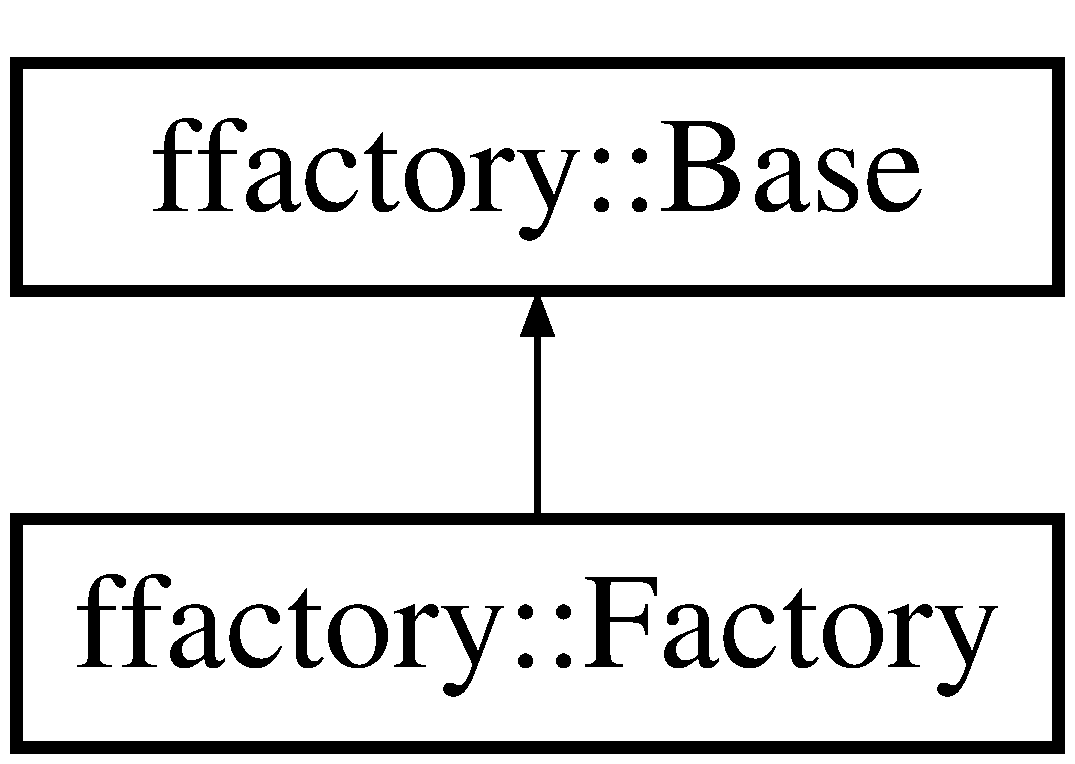
\includegraphics[height=2.000000cm]{classffactory_1_1_factory}
\end{center}
\end{figure}
\subsection*{Public Member Functions}
\begin{DoxyCompactItemize}
\item 
\hypertarget{classffactory_1_1_factory_a9236bfbf74b46f1082696c0d508fbd26}{{\footnotesize template$<$class C $>$ }\\C $\ast$ {\bfseries create} (const std\-::string \&id)}\label{classffactory_1_1_factory_a9236bfbf74b46f1082696c0d508fbd26}

\item 
\hypertarget{classffactory_1_1_factory_adc0f936e2d22ac6327ff62d34032edbc}{{\footnotesize template$<$class C $>$ }\\C $\ast$ {\bfseries create\-Unique} (const std\-::string \&id)}\label{classffactory_1_1_factory_adc0f936e2d22ac6327ff62d34032edbc}

\end{DoxyCompactItemize}


The documentation for this class was generated from the following file\-:\begin{DoxyCompactItemize}
\item 
src/utils/patterns/Abstract\-Factory.\-h\end{DoxyCompactItemize}

\hypertarget{classffactory_1_1_f_f_exception}{\section{ffactory\-:\-:F\-F\-Exception Class Reference}
\label{classffactory_1_1_f_f_exception}\index{ffactory\-::\-F\-F\-Exception@{ffactory\-::\-F\-F\-Exception}}
}


{\ttfamily \#include $<$exceptions.\-h$>$}

Inheritance diagram for ffactory\-:\-:F\-F\-Exception\-:\begin{figure}[H]
\begin{center}
\leavevmode
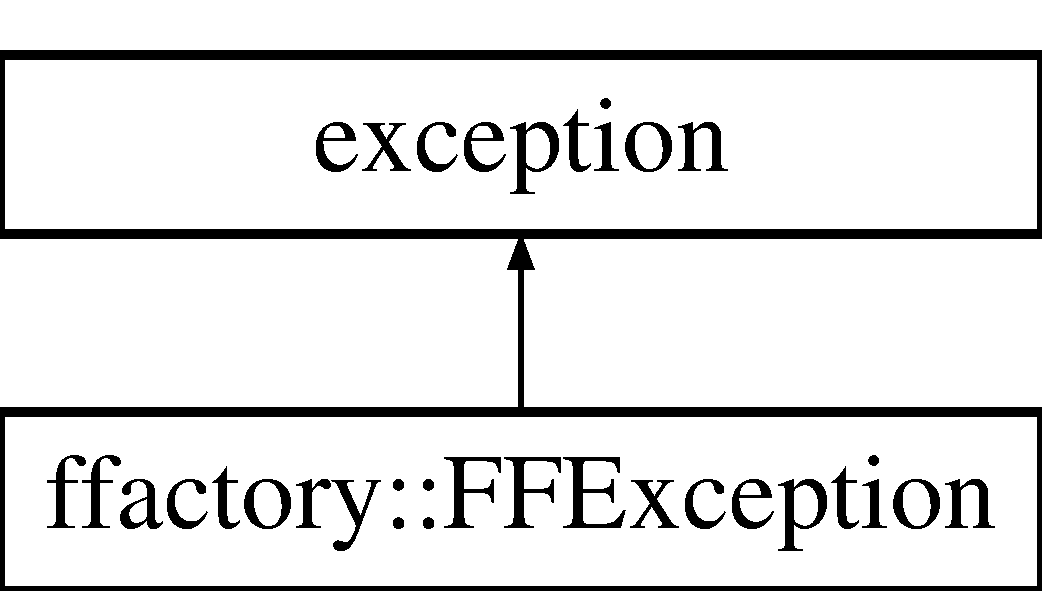
\includegraphics[height=2.000000cm]{classffactory_1_1_f_f_exception}
\end{center}
\end{figure}
\subsection*{Public Member Functions}
\begin{DoxyCompactItemize}
\item 
\hypertarget{classffactory_1_1_f_f_exception_a6cb0d563a738e95ccca6512509f21b7f}{{\bfseries F\-F\-Exception} (\hyperlink{classffactory_1_1_base}{Base} $\ast$object, std\-::string method, std\-::string mes)}\label{classffactory_1_1_f_f_exception_a6cb0d563a738e95ccca6512509f21b7f}

\item 
\hypertarget{classffactory_1_1_f_f_exception_aea73dd281daa06ec098b42e6cf0b8927}{{\bfseries F\-F\-Exception} (std\-::string objectname, std\-::string method, std\-::string mes)}\label{classffactory_1_1_f_f_exception_aea73dd281daa06ec098b42e6cf0b8927}

\item 
\hypertarget{classffactory_1_1_f_f_exception_af4ce78022b1896266b1e9de8784d92f3}{virtual const char $\ast$ {\bfseries what} () const   throw ()}\label{classffactory_1_1_f_f_exception_af4ce78022b1896266b1e9de8784d92f3}

\end{DoxyCompactItemize}


\subsection{Detailed Description}
\hyperlink{classffactory_1_1_base}{Base} exception class 

The documentation for this class was generated from the following file\-:\begin{DoxyCompactItemize}
\item 
src/utils/exceptions.\-h\end{DoxyCompactItemize}

\hypertarget{classffactory_1_1_file_reader_factory}{\section{ffactory\-:\-:File\-Reader\-Factory Class Reference}
\label{classffactory_1_1_file_reader_factory}\index{ffactory\-::\-File\-Reader\-Factory@{ffactory\-::\-File\-Reader\-Factory}}
}


{\ttfamily \#include $<$File\-Reader\-Factory.\-h$>$}

Inheritance diagram for ffactory\-:\-:File\-Reader\-Factory\-:\begin{figure}[H]
\begin{center}
\leavevmode
\includegraphics[height=3.000000cm]{classffactory_1_1_file_reader_factory}
\end{center}
\end{figure}
\subsection*{Public Member Functions}
\begin{DoxyCompactItemize}
\item 
virtual void \hyperlink{classffactory_1_1_file_reader_factory_a0f0b807dc1c92452b1cb97187ddf9f33}{Register} ()
\item 
\hypertarget{classffactory_1_1_file_reader_factory_a7674c4a7bde811450a391792eecc8ff4}{virtual void {\bfseries read} (const char $\ast$file, const char $\ast$format, \hyperlink{classffactory_1_1_dataset}{Dataset} $\ast$d)}\label{classffactory_1_1_file_reader_factory_a7674c4a7bde811450a391792eecc8ff4}

\end{DoxyCompactItemize}


\subsection{Detailed Description}
Class is used to read files of different formats 

\subsection{Member Function Documentation}
\hypertarget{classffactory_1_1_file_reader_factory_a0f0b807dc1c92452b1cb97187ddf9f33}{\index{ffactory\-::\-File\-Reader\-Factory@{ffactory\-::\-File\-Reader\-Factory}!Register@{Register}}
\index{Register@{Register}!ffactory::FileReaderFactory@{ffactory\-::\-File\-Reader\-Factory}}
\subsubsection[{Register}]{\setlength{\rightskip}{0pt plus 5cm}virtual void ffactory\-::\-File\-Reader\-Factory\-::\-Register (
\begin{DoxyParamCaption}
{}
\end{DoxyParamCaption}
)\hspace{0.3cm}{\ttfamily [inline]}, {\ttfamily [virtual]}}}\label{classffactory_1_1_file_reader_factory_a0f0b807dc1c92452b1cb97187ddf9f33}
Function must be called before using the class 

Implements \hyperlink{classffactory_1_1_abstract_factory_acc3b114aecc19f8b4de596dba5bc7786}{ffactory\-::\-Abstract\-Factory$<$ Base\-File\-Reader $>$}.



The documentation for this class was generated from the following file\-:\begin{DoxyCompactItemize}
\item 
src/data/file\-Formats/File\-Reader\-Factory.\-h\end{DoxyCompactItemize}

\hypertarget{classffactory_1_1_file_writer_factory}{\section{ffactory\-:\-:File\-Writer\-Factory Class Reference}
\label{classffactory_1_1_file_writer_factory}\index{ffactory\-::\-File\-Writer\-Factory@{ffactory\-::\-File\-Writer\-Factory}}
}


{\ttfamily \#include $<$File\-Writer\-Factory.\-h$>$}

Inheritance diagram for ffactory\-:\-:File\-Writer\-Factory\-:\begin{figure}[H]
\begin{center}
\leavevmode
\includegraphics[height=3.000000cm]{classffactory_1_1_file_writer_factory}
\end{center}
\end{figure}
\subsection*{Additional Inherited Members}


\subsection{Detailed Description}
Class is used to read files of different formats 

The documentation for this class was generated from the following file\-:\begin{DoxyCompactItemize}
\item 
src/data/file\-Formats/File\-Writer\-Factory.\-h\end{DoxyCompactItemize}

\hypertarget{classffactory_1_1_gini_impurity_measure}{\section{ffactory\-:\-:Gini\-Impurity\-Measure Class Reference}
\label{classffactory_1_1_gini_impurity_measure}\index{ffactory\-::\-Gini\-Impurity\-Measure@{ffactory\-::\-Gini\-Impurity\-Measure}}
}
Inheritance diagram for ffactory\-:\-:Gini\-Impurity\-Measure\-:\begin{figure}[H]
\begin{center}
\leavevmode
\includegraphics[height=3.000000cm]{classffactory_1_1_gini_impurity_measure}
\end{center}
\end{figure}
\subsection*{Public Member Functions}
\begin{DoxyCompactItemize}
\item 
virtual double \hyperlink{classffactory_1_1_gini_impurity_measure_afad0349dd370af15c9b3334cd33e9a70}{calculate} (double p)
\end{DoxyCompactItemize}


\subsection{Member Function Documentation}
\hypertarget{classffactory_1_1_gini_impurity_measure_afad0349dd370af15c9b3334cd33e9a70}{\index{ffactory\-::\-Gini\-Impurity\-Measure@{ffactory\-::\-Gini\-Impurity\-Measure}!calculate@{calculate}}
\index{calculate@{calculate}!ffactory::GiniImpurityMeasure@{ffactory\-::\-Gini\-Impurity\-Measure}}
\subsubsection[{calculate}]{\setlength{\rightskip}{0pt plus 5cm}virtual double ffactory\-::\-Gini\-Impurity\-Measure\-::calculate (
\begin{DoxyParamCaption}
\item[{double}]{p}
\end{DoxyParamCaption}
)\hspace{0.3cm}{\ttfamily [inline]}, {\ttfamily [virtual]}}}\label{classffactory_1_1_gini_impurity_measure_afad0349dd370af15c9b3334cd33e9a70}
Gini-\/index used as Impurity measure function 
\begin{DoxyParams}{Parameters}
{\em p} & \\
\hline
\end{DoxyParams}
\begin{DoxyReturn}{Returns}
impurity score 
\end{DoxyReturn}


Implements \hyperlink{classffactory_1_1_base_impurity_measure_ad0e0127a42c1ece9658ebf07e2b26efe}{ffactory\-::\-Base\-Impurity\-Measure}.



The documentation for this class was generated from the following file\-:\begin{DoxyCompactItemize}
\item 
src/classifiers/trees/impurity\-Measures/gini\-Impurity\-Measure.\-h\end{DoxyCompactItemize}

\hypertarget{classffactory_1_1_impurity_measure_factory}{\section{ffactory\-:\-:Impurity\-Measure\-Factory Class Reference}
\label{classffactory_1_1_impurity_measure_factory}\index{ffactory\-::\-Impurity\-Measure\-Factory@{ffactory\-::\-Impurity\-Measure\-Factory}}
}
Inheritance diagram for ffactory\-:\-:Impurity\-Measure\-Factory\-:\begin{figure}[H]
\begin{center}
\leavevmode
\includegraphics[height=3.000000cm]{classffactory_1_1_impurity_measure_factory}
\end{center}
\end{figure}
\subsection*{Additional Inherited Members}


The documentation for this class was generated from the following file\-:\begin{DoxyCompactItemize}
\item 
src/classifiers/trees/impurity\-Measures/Impurity\-Measure\-Factory.\-h\end{DoxyCompactItemize}

\hypertarget{classffactory_1_1_info_gain_impurity_measure}{\section{ffactory\-:\-:Info\-Gain\-Impurity\-Measure Class Reference}
\label{classffactory_1_1_info_gain_impurity_measure}\index{ffactory\-::\-Info\-Gain\-Impurity\-Measure@{ffactory\-::\-Info\-Gain\-Impurity\-Measure}}
}
Inheritance diagram for ffactory\-:\-:Info\-Gain\-Impurity\-Measure\-:\begin{figure}[H]
\begin{center}
\leavevmode
\includegraphics[height=3.000000cm]{classffactory_1_1_info_gain_impurity_measure}
\end{center}
\end{figure}
\subsection*{Public Member Functions}
\begin{DoxyCompactItemize}
\item 
virtual double \hyperlink{classffactory_1_1_info_gain_impurity_measure_a1996955c9df6847f0fccdd36112655b3}{calculate} (double p)
\end{DoxyCompactItemize}


\subsection{Member Function Documentation}
\hypertarget{classffactory_1_1_info_gain_impurity_measure_a1996955c9df6847f0fccdd36112655b3}{\index{ffactory\-::\-Info\-Gain\-Impurity\-Measure@{ffactory\-::\-Info\-Gain\-Impurity\-Measure}!calculate@{calculate}}
\index{calculate@{calculate}!ffactory::InfoGainImpurityMeasure@{ffactory\-::\-Info\-Gain\-Impurity\-Measure}}
\subsubsection[{calculate}]{\setlength{\rightskip}{0pt plus 5cm}virtual double ffactory\-::\-Info\-Gain\-Impurity\-Measure\-::calculate (
\begin{DoxyParamCaption}
\item[{double}]{p}
\end{DoxyParamCaption}
)\hspace{0.3cm}{\ttfamily [inline]}, {\ttfamily [virtual]}}}\label{classffactory_1_1_info_gain_impurity_measure_a1996955c9df6847f0fccdd36112655b3}
Information gain used as Impurity measure function 
\begin{DoxyParams}{Parameters}
{\em p} & \\
\hline
\end{DoxyParams}
\begin{DoxyReturn}{Returns}
impurity score 
\end{DoxyReturn}


Implements \hyperlink{classffactory_1_1_base_impurity_measure_ad0e0127a42c1ece9658ebf07e2b26efe}{ffactory\-::\-Base\-Impurity\-Measure}.



The documentation for this class was generated from the following file\-:\begin{DoxyCompactItemize}
\item 
src/classifiers/trees/impurity\-Measures/info\-Gain\-Impurity\-Measure.\-h\end{DoxyCompactItemize}

\hypertarget{classffactory_1_1_missclassification_error_measure}{\section{ffactory\-:\-:Missclassification\-Error\-Measure Class Reference}
\label{classffactory_1_1_missclassification_error_measure}\index{ffactory\-::\-Missclassification\-Error\-Measure@{ffactory\-::\-Missclassification\-Error\-Measure}}
}


{\ttfamily \#include $<$Missclassification\-Error\-Measure.\-h$>$}

Inheritance diagram for ffactory\-:\-:Missclassification\-Error\-Measure\-:\begin{figure}[H]
\begin{center}
\leavevmode
\includegraphics[height=3.000000cm]{classffactory_1_1_missclassification_error_measure}
\end{center}
\end{figure}
\subsection*{Public Member Functions}
\begin{DoxyCompactItemize}
\item 
virtual double \hyperlink{classffactory_1_1_missclassification_error_measure_adedf3d4ccccf1dd24995d9e5d109afd3}{get\-Error} (\hyperlink{classffactory_1_1_base_classifier}{Base\-Classifier} $\ast$c, \hyperlink{classffactory_1_1_sample}{Sample} \&s)
\item 
virtual double \hyperlink{classffactory_1_1_missclassification_error_measure_a962d88274011caaba227e7c7f6ce3bdf}{get\-Error} (\hyperlink{classffactory_1_1_base_classifier}{Base\-Classifier} $\ast$c, \hyperlink{classffactory_1_1_dataset}{Dataset} $\ast$d)
\end{DoxyCompactItemize}


\subsection{Detailed Description}
Missclassification error measure class 

\subsection{Member Function Documentation}
\hypertarget{classffactory_1_1_missclassification_error_measure_adedf3d4ccccf1dd24995d9e5d109afd3}{\index{ffactory\-::\-Missclassification\-Error\-Measure@{ffactory\-::\-Missclassification\-Error\-Measure}!get\-Error@{get\-Error}}
\index{get\-Error@{get\-Error}!ffactory::MissclassificationErrorMeasure@{ffactory\-::\-Missclassification\-Error\-Measure}}
\subsubsection[{get\-Error}]{\setlength{\rightskip}{0pt plus 5cm}virtual double ffactory\-::\-Missclassification\-Error\-Measure\-::get\-Error (
\begin{DoxyParamCaption}
\item[{{\bf Base\-Classifier} $\ast$}]{c, }
\item[{{\bf Sample} \&}]{s}
\end{DoxyParamCaption}
)\hspace{0.3cm}{\ttfamily [inline]}, {\ttfamily [virtual]}}}\label{classffactory_1_1_missclassification_error_measure_adedf3d4ccccf1dd24995d9e5d109afd3}
Get error on current sample {\itshape s} 
\begin{DoxyParams}{Parameters}
{\em s} & \\
\hline
\end{DoxyParams}
\begin{DoxyReturn}{Returns}
probability of wrong classes 
\end{DoxyReturn}


Implements \hyperlink{classffactory_1_1_base_error_measure_a8eb4fef1cb479834c3fc1baac589d8b1}{ffactory\-::\-Base\-Error\-Measure}.

\hypertarget{classffactory_1_1_missclassification_error_measure_a962d88274011caaba227e7c7f6ce3bdf}{\index{ffactory\-::\-Missclassification\-Error\-Measure@{ffactory\-::\-Missclassification\-Error\-Measure}!get\-Error@{get\-Error}}
\index{get\-Error@{get\-Error}!ffactory::MissclassificationErrorMeasure@{ffactory\-::\-Missclassification\-Error\-Measure}}
\subsubsection[{get\-Error}]{\setlength{\rightskip}{0pt plus 5cm}virtual double ffactory\-::\-Missclassification\-Error\-Measure\-::get\-Error (
\begin{DoxyParamCaption}
\item[{{\bf Base\-Classifier} $\ast$}]{c, }
\item[{{\bf Dataset} $\ast$}]{d}
\end{DoxyParamCaption}
)\hspace{0.3cm}{\ttfamily [inline]}, {\ttfamily [virtual]}}}\label{classffactory_1_1_missclassification_error_measure_a962d88274011caaba227e7c7f6ce3bdf}
Get error on entire dataset {\itshape d} 
\begin{DoxyParams}{Parameters}
{\em d} & \\
\hline
\end{DoxyParams}
\begin{DoxyReturn}{Returns}
average 
\end{DoxyReturn}


Implements \hyperlink{classffactory_1_1_base_error_measure_a59333613908d58b1a5ff7208bd93d6fb}{ffactory\-::\-Base\-Error\-Measure}.



The documentation for this class was generated from the following file\-:\begin{DoxyCompactItemize}
\item 
src/classifiers/error\-Measures/Missclassification\-Error\-Measure.\-h\end{DoxyCompactItemize}

\hypertarget{classffactory_1_1_online_random_forest}{\section{ffactory\-:\-:Online\-Random\-Forest Class Reference}
\label{classffactory_1_1_online_random_forest}\index{ffactory\-::\-Online\-Random\-Forest@{ffactory\-::\-Online\-Random\-Forest}}
}
Inheritance diagram for ffactory\-:\-:Online\-Random\-Forest\-:\begin{figure}[H]
\begin{center}
\leavevmode
\includegraphics[height=3.000000cm]{classffactory_1_1_online_random_forest}
\end{center}
\end{figure}
\subsection*{Public Member Functions}
\begin{DoxyCompactItemize}
\item 
virtual double \hyperlink{classffactory_1_1_online_random_forest_af0c36073053407883c7ddd1fce631d7f}{update} (\hyperlink{classffactory_1_1_dataset}{Dataset} $\ast$newdata)
\end{DoxyCompactItemize}


\subsection{Member Function Documentation}
\hypertarget{classffactory_1_1_online_random_forest_af0c36073053407883c7ddd1fce631d7f}{\index{ffactory\-::\-Online\-Random\-Forest@{ffactory\-::\-Online\-Random\-Forest}!update@{update}}
\index{update@{update}!ffactory::OnlineRandomForest@{ffactory\-::\-Online\-Random\-Forest}}
\subsubsection[{update}]{\setlength{\rightskip}{0pt plus 5cm}virtual double ffactory\-::\-Online\-Random\-Forest\-::update (
\begin{DoxyParamCaption}
\item[{{\bf Dataset} $\ast$}]{newdata}
\end{DoxyParamCaption}
)\hspace{0.3cm}{\ttfamily [inline]}, {\ttfamily [virtual]}}}\label{classffactory_1_1_online_random_forest_af0c36073053407883c7ddd1fce631d7f}
Main class for update model with {\itshape newdata} 

Reimplemented from \hyperlink{classffactory_1_1_base_online_classifier_a1f4c58973708b188e99651ed0b82631d}{ffactory\-::\-Base\-Online\-Classifier}.



The documentation for this class was generated from the following files\-:\begin{DoxyCompactItemize}
\item 
src/models/Online\-Random\-Forest.\-h\item 
src/models/Online\-Random\-Forest.\-cpp\end{DoxyCompactItemize}

\hypertarget{classffactory_1_1_parameter_set}{\section{ffactory\-:\-:Parameter\-Set Class Reference}
\label{classffactory_1_1_parameter_set}\index{ffactory\-::\-Parameter\-Set@{ffactory\-::\-Parameter\-Set}}
}
\subsection*{Public Member Functions}
\begin{DoxyCompactItemize}
\item 
\hypertarget{classffactory_1_1_parameter_set_a189575862c8e4bdc222d64d9dc5ce241}{uint32\-\_\-t {\bfseries get\-Value\-Number} ()}\label{classffactory_1_1_parameter_set_a189575862c8e4bdc222d64d9dc5ce241}

\item 
\hypertarget{classffactory_1_1_parameter_set_a833575fbee435803d92e3eacf72fb06b}{double {\bfseries get\-Current\-Value} ()}\label{classffactory_1_1_parameter_set_a833575fbee435803d92e3eacf72fb06b}

\item 
\hypertarget{classffactory_1_1_parameter_set_a6f3a2b7a04890c2e803b7d7162af0e2e}{void {\bfseries set\-Current\-Index} (uint32\-\_\-t current\-Index)}\label{classffactory_1_1_parameter_set_a6f3a2b7a04890c2e803b7d7162af0e2e}

\item 
\hypertarget{classffactory_1_1_parameter_set_a1b7addd8235b6b3ee2536e8803972f49}{const std\-::string \& {\bfseries get\-Name} () const }\label{classffactory_1_1_parameter_set_a1b7addd8235b6b3ee2536e8803972f49}

\item 
\hypertarget{classffactory_1_1_parameter_set_a0ae54904ef6a4fedb3556bb511c600d1}{void {\bfseries set\-Name} (const std\-::string \&name)}\label{classffactory_1_1_parameter_set_a0ae54904ef6a4fedb3556bb511c600d1}

\item 
\hypertarget{classffactory_1_1_parameter_set_abf99a69dd39a0d5a40529be5f5920ffe}{std\-::vector$<$ double $>$ $\ast$ {\bfseries get\-Values} ()}\label{classffactory_1_1_parameter_set_abf99a69dd39a0d5a40529be5f5920ffe}

\item 
\hypertarget{classffactory_1_1_parameter_set_a8e13fb085b13835ef37a03570d337925}{void {\bfseries set\-Values} (std\-::vector$<$ double $>$ \&values)}\label{classffactory_1_1_parameter_set_a8e13fb085b13835ef37a03570d337925}

\item 
\hypertarget{classffactory_1_1_parameter_set_a38977f735d79efdaa74cb6299423485c}{void {\bfseries add\-Value} (double value)}\label{classffactory_1_1_parameter_set_a38977f735d79efdaa74cb6299423485c}

\item 
\hypertarget{classffactory_1_1_parameter_set_a41cb3c22a42d40a80312bf0f8c3361c6}{double {\bfseries get\-Value} (uint32\-\_\-t index)}\label{classffactory_1_1_parameter_set_a41cb3c22a42d40a80312bf0f8c3361c6}

\end{DoxyCompactItemize}


The documentation for this class was generated from the following file\-:\begin{DoxyCompactItemize}
\item 
src/testers/Base\-Classifier\-Tester.\-h\end{DoxyCompactItemize}

\hypertarget{classffactory_1_1_partition_statistics}{\section{ffactory\-:\-:Partition\-Statistics Class Reference}
\label{classffactory_1_1_partition_statistics}\index{ffactory\-::\-Partition\-Statistics@{ffactory\-::\-Partition\-Statistics}}
}


{\ttfamily \#include $<$Partition\-Statistics.\-h$>$}

\subsection*{Public Member Functions}
\begin{DoxyCompactItemize}
\item 
\hypertarget{classffactory_1_1_partition_statistics_afc85cfef9d4853d5ea8995329daa641e}{void {\bfseries copy\-Statistics} (\hyperlink{classffactory_1_1_partition_statistics}{Partition\-Statistics} \&stat)}\label{classffactory_1_1_partition_statistics_afc85cfef9d4853d5ea8995329daa641e}

\item 
\hypertarget{classffactory_1_1_partition_statistics_a0a7ab8fec6d7825f3fd1c86c110b8cb1}{\hyperlink{classffactory_1_1_partition_statistics}{Partition\-Statistics} \& {\bfseries operator=} (\hyperlink{classffactory_1_1_partition_statistics}{Partition\-Statistics} \&other)}\label{classffactory_1_1_partition_statistics_a0a7ab8fec6d7825f3fd1c86c110b8cb1}

\item 
\hypertarget{classffactory_1_1_partition_statistics_ac51554ea5f08d0277dd69d6878b7a928}{{\bfseries Partition\-Statistics} (\hyperlink{classffactory_1_1_partition_statistics}{Partition\-Statistics} \&other)}\label{classffactory_1_1_partition_statistics_ac51554ea5f08d0277dd69d6878b7a928}

\item 
\hypertarget{classffactory_1_1_partition_statistics_a7180a6a215b82b62f836994fe5a0832c}{{\bfseries Partition\-Statistics} (Index\-Type num\-Classes, Index\-Type num\-Features, std\-::vector$<$ \hyperlink{classffactory_1_1_sample}{Sample} $>$ $\ast$data=N\-U\-L\-L, \hyperlink{classffactory_1_1_data_ranges}{Data\-Ranges} $\ast$dr=N\-U\-L\-L, \hyperlink{classffactory_1_1_data_ranges}{Data\-Ranges} $\ast$global\-Ranges=N\-U\-L\-L)}\label{classffactory_1_1_partition_statistics_a7180a6a215b82b62f836994fe5a0832c}

\item 
\hypertarget{classffactory_1_1_partition_statistics_a30876f6676c6aee2060f5657261df141}{void {\bfseries add\-Samples} (std\-::vector$<$ \hyperlink{classffactory_1_1_sample}{Sample} $>$ $\ast$data)}\label{classffactory_1_1_partition_statistics_a30876f6676c6aee2060f5657261df141}

\item 
\hypertarget{classffactory_1_1_partition_statistics_a7b57d257f59718ede48cf21e94da8b8f}{void {\bfseries add\-Samples\-In\-Range} (std\-::vector$<$ \hyperlink{classffactory_1_1_sample}{Sample} $>$ $\ast$data)}\label{classffactory_1_1_partition_statistics_a7b57d257f59718ede48cf21e94da8b8f}

\item 
virtual \hyperlink{classffactory_1_1_partition_statistics_a4c838e480cc0fb6c9ac93e9abf0e9613}{$\sim$\-Partition\-Statistics} ()
\item 
\hypertarget{classffactory_1_1_partition_statistics_a6e953b946f5a7fd73210524c4e76a2a7}{void {\bfseries add\-Categorial\-Partition\-Ranges} (Index\-Type attr\-Idx, Data\-Type category)}\label{classffactory_1_1_partition_statistics_a6e953b946f5a7fd73210524c4e76a2a7}

\item 
void \hyperlink{classffactory_1_1_partition_statistics_a991b8a7b65034632781fb1650654e7d0}{remove\-Sample} (\hyperlink{classffactory_1_1_sample}{Sample} $\ast$const s)
\item 
void \hyperlink{classffactory_1_1_partition_statistics_a340f7b5f795fcdbe2d448ccfce86a32e}{add\-Point} (\hyperlink{classffactory_1_1_sample}{Sample} $\ast$const s)
\item 
void \hyperlink{classffactory_1_1_partition_statistics_a1acdc107481f49362175355b8530e32c}{add\-Point\-In\-Range} (\hyperlink{classffactory_1_1_sample}{Sample} $\ast$const s)
\item 
void \hyperlink{classffactory_1_1_partition_statistics_afe3bee838f0967a7840573eafb9194d8}{init\-Data\-Ranges} (\hyperlink{classffactory_1_1_data_ranges}{Data\-Ranges} $\ast$dr=N\-U\-L\-L)
\item 
void \hyperlink{classffactory_1_1_partition_statistics_a73651a96a6221a45e850876241563ee6}{init\-Sample\-Statistics} (std\-::vector$<$ \hyperlink{classffactory_1_1_sample}{Sample} $>$ $\ast$data=N\-U\-L\-L, bool ranged=false)
\item 
\hypertarget{classffactory_1_1_partition_statistics_a22629165f1a25adf4aadff726c6a9865}{Index\-Type {\bfseries get\-Points\-By\-Class} (Index\-Type class\-Num)}\label{classffactory_1_1_partition_statistics_a22629165f1a25adf4aadff726c6a9865}

\item 
\hypertarget{classffactory_1_1_partition_statistics_a5428078a79dd269c83dd3946da040a61}{void {\bfseries copy\-Counts\-Vector} (Data\-Vector \&ret)}\label{classffactory_1_1_partition_statistics_a5428078a79dd269c83dd3946da040a61}

\item 
Data\-Vector $\ast$ \hyperlink{classffactory_1_1_partition_statistics_a5571f476498033258a9097f6a30f8880}{get\-Counts\-Vector} ()
\item 
Data\-Vector $\ast$ \hyperlink{classffactory_1_1_partition_statistics_a967daa2a8b7296c698716c3d57f6c8ca}{get\-Distr\-Vector} ()
\item 
\hypertarget{classffactory_1_1_partition_statistics_ae909e4332c06458e32874f05e744649c}{void {\bfseries set\-Distr\-Vector} (Data\-Vector $\ast$distr)}\label{classffactory_1_1_partition_statistics_ae909e4332c06458e32874f05e744649c}

\item 
\hypertarget{classffactory_1_1_partition_statistics_a6811e642a9d065d487916e5dbf124968}{Data\-Type {\bfseries get\-Distr\-Norma} ()}\label{classffactory_1_1_partition_statistics_a6811e642a9d065d487916e5dbf124968}

\item 
void \hyperlink{classffactory_1_1_partition_statistics_a3f3d0e23f7e40bab43b506f48bd07cb2}{set\-Counts\-Vector} (Data\-Vector $\ast$v)
\item 
\hypertarget{classffactory_1_1_partition_statistics_a1aa320c481a97754c27182550cf06c70}{void {\bfseries set\-Min\-Ranges} (Data\-Vector \&min\-Val)}\label{classffactory_1_1_partition_statistics_a1aa320c481a97754c27182550cf06c70}

\item 
\hypertarget{classffactory_1_1_partition_statistics_a312051eacaf54770f007e1e6ecf1c452}{void {\bfseries set\-Max\-Ranges} (Data\-Vector \&max\-Val)}\label{classffactory_1_1_partition_statistics_a312051eacaf54770f007e1e6ecf1c452}

\item 
\hypertarget{classffactory_1_1_partition_statistics_a48434449877b5b868487f775a7d21d8e}{Data\-Vector $\ast$ {\bfseries get\-Min\-Ranges} ()}\label{classffactory_1_1_partition_statistics_a48434449877b5b868487f775a7d21d8e}

\item 
\hypertarget{classffactory_1_1_partition_statistics_aa8eb596c8cff186be603bf3849b3ee5c}{Data\-Vector $\ast$ {\bfseries get\-Max\-Ranges} ()}\label{classffactory_1_1_partition_statistics_aa8eb596c8cff186be603bf3849b3ee5c}

\item 
\hypertarget{classffactory_1_1_partition_statistics_a60a7df87a21da8d7384e2f69e82721e8}{Data\-Type {\bfseries get\-Min\-Range\-Value} (Index\-Type i)}\label{classffactory_1_1_partition_statistics_a60a7df87a21da8d7384e2f69e82721e8}

\item 
\hypertarget{classffactory_1_1_partition_statistics_a49c5a48e507e9a5143d5393d9172a6b4}{Data\-Type {\bfseries get\-Max\-Range\-Value} (Index\-Type i)}\label{classffactory_1_1_partition_statistics_a49c5a48e507e9a5143d5393d9172a6b4}

\item 
\hypertarget{classffactory_1_1_partition_statistics_ae0f4a1cb7e7359eaa96428416b509cd0}{void {\bfseries set\-Min\-Range\-Value} (Index\-Type i, Data\-Type v)}\label{classffactory_1_1_partition_statistics_ae0f4a1cb7e7359eaa96428416b509cd0}

\item 
\hypertarget{classffactory_1_1_partition_statistics_ae169f19b52eed8918922eb6359f64714}{void {\bfseries set\-Max\-Range\-Value} (Index\-Type i, Data\-Type v)}\label{classffactory_1_1_partition_statistics_ae169f19b52eed8918922eb6359f64714}

\item 
unsigned int \hyperlink{classffactory_1_1_partition_statistics_acbd019517c1ef06686f2ddd341de9cf7}{get\-Points\-Number} ()
\item 
\hypertarget{classffactory_1_1_partition_statistics_a86d7b509f6622364c1332c8822009579}{void {\bfseries set\-Points\-Number} (unsigned int points\-Number)}\label{classffactory_1_1_partition_statistics_a86d7b509f6622364c1332c8822009579}

\item 
\hypertarget{classffactory_1_1_partition_statistics_a8c765472ce7bed5a57bb90d3fd5bb4a5}{unsigned int {\bfseries get\-Num\-Classes} ()}\label{classffactory_1_1_partition_statistics_a8c765472ce7bed5a57bb90d3fd5bb4a5}

\item 
\hypertarget{classffactory_1_1_partition_statistics_a5cd21c718b1c2943bae15814356c401c}{void {\bfseries set\-Num\-Classes} (unsigned int num\-Classes)}\label{classffactory_1_1_partition_statistics_a5cd21c718b1c2943bae15814356c401c}

\item 
\hypertarget{classffactory_1_1_partition_statistics_aeda0f1d110402fc2f4f7fae9d91e3a7f}{unsigned int {\bfseries get\-Num\-Features} ()}\label{classffactory_1_1_partition_statistics_aeda0f1d110402fc2f4f7fae9d91e3a7f}

\item 
\hypertarget{classffactory_1_1_partition_statistics_ae7bf8852bae9b41c33648e1c56dfeed6}{void {\bfseries set\-Num\-Features} (unsigned int num\-Features)}\label{classffactory_1_1_partition_statistics_ae7bf8852bae9b41c33648e1c56dfeed6}

\item 
bool \hyperlink{classffactory_1_1_partition_statistics_abfc82c4f58a2aac9e1e973f523eb518f}{is\-In\-Ranges} (\hyperlink{classffactory_1_1_sample}{Sample} $\ast$s)
\item 
\hypertarget{classffactory_1_1_partition_statistics_a6a55fa5cd07f699548228fa2fc8e4145}{\hyperlink{classffactory_1_1_data_ranges}{Data\-Ranges} $\ast$ {\bfseries get\-Ranges} ()}\label{classffactory_1_1_partition_statistics_a6a55fa5cd07f699548228fa2fc8e4145}

\item 
\hypertarget{classffactory_1_1_partition_statistics_ade813f7891be11a26099ee3a3f43226c}{void {\bfseries set\-Ranges} (\hyperlink{classffactory_1_1_data_ranges}{Data\-Ranges} \&dranges)}\label{classffactory_1_1_partition_statistics_ade813f7891be11a26099ee3a3f43226c}

\item 
bool \hyperlink{classffactory_1_1_partition_statistics_aa927287d8be8aff9837578c5a06c770b}{is\-Uniform} ()
\item 
bool \hyperlink{classffactory_1_1_partition_statistics_a4ec7df5caa2f742cde745d89aa8ccec6}{is\-Empty} ()
\item 
\hypertarget{classffactory_1_1_partition_statistics_a96e49d994399370182a3482183466a1f}{Index\-Type {\bfseries get\-Major\-Class} ()}\label{classffactory_1_1_partition_statistics_a96e49d994399370182a3482183466a1f}

\item 
\hypertarget{classffactory_1_1_partition_statistics_a8b6fdc3ff4f64114922278ac8db8da39}{\hyperlink{classffactory_1_1_data_ranges}{Data\-Ranges} $\ast$ {\bfseries get\-Global\-Ranges} ()}\label{classffactory_1_1_partition_statistics_a8b6fdc3ff4f64114922278ac8db8da39}

\item 
\hypertarget{classffactory_1_1_partition_statistics_a9d1f36a35f75db82e26043569e47b8e9}{void {\bfseries set\-Global\-Ranges} (\hyperlink{classffactory_1_1_data_ranges}{Data\-Ranges} $\ast$global\-Ranges)}\label{classffactory_1_1_partition_statistics_a9d1f36a35f75db82e26043569e47b8e9}

\item 
virtual std\-::string \hyperlink{classffactory_1_1_partition_statistics_a9a398b8dce4258794ebba89ef78f1978}{get\-Info} ()
\item 
\hypertarget{classffactory_1_1_partition_statistics_a74a0483397cf04ede026c060e84dd32c}{std\-::vector$<$ \hyperlink{classffactory_1_1_attribute}{Attribute} $>$ $\ast$ {\bfseries get\-Attributes} ()}\label{classffactory_1_1_partition_statistics_a74a0483397cf04ede026c060e84dd32c}

\item 
\hypertarget{classffactory_1_1_partition_statistics_a8d43214c3e6c91a45962423ad1dd2c37}{void {\bfseries set\-Attributes} (std\-::vector$<$ \hyperlink{classffactory_1_1_attribute}{Attribute} $>$ $\ast$attributes)}\label{classffactory_1_1_partition_statistics_a8d43214c3e6c91a45962423ad1dd2c37}

\end{DoxyCompactItemize}
\subsection*{Friends}
\begin{DoxyCompactItemize}
\item 
\hypertarget{classffactory_1_1_partition_statistics_a0662dda42083e5190318f03977b28006}{std\-::ostream \& {\bfseries operator$<$$<$} (std\-::ostream \&stream, \hyperlink{classffactory_1_1_partition_statistics}{Partition\-Statistics} \&b)}\label{classffactory_1_1_partition_statistics_a0662dda42083e5190318f03977b28006}

\end{DoxyCompactItemize}


\subsection{Detailed Description}
Propose facilities to get info about points in data-\/space partition 

\subsection{Constructor \& Destructor Documentation}
\hypertarget{classffactory_1_1_partition_statistics_a4c838e480cc0fb6c9ac93e9abf0e9613}{\index{ffactory\-::\-Partition\-Statistics@{ffactory\-::\-Partition\-Statistics}!$\sim$\-Partition\-Statistics@{$\sim$\-Partition\-Statistics}}
\index{$\sim$\-Partition\-Statistics@{$\sim$\-Partition\-Statistics}!ffactory::PartitionStatistics@{ffactory\-::\-Partition\-Statistics}}
\subsubsection[{$\sim$\-Partition\-Statistics}]{\setlength{\rightskip}{0pt plus 5cm}virtual ffactory\-::\-Partition\-Statistics\-::$\sim$\-Partition\-Statistics (
\begin{DoxyParamCaption}
{}
\end{DoxyParamCaption}
)\hspace{0.3cm}{\ttfamily [inline]}, {\ttfamily [virtual]}}}\label{classffactory_1_1_partition_statistics_a4c838e480cc0fb6c9ac93e9abf0e9613}
virual destructor 

\subsection{Member Function Documentation}
\hypertarget{classffactory_1_1_partition_statistics_a340f7b5f795fcdbe2d448ccfce86a32e}{\index{ffactory\-::\-Partition\-Statistics@{ffactory\-::\-Partition\-Statistics}!add\-Point@{add\-Point}}
\index{add\-Point@{add\-Point}!ffactory::PartitionStatistics@{ffactory\-::\-Partition\-Statistics}}
\subsubsection[{add\-Point}]{\setlength{\rightskip}{0pt plus 5cm}void ffactory\-::\-Partition\-Statistics\-::add\-Point (
\begin{DoxyParamCaption}
\item[{{\bf Sample} $\ast$const}]{s}
\end{DoxyParamCaption}
)\hspace{0.3cm}{\ttfamily [inline]}}}\label{classffactory_1_1_partition_statistics_a340f7b5f795fcdbe2d448ccfce86a32e}
Take point into account. Ranges values will be corrected if needed. 
\begin{DoxyParams}{Parameters}
{\em s} & \\
\hline
\end{DoxyParams}
\hypertarget{classffactory_1_1_partition_statistics_a1acdc107481f49362175355b8530e32c}{\index{ffactory\-::\-Partition\-Statistics@{ffactory\-::\-Partition\-Statistics}!add\-Point\-In\-Range@{add\-Point\-In\-Range}}
\index{add\-Point\-In\-Range@{add\-Point\-In\-Range}!ffactory::PartitionStatistics@{ffactory\-::\-Partition\-Statistics}}
\subsubsection[{add\-Point\-In\-Range}]{\setlength{\rightskip}{0pt plus 5cm}void ffactory\-::\-Partition\-Statistics\-::add\-Point\-In\-Range (
\begin{DoxyParamCaption}
\item[{{\bf Sample} $\ast$const}]{s}
\end{DoxyParamCaption}
)\hspace{0.3cm}{\ttfamily [inline]}}}\label{classffactory_1_1_partition_statistics_a1acdc107481f49362175355b8530e32c}
Take point into account if it is in range. 
\begin{DoxyParams}{Parameters}
{\em s} & \\
\hline
\end{DoxyParams}
\hypertarget{classffactory_1_1_partition_statistics_a5571f476498033258a9097f6a30f8880}{\index{ffactory\-::\-Partition\-Statistics@{ffactory\-::\-Partition\-Statistics}!get\-Counts\-Vector@{get\-Counts\-Vector}}
\index{get\-Counts\-Vector@{get\-Counts\-Vector}!ffactory::PartitionStatistics@{ffactory\-::\-Partition\-Statistics}}
\subsubsection[{get\-Counts\-Vector}]{\setlength{\rightskip}{0pt plus 5cm}Data\-Vector$\ast$ ffactory\-::\-Partition\-Statistics\-::get\-Counts\-Vector (
\begin{DoxyParamCaption}
{}
\end{DoxyParamCaption}
)\hspace{0.3cm}{\ttfamily [inline]}}}\label{classffactory_1_1_partition_statistics_a5571f476498033258a9097f6a30f8880}
Get pointer to vector with counts of points by class \begin{DoxyReturn}{Returns}

\end{DoxyReturn}
\hypertarget{classffactory_1_1_partition_statistics_a967daa2a8b7296c698716c3d57f6c8ca}{\index{ffactory\-::\-Partition\-Statistics@{ffactory\-::\-Partition\-Statistics}!get\-Distr\-Vector@{get\-Distr\-Vector}}
\index{get\-Distr\-Vector@{get\-Distr\-Vector}!ffactory::PartitionStatistics@{ffactory\-::\-Partition\-Statistics}}
\subsubsection[{get\-Distr\-Vector}]{\setlength{\rightskip}{0pt plus 5cm}Data\-Vector$\ast$ ffactory\-::\-Partition\-Statistics\-::get\-Distr\-Vector (
\begin{DoxyParamCaption}
{}
\end{DoxyParamCaption}
)\hspace{0.3cm}{\ttfamily [inline]}}}\label{classffactory_1_1_partition_statistics_a967daa2a8b7296c698716c3d57f6c8ca}
Get pointer to vector with class distribution (weighted samples) \begin{DoxyReturn}{Returns}

\end{DoxyReturn}
\hypertarget{classffactory_1_1_partition_statistics_a9a398b8dce4258794ebba89ef78f1978}{\index{ffactory\-::\-Partition\-Statistics@{ffactory\-::\-Partition\-Statistics}!get\-Info@{get\-Info}}
\index{get\-Info@{get\-Info}!ffactory::PartitionStatistics@{ffactory\-::\-Partition\-Statistics}}
\subsubsection[{get\-Info}]{\setlength{\rightskip}{0pt plus 5cm}virtual std\-::string ffactory\-::\-Partition\-Statistics\-::get\-Info (
\begin{DoxyParamCaption}
{}
\end{DoxyParamCaption}
)\hspace{0.3cm}{\ttfamily [inline]}, {\ttfamily [virtual]}}}\label{classffactory_1_1_partition_statistics_a9a398b8dce4258794ebba89ef78f1978}
Generates information string \begin{DoxyReturn}{Returns}
std\-::string contains information about object 
\end{DoxyReturn}
\hypertarget{classffactory_1_1_partition_statistics_acbd019517c1ef06686f2ddd341de9cf7}{\index{ffactory\-::\-Partition\-Statistics@{ffactory\-::\-Partition\-Statistics}!get\-Points\-Number@{get\-Points\-Number}}
\index{get\-Points\-Number@{get\-Points\-Number}!ffactory::PartitionStatistics@{ffactory\-::\-Partition\-Statistics}}
\subsubsection[{get\-Points\-Number}]{\setlength{\rightskip}{0pt plus 5cm}unsigned int ffactory\-::\-Partition\-Statistics\-::get\-Points\-Number (
\begin{DoxyParamCaption}
{}
\end{DoxyParamCaption}
)\hspace{0.3cm}{\ttfamily [inline]}}}\label{classffactory_1_1_partition_statistics_acbd019517c1ef06686f2ddd341de9cf7}
Get total points number in the partition \begin{DoxyReturn}{Returns}

\end{DoxyReturn}
\hypertarget{classffactory_1_1_partition_statistics_afe3bee838f0967a7840573eafb9194d8}{\index{ffactory\-::\-Partition\-Statistics@{ffactory\-::\-Partition\-Statistics}!init\-Data\-Ranges@{init\-Data\-Ranges}}
\index{init\-Data\-Ranges@{init\-Data\-Ranges}!ffactory::PartitionStatistics@{ffactory\-::\-Partition\-Statistics}}
\subsubsection[{init\-Data\-Ranges}]{\setlength{\rightskip}{0pt plus 5cm}void ffactory\-::\-Partition\-Statistics\-::init\-Data\-Ranges (
\begin{DoxyParamCaption}
\item[{{\bf Data\-Ranges} $\ast$}]{dr = {\ttfamily NULL}}
\end{DoxyParamCaption}
)\hspace{0.3cm}{\ttfamily [inline]}}}\label{classffactory_1_1_partition_statistics_afe3bee838f0967a7840573eafb9194d8}
Set data ranges(if set) and initialize data structures for data ranges 
\begin{DoxyParams}{Parameters}
{\em dr} & \\
\hline
\end{DoxyParams}
\hypertarget{classffactory_1_1_partition_statistics_a73651a96a6221a45e850876241563ee6}{\index{ffactory\-::\-Partition\-Statistics@{ffactory\-::\-Partition\-Statistics}!init\-Sample\-Statistics@{init\-Sample\-Statistics}}
\index{init\-Sample\-Statistics@{init\-Sample\-Statistics}!ffactory::PartitionStatistics@{ffactory\-::\-Partition\-Statistics}}
\subsubsection[{init\-Sample\-Statistics}]{\setlength{\rightskip}{0pt plus 5cm}void ffactory\-::\-Partition\-Statistics\-::init\-Sample\-Statistics (
\begin{DoxyParamCaption}
\item[{std\-::vector$<$ {\bf Sample} $>$ $\ast$}]{data = {\ttfamily NULL}, }
\item[{bool}]{ranged = {\ttfamily false}}
\end{DoxyParamCaption}
)\hspace{0.3cm}{\ttfamily [inline]}}}\label{classffactory_1_1_partition_statistics_a73651a96a6221a45e850876241563ee6}
Add samples to statistics in range(if ranged is set) of calculate range 
\begin{DoxyParams}{Parameters}
{\em data} & \\
\hline
{\em ranged} & \\
\hline
\end{DoxyParams}
\hypertarget{classffactory_1_1_partition_statistics_a4ec7df5caa2f742cde745d89aa8ccec6}{\index{ffactory\-::\-Partition\-Statistics@{ffactory\-::\-Partition\-Statistics}!is\-Empty@{is\-Empty}}
\index{is\-Empty@{is\-Empty}!ffactory::PartitionStatistics@{ffactory\-::\-Partition\-Statistics}}
\subsubsection[{is\-Empty}]{\setlength{\rightskip}{0pt plus 5cm}bool ffactory\-::\-Partition\-Statistics\-::is\-Empty (
\begin{DoxyParamCaption}
{}
\end{DoxyParamCaption}
)\hspace{0.3cm}{\ttfamily [inline]}}}\label{classffactory_1_1_partition_statistics_a4ec7df5caa2f742cde745d89aa8ccec6}
Returns true if partition is empty \begin{DoxyReturn}{Returns}

\end{DoxyReturn}
\hypertarget{classffactory_1_1_partition_statistics_abfc82c4f58a2aac9e1e973f523eb518f}{\index{ffactory\-::\-Partition\-Statistics@{ffactory\-::\-Partition\-Statistics}!is\-In\-Ranges@{is\-In\-Ranges}}
\index{is\-In\-Ranges@{is\-In\-Ranges}!ffactory::PartitionStatistics@{ffactory\-::\-Partition\-Statistics}}
\subsubsection[{is\-In\-Ranges}]{\setlength{\rightskip}{0pt plus 5cm}bool ffactory\-::\-Partition\-Statistics\-::is\-In\-Ranges (
\begin{DoxyParamCaption}
\item[{{\bf Sample} $\ast$}]{s}
\end{DoxyParamCaption}
)\hspace{0.3cm}{\ttfamily [inline]}}}\label{classffactory_1_1_partition_statistics_abfc82c4f58a2aac9e1e973f523eb518f}
In contrary to \hyperlink{classffactory_1_1_data_ranges}{Data\-Ranges}. is\-In\-Ranges this method take global ranges into account 
\begin{DoxyParams}{Parameters}
{\em s} & \\
\hline
\end{DoxyParams}
\begin{DoxyReturn}{Returns}

\end{DoxyReturn}
\hypertarget{classffactory_1_1_partition_statistics_aa927287d8be8aff9837578c5a06c770b}{\index{ffactory\-::\-Partition\-Statistics@{ffactory\-::\-Partition\-Statistics}!is\-Uniform@{is\-Uniform}}
\index{is\-Uniform@{is\-Uniform}!ffactory::PartitionStatistics@{ffactory\-::\-Partition\-Statistics}}
\subsubsection[{is\-Uniform}]{\setlength{\rightskip}{0pt plus 5cm}bool ffactory\-::\-Partition\-Statistics\-::is\-Uniform (
\begin{DoxyParamCaption}
{}
\end{DoxyParamCaption}
)\hspace{0.3cm}{\ttfamily [inline]}}}\label{classffactory_1_1_partition_statistics_aa927287d8be8aff9837578c5a06c770b}
Returns true if there is only one class points in partition in case of empty partition it also returns true \begin{DoxyReturn}{Returns}

\end{DoxyReturn}
\hypertarget{classffactory_1_1_partition_statistics_a991b8a7b65034632781fb1650654e7d0}{\index{ffactory\-::\-Partition\-Statistics@{ffactory\-::\-Partition\-Statistics}!remove\-Sample@{remove\-Sample}}
\index{remove\-Sample@{remove\-Sample}!ffactory::PartitionStatistics@{ffactory\-::\-Partition\-Statistics}}
\subsubsection[{remove\-Sample}]{\setlength{\rightskip}{0pt plus 5cm}void ffactory\-::\-Partition\-Statistics\-::remove\-Sample (
\begin{DoxyParamCaption}
\item[{{\bf Sample} $\ast$const}]{s}
\end{DoxyParamCaption}
)\hspace{0.3cm}{\ttfamily [inline]}}}\label{classffactory_1_1_partition_statistics_a991b8a7b65034632781fb1650654e7d0}
Removes sample from statistics. It should be used carefully because of sample weights changing. All points must be removed before change or after recomputing of class distribution! 
\begin{DoxyParams}{Parameters}
{\em s} & \\
\hline
\end{DoxyParams}
\hypertarget{classffactory_1_1_partition_statistics_a3f3d0e23f7e40bab43b506f48bd07cb2}{\index{ffactory\-::\-Partition\-Statistics@{ffactory\-::\-Partition\-Statistics}!set\-Counts\-Vector@{set\-Counts\-Vector}}
\index{set\-Counts\-Vector@{set\-Counts\-Vector}!ffactory::PartitionStatistics@{ffactory\-::\-Partition\-Statistics}}
\subsubsection[{set\-Counts\-Vector}]{\setlength{\rightskip}{0pt plus 5cm}void ffactory\-::\-Partition\-Statistics\-::set\-Counts\-Vector (
\begin{DoxyParamCaption}
\item[{Data\-Vector $\ast$}]{v}
\end{DoxyParamCaption}
)\hspace{0.3cm}{\ttfamily [inline]}}}\label{classffactory_1_1_partition_statistics_a3f3d0e23f7e40bab43b506f48bd07cb2}
Set vector with counts of points by class (for copy constructor only) \begin{DoxyReturn}{Returns}

\end{DoxyReturn}


The documentation for this class was generated from the following file\-:\begin{DoxyCompactItemize}
\item 
src/classifiers/Partition\-Statistics.\-h\end{DoxyCompactItemize}

\hypertarget{classffactory_1_1_partykit_tree_exporter}{\section{ffactory\-:\-:Partykit\-Tree\-Exporter Class Reference}
\label{classffactory_1_1_partykit_tree_exporter}\index{ffactory\-::\-Partykit\-Tree\-Exporter@{ffactory\-::\-Partykit\-Tree\-Exporter}}
}
Inheritance diagram for ffactory\-:\-:Partykit\-Tree\-Exporter\-:\begin{figure}[H]
\begin{center}
\leavevmode
\includegraphics[height=3.000000cm]{classffactory_1_1_partykit_tree_exporter}
\end{center}
\end{figure}
\subsection*{Public Member Functions}
\begin{DoxyCompactItemize}
\item 
\hypertarget{classffactory_1_1_partykit_tree_exporter_a0d1d8157cace997c4a2eab850257eb2e}{virtual void {\bfseries Export} ()}\label{classffactory_1_1_partykit_tree_exporter_a0d1d8157cace997c4a2eab850257eb2e}

\end{DoxyCompactItemize}


The documentation for this class was generated from the following files\-:\begin{DoxyCompactItemize}
\item 
src/classifiers/trees/export/Partykit\-Tree\-Exporter.\-h\item 
src/classifiers/trees/export/Partykit\-Tree\-Exporter.\-cpp\end{DoxyCompactItemize}

\hypertarget{classffactory_1_1_p_d_streaming_r_f}{\section{ffactory\-:\-:P\-D\-Streaming\-R\-F Class Reference}
\label{classffactory_1_1_p_d_streaming_r_f}\index{ffactory\-::\-P\-D\-Streaming\-R\-F@{ffactory\-::\-P\-D\-Streaming\-R\-F}}
}
Inheritance diagram for ffactory\-:\-:P\-D\-Streaming\-R\-F\-:\begin{figure}[H]
\begin{center}
\leavevmode
\includegraphics[height=5.000000cm]{classffactory_1_1_p_d_streaming_r_f}
\end{center}
\end{figure}
\subsection*{Public Member Functions}
\begin{DoxyCompactItemize}
\item 
\hypertarget{classffactory_1_1_p_d_streaming_r_f_ad0a5b8537a0a561b01157798509222e1}{{\bfseries P\-D\-Streaming\-R\-F} (Index\-Type seed)}\label{classffactory_1_1_p_d_streaming_r_f_ad0a5b8537a0a561b01157798509222e1}

\item 
\hypertarget{classffactory_1_1_p_d_streaming_r_f_ac0e9a5abfec40422f8fe1245c7e089b5}{Data\-Vector $\ast$ {\bfseries get\-Predicted\-Leaf\-Ids} ()}\label{classffactory_1_1_p_d_streaming_r_f_ac0e9a5abfec40422f8fe1245c7e089b5}

\item 
\hypertarget{classffactory_1_1_p_d_streaming_r_f_a4c0ef7f79e57b905c95a0e08f8fd3b5c}{Data\-Vector $\ast$ {\bfseries get\-Predicted\-Errors} ()}\label{classffactory_1_1_p_d_streaming_r_f_a4c0ef7f79e57b905c95a0e08f8fd3b5c}

\item 
virtual void \hyperlink{classffactory_1_1_p_d_streaming_r_f_a4e9a1bdf1dcf3951dd7ef2d1c35330ab}{setup\-New\-Classifier} (\hyperlink{classffactory_1_1_base_classifier}{Base\-Classifier} $\ast$clf)
\item 
virtual double \hyperlink{classffactory_1_1_p_d_streaming_r_f_a711860e77360cb3fa8ff2a3160657997}{train} (\hyperlink{classffactory_1_1_dataset}{Dataset} $\ast$d)
\item 
virtual Data\-Vector\-Unique\-Ptr \hyperlink{classffactory_1_1_p_d_streaming_r_f_a4a3fc1045d27d15c0a4209378ea7789b}{predict\-Class\-Prob} (\hyperlink{classffactory_1_1_sample}{Sample} $\ast$sample)
\end{DoxyCompactItemize}
\subsection*{Protected Attributes}
\begin{DoxyCompactItemize}
\item 
\hypertarget{classffactory_1_1_p_d_streaming_r_f_a24068369d548c9b2353b61c261331db6}{Data\-Vector {\bfseries predicted\-Leaf\-Ids}}\label{classffactory_1_1_p_d_streaming_r_f_a24068369d548c9b2353b61c261331db6}

\item 
\hypertarget{classffactory_1_1_p_d_streaming_r_f_ad33628c037f8eb05bc0457040b0d8556}{Data\-Vector {\bfseries predicted\-Errors}}\label{classffactory_1_1_p_d_streaming_r_f_ad33628c037f8eb05bc0457040b0d8556}

\end{DoxyCompactItemize}


\subsection{Member Function Documentation}
\hypertarget{classffactory_1_1_p_d_streaming_r_f_a4a3fc1045d27d15c0a4209378ea7789b}{\index{ffactory\-::\-P\-D\-Streaming\-R\-F@{ffactory\-::\-P\-D\-Streaming\-R\-F}!predict\-Class\-Prob@{predict\-Class\-Prob}}
\index{predict\-Class\-Prob@{predict\-Class\-Prob}!ffactory::PDStreamingRF@{ffactory\-::\-P\-D\-Streaming\-R\-F}}
\subsubsection[{predict\-Class\-Prob}]{\setlength{\rightskip}{0pt plus 5cm}virtual Data\-Vector\-Unique\-Ptr ffactory\-::\-P\-D\-Streaming\-R\-F\-::predict\-Class\-Prob (
\begin{DoxyParamCaption}
\item[{{\bf Sample} $\ast$}]{sample}
\end{DoxyParamCaption}
)\hspace{0.3cm}{\ttfamily [inline]}, {\ttfamily [virtual]}}}\label{classffactory_1_1_p_d_streaming_r_f_a4a3fc1045d27d15c0a4209378ea7789b}
Predict class probability of one sample 
\begin{DoxyParams}{Parameters}
{\em sample} & \\
\hline
\end{DoxyParams}
\begin{DoxyReturn}{Returns}
Index of class 
\end{DoxyReturn}


Reimplemented from \hyperlink{classffactory_1_1_weighted_bagging_classifier_ae9653ff238505bd33cca67ed4e20513c}{ffactory\-::\-Weighted\-Bagging\-Classifier$<$ Extremely\-Randomized\-Tree $>$}.

\hypertarget{classffactory_1_1_p_d_streaming_r_f_a4e9a1bdf1dcf3951dd7ef2d1c35330ab}{\index{ffactory\-::\-P\-D\-Streaming\-R\-F@{ffactory\-::\-P\-D\-Streaming\-R\-F}!setup\-New\-Classifier@{setup\-New\-Classifier}}
\index{setup\-New\-Classifier@{setup\-New\-Classifier}!ffactory::PDStreamingRF@{ffactory\-::\-P\-D\-Streaming\-R\-F}}
\subsubsection[{setup\-New\-Classifier}]{\setlength{\rightskip}{0pt plus 5cm}virtual void ffactory\-::\-P\-D\-Streaming\-R\-F\-::setup\-New\-Classifier (
\begin{DoxyParamCaption}
\item[{{\bf Base\-Classifier} $\ast$}]{clf}
\end{DoxyParamCaption}
)\hspace{0.3cm}{\ttfamily [inline]}, {\ttfamily [virtual]}}}\label{classffactory_1_1_p_d_streaming_r_f_a4e9a1bdf1dcf3951dd7ef2d1c35330ab}
Method propose facilities to setup base classifier after construction 
\begin{DoxyParams}{Parameters}
{\em clf} & \\
\hline
\end{DoxyParams}


Reimplemented from \hyperlink{classffactory_1_1_weighted_bagging_classifier_a4e29b9710c24ecbf3a2f1748b062cce0}{ffactory\-::\-Weighted\-Bagging\-Classifier$<$ Extremely\-Randomized\-Tree $>$}.

\hypertarget{classffactory_1_1_p_d_streaming_r_f_a711860e77360cb3fa8ff2a3160657997}{\index{ffactory\-::\-P\-D\-Streaming\-R\-F@{ffactory\-::\-P\-D\-Streaming\-R\-F}!train@{train}}
\index{train@{train}!ffactory::PDStreamingRF@{ffactory\-::\-P\-D\-Streaming\-R\-F}}
\subsubsection[{train}]{\setlength{\rightskip}{0pt plus 5cm}virtual double ffactory\-::\-P\-D\-Streaming\-R\-F\-::train (
\begin{DoxyParamCaption}
\item[{{\bf Dataset} $\ast$}]{d}
\end{DoxyParamCaption}
)\hspace{0.3cm}{\ttfamily [inline]}, {\ttfamily [virtual]}}}\label{classffactory_1_1_p_d_streaming_r_f_a711860e77360cb3fa8ff2a3160657997}
Train classifier on dataset {\itshape d} 
\begin{DoxyParams}{Parameters}
{\em d} & \\
\hline
\end{DoxyParams}
\begin{DoxyReturn}{Returns}
Value of specified error measure on dataset {\itshape d} 
\end{DoxyReturn}


Reimplemented from \hyperlink{classffactory_1_1_weighted_bagging_classifier_a9c083e5508f58695c569dd2a4df50fd3}{ffactory\-::\-Weighted\-Bagging\-Classifier$<$ Extremely\-Randomized\-Tree $>$}.



The documentation for this class was generated from the following file\-:\begin{DoxyCompactItemize}
\item 
src/classifiers/ensemble/P\-D\-Streaming\-R\-F.\-h\end{DoxyCompactItemize}

\hypertarget{classffactory_1_1_p_e_r_t}{\section{ffactory\-:\-:P\-E\-R\-T Class Reference}
\label{classffactory_1_1_p_e_r_t}\index{ffactory\-::\-P\-E\-R\-T@{ffactory\-::\-P\-E\-R\-T}}
}


{\ttfamily \#include $<$P\-E\-R\-T.\-h$>$}

Inheritance diagram for ffactory\-:\-:P\-E\-R\-T\-:\begin{figure}[H]
\begin{center}
\leavevmode
\includegraphics[height=4.000000cm]{classffactory_1_1_p_e_r_t}
\end{center}
\end{figure}
\subsection*{Public Member Functions}
\begin{DoxyCompactItemize}
\item 
\hypertarget{classffactory_1_1_p_e_r_t_a84126fe057ac1d5fefa7614e40e3c44f}{void {\bfseries set\-Num\-Splits} (Index\-Type i)}\label{classffactory_1_1_p_e_r_t_a84126fe057ac1d5fefa7614e40e3c44f}

\item 
\hypertarget{classffactory_1_1_p_e_r_t_ab8dc4c0ef0bb9e57a9566d228fae1a5c}{Index\-Vector $\ast$ {\bfseries get\-Ensemble\-Subset} (Index\-Type cidx)}\label{classffactory_1_1_p_e_r_t_ab8dc4c0ef0bb9e57a9566d228fae1a5c}

\item 
\hypertarget{classffactory_1_1_p_e_r_t_ab61dc93a09796cabcb768736b474936a}{{\bfseries P\-E\-R\-T} (unsigned int random\-Seed)}\label{classffactory_1_1_p_e_r_t_ab61dc93a09796cabcb768736b474936a}

\item 
\hypertarget{classffactory_1_1_p_e_r_t_a7219a3191f29d30e6433d75f2df34ef9}{Dataset\-Unique\-Ptr {\bfseries get\-O\-O\-B} (Index\-Type cidx)}\label{classffactory_1_1_p_e_r_t_a7219a3191f29d30e6433d75f2df34ef9}

\item 
\hypertarget{classffactory_1_1_p_e_r_t_a48231d3910da2008512a94105e2f5836}{Data\-Type {\bfseries get\-Classifier\-O\-O\-B\-Error} (Index\-Type cidx)}\label{classffactory_1_1_p_e_r_t_a48231d3910da2008512a94105e2f5836}

\item 
\hypertarget{classffactory_1_1_p_e_r_t_a2743aa5746c5b37330fab7b1c0e19cfd}{Data\-Type {\bfseries get\-O\-O\-B\-Error} ()}\label{classffactory_1_1_p_e_r_t_a2743aa5746c5b37330fab7b1c0e19cfd}

\item 
\hypertarget{classffactory_1_1_p_e_r_t_a7307eec8f7846531f824ca22faec9ae8}{void {\bfseries set\-Mtry\-And\-Splits\-Number} (\hyperlink{classffactory_1_1_base_classifier}{Base\-Classifier} $\ast$bc)}\label{classffactory_1_1_p_e_r_t_a7307eec8f7846531f824ca22faec9ae8}

\item 
virtual void \hyperlink{classffactory_1_1_p_e_r_t_a17f2d0a156cb207384e4bb31263ca922}{train\-New\-Classifier} (\hyperlink{classffactory_1_1_dataset}{Dataset} $\ast$d)
\item 
\hypertarget{classffactory_1_1_p_e_r_t_a5ba25ed09280bc086ac27c24a8a881f3}{void {\bfseries set\-Classifier\-Weight} (Index\-Type cidx, Data\-Type w)}\label{classffactory_1_1_p_e_r_t_a5ba25ed09280bc086ac27c24a8a881f3}

\item 
\hypertarget{classffactory_1_1_p_e_r_t_a60e035f895310548467746d59ecc751e}{Data\-Type {\bfseries get\-Classifier\-Weight} (Index\-Type cidx)}\label{classffactory_1_1_p_e_r_t_a60e035f895310548467746d59ecc751e}

\item 
\hypertarget{classffactory_1_1_p_e_r_t_aa99c28e8d09f4583eb4dd92c804725c1}{void {\bfseries set\-Classifers\-Weights} (Data\-Vector \&mat)}\label{classffactory_1_1_p_e_r_t_aa99c28e8d09f4583eb4dd92c804725c1}

\item 
virtual double \hyperlink{classffactory_1_1_p_e_r_t_a7e8906ac8c355ab9832578d8acd41db0}{train} (\hyperlink{classffactory_1_1_dataset}{Dataset} $\ast$d)
\item 
virtual Data\-Vector\-Unique\-Ptr \hyperlink{classffactory_1_1_p_e_r_t_a5a5c35207769f3027dce04b69843bcc9}{predict\-Class\-Prob} (\hyperlink{classffactory_1_1_sample}{Sample} $\ast$sample)
\item 
\hypertarget{classffactory_1_1_p_e_r_t_a4105aa61ff4a216a3f4bb3c164ae873a}{unsigned int {\bfseries get\-Classifiers\-Number} ()}\label{classffactory_1_1_p_e_r_t_a4105aa61ff4a216a3f4bb3c164ae873a}

\item 
\hypertarget{classffactory_1_1_p_e_r_t_a8c00288c0b43d44a8c0945b7767c118a}{unsigned int {\bfseries get\-Random\-Seed} () const }\label{classffactory_1_1_p_e_r_t_a8c00288c0b43d44a8c0945b7767c118a}

\item 
\hypertarget{classffactory_1_1_p_e_r_t_af201f49e3a6c3c7e0cdc834849b9375d}{void {\bfseries set\-Random\-Seed} (unsigned int random\-Seed)}\label{classffactory_1_1_p_e_r_t_af201f49e3a6c3c7e0cdc834849b9375d}

\item 
\hypertarget{classffactory_1_1_p_e_r_t_a8105465a70933f22e2f690210b68e590}{unsigned int {\bfseries get\-Train\-Subset\-Size} ()}\label{classffactory_1_1_p_e_r_t_a8105465a70933f22e2f690210b68e590}

\item 
\hypertarget{classffactory_1_1_p_e_r_t_a9ab5d65e2ef12450d51da4c006cb2e89}{void {\bfseries set\-Train\-Subset\-Size} (unsigned int train\-Subset\-Size)}\label{classffactory_1_1_p_e_r_t_a9ab5d65e2ef12450d51da4c006cb2e89}

\end{DoxyCompactItemize}
\subsection*{Protected Attributes}
\begin{DoxyCompactItemize}
\item 
\hypertarget{classffactory_1_1_p_e_r_t_a2f6456fa7c6b6f5995a35d2beaa2a8ad}{std\-::vector$<$ Index\-Vector $>$ {\bfseries ensemble\-Subsets}}\label{classffactory_1_1_p_e_r_t_a2f6456fa7c6b6f5995a35d2beaa2a8ad}

\item 
\hypertarget{classffactory_1_1_p_e_r_t_a5eb6dc6c880e7ecc7f63860fb99d09b4}{std\-::vector$<$ Data\-Type $>$ {\bfseries ensemble\-Weights}}\label{classffactory_1_1_p_e_r_t_a5eb6dc6c880e7ecc7f63860fb99d09b4}

\item 
\hypertarget{classffactory_1_1_p_e_r_t_af63451cb13ae43eb8874d05a4a558f17}{unsigned int {\bfseries random\-Seed}}\label{classffactory_1_1_p_e_r_t_af63451cb13ae43eb8874d05a4a558f17}

\item 
\hypertarget{classffactory_1_1_p_e_r_t_aeb0eaa57b7bb0651635603a5087ab1c2}{Index\-Type {\bfseries train\-Subset\-Size}}\label{classffactory_1_1_p_e_r_t_aeb0eaa57b7bb0651635603a5087ab1c2}

\item 
\hypertarget{classffactory_1_1_p_e_r_t_ab8d234515517566eb3e073bf77e1a5f3}{Randomizer {\bfseries r}}\label{classffactory_1_1_p_e_r_t_ab8d234515517566eb3e073bf77e1a5f3}

\item 
\hypertarget{classffactory_1_1_p_e_r_t_a5694095a8ba39cdcf6beb06126c56d8b}{Index\-Type {\bfseries num\-Splits}}\label{classffactory_1_1_p_e_r_t_a5694095a8ba39cdcf6beb06126c56d8b}

\end{DoxyCompactItemize}


\subsection{Detailed Description}
Weighted Bagging ensemble classifiers for any classifier 

\subsection{Member Function Documentation}
\hypertarget{classffactory_1_1_p_e_r_t_a5a5c35207769f3027dce04b69843bcc9}{\index{ffactory\-::\-P\-E\-R\-T@{ffactory\-::\-P\-E\-R\-T}!predict\-Class\-Prob@{predict\-Class\-Prob}}
\index{predict\-Class\-Prob@{predict\-Class\-Prob}!ffactory::PERT@{ffactory\-::\-P\-E\-R\-T}}
\subsubsection[{predict\-Class\-Prob}]{\setlength{\rightskip}{0pt plus 5cm}virtual Data\-Vector\-Unique\-Ptr ffactory\-::\-P\-E\-R\-T\-::predict\-Class\-Prob (
\begin{DoxyParamCaption}
\item[{{\bf Sample} $\ast$}]{sample}
\end{DoxyParamCaption}
)\hspace{0.3cm}{\ttfamily [inline]}, {\ttfamily [virtual]}}}\label{classffactory_1_1_p_e_r_t_a5a5c35207769f3027dce04b69843bcc9}
Predict class probability of one sample 
\begin{DoxyParams}{Parameters}
{\em sample} & \\
\hline
\end{DoxyParams}
\begin{DoxyReturn}{Returns}
Index of class 
\end{DoxyReturn}


Implements \hyperlink{classffactory_1_1_base_ensemble_classifier_ac6da7b47a25c7c6481d6476891085d16}{ffactory\-::\-Base\-Ensemble\-Classifier}.

\hypertarget{classffactory_1_1_p_e_r_t_a7e8906ac8c355ab9832578d8acd41db0}{\index{ffactory\-::\-P\-E\-R\-T@{ffactory\-::\-P\-E\-R\-T}!train@{train}}
\index{train@{train}!ffactory::PERT@{ffactory\-::\-P\-E\-R\-T}}
\subsubsection[{train}]{\setlength{\rightskip}{0pt plus 5cm}virtual double ffactory\-::\-P\-E\-R\-T\-::train (
\begin{DoxyParamCaption}
\item[{{\bf Dataset} $\ast$}]{d}
\end{DoxyParamCaption}
)\hspace{0.3cm}{\ttfamily [inline]}, {\ttfamily [virtual]}}}\label{classffactory_1_1_p_e_r_t_a7e8906ac8c355ab9832578d8acd41db0}
Train classifier on dataset {\itshape d} 
\begin{DoxyParams}{Parameters}
{\em d} & \\
\hline
\end{DoxyParams}
\begin{DoxyReturn}{Returns}
Value of specified error measure on dataset {\itshape d} 
\end{DoxyReturn}


Implements \hyperlink{classffactory_1_1_base_ensemble_classifier_a6ea804da2a71766b49372cbddb12cd50}{ffactory\-::\-Base\-Ensemble\-Classifier}.

\hypertarget{classffactory_1_1_p_e_r_t_a17f2d0a156cb207384e4bb31263ca922}{\index{ffactory\-::\-P\-E\-R\-T@{ffactory\-::\-P\-E\-R\-T}!train\-New\-Classifier@{train\-New\-Classifier}}
\index{train\-New\-Classifier@{train\-New\-Classifier}!ffactory::PERT@{ffactory\-::\-P\-E\-R\-T}}
\subsubsection[{train\-New\-Classifier}]{\setlength{\rightskip}{0pt plus 5cm}virtual void ffactory\-::\-P\-E\-R\-T\-::train\-New\-Classifier (
\begin{DoxyParamCaption}
\item[{{\bf Dataset} $\ast$}]{d}
\end{DoxyParamCaption}
)\hspace{0.3cm}{\ttfamily [inline]}, {\ttfamily [virtual]}}}\label{classffactory_1_1_p_e_r_t_a17f2d0a156cb207384e4bb31263ca922}
Generate new subset of train dataset and train new classifier on it. Result is pushed to vectors {\itshape ensemble} and {\itshape ensemble\-Subsets} 
\begin{DoxyParams}{Parameters}
{\em d} & \hyperlink{classffactory_1_1_dataset}{Dataset} \\
\hline
\end{DoxyParams}


The documentation for this class was generated from the following file\-:\begin{DoxyCompactItemize}
\item 
src/models/P\-E\-R\-T.\-h\end{DoxyCompactItemize}

\hypertarget{classffactory_1_1_p_e_r_t_tree}{\section{ffactory\-:\-:P\-E\-R\-T\-Tree Class Reference}
\label{classffactory_1_1_p_e_r_t_tree}\index{ffactory\-::\-P\-E\-R\-T\-Tree@{ffactory\-::\-P\-E\-R\-T\-Tree}}
}


{\ttfamily \#include $<$P\-E\-R\-T\-Tree.\-h$>$}

Inheritance diagram for ffactory\-:\-:P\-E\-R\-T\-Tree\-:\begin{figure}[H]
\begin{center}
\leavevmode
\includegraphics[height=5.000000cm]{classffactory_1_1_p_e_r_t_tree}
\end{center}
\end{figure}
\subsection*{Public Member Functions}
\begin{DoxyCompactItemize}
\item 
\hyperlink{classffactory_1_1_p_e_r_t_tree_a0795e03e41e6d8cfb06045840bf0cfdd}{P\-E\-R\-T\-Tree} ()
\item 
void \hyperlink{classffactory_1_1_p_e_r_t_tree_a1e1971dfbe99bd8b72a6140f387ca7b6}{set\-Mtry} (Index\-Type imtry=0)
\end{DoxyCompactItemize}
\subsection*{Additional Inherited Members}


\subsection{Detailed Description}
'Final' implementation of randomized trees as used it original Random Forest 

\subsection{Constructor \& Destructor Documentation}
\hypertarget{classffactory_1_1_p_e_r_t_tree_a0795e03e41e6d8cfb06045840bf0cfdd}{\index{ffactory\-::\-P\-E\-R\-T\-Tree@{ffactory\-::\-P\-E\-R\-T\-Tree}!P\-E\-R\-T\-Tree@{P\-E\-R\-T\-Tree}}
\index{P\-E\-R\-T\-Tree@{P\-E\-R\-T\-Tree}!ffactory::PERTTree@{ffactory\-::\-P\-E\-R\-T\-Tree}}
\subsubsection[{P\-E\-R\-T\-Tree}]{\setlength{\rightskip}{0pt plus 5cm}ffactory\-::\-P\-E\-R\-T\-Tree\-::\-P\-E\-R\-T\-Tree (
\begin{DoxyParamCaption}
{}
\end{DoxyParamCaption}
)\hspace{0.3cm}{\ttfamily [inline]}}}\label{classffactory_1_1_p_e_r_t_tree_a0795e03e41e6d8cfb06045840bf0cfdd}
\begin{DoxyRefDesc}{Todo}
\item[\hyperlink{todo__todo000013}{Todo}]set Mtry for classification \end{DoxyRefDesc}


\subsection{Member Function Documentation}
\hypertarget{classffactory_1_1_p_e_r_t_tree_a1e1971dfbe99bd8b72a6140f387ca7b6}{\index{ffactory\-::\-P\-E\-R\-T\-Tree@{ffactory\-::\-P\-E\-R\-T\-Tree}!set\-Mtry@{set\-Mtry}}
\index{set\-Mtry@{set\-Mtry}!ffactory::PERTTree@{ffactory\-::\-P\-E\-R\-T\-Tree}}
\subsubsection[{set\-Mtry}]{\setlength{\rightskip}{0pt plus 5cm}void ffactory\-::\-P\-E\-R\-T\-Tree\-::set\-Mtry (
\begin{DoxyParamCaption}
\item[{Index\-Type}]{imtry = {\ttfamily 0}}
\end{DoxyParamCaption}
)\hspace{0.3cm}{\ttfamily [inline]}}}\label{classffactory_1_1_p_e_r_t_tree_a1e1971dfbe99bd8b72a6140f387ca7b6}
square root from feature number is used by default for classification in classical R\-F 

The documentation for this class was generated from the following file\-:\begin{DoxyCompactItemize}
\item 
src/models/P\-E\-R\-T\-Tree.\-h\end{DoxyCompactItemize}

\hypertarget{classffactory_1_1_points_number_stoppage_criterion}{\section{ffactory\-:\-:Points\-Number\-Stoppage\-Criterion Class Reference}
\label{classffactory_1_1_points_number_stoppage_criterion}\index{ffactory\-::\-Points\-Number\-Stoppage\-Criterion@{ffactory\-::\-Points\-Number\-Stoppage\-Criterion}}
}
Inheritance diagram for ffactory\-:\-:Points\-Number\-Stoppage\-Criterion\-:\begin{figure}[H]
\begin{center}
\leavevmode
\includegraphics[height=3.000000cm]{classffactory_1_1_points_number_stoppage_criterion}
\end{center}
\end{figure}
\subsection*{Public Member Functions}
\begin{DoxyCompactItemize}
\item 
\hypertarget{classffactory_1_1_points_number_stoppage_criterion_a8fa11cdb675d833442af0924192d3ac6}{{\bfseries Points\-Number\-Stoppage\-Criterion} (Index\-Type number)}\label{classffactory_1_1_points_number_stoppage_criterion_a8fa11cdb675d833442af0924192d3ac6}

\item 
virtual bool \hyperlink{classffactory_1_1_points_number_stoppage_criterion_af92444c0b1627a64e82d64f3ee7268d4}{Is\-Stoppage\-Needed} (\hyperlink{classffactory_1_1_base_tree_node}{Base\-Tree\-Node} $\ast$current\-Node, Data\-Vector \&class\-Prob\-Distr)
\item 
virtual std\-::string \hyperlink{classffactory_1_1_points_number_stoppage_criterion_af8eaa4b922862c103528d9326115c74f}{get\-Info} ()
\end{DoxyCompactItemize}


\subsection{Member Function Documentation}
\hypertarget{classffactory_1_1_points_number_stoppage_criterion_af8eaa4b922862c103528d9326115c74f}{\index{ffactory\-::\-Points\-Number\-Stoppage\-Criterion@{ffactory\-::\-Points\-Number\-Stoppage\-Criterion}!get\-Info@{get\-Info}}
\index{get\-Info@{get\-Info}!ffactory::PointsNumberStoppageCriterion@{ffactory\-::\-Points\-Number\-Stoppage\-Criterion}}
\subsubsection[{get\-Info}]{\setlength{\rightskip}{0pt plus 5cm}virtual std\-::string ffactory\-::\-Points\-Number\-Stoppage\-Criterion\-::get\-Info (
\begin{DoxyParamCaption}
{}
\end{DoxyParamCaption}
)\hspace{0.3cm}{\ttfamily [inline]}, {\ttfamily [virtual]}}}\label{classffactory_1_1_points_number_stoppage_criterion_af8eaa4b922862c103528d9326115c74f}
Generates information string \begin{DoxyReturn}{Returns}
std\-::string contains information about object 
\end{DoxyReturn}


Reimplemented from \hyperlink{classffactory_1_1_base_stoppage_criterion_a0543f9c748cb8092e08314a8d2d40c79}{ffactory\-::\-Base\-Stoppage\-Criterion}.

\hypertarget{classffactory_1_1_points_number_stoppage_criterion_af92444c0b1627a64e82d64f3ee7268d4}{\index{ffactory\-::\-Points\-Number\-Stoppage\-Criterion@{ffactory\-::\-Points\-Number\-Stoppage\-Criterion}!Is\-Stoppage\-Needed@{Is\-Stoppage\-Needed}}
\index{Is\-Stoppage\-Needed@{Is\-Stoppage\-Needed}!ffactory::PointsNumberStoppageCriterion@{ffactory\-::\-Points\-Number\-Stoppage\-Criterion}}
\subsubsection[{Is\-Stoppage\-Needed}]{\setlength{\rightskip}{0pt plus 5cm}virtual bool ffactory\-::\-Points\-Number\-Stoppage\-Criterion\-::\-Is\-Stoppage\-Needed (
\begin{DoxyParamCaption}
\item[{{\bf Base\-Tree\-Node} $\ast$}]{current\-Node, }
\item[{Data\-Vector \&}]{class\-Prob\-Distr}
\end{DoxyParamCaption}
)\hspace{0.3cm}{\ttfamily [inline]}, {\ttfamily [virtual]}}}\label{classffactory_1_1_points_number_stoppage_criterion_af92444c0b1627a64e82d64f3ee7268d4}
Depth stoppage criterion 
\begin{DoxyParams}{Parameters}
{\em current\-Node} & \\
\hline
{\em class\-Prob\-Distr} & \\
\hline
\end{DoxyParams}
\begin{DoxyReturn}{Returns}

\end{DoxyReturn}


Implements \hyperlink{classffactory_1_1_base_stoppage_criterion_a47728f0c9b241133e228ea5956248241}{ffactory\-::\-Base\-Stoppage\-Criterion}.



The documentation for this class was generated from the following file\-:\begin{DoxyCompactItemize}
\item 
src/classifiers/trees/stoppage\-Criteria/points\-Number\-Stoppage\-Criterion.\-h\end{DoxyCompactItemize}

\hypertarget{classffactory_1_1_prediction}{\section{ffactory\-:\-:Prediction Class Reference}
\label{classffactory_1_1_prediction}\index{ffactory\-::\-Prediction@{ffactory\-::\-Prediction}}
}


{\ttfamily \#include $<$Prediction.\-h$>$}

\subsection*{Public Member Functions}
\begin{DoxyCompactItemize}
\item 
\hypertarget{classffactory_1_1_prediction_a8f50b9f580626569d44763b2d932d695}{const Data\-Matrix \& {\bfseries get\-Confidences} () const }\label{classffactory_1_1_prediction_a8f50b9f580626569d44763b2d932d695}

\item 
\hypertarget{classffactory_1_1_prediction_a04286e7cee5065b779645e4efa2a8931}{unsigned int {\bfseries get\-Num\-Features} () const }\label{classffactory_1_1_prediction_a04286e7cee5065b779645e4efa2a8931}

\item 
\hypertarget{classffactory_1_1_prediction_af923d2726316dbf7122df1ae20e3706f}{void {\bfseries set\-Num\-Features} (unsigned int num\-Features)}\label{classffactory_1_1_prediction_af923d2726316dbf7122df1ae20e3706f}

\item 
\hypertarget{classffactory_1_1_prediction_af6ce28386b271bb595571e2c59cbe67d}{Data\-Vector \& {\bfseries get\-Prediction} ()}\label{classffactory_1_1_prediction_af6ce28386b271bb595571e2c59cbe67d}

\item 
Data\-Vector \hyperlink{classffactory_1_1_prediction_ac7b95c2dacb142a3f646dfc9a0395f1d}{get\-Confidence} (unsigned int sample\-Index)
\item 
\hypertarget{classffactory_1_1_prediction_a92f72561a44ecf465897aae170e23992}{const std\-::string \& {\bfseries get\-Classifier\-Name} () const }\label{classffactory_1_1_prediction_a92f72561a44ecf465897aae170e23992}

\item 
\hypertarget{classffactory_1_1_prediction_a7435bbe5143865e1e5e5023604ddca42}{void {\bfseries set\-Classifier\-Name} (const std\-::string \&classifier\-Name)}\label{classffactory_1_1_prediction_a7435bbe5143865e1e5e5023604ddca42}

\item 
\hypertarget{classffactory_1_1_prediction_a3085c19747dbe56851b6e628761040fc}{void {\bfseries set\-Confidences} (const Data\-Matrix \&confidences)}\label{classffactory_1_1_prediction_a3085c19747dbe56851b6e628761040fc}

\item 
\hypertarget{classffactory_1_1_prediction_a80ff7d4d1245a1e104ed2792afb44446}{unsigned int {\bfseries compute\-Sample\-Prediction} ()}\label{classffactory_1_1_prediction_a80ff7d4d1245a1e104ed2792afb44446}

\item 
\hypertarget{classffactory_1_1_prediction_a44a27558d9e16af4ab6097fbfa11c91d}{unsigned int {\bfseries compute\-Prediction} (unsigned int sample\-Index)}\label{classffactory_1_1_prediction_a44a27558d9e16af4ab6097fbfa11c91d}

\item 
unsigned int \hyperlink{classffactory_1_1_prediction_a4b9e20296afa9b6af3d14ccabb69f82b}{compute\-Prediction\-Error} (unsigned int sample\-Index, unsigned int actual\-Class)
\item 
void \hyperlink{classffactory_1_1_prediction_a3b821011f300ae5fd5464d7ec5d5e722}{set\-Confidence} (unsigned int i, Data\-Vector \&v)
\item 
\hypertarget{classffactory_1_1_prediction_aadea9a272450e10e415157fad43dec36}{void {\bfseries set\-Discrete\-Prediction\-Confidence} (Index\-Type sample\-Idx, Index\-Type class\-Label)}\label{classffactory_1_1_prediction_aadea9a272450e10e415157fad43dec36}

\item 
\hypertarget{classffactory_1_1_prediction_a1c3b352c4bc233c187ec912c5ee00934}{unsigned int {\bfseries get\-Num\-Classes} () const }\label{classffactory_1_1_prediction_a1c3b352c4bc233c187ec912c5ee00934}

\item 
\hypertarget{classffactory_1_1_prediction_ae5c120c2bb7cabc63d6fdc8e5631bd59}{void {\bfseries set\-Num\-Classes} (unsigned int num\-Classes)}\label{classffactory_1_1_prediction_ae5c120c2bb7cabc63d6fdc8e5631bd59}

\item 
\hypertarget{classffactory_1_1_prediction_ae7ffd475b27b414a600c6a3c9f9eab73}{void {\bfseries set\-Predicted\-Class} (Index\-Type sample\-Idx, Index\-Type class\-Label)}\label{classffactory_1_1_prediction_ae7ffd475b27b414a600c6a3c9f9eab73}

\item 
\hypertarget{classffactory_1_1_prediction_a5732e33092e9a18e74fa7ab67d5a9848}{unsigned int {\bfseries get\-Num\-Samples} ()}\label{classffactory_1_1_prediction_a5732e33092e9a18e74fa7ab67d5a9848}

\item 
\hypertarget{classffactory_1_1_prediction_ad3eb5c05a259c0ebd17cdf881ab40f27}{void {\bfseries set\-Num\-Samples} (unsigned int num\-Samples)}\label{classffactory_1_1_prediction_ad3eb5c05a259c0ebd17cdf881ab40f27}

\item 
\hypertarget{classffactory_1_1_prediction_a3fa2a9b4ed1e470ad9e12150cf7b1ac0}{void {\bfseries check} ()}\label{classffactory_1_1_prediction_a3fa2a9b4ed1e470ad9e12150cf7b1ac0}

\end{DoxyCompactItemize}
\subsection*{Friends}
\begin{DoxyCompactItemize}
\item 
std\-::ostream \& \hyperlink{classffactory_1_1_prediction_a4050dc92621111cb17911b4f2a63d9b7}{operator$<$$<$} (std\-::ostream \&stream, const \hyperlink{classffactory_1_1_prediction}{Prediction} \&s)
\end{DoxyCompactItemize}


\subsection{Detailed Description}
Class represents result of prediction such as class probabilities. Obtaining of Confusion matrix, final class can be performed. 

\subsection{Member Function Documentation}
\hypertarget{classffactory_1_1_prediction_a4b9e20296afa9b6af3d14ccabb69f82b}{\index{ffactory\-::\-Prediction@{ffactory\-::\-Prediction}!compute\-Prediction\-Error@{compute\-Prediction\-Error}}
\index{compute\-Prediction\-Error@{compute\-Prediction\-Error}!ffactory::Prediction@{ffactory\-::\-Prediction}}
\subsubsection[{compute\-Prediction\-Error}]{\setlength{\rightskip}{0pt plus 5cm}unsigned int ffactory\-::\-Prediction\-::compute\-Prediction\-Error (
\begin{DoxyParamCaption}
\item[{unsigned int}]{sample\-Index, }
\item[{unsigned int}]{actual\-Class}
\end{DoxyParamCaption}
)\hspace{0.3cm}{\ttfamily [inline]}}}\label{classffactory_1_1_prediction_a4b9e20296afa9b6af3d14ccabb69f82b}
Computation of prediction error for sample with index {\itshape sample\-Index} 
\begin{DoxyParams}{Parameters}
{\em sample\-Index} & \\
\hline
{\em actual\-Class} & \\
\hline
\end{DoxyParams}
\begin{DoxyReturn}{Returns}

\end{DoxyReturn}
\hypertarget{classffactory_1_1_prediction_ac7b95c2dacb142a3f646dfc9a0395f1d}{\index{ffactory\-::\-Prediction@{ffactory\-::\-Prediction}!get\-Confidence@{get\-Confidence}}
\index{get\-Confidence@{get\-Confidence}!ffactory::Prediction@{ffactory\-::\-Prediction}}
\subsubsection[{get\-Confidence}]{\setlength{\rightskip}{0pt plus 5cm}Data\-Vector ffactory\-::\-Prediction\-::get\-Confidence (
\begin{DoxyParamCaption}
\item[{unsigned int}]{sample\-Index}
\end{DoxyParamCaption}
)\hspace{0.3cm}{\ttfamily [inline]}}}\label{classffactory_1_1_prediction_ac7b95c2dacb142a3f646dfc9a0395f1d}
Get classes probability vector for sample with index {\itshape i} \hypertarget{classffactory_1_1_prediction_a3b821011f300ae5fd5464d7ec5d5e722}{\index{ffactory\-::\-Prediction@{ffactory\-::\-Prediction}!set\-Confidence@{set\-Confidence}}
\index{set\-Confidence@{set\-Confidence}!ffactory::Prediction@{ffactory\-::\-Prediction}}
\subsubsection[{set\-Confidence}]{\setlength{\rightskip}{0pt plus 5cm}void ffactory\-::\-Prediction\-::set\-Confidence (
\begin{DoxyParamCaption}
\item[{unsigned int}]{i, }
\item[{Data\-Vector \&}]{v}
\end{DoxyParamCaption}
)\hspace{0.3cm}{\ttfamily [inline]}}}\label{classffactory_1_1_prediction_a3b821011f300ae5fd5464d7ec5d5e722}
Set classes probability vector  for sample with index {\itshape i} 
\begin{DoxyParams}{Parameters}
{\em i} & \\
\hline
{\em v} & \\
\hline
\end{DoxyParams}


\subsection{Friends And Related Function Documentation}
\hypertarget{classffactory_1_1_prediction_a4050dc92621111cb17911b4f2a63d9b7}{\index{ffactory\-::\-Prediction@{ffactory\-::\-Prediction}!operator$<$$<$@{operator$<$$<$}}
\index{operator$<$$<$@{operator$<$$<$}!ffactory::Prediction@{ffactory\-::\-Prediction}}
\subsubsection[{operator$<$$<$}]{\setlength{\rightskip}{0pt plus 5cm}std\-::ostream\& operator$<$$<$ (
\begin{DoxyParamCaption}
\item[{std\-::ostream \&}]{stream, }
\item[{const {\bf Prediction} \&}]{s}
\end{DoxyParamCaption}
)\hspace{0.3cm}{\ttfamily [friend]}}}\label{classffactory_1_1_prediction_a4050dc92621111cb17911b4f2a63d9b7}
Stream output operator $<$$<$ for \hyperlink{classffactory_1_1_prediction}{Prediction} class 

The documentation for this class was generated from the following file\-:\begin{DoxyCompactItemize}
\item 
src/classifiers/Prediction.\-h\end{DoxyCompactItemize}

\hypertarget{classffactory_1_1_probability_error_measure}{\section{ffactory\-:\-:Probability\-Error\-Measure Class Reference}
\label{classffactory_1_1_probability_error_measure}\index{ffactory\-::\-Probability\-Error\-Measure@{ffactory\-::\-Probability\-Error\-Measure}}
}


{\ttfamily \#include $<$Probability\-Error\-Measure.\-h$>$}

Inheritance diagram for ffactory\-:\-:Probability\-Error\-Measure\-:\begin{figure}[H]
\begin{center}
\leavevmode
\includegraphics[height=3.000000cm]{classffactory_1_1_probability_error_measure}
\end{center}
\end{figure}
\subsection*{Public Member Functions}
\begin{DoxyCompactItemize}
\item 
virtual double \hyperlink{classffactory_1_1_probability_error_measure_abfc0dd59747fd479663e9167c8510157}{get\-Error} (\hyperlink{classffactory_1_1_base_classifier}{Base\-Classifier} $\ast$c, \hyperlink{classffactory_1_1_sample}{Sample} \&s)
\item 
virtual double \hyperlink{classffactory_1_1_probability_error_measure_ac633b58b1e3be6feafb3b9fdd7fd1388}{get\-Error} (\hyperlink{classffactory_1_1_base_classifier}{Base\-Classifier} $\ast$c, \hyperlink{classffactory_1_1_dataset}{Dataset} $\ast$d)
\end{DoxyCompactItemize}


\subsection{Detailed Description}
\hyperlink{classffactory_1_1_probability_error_measure}{Probability\-Error\-Measure} is missclassification error measure class with taking probability of right answers into account 

\subsection{Member Function Documentation}
\hypertarget{classffactory_1_1_probability_error_measure_abfc0dd59747fd479663e9167c8510157}{\index{ffactory\-::\-Probability\-Error\-Measure@{ffactory\-::\-Probability\-Error\-Measure}!get\-Error@{get\-Error}}
\index{get\-Error@{get\-Error}!ffactory::ProbabilityErrorMeasure@{ffactory\-::\-Probability\-Error\-Measure}}
\subsubsection[{get\-Error}]{\setlength{\rightskip}{0pt plus 5cm}virtual double ffactory\-::\-Probability\-Error\-Measure\-::get\-Error (
\begin{DoxyParamCaption}
\item[{{\bf Base\-Classifier} $\ast$}]{c, }
\item[{{\bf Sample} \&}]{s}
\end{DoxyParamCaption}
)\hspace{0.3cm}{\ttfamily [inline]}, {\ttfamily [virtual]}}}\label{classffactory_1_1_probability_error_measure_abfc0dd59747fd479663e9167c8510157}
Get error on current sample {\itshape s} taking confidence into account 
\begin{DoxyParams}{Parameters}
{\em s} & \\
\hline
\end{DoxyParams}
\begin{DoxyReturn}{Returns}
probability of wrong classes 
\end{DoxyReturn}


Implements \hyperlink{classffactory_1_1_base_error_measure_a8eb4fef1cb479834c3fc1baac589d8b1}{ffactory\-::\-Base\-Error\-Measure}.

\hypertarget{classffactory_1_1_probability_error_measure_ac633b58b1e3be6feafb3b9fdd7fd1388}{\index{ffactory\-::\-Probability\-Error\-Measure@{ffactory\-::\-Probability\-Error\-Measure}!get\-Error@{get\-Error}}
\index{get\-Error@{get\-Error}!ffactory::ProbabilityErrorMeasure@{ffactory\-::\-Probability\-Error\-Measure}}
\subsubsection[{get\-Error}]{\setlength{\rightskip}{0pt plus 5cm}virtual double ffactory\-::\-Probability\-Error\-Measure\-::get\-Error (
\begin{DoxyParamCaption}
\item[{{\bf Base\-Classifier} $\ast$}]{c, }
\item[{{\bf Dataset} $\ast$}]{d}
\end{DoxyParamCaption}
)\hspace{0.3cm}{\ttfamily [inline]}, {\ttfamily [virtual]}}}\label{classffactory_1_1_probability_error_measure_ac633b58b1e3be6feafb3b9fdd7fd1388}
Get error on entire dataset {\itshape d} taking confidence into account 
\begin{DoxyParams}{Parameters}
{\em d} & \\
\hline
\end{DoxyParams}
\begin{DoxyReturn}{Returns}
error measure value 
\end{DoxyReturn}


Implements \hyperlink{classffactory_1_1_base_error_measure_a59333613908d58b1a5ff7208bd93d6fb}{ffactory\-::\-Base\-Error\-Measure}.



The documentation for this class was generated from the following file\-:\begin{DoxyCompactItemize}
\item 
src/classifiers/error\-Measures/Probability\-Error\-Measure.\-h\end{DoxyCompactItemize}

\hypertarget{classffactory_1_1_progress_bar}{\section{ffactory\-:\-:Progress\-Bar Class Reference}
\label{classffactory_1_1_progress_bar}\index{ffactory\-::\-Progress\-Bar@{ffactory\-::\-Progress\-Bar}}
}
Inheritance diagram for ffactory\-:\-:Progress\-Bar\-:\begin{figure}[H]
\begin{center}
\leavevmode
\includegraphics[height=2.000000cm]{classffactory_1_1_progress_bar}
\end{center}
\end{figure}
\subsection*{Public Member Functions}
\begin{DoxyCompactItemize}
\item 
\hypertarget{classffactory_1_1_progress_bar_a1e952fe330fd62045acf13dc4d96c487}{{\bfseries Progress\-Bar} (Data\-Type \-\_\-min, Data\-Type \-\_\-max)}\label{classffactory_1_1_progress_bar_a1e952fe330fd62045acf13dc4d96c487}

\item 
\hypertarget{classffactory_1_1_progress_bar_a038fd20ece9c9920b3a13312a497b26c}{void {\bfseries show} (Data\-Type value)}\label{classffactory_1_1_progress_bar_a038fd20ece9c9920b3a13312a497b26c}

\end{DoxyCompactItemize}


The documentation for this class was generated from the following files\-:\begin{DoxyCompactItemize}
\item 
src/utils/Progress\-Bar.\-h\item 
src/utils/Progress\-Bar.\-cpp\end{DoxyCompactItemize}

\hypertarget{classffactory_1_1_random_features_split_candidate_generator}{\section{ffactory\-:\-:Random\-Features\-Split\-Candidate\-Generator$<$ T $>$ Class Template Reference}
\label{classffactory_1_1_random_features_split_candidate_generator}\index{ffactory\-::\-Random\-Features\-Split\-Candidate\-Generator$<$ T $>$@{ffactory\-::\-Random\-Features\-Split\-Candidate\-Generator$<$ T $>$}}
}


{\ttfamily \#include $<$Random\-Features\-Split\-Candidate\-Generator.\-h$>$}

Inheritance diagram for ffactory\-:\-:Random\-Features\-Split\-Candidate\-Generator$<$ T $>$\-:\begin{figure}[H]
\begin{center}
\leavevmode
\includegraphics[height=2.000000cm]{classffactory_1_1_random_features_split_candidate_generator}
\end{center}
\end{figure}
\subsection*{Public Member Functions}
\begin{DoxyCompactItemize}
\item 
T \hyperlink{classffactory_1_1_random_features_split_candidate_generator_ac7341a0ec1174465c4fd95339ba3010d}{get\-Generator} ()
\item 
virtual void \hyperlink{classffactory_1_1_random_features_split_candidate_generator_a393347e40e556e7b15953601e23c5bbd}{generate} (\hyperlink{classffactory_1_1_data_ranges}{Data\-Ranges} $\ast$ranges=N\-U\-L\-L)
\item 
\hypertarget{classffactory_1_1_random_features_split_candidate_generator_af34ed58e1f3e417d81a5b964775498f8}{unsigned int {\bfseries get\-Mtry} ()}\label{classffactory_1_1_random_features_split_candidate_generator_af34ed58e1f3e417d81a5b964775498f8}

\item 
\hypertarget{classffactory_1_1_random_features_split_candidate_generator_a762ec2f46ab649b77633d4dd4469e57b}{void {\bfseries set\-Mtry} (unsigned int mtry)}\label{classffactory_1_1_random_features_split_candidate_generator_a762ec2f46ab649b77633d4dd4469e57b}

\item 
\hypertarget{classffactory_1_1_random_features_split_candidate_generator_a27d5568488bf2a6c8c54ab138eacd0d7}{unsigned int {\bfseries get\-Random\-Seed} ()}\label{classffactory_1_1_random_features_split_candidate_generator_a27d5568488bf2a6c8c54ab138eacd0d7}

\item 
\hypertarget{classffactory_1_1_random_features_split_candidate_generator_a7e5986eddd1e2efd1e946848a64384c8}{void {\bfseries set\-Random\-Seed} (unsigned int random\-Seed)}\label{classffactory_1_1_random_features_split_candidate_generator_a7e5986eddd1e2efd1e946848a64384c8}

\item 
\hypertarget{classffactory_1_1_random_features_split_candidate_generator_afdcca6dbdc53c3528dc0dc8948f81781}{std\-::string {\bfseries get\-Info} ()}\label{classffactory_1_1_random_features_split_candidate_generator_afdcca6dbdc53c3528dc0dc8948f81781}

\end{DoxyCompactItemize}


\subsection{Detailed Description}
\subsubsection*{template$<$typename T$>$class ffactory\-::\-Random\-Features\-Split\-Candidate\-Generator$<$ T $>$}

\hyperlink{classffactory_1_1_base}{Base} Class template for random subset of features. T must have \hyperlink{classffactory_1_1_base_split_candidate_generator}{Base\-Split\-Candidate\-Generator} class. It uses idea of Random Subspace Method proposed by Tin Kam Ho in \cite{ho1998random} 

\subsection{Member Function Documentation}
\hypertarget{classffactory_1_1_random_features_split_candidate_generator_a393347e40e556e7b15953601e23c5bbd}{\index{ffactory\-::\-Random\-Features\-Split\-Candidate\-Generator@{ffactory\-::\-Random\-Features\-Split\-Candidate\-Generator}!generate@{generate}}
\index{generate@{generate}!ffactory::RandomFeaturesSplitCandidateGenerator@{ffactory\-::\-Random\-Features\-Split\-Candidate\-Generator}}
\subsubsection[{generate}]{\setlength{\rightskip}{0pt plus 5cm}template$<$typename T$>$ virtual void {\bf ffactory\-::\-Random\-Features\-Split\-Candidate\-Generator}$<$ T $>$\-::generate (
\begin{DoxyParamCaption}
\item[{{\bf Data\-Ranges} $\ast$}]{ranges = {\ttfamily NULL}}
\end{DoxyParamCaption}
)\hspace{0.3cm}{\ttfamily [inline]}, {\ttfamily [virtual]}}}\label{classffactory_1_1_random_features_split_candidate_generator_a393347e40e556e7b15953601e23c5bbd}
Produce random feature subset split-\/candidates for class T on each generation \begin{DoxyReturn}{Returns}
Vector of generated splits 
\end{DoxyReturn}
\hypertarget{classffactory_1_1_random_features_split_candidate_generator_ac7341a0ec1174465c4fd95339ba3010d}{\index{ffactory\-::\-Random\-Features\-Split\-Candidate\-Generator@{ffactory\-::\-Random\-Features\-Split\-Candidate\-Generator}!get\-Generator@{get\-Generator}}
\index{get\-Generator@{get\-Generator}!ffactory::RandomFeaturesSplitCandidateGenerator@{ffactory\-::\-Random\-Features\-Split\-Candidate\-Generator}}
\subsubsection[{get\-Generator}]{\setlength{\rightskip}{0pt plus 5cm}template$<$typename T$>$ T {\bf ffactory\-::\-Random\-Features\-Split\-Candidate\-Generator}$<$ T $>$\-::get\-Generator (
\begin{DoxyParamCaption}
{}
\end{DoxyParamCaption}
)\hspace{0.3cm}{\ttfamily [inline]}}}\label{classffactory_1_1_random_features_split_candidate_generator_ac7341a0ec1174465c4fd95339ba3010d}
Get base \begin{DoxyReturn}{Returns}

\end{DoxyReturn}


The documentation for this class was generated from the following file\-:\begin{DoxyCompactItemize}
\item 
src/classifiers/trees/splits/split\-Candidate\-Generator/Random\-Features\-Split\-Candidate\-Generator.\-h\end{DoxyCompactItemize}

\hypertarget{classffactory_1_1_randomized_tree}{\section{ffactory\-:\-:Randomized\-Tree Class Reference}
\label{classffactory_1_1_randomized_tree}\index{ffactory\-::\-Randomized\-Tree@{ffactory\-::\-Randomized\-Tree}}
}


{\ttfamily \#include $<$Randomized\-Tree.\-h$>$}

Inheritance diagram for ffactory\-:\-:Randomized\-Tree\-:\begin{figure}[H]
\begin{center}
\leavevmode
\includegraphics[height=5.000000cm]{classffactory_1_1_randomized_tree}
\end{center}
\end{figure}
\subsection*{Public Member Functions}
\begin{DoxyCompactItemize}
\item 
\hyperlink{classffactory_1_1_randomized_tree_a17a9eee17b97e9ce60aee2599586402e}{Randomized\-Tree} ()
\item 
void \hyperlink{classffactory_1_1_randomized_tree_a09eddda52606945920c3b34ca5ecbf9e}{set\-Mtry} (Index\-Type imtry=0)
\end{DoxyCompactItemize}
\subsection*{Additional Inherited Members}


\subsection{Detailed Description}
'Final' implementation of randomized trees as used it original Random Forest 

\subsection{Constructor \& Destructor Documentation}
\hypertarget{classffactory_1_1_randomized_tree_a17a9eee17b97e9ce60aee2599586402e}{\index{ffactory\-::\-Randomized\-Tree@{ffactory\-::\-Randomized\-Tree}!Randomized\-Tree@{Randomized\-Tree}}
\index{Randomized\-Tree@{Randomized\-Tree}!ffactory::RandomizedTree@{ffactory\-::\-Randomized\-Tree}}
\subsubsection[{Randomized\-Tree}]{\setlength{\rightskip}{0pt plus 5cm}ffactory\-::\-Randomized\-Tree\-::\-Randomized\-Tree (
\begin{DoxyParamCaption}
{}
\end{DoxyParamCaption}
)\hspace{0.3cm}{\ttfamily [inline]}}}\label{classffactory_1_1_randomized_tree_a17a9eee17b97e9ce60aee2599586402e}
\begin{DoxyRefDesc}{Todo}
\item[\hyperlink{todo__todo000014}{Todo}]set Mtry for classification \end{DoxyRefDesc}


\subsection{Member Function Documentation}
\hypertarget{classffactory_1_1_randomized_tree_a09eddda52606945920c3b34ca5ecbf9e}{\index{ffactory\-::\-Randomized\-Tree@{ffactory\-::\-Randomized\-Tree}!set\-Mtry@{set\-Mtry}}
\index{set\-Mtry@{set\-Mtry}!ffactory::RandomizedTree@{ffactory\-::\-Randomized\-Tree}}
\subsubsection[{set\-Mtry}]{\setlength{\rightskip}{0pt plus 5cm}void ffactory\-::\-Randomized\-Tree\-::set\-Mtry (
\begin{DoxyParamCaption}
\item[{Index\-Type}]{imtry = {\ttfamily 0}}
\end{DoxyParamCaption}
)\hspace{0.3cm}{\ttfamily [inline]}}}\label{classffactory_1_1_randomized_tree_a09eddda52606945920c3b34ca5ecbf9e}
square root from feature number is used by default for classification in classical R\-F 

The documentation for this class was generated from the following file\-:\begin{DoxyCompactItemize}
\item 
src/models/Randomized\-Tree.\-h\end{DoxyCompactItemize}

\hypertarget{classffactory_1_1_random_split_candidate_generator}{\section{ffactory\-:\-:Random\-Split\-Candidate\-Generator Class Reference}
\label{classffactory_1_1_random_split_candidate_generator}\index{ffactory\-::\-Random\-Split\-Candidate\-Generator@{ffactory\-::\-Random\-Split\-Candidate\-Generator}}
}


{\ttfamily \#include $<$random\-Split\-Candidate\-Generator.\-h$>$}

Inheritance diagram for ffactory\-:\-:Random\-Split\-Candidate\-Generator\-:\begin{figure}[H]
\begin{center}
\leavevmode
\includegraphics[height=3.000000cm]{classffactory_1_1_random_split_candidate_generator}
\end{center}
\end{figure}
\subsection*{Public Member Functions}
\begin{DoxyCompactItemize}
\item 
\hyperlink{classffactory_1_1_random_split_candidate_generator_a7ac06ac7c9e728347f6cb40d1032d642}{Random\-Split\-Candidate\-Generator} (Index\-Type split\-Num, Index\-Type feat\-Num)
\item 
virtual void \hyperlink{classffactory_1_1_random_split_candidate_generator_a488f87c1cc5ddccc44d5827db6f02964}{generate} (\hyperlink{classffactory_1_1_data_ranges}{Data\-Ranges} $\ast$ranges=N\-U\-L\-L)
\item 
\hypertarget{classffactory_1_1_random_split_candidate_generator_ac18baf9a950270a1971450639eb07bd9}{unsigned int {\bfseries get\-Split\-Number} () const }\label{classffactory_1_1_random_split_candidate_generator_ac18baf9a950270a1971450639eb07bd9}

\item 
\hypertarget{classffactory_1_1_random_split_candidate_generator_a2639b83da4a7b30b5d3a45d3840ba5ee}{void {\bfseries set\-Split\-Number} (unsigned int split\-Number)}\label{classffactory_1_1_random_split_candidate_generator_a2639b83da4a7b30b5d3a45d3840ba5ee}

\item 
\hypertarget{classffactory_1_1_random_split_candidate_generator_abe262a149a84cb1a1c73acecd9c4bd42}{unsigned int {\bfseries get\-Random\-Seed} ()}\label{classffactory_1_1_random_split_candidate_generator_abe262a149a84cb1a1c73acecd9c4bd42}

\item 
\hypertarget{classffactory_1_1_random_split_candidate_generator_a2cad77875ce9f7b94c897939b181bb37}{void {\bfseries set\-Random\-Seed} (unsigned int random\-Seed)}\label{classffactory_1_1_random_split_candidate_generator_a2cad77875ce9f7b94c897939b181bb37}

\item 
std\-::string \hyperlink{classffactory_1_1_random_split_candidate_generator_ab5ec1be9458ea7f7626f47bce9754bd6}{get\-Info} ()
\end{DoxyCompactItemize}
\subsection*{Additional Inherited Members}


\subsection{Detailed Description}
Class generates random splits 

\subsection{Constructor \& Destructor Documentation}
\hypertarget{classffactory_1_1_random_split_candidate_generator_a7ac06ac7c9e728347f6cb40d1032d642}{\index{ffactory\-::\-Random\-Split\-Candidate\-Generator@{ffactory\-::\-Random\-Split\-Candidate\-Generator}!Random\-Split\-Candidate\-Generator@{Random\-Split\-Candidate\-Generator}}
\index{Random\-Split\-Candidate\-Generator@{Random\-Split\-Candidate\-Generator}!ffactory::RandomSplitCandidateGenerator@{ffactory\-::\-Random\-Split\-Candidate\-Generator}}
\subsubsection[{Random\-Split\-Candidate\-Generator}]{\setlength{\rightskip}{0pt plus 5cm}ffactory\-::\-Random\-Split\-Candidate\-Generator\-::\-Random\-Split\-Candidate\-Generator (
\begin{DoxyParamCaption}
\item[{Index\-Type}]{split\-Num, }
\item[{Index\-Type}]{feat\-Num}
\end{DoxyParamCaption}
)\hspace{0.3cm}{\ttfamily [inline]}}}\label{classffactory_1_1_random_split_candidate_generator_a7ac06ac7c9e728347f6cb40d1032d642}
\begin{DoxyRefDesc}{Bug}
\item[\hyperlink{bug__bug000001}{Bug}]\end{DoxyRefDesc}


\subsection{Member Function Documentation}
\hypertarget{classffactory_1_1_random_split_candidate_generator_a488f87c1cc5ddccc44d5827db6f02964}{\index{ffactory\-::\-Random\-Split\-Candidate\-Generator@{ffactory\-::\-Random\-Split\-Candidate\-Generator}!generate@{generate}}
\index{generate@{generate}!ffactory::RandomSplitCandidateGenerator@{ffactory\-::\-Random\-Split\-Candidate\-Generator}}
\subsubsection[{generate}]{\setlength{\rightskip}{0pt plus 5cm}virtual void ffactory\-::\-Random\-Split\-Candidate\-Generator\-::generate (
\begin{DoxyParamCaption}
\item[{{\bf Data\-Ranges} $\ast$}]{ranges = {\ttfamily NULL}}
\end{DoxyParamCaption}
)\hspace{0.3cm}{\ttfamily [inline]}, {\ttfamily [virtual]}}}\label{classffactory_1_1_random_split_candidate_generator_a488f87c1cc5ddccc44d5827db6f02964}
Produce split-\/candidates \begin{DoxyReturn}{Returns}
Vector of generated splits 
\end{DoxyReturn}


Implements \hyperlink{classffactory_1_1_base_split_candidate_generator_a79da89383882bdad7a846f5458f794b2}{ffactory\-::\-Base\-Split\-Candidate\-Generator}.

\hypertarget{classffactory_1_1_random_split_candidate_generator_ab5ec1be9458ea7f7626f47bce9754bd6}{\index{ffactory\-::\-Random\-Split\-Candidate\-Generator@{ffactory\-::\-Random\-Split\-Candidate\-Generator}!get\-Info@{get\-Info}}
\index{get\-Info@{get\-Info}!ffactory::RandomSplitCandidateGenerator@{ffactory\-::\-Random\-Split\-Candidate\-Generator}}
\subsubsection[{get\-Info}]{\setlength{\rightskip}{0pt plus 5cm}std\-::string ffactory\-::\-Random\-Split\-Candidate\-Generator\-::get\-Info (
\begin{DoxyParamCaption}
{}
\end{DoxyParamCaption}
)\hspace{0.3cm}{\ttfamily [inline]}, {\ttfamily [virtual]}}}\label{classffactory_1_1_random_split_candidate_generator_ab5ec1be9458ea7f7626f47bce9754bd6}
Generates information string \begin{DoxyReturn}{Returns}
std\-::string contains information about object 
\end{DoxyReturn}


Reimplemented from \hyperlink{classffactory_1_1_base_split_candidate_generator_a9247b20b96b60d227f3f3484e5614f39}{ffactory\-::\-Base\-Split\-Candidate\-Generator}.



The documentation for this class was generated from the following file\-:\begin{DoxyCompactItemize}
\item 
src/classifiers/trees/splits/split\-Candidate\-Generator/random\-Split\-Candidate\-Generator.\-h\end{DoxyCompactItemize}

\hypertarget{classffactory_1_1_sample}{\section{ffactory\-:\-:Sample Class Reference}
\label{classffactory_1_1_sample}\index{ffactory\-::\-Sample@{ffactory\-::\-Sample}}
}


{\ttfamily \#include $<$Sample.\-h$>$}

\subsection*{Public Member Functions}
\begin{DoxyCompactItemize}
\item 
\hypertarget{classffactory_1_1_sample_a6d3f2879613fbe80f101e8f8af87f40a}{{\bfseries Sample} (unsigned int size=0)}\label{classffactory_1_1_sample_a6d3f2879613fbe80f101e8f8af87f40a}

\item 
\hypertarget{classffactory_1_1_sample_a24c0e29e03a2c1ce189920c848b4a9e5}{int {\bfseries get\-Id} () const }\label{classffactory_1_1_sample_a24c0e29e03a2c1ce189920c848b4a9e5}

\item 
\hypertarget{classffactory_1_1_sample_ae7f343bafa89806d75c3beea76215bec}{void {\bfseries set\-Id} (int id)}\label{classffactory_1_1_sample_ae7f343bafa89806d75c3beea76215bec}

\item 
\hypertarget{classffactory_1_1_sample_a9069a51ee24a184d5eedc58fd5b4da13}{double {\bfseries get\-W} () const }\label{classffactory_1_1_sample_a9069a51ee24a184d5eedc58fd5b4da13}

\item 
\hypertarget{classffactory_1_1_sample_ab357f855dfdb00fc8dd80ba66e796ff6}{void {\bfseries set\-W} (double w)}\label{classffactory_1_1_sample_ab357f855dfdb00fc8dd80ba66e796ff6}

\item 
\hypertarget{classffactory_1_1_sample_ae0c49aa36c4efae8a28a944eb357eeb5}{Index\-Type {\bfseries get\-Y} ()}\label{classffactory_1_1_sample_ae0c49aa36c4efae8a28a944eb357eeb5}

\item 
\hypertarget{classffactory_1_1_sample_a47eb71ba1a8292193603fec16d1b6c93}{void {\bfseries set\-Y} (Index\-Type y)}\label{classffactory_1_1_sample_a47eb71ba1a8292193603fec16d1b6c93}

\item 
\hypertarget{classffactory_1_1_sample_a02262c332e309bcb0ca6104d48a5008f}{Data\-Vector $\ast$ {\bfseries get\-Vector} ()}\label{classffactory_1_1_sample_a02262c332e309bcb0ca6104d48a5008f}

\item 
\hypertarget{classffactory_1_1_sample_a74e563854f48b923833d3854775a66de}{Index\-Type {\bfseries size} ()}\label{classffactory_1_1_sample_a74e563854f48b923833d3854775a66de}

\item 
\hypertarget{classffactory_1_1_sample_a67b290e1cedd354733592241c80ba6f1}{Index\-Type {\bfseries get\-Num\-Features} ()}\label{classffactory_1_1_sample_a67b290e1cedd354733592241c80ba6f1}

\item 
\hypertarget{classffactory_1_1_sample_a3369e6c9c9307e526ff9529c888527b7}{Data\-Type {\bfseries get\-Value} (Index\-Type i)}\label{classffactory_1_1_sample_a3369e6c9c9307e526ff9529c888527b7}

\item 
\hypertarget{classffactory_1_1_sample_a2c78715df2fc14ca7e0e966dc581fdd8}{void {\bfseries set\-Vector} (Data\-Vector \&newx)}\label{classffactory_1_1_sample_a2c78715df2fc14ca7e0e966dc581fdd8}

\item 
\hypertarget{classffactory_1_1_sample_a8336459065003781c9ba56f7b704a8df}{void {\bfseries set\-Value} (unsigned int i, Data\-Type v)}\label{classffactory_1_1_sample_a8336459065003781c9ba56f7b704a8df}

\item 
void \hyperlink{classffactory_1_1_sample_aa70ede381c2b10d0addc5ba339d9c705}{full\-With} (Data\-Type v)
\item 
void \hyperlink{classffactory_1_1_sample_acf58702023003d4369178f84cd8cf83e}{resize} (unsigned int size)
\item 
void \hyperlink{classffactory_1_1_sample_abdd511f0b8a780760cd286c0ac040535}{full\-Random} (Data\-Type \&minv, Data\-Type \&maxv, unsigned int seed)
\end{DoxyCompactItemize}
\subsection*{Friends}
\begin{DoxyCompactItemize}
\item 
std\-::ostream \& \hyperlink{classffactory_1_1_sample_a4eb73fff7adcf55cf5bc433a43efcf84}{operator$<$$<$} (std\-::ostream \&stream, \hyperlink{classffactory_1_1_sample}{Sample} \&s)
\end{DoxyCompactItemize}


\subsection{Detailed Description}
\hyperlink{classffactory_1_1_sample}{Sample} class supports various types of data containers including Eigen library types for storing data samples. 

\subsection{Member Function Documentation}
\hypertarget{classffactory_1_1_sample_abdd511f0b8a780760cd286c0ac040535}{\index{ffactory\-::\-Sample@{ffactory\-::\-Sample}!full\-Random@{full\-Random}}
\index{full\-Random@{full\-Random}!ffactory::Sample@{ffactory\-::\-Sample}}
\subsubsection[{full\-Random}]{\setlength{\rightskip}{0pt plus 5cm}void ffactory\-::\-Sample\-::full\-Random (
\begin{DoxyParamCaption}
\item[{Data\-Type \&}]{minv, }
\item[{Data\-Type \&}]{maxv, }
\item[{unsigned int}]{seed}
\end{DoxyParamCaption}
)\hspace{0.3cm}{\ttfamily [inline]}}}\label{classffactory_1_1_sample_abdd511f0b8a780760cd286c0ac040535}
Fulls all elements of sample data vector with uniformly distributed pseudo-\/random values with specified seed and ranges 
\begin{DoxyParams}{Parameters}
{\em minv} & \\
\hline
{\em maxv} & \\
\hline
{\em seed} & \\
\hline
\end{DoxyParams}
\hypertarget{classffactory_1_1_sample_aa70ede381c2b10d0addc5ba339d9c705}{\index{ffactory\-::\-Sample@{ffactory\-::\-Sample}!full\-With@{full\-With}}
\index{full\-With@{full\-With}!ffactory::Sample@{ffactory\-::\-Sample}}
\subsubsection[{full\-With}]{\setlength{\rightskip}{0pt plus 5cm}void ffactory\-::\-Sample\-::full\-With (
\begin{DoxyParamCaption}
\item[{Data\-Type}]{v}
\end{DoxyParamCaption}
)\hspace{0.3cm}{\ttfamily [inline]}}}\label{classffactory_1_1_sample_aa70ede381c2b10d0addc5ba339d9c705}
Fulls all elements of sample data vector with specified value 
\begin{DoxyParams}{Parameters}
{\em v} & \\
\hline
\end{DoxyParams}
\hypertarget{classffactory_1_1_sample_acf58702023003d4369178f84cd8cf83e}{\index{ffactory\-::\-Sample@{ffactory\-::\-Sample}!resize@{resize}}
\index{resize@{resize}!ffactory::Sample@{ffactory\-::\-Sample}}
\subsubsection[{resize}]{\setlength{\rightskip}{0pt plus 5cm}void ffactory\-::\-Sample\-::resize (
\begin{DoxyParamCaption}
\item[{unsigned int}]{size}
\end{DoxyParamCaption}
)\hspace{0.3cm}{\ttfamily [inline]}}}\label{classffactory_1_1_sample_acf58702023003d4369178f84cd8cf83e}
Changes size of vector. Please note than all data content will be forgotten! 
\begin{DoxyParams}{Parameters}
{\em size} & \\
\hline
\end{DoxyParams}


\subsection{Friends And Related Function Documentation}
\hypertarget{classffactory_1_1_sample_a4eb73fff7adcf55cf5bc433a43efcf84}{\index{ffactory\-::\-Sample@{ffactory\-::\-Sample}!operator$<$$<$@{operator$<$$<$}}
\index{operator$<$$<$@{operator$<$$<$}!ffactory::Sample@{ffactory\-::\-Sample}}
\subsubsection[{operator$<$$<$}]{\setlength{\rightskip}{0pt plus 5cm}std\-::ostream\& operator$<$$<$ (
\begin{DoxyParamCaption}
\item[{std\-::ostream \&}]{stream, }
\item[{{\bf Sample} \&}]{s}
\end{DoxyParamCaption}
)\hspace{0.3cm}{\ttfamily [friend]}}}\label{classffactory_1_1_sample_a4eb73fff7adcf55cf5bc433a43efcf84}
Stream output 
\begin{DoxyParams}{Parameters}
{\em stream} & \\
\hline
{\em matrix} & \\
\hline
\end{DoxyParams}
\begin{DoxyReturn}{Returns}

\end{DoxyReturn}


The documentation for this class was generated from the following file\-:\begin{DoxyCompactItemize}
\item 
src/data/Sample.\-h\end{DoxyCompactItemize}

\hypertarget{classffactory_1_1_sample_split_candidate_generator}{\section{ffactory\-:\-:Sample\-Split\-Candidate\-Generator Class Reference}
\label{classffactory_1_1_sample_split_candidate_generator}\index{ffactory\-::\-Sample\-Split\-Candidate\-Generator@{ffactory\-::\-Sample\-Split\-Candidate\-Generator}}
}


{\ttfamily \#include $<$Sample\-Split\-Candidate\-Generator.\-h$>$}

Inheritance diagram for ffactory\-:\-:Sample\-Split\-Candidate\-Generator\-:\begin{figure}[H]
\begin{center}
\leavevmode
\includegraphics[height=3.000000cm]{classffactory_1_1_sample_split_candidate_generator}
\end{center}
\end{figure}
\subsection*{Public Member Functions}
\begin{DoxyCompactItemize}
\item 
\hypertarget{classffactory_1_1_sample_split_candidate_generator_a1fb3588de421a8a0074cb6f63f7e00ed}{void {\bfseries add\-New\-Split} (\hyperlink{classffactory_1_1_sample}{Sample} $\ast$s, Index\-Type f)}\label{classffactory_1_1_sample_split_candidate_generator_a1fb3588de421a8a0074cb6f63f7e00ed}

\item 
virtual void \hyperlink{classffactory_1_1_sample_split_candidate_generator_a7a589641d4668c711e002a440c00a6b8}{generate} (\hyperlink{classffactory_1_1_data_ranges}{Data\-Ranges} $\ast$ranges=N\-U\-L\-L)
\end{DoxyCompactItemize}
\subsection*{Additional Inherited Members}


\subsection{Detailed Description}
Generates splits in sample points for selected features 

\subsection{Member Function Documentation}
\hypertarget{classffactory_1_1_sample_split_candidate_generator_a7a589641d4668c711e002a440c00a6b8}{\index{ffactory\-::\-Sample\-Split\-Candidate\-Generator@{ffactory\-::\-Sample\-Split\-Candidate\-Generator}!generate@{generate}}
\index{generate@{generate}!ffactory::SampleSplitCandidateGenerator@{ffactory\-::\-Sample\-Split\-Candidate\-Generator}}
\subsubsection[{generate}]{\setlength{\rightskip}{0pt plus 5cm}virtual void ffactory\-::\-Sample\-Split\-Candidate\-Generator\-::generate (
\begin{DoxyParamCaption}
\item[{{\bf Data\-Ranges} $\ast$}]{ranges = {\ttfamily NULL}}
\end{DoxyParamCaption}
)\hspace{0.3cm}{\ttfamily [inline]}, {\ttfamily [virtual]}}}\label{classffactory_1_1_sample_split_candidate_generator_a7a589641d4668c711e002a440c00a6b8}
Produce split-\/candidates at sample values F\-I\-X\-M\-E\-: for all features without mask \begin{DoxyReturn}{Returns}
Vector of generated splits 
\end{DoxyReturn}


Implements \hyperlink{classffactory_1_1_base_split_candidate_generator_a79da89383882bdad7a846f5458f794b2}{ffactory\-::\-Base\-Split\-Candidate\-Generator}.



The documentation for this class was generated from the following file\-:\begin{DoxyCompactItemize}
\item 
src/classifiers/trees/splits/split\-Candidate\-Generator/Sample\-Split\-Candidate\-Generator.\-h\end{DoxyCompactItemize}

\hypertarget{classffactory_1_1_simple_split_quality_measurer}{\section{ffactory\-:\-:Simple\-Split\-Quality\-Measurer Class Reference}
\label{classffactory_1_1_simple_split_quality_measurer}\index{ffactory\-::\-Simple\-Split\-Quality\-Measurer@{ffactory\-::\-Simple\-Split\-Quality\-Measurer}}
}


{\ttfamily \#include $<$simple\-Split\-Quality\-Measurer.\-h$>$}

Inheritance diagram for ffactory\-:\-:Simple\-Split\-Quality\-Measurer\-:\begin{figure}[H]
\begin{center}
\leavevmode
\includegraphics[height=3.000000cm]{classffactory_1_1_simple_split_quality_measurer}
\end{center}
\end{figure}
\subsection*{Public Member Functions}
\begin{DoxyCompactItemize}
\item 
virtual Data\-Type \hyperlink{classffactory_1_1_simple_split_quality_measurer_af2c639dd96f8c376f0852ed6e0a2f279}{get\-Score} (\hyperlink{classffactory_1_1_partition_statistics}{Partition\-Statistics} $\ast$left, \hyperlink{classffactory_1_1_partition_statistics}{Partition\-Statistics} $\ast$right)
\item 
virtual std\-::string \hyperlink{classffactory_1_1_simple_split_quality_measurer_a2d35a560f2ba91a6be600c8d42f3332e}{get\-Info} ()
\end{DoxyCompactItemize}


\subsection{Detailed Description}
Simple split quality measurer 

\subsection{Member Function Documentation}
\hypertarget{classffactory_1_1_simple_split_quality_measurer_a2d35a560f2ba91a6be600c8d42f3332e}{\index{ffactory\-::\-Simple\-Split\-Quality\-Measurer@{ffactory\-::\-Simple\-Split\-Quality\-Measurer}!get\-Info@{get\-Info}}
\index{get\-Info@{get\-Info}!ffactory::SimpleSplitQualityMeasurer@{ffactory\-::\-Simple\-Split\-Quality\-Measurer}}
\subsubsection[{get\-Info}]{\setlength{\rightskip}{0pt plus 5cm}virtual std\-::string ffactory\-::\-Simple\-Split\-Quality\-Measurer\-::get\-Info (
\begin{DoxyParamCaption}
{}
\end{DoxyParamCaption}
)\hspace{0.3cm}{\ttfamily [inline]}, {\ttfamily [virtual]}}}\label{classffactory_1_1_simple_split_quality_measurer_a2d35a560f2ba91a6be600c8d42f3332e}
Generates information string \begin{DoxyReturn}{Returns}
std\-::string contains information about object 
\end{DoxyReturn}


Reimplemented from \hyperlink{classffactory_1_1_base_split_quality_measurer_a0bd98e9b10ef01211e0839e9a6f22d26}{ffactory\-::\-Base\-Split\-Quality\-Measurer}.

\hypertarget{classffactory_1_1_simple_split_quality_measurer_af2c639dd96f8c376f0852ed6e0a2f279}{\index{ffactory\-::\-Simple\-Split\-Quality\-Measurer@{ffactory\-::\-Simple\-Split\-Quality\-Measurer}!get\-Score@{get\-Score}}
\index{get\-Score@{get\-Score}!ffactory::SimpleSplitQualityMeasurer@{ffactory\-::\-Simple\-Split\-Quality\-Measurer}}
\subsubsection[{get\-Score}]{\setlength{\rightskip}{0pt plus 5cm}Data\-Type ffactory\-::\-Simple\-Split\-Quality\-Measurer\-::get\-Score (
\begin{DoxyParamCaption}
\item[{{\bf Partition\-Statistics} $\ast$}]{left, }
\item[{{\bf Partition\-Statistics} $\ast$}]{right}
\end{DoxyParamCaption}
)\hspace{0.3cm}{\ttfamily [virtual]}}}\label{classffactory_1_1_simple_split_quality_measurer_af2c639dd96f8c376f0852ed6e0a2f279}
Obtain split quality based on left and right partition statistics 
\begin{DoxyParams}{Parameters}
{\em left} & \\
\hline
{\em right} & \\
\hline
\end{DoxyParams}
\begin{DoxyReturn}{Returns}

\end{DoxyReturn}


Implements \hyperlink{classffactory_1_1_base_split_quality_measurer_a64904410d1071ba5aaa6928f0ea7f1a5}{ffactory\-::\-Base\-Split\-Quality\-Measurer}.



The documentation for this class was generated from the following files\-:\begin{DoxyCompactItemize}
\item 
src/classifiers/trees/splits/quality\-Measurer/simple\-Split\-Quality\-Measurer.\-h\item 
src/classifiers/trees/splits/quality\-Measurer/simple\-Split\-Quality\-Measurer.\-cpp\end{DoxyCompactItemize}

\hypertarget{classffactory_1_1_split_quality_measurer_factory}{\section{ffactory\-:\-:Split\-Quality\-Measurer\-Factory Class Reference}
\label{classffactory_1_1_split_quality_measurer_factory}\index{ffactory\-::\-Split\-Quality\-Measurer\-Factory@{ffactory\-::\-Split\-Quality\-Measurer\-Factory}}
}
Inheritance diagram for ffactory\-:\-:Split\-Quality\-Measurer\-Factory\-:\begin{figure}[H]
\begin{center}
\leavevmode
\includegraphics[height=3.000000cm]{classffactory_1_1_split_quality_measurer_factory}
\end{center}
\end{figure}
\subsection*{Additional Inherited Members}


The documentation for this class was generated from the following file\-:\begin{DoxyCompactItemize}
\item 
src/classifiers/trees/splits/quality\-Measurer/Split\-Quality\-Measurer\-Factory.\-h\end{DoxyCompactItemize}

\hypertarget{classffactory_1_1_split_statistics_container}{\section{ffactory\-:\-:Split\-Statistics\-Container Class Reference}
\label{classffactory_1_1_split_statistics_container}\index{ffactory\-::\-Split\-Statistics\-Container@{ffactory\-::\-Split\-Statistics\-Container}}
}


{\ttfamily \#include $<$Split\-Statistics\-Container.\-h$>$}

\subsection*{Public Member Functions}
\begin{DoxyCompactItemize}
\item 
\hyperlink{classffactory_1_1_split_statistics_container_a83fd03162751dd8b7a39629c56594a1d}{Split\-Statistics\-Container} ()
\end{DoxyCompactItemize}
\subsection*{Public Attributes}
\begin{DoxyCompactItemize}
\item 
\hypertarget{classffactory_1_1_split_statistics_container_ac4ff3d7ee3b37cc873f1819fa5c21671}{Partition\-Statistics\-Unique\-Ptr {\bfseries left}}\label{classffactory_1_1_split_statistics_container_ac4ff3d7ee3b37cc873f1819fa5c21671}

\item 
\hypertarget{classffactory_1_1_split_statistics_container_aeec147bf1679f5c48fe3bb529911f452}{Partition\-Statistics\-Unique\-Ptr {\bfseries right}}\label{classffactory_1_1_split_statistics_container_aeec147bf1679f5c48fe3bb529911f452}

\item 
\hypertarget{classffactory_1_1_split_statistics_container_a0d0b58763e6e31cb6aaeff7443f1c259}{Data\-Type {\bfseries score}}\label{classffactory_1_1_split_statistics_container_a0d0b58763e6e31cb6aaeff7443f1c259}

\item 
\hypertarget{classffactory_1_1_split_statistics_container_a61ec4078241bd1b508c6e562fde26725}{Index\-Type {\bfseries index}}\label{classffactory_1_1_split_statistics_container_a61ec4078241bd1b508c6e562fde26725}

\end{DoxyCompactItemize}


\subsection{Detailed Description}
Class is used as a container to store result of best split finding procedure 

\subsection{Constructor \& Destructor Documentation}
\hypertarget{classffactory_1_1_split_statistics_container_a83fd03162751dd8b7a39629c56594a1d}{\index{ffactory\-::\-Split\-Statistics\-Container@{ffactory\-::\-Split\-Statistics\-Container}!Split\-Statistics\-Container@{Split\-Statistics\-Container}}
\index{Split\-Statistics\-Container@{Split\-Statistics\-Container}!ffactory::SplitStatisticsContainer@{ffactory\-::\-Split\-Statistics\-Container}}
\subsubsection[{Split\-Statistics\-Container}]{\setlength{\rightskip}{0pt plus 5cm}ffactory\-::\-Split\-Statistics\-Container\-::\-Split\-Statistics\-Container (
\begin{DoxyParamCaption}
{}
\end{DoxyParamCaption}
)\hspace{0.3cm}{\ttfamily [inline]}}}\label{classffactory_1_1_split_statistics_container_a83fd03162751dd8b7a39629c56594a1d}
\begin{DoxyRefDesc}{Todo}
\item[\hyperlink{todo__todo000008}{Todo}]use M\-A\-X\-\_\-\-D\-O\-U\-B\-L\-E instead \end{DoxyRefDesc}


The documentation for this class was generated from the following file\-:\begin{DoxyCompactItemize}
\item 
src/classifiers/trees/splits/Split\-Statistics\-Container.\-h\end{DoxyCompactItemize}

\hypertarget{classffactory_1_1_stoppage_criterion_factory}{\section{ffactory\-:\-:Stoppage\-Criterion\-Factory Class Reference}
\label{classffactory_1_1_stoppage_criterion_factory}\index{ffactory\-::\-Stoppage\-Criterion\-Factory@{ffactory\-::\-Stoppage\-Criterion\-Factory}}
}
Inheritance diagram for ffactory\-:\-:Stoppage\-Criterion\-Factory\-:\begin{figure}[H]
\begin{center}
\leavevmode
\includegraphics[height=2.393162cm]{classffactory_1_1_stoppage_criterion_factory}
\end{center}
\end{figure}
\subsection*{Additional Inherited Members}


The documentation for this class was generated from the following files\-:\begin{DoxyCompactItemize}
\item 
src/classifiers/trees/splits/split\-Candidate\-Generator/Split\-Candidate\-Generator\-Factory.\-h\item 
src/classifiers/trees/stoppage\-Criteria/Stoppage\-Criterion\-Factory.\-h\end{DoxyCompactItemize}

\hypertarget{classffactory_1_1_stream_prox_cache}{\section{ffactory\-:\-:Stream\-Prox\-Cache Class Reference}
\label{classffactory_1_1_stream_prox_cache}\index{ffactory\-::\-Stream\-Prox\-Cache@{ffactory\-::\-Stream\-Prox\-Cache}}
}
Inheritance diagram for ffactory\-:\-:Stream\-Prox\-Cache\-:\begin{figure}[H]
\begin{center}
\leavevmode
\includegraphics[height=2.000000cm]{classffactory_1_1_stream_prox_cache}
\end{center}
\end{figure}
\subsection*{Public Member Functions}
\begin{DoxyCompactItemize}
\item 
\hypertarget{classffactory_1_1_stream_prox_cache_aed430b8e348a710c1fd128d7ed4c59a9}{{\bfseries Stream\-Prox\-Cache} (\hyperlink{classffactory_1_1_dataset}{Dataset} $\ast$datastream, Index\-Type block=40, Index\-Type cache=0, Index\-Type num\-Nearest\-Neighbours=5, Data\-Type sample\-Weight=0.\-01, std\-::string clf\-Weighing=\char`\"{}binary\char`\"{}, bool \-\_\-verbose=false, Index\-Type epochs\-Number=0, Index\-Type \-\_\-treecount=15, \hyperlink{namespaceffactory_a4c245a9eacd4f260ee05929d46f1e3bb}{Proximity\-Measure\-Type} \-\_\-proximity\-Measure=P\-R\-O\-X\-I\-M\-I\-T\-Y\-\_\-\-R\-F)}\label{classffactory_1_1_stream_prox_cache_aed430b8e348a710c1fd128d7ed4c59a9}

\item 
void \hyperlink{classffactory_1_1_stream_prox_cache_ad1022eb9dcd9f6e47cfe9046d1916c1c}{add\-First\-Block\-To\-Dataset} ()
\item 
\hypertarget{classffactory_1_1_stream_prox_cache_ac17591412b9e1b901fafadaebbd23ad2}{void {\bfseries prepare\-Newblock\-Dataset} ()}\label{classffactory_1_1_stream_prox_cache_ac17591412b9e1b901fafadaebbd23ad2}

\item 
Data\-Type \hyperlink{classffactory_1_1_stream_prox_cache_a040dd6d7e781ef4350ffdb91498d6bdc}{test\-New\-Block} ()
\item 
void \hyperlink{classffactory_1_1_stream_prox_cache_a0156b6c88a88b8b25a10e9a5bcb606d2}{add\-Block\-To\-Dataset} ()
\item 
void \hyperlink{classffactory_1_1_stream_prox_cache_a1906dffe0b3da06fc4dd2f0c77950ac3}{reset\-Classifiers\-Weights} ()
\item 
void \hyperlink{classffactory_1_1_stream_prox_cache_a433df2e8aebb5e77ba64e5f32261500c}{first\-Build\-Prox\-Errors} ()
\item 
\hypertarget{classffactory_1_1_stream_prox_cache_ac77d09960d5a84cdf813f9a960413c0a}{Data\-Type {\bfseries evaluate\-Classifiers\-Error} (\hyperlink{classffactory_1_1_dataset}{Dataset} $\ast$d)}\label{classffactory_1_1_stream_prox_cache_ac77d09960d5a84cdf813f9a960413c0a}

\item 
\hypertarget{classffactory_1_1_stream_prox_cache_af194e47219e788235ed55dff640b8023}{Data\-Type {\bfseries evaluate\-New\-Block\-Dataset} (\hyperlink{classffactory_1_1_dataset}{Dataset} $\ast$d)}\label{classffactory_1_1_stream_prox_cache_af194e47219e788235ed55dff640b8023}

\item 
\hypertarget{classffactory_1_1_stream_prox_cache_abe3c87e15fbdc1bf97f0cc7ffaf5d38e}{void {\bfseries test\-Stream1} ()}\label{classffactory_1_1_stream_prox_cache_abe3c87e15fbdc1bf97f0cc7ffaf5d38e}

\item 
\hypertarget{classffactory_1_1_stream_prox_cache_adf2e0db357a9731601f3571a265953e7}{void {\bfseries test\-Stream} ()}\label{classffactory_1_1_stream_prox_cache_adf2e0db357a9731601f3571a265953e7}

\item 
\hypertarget{classffactory_1_1_stream_prox_cache_a01ab2a54a7c59a7d0b432311e09d90fc}{void {\bfseries print\-Error} (std\-::ostream \&s)}\label{classffactory_1_1_stream_prox_cache_a01ab2a54a7c59a7d0b432311e09d90fc}

\item 
\hypertarget{classffactory_1_1_stream_prox_cache_a39382c67817cdedfd00190cc5388bebb}{void {\bfseries predict} (\hyperlink{classffactory_1_1_sample}{Sample} $\ast$s, Data\-Vector \&result)}\label{classffactory_1_1_stream_prox_cache_a39382c67817cdedfd00190cc5388bebb}

\item 
\hypertarget{classffactory_1_1_stream_prox_cache_acfc1bedf69eabe70fe64cc5048029e6b}{Data\-Type {\bfseries get\-Proximity} (Data\-Vector $\ast$leaf\-Ids, Index\-Type idx)}\label{classffactory_1_1_stream_prox_cache_acfc1bedf69eabe70fe64cc5048029e6b}

\item 
void \hyperlink{classffactory_1_1_stream_prox_cache_a39cf61205bb1c626c5b8fc0be3ec2c13}{compute\-Nearest\-Samples} (Data\-Vector $\ast$leaf\-Ids, Index\-Type number\-Of\-Samples)
\item 
\hypertarget{classffactory_1_1_stream_prox_cache_a8d01292ee250b227949f014527bf4c73}{void {\bfseries compute\-Nearest\-Samples\-Eucledian} (\hyperlink{classffactory_1_1_sample}{Sample} $\ast$s, Index\-Type number\-Of\-Samples)}\label{classffactory_1_1_stream_prox_cache_a8d01292ee250b227949f014527bf4c73}

\item 
\hypertarget{classffactory_1_1_stream_prox_cache_a73732b1c653fd8dea1c4741625b4676d}{void {\bfseries add\-Sample} (\hyperlink{classffactory_1_1_sample}{Sample} $\ast$s)}\label{classffactory_1_1_stream_prox_cache_a73732b1c653fd8dea1c4741625b4676d}

\item 
\hypertarget{classffactory_1_1_stream_prox_cache_a6eafd0806e0449b16f848b06a327e5b7}{void {\bfseries remove\-Sample} (Index\-Type sample\-Idx)}\label{classffactory_1_1_stream_prox_cache_a6eafd0806e0449b16f848b06a327e5b7}

\item 
\hypertarget{classffactory_1_1_stream_prox_cache_a76c060149f1e946fa69f196a47efa767}{void {\bfseries add\-New\-Classifier} (\hyperlink{classffactory_1_1_base_tree}{Base\-Tree} $\ast$t)}\label{classffactory_1_1_stream_prox_cache_a76c060149f1e946fa69f196a47efa767}

\item 
\hypertarget{classffactory_1_1_stream_prox_cache_ae897bbee4e19db040a4c65695866c1c9}{void {\bfseries remove\-Classifier} (Index\-Type cidx)}\label{classffactory_1_1_stream_prox_cache_ae897bbee4e19db040a4c65695866c1c9}

\item 
\hypertarget{classffactory_1_1_stream_prox_cache_ab65c791672eb2fdab02a4afa8915f885}{void {\bfseries replace\-The\-Looser} ()}\label{classffactory_1_1_stream_prox_cache_ab65c791672eb2fdab02a4afa8915f885}

\item 
\hypertarget{classffactory_1_1_stream_prox_cache_a1b7228a16e10daef4ab2278e0bc3f445}{\hyperlink{classffactory_1_1_dataset}{Dataset} $\ast$ {\bfseries get\-Dataset} ()}\label{classffactory_1_1_stream_prox_cache_a1b7228a16e10daef4ab2278e0bc3f445}

\item 
\hypertarget{classffactory_1_1_stream_prox_cache_a4f44c14542351618c788dd1c18a21009}{\hyperlink{classffactory_1_1_dataset}{Dataset} $\ast$ {\bfseries get\-Datastream} ()}\label{classffactory_1_1_stream_prox_cache_a4f44c14542351618c788dd1c18a21009}

\item 
\hypertarget{classffactory_1_1_stream_prox_cache_a4e291eacbea9e777eb39eba55e76cb57}{void {\bfseries set\-Datastream} (\hyperlink{classffactory_1_1_dataset}{Dataset} $\ast$datastream)}\label{classffactory_1_1_stream_prox_cache_a4e291eacbea9e777eb39eba55e76cb57}

\item 
\hypertarget{classffactory_1_1_stream_prox_cache_a6d67e923ecdce001acbe6b93ba184a5b}{double {\bfseries get\-Time} () const }\label{classffactory_1_1_stream_prox_cache_a6d67e923ecdce001acbe6b93ba184a5b}

\item 
\hypertarget{classffactory_1_1_stream_prox_cache_a758091a9417b7d5c2baaa249d06d159d}{void {\bfseries set\-Time} (double \hyperlink{classffactory_1_1_stream_prox_cache_a3626cb46c72194156648c61c210203be}{time})}\label{classffactory_1_1_stream_prox_cache_a758091a9417b7d5c2baaa249d06d159d}

\end{DoxyCompactItemize}
\subsection*{Public Attributes}
\begin{DoxyCompactItemize}
\item 
\hypertarget{classffactory_1_1_stream_prox_cache_aff7b35796c283e88a783f16d5eae896a}{Data\-Vector {\bfseries tests\-Accuracy\-After}}\label{classffactory_1_1_stream_prox_cache_aff7b35796c283e88a783f16d5eae896a}

\item 
\hypertarget{classffactory_1_1_stream_prox_cache_a2527fa9f3c975e73de1989527417df92}{Data\-Vector {\bfseries tests\-Accuracy\-Before}}\label{classffactory_1_1_stream_prox_cache_a2527fa9f3c975e73de1989527417df92}

\item 
\hypertarget{classffactory_1_1_stream_prox_cache_aa92c97483f32ab90103e06901886129e}{Data\-Vector {\bfseries cache\-Accuracy}}\label{classffactory_1_1_stream_prox_cache_aa92c97483f32ab90103e06901886129e}

\end{DoxyCompactItemize}
\subsection*{Protected Member Functions}
\begin{DoxyCompactItemize}
\item 
\hypertarget{classffactory_1_1_stream_prox_cache_a4409c3023479022676712798218942d8}{void {\bfseries init\-Matrixes} (Index\-Type T, Index\-Type N)}\label{classffactory_1_1_stream_prox_cache_a4409c3023479022676712798218942d8}

\end{DoxyCompactItemize}
\subsection*{Protected Attributes}
\begin{DoxyCompactItemize}
\item 
\hypertarget{classffactory_1_1_stream_prox_cache_ae094f3d56c377293d37892e298d19460}{\hyperlink{classffactory_1_1_p_d_streaming_r_f}{P\-D\-Streaming\-R\-F} {\bfseries rf}}\label{classffactory_1_1_stream_prox_cache_ae094f3d56c377293d37892e298d19460}

\item 
\hypertarget{classffactory_1_1_stream_prox_cache_a082becdc30561bd9e91950a6ff2f1d83}{\hyperlink{namespaceffactory_a4c245a9eacd4f260ee05929d46f1e3bb}{Proximity\-Measure\-Type} {\bfseries proximity\-Measure}}\label{classffactory_1_1_stream_prox_cache_a082becdc30561bd9e91950a6ff2f1d83}

\item 
\hypertarget{classffactory_1_1_stream_prox_cache_aa54d9713de7b452b5e9116cca0dfc70b}{Index\-Type {\bfseries epoch}}\label{classffactory_1_1_stream_prox_cache_aa54d9713de7b452b5e9116cca0dfc70b}

\item 
\hypertarget{classffactory_1_1_stream_prox_cache_a19cf5471e8576f6c14224856a80cea35}{Index\-Type {\bfseries epochs}}\label{classffactory_1_1_stream_prox_cache_a19cf5471e8576f6c14224856a80cea35}

\item 
\hypertarget{classffactory_1_1_stream_prox_cache_a721ecc4a6a1f67345815e5b0b0ec31e4}{bool {\bfseries verbose}}\label{classffactory_1_1_stream_prox_cache_a721ecc4a6a1f67345815e5b0b0ec31e4}

\item 
\hypertarget{classffactory_1_1_stream_prox_cache_accb9762220510383d165def97153ccf0}{\hyperlink{classffactory_1_1_dataset}{Dataset} $\ast$ {\bfseries datastream}}\label{classffactory_1_1_stream_prox_cache_accb9762220510383d165def97153ccf0}

\item 
\hypertarget{classffactory_1_1_stream_prox_cache_ab649c0bb3d868d075d8e5fd4ef1b85eb}{Dataset\-Unique\-Ptr {\bfseries dataset}}\label{classffactory_1_1_stream_prox_cache_ab649c0bb3d868d075d8e5fd4ef1b85eb}

\item 
\hypertarget{classffactory_1_1_stream_prox_cache_aba6b39d139f87032c870d8275e48f283}{Dataset\-Unique\-Ptr {\bfseries newblock\-Dataset}}\label{classffactory_1_1_stream_prox_cache_aba6b39d139f87032c870d8275e48f283}

\item 
\hypertarget{classffactory_1_1_stream_prox_cache_a52a9ca2720ad7248f5125abab1cacdaf}{std\-::vector$<$ Data\-Type $>$ {\bfseries times}}\label{classffactory_1_1_stream_prox_cache_a52a9ca2720ad7248f5125abab1cacdaf}

\item 
\hypertarget{classffactory_1_1_stream_prox_cache_a0fe49988981608bbf56de62df5f7e890}{Data\-Matrix {\bfseries predicted\-Leafs}}\label{classffactory_1_1_stream_prox_cache_a0fe49988981608bbf56de62df5f7e890}

\item 
Data\-Matrix \hyperlink{classffactory_1_1_stream_prox_cache_a732bbc8e3b41d6fd9c12558bad80d031}{predicted\-Errors}
\item 
Data\-Type \hyperlink{classffactory_1_1_stream_prox_cache_a3626cb46c72194156648c61c210203be}{time}
\item 
\hypertarget{classffactory_1_1_stream_prox_cache_a0a24df85ffa934c509b94b8560e80f07}{std\-::vector$<$ std\-::pair\\*
$<$ Index\-Type, Data\-Type $>$ $>$ {\bfseries nearest\-Samples}}\label{classffactory_1_1_stream_prox_cache_a0a24df85ffa934c509b94b8560e80f07}

\item 
\hypertarget{classffactory_1_1_stream_prox_cache_a1bab52a2fde55818bd262dbd9894225a}{Index\-Type {\bfseries current\-Stream\-Position}}\label{classffactory_1_1_stream_prox_cache_a1bab52a2fde55818bd262dbd9894225a}

\item 
\hypertarget{classffactory_1_1_stream_prox_cache_a35d64dcadac9784987a491cd080435b1}{Index\-Type {\bfseries block\-Size}}\label{classffactory_1_1_stream_prox_cache_a35d64dcadac9784987a491cd080435b1}

\item 
Index\-Type \hyperlink{classffactory_1_1_stream_prox_cache_a994b7d54a8341bc3a4f20da808bc7f5c}{cache\-Size}
\item 
Index\-Type \hyperlink{classffactory_1_1_stream_prox_cache_a438552682a58bdd977b171d1ae568033}{nearest\-Neighbours}
\item 
\hypertarget{classffactory_1_1_stream_prox_cache_a1396a4217b4e79fb3e2771cea5c47cd3}{Index\-Type {\bfseries treecount}}\label{classffactory_1_1_stream_prox_cache_a1396a4217b4e79fb3e2771cea5c47cd3}

\item 
\hypertarget{classffactory_1_1_stream_prox_cache_afd33d8b1fb40b3acc282fa0f12d053dc}{Data\-Vector {\bfseries new\-Block\-Errors}}\label{classffactory_1_1_stream_prox_cache_afd33d8b1fb40b3acc282fa0f12d053dc}

\item 
\hypertarget{classffactory_1_1_stream_prox_cache_a0eaba2e04cfbdb35089fb9ce39e84838}{Index\-Type {\bfseries predicted\-Class}}\label{classffactory_1_1_stream_prox_cache_a0eaba2e04cfbdb35089fb9ce39e84838}

\item 
\hypertarget{classffactory_1_1_stream_prox_cache_adc739434e0cfc254d08875539a94fb91}{Index\-Type {\bfseries old\-Predicted\-Class}}\label{classffactory_1_1_stream_prox_cache_adc739434e0cfc254d08875539a94fb91}

\item 
\hypertarget{classffactory_1_1_stream_prox_cache_aff73cce3f37ae42a053df701d3f3fd45}{Data\-Temporal\-Weighting\-Function\-Unique\-Ptr {\bfseries sample\-Weighting}}\label{classffactory_1_1_stream_prox_cache_aff73cce3f37ae42a053df701d3f3fd45}

\item 
\hypertarget{classffactory_1_1_stream_prox_cache_adbeed613bb3e9526de614e1f978cbfbd}{Base\-Accuracy\-Dependent\-Weight\-Unique\-Ptr {\bfseries classifer\-Weighting}}\label{classffactory_1_1_stream_prox_cache_adbeed613bb3e9526de614e1f978cbfbd}

\end{DoxyCompactItemize}


\subsection{Member Function Documentation}
\hypertarget{classffactory_1_1_stream_prox_cache_a0156b6c88a88b8b25a10e9a5bcb606d2}{\index{ffactory\-::\-Stream\-Prox\-Cache@{ffactory\-::\-Stream\-Prox\-Cache}!add\-Block\-To\-Dataset@{add\-Block\-To\-Dataset}}
\index{add\-Block\-To\-Dataset@{add\-Block\-To\-Dataset}!ffactory::StreamProxCache@{ffactory\-::\-Stream\-Prox\-Cache}}
\subsubsection[{add\-Block\-To\-Dataset}]{\setlength{\rightskip}{0pt plus 5cm}void ffactory\-::\-Stream\-Prox\-Cache\-::add\-Block\-To\-Dataset (
\begin{DoxyParamCaption}
{}
\end{DoxyParamCaption}
)\hspace{0.3cm}{\ttfamily [inline]}}}\label{classffactory_1_1_stream_prox_cache_a0156b6c88a88b8b25a10e9a5bcb606d2}
add\-Block\-To\-Dataset добавляет первый блок из потока в кэш \begin{DoxyRefDesc}{Bug}
\item[\hyperlink{bug__bug000003}{Bug}]пока кэш не лимитирован, нужно исправить позже \end{DoxyRefDesc}
\hypertarget{classffactory_1_1_stream_prox_cache_ad1022eb9dcd9f6e47cfe9046d1916c1c}{\index{ffactory\-::\-Stream\-Prox\-Cache@{ffactory\-::\-Stream\-Prox\-Cache}!add\-First\-Block\-To\-Dataset@{add\-First\-Block\-To\-Dataset}}
\index{add\-First\-Block\-To\-Dataset@{add\-First\-Block\-To\-Dataset}!ffactory::StreamProxCache@{ffactory\-::\-Stream\-Prox\-Cache}}
\subsubsection[{add\-First\-Block\-To\-Dataset}]{\setlength{\rightskip}{0pt plus 5cm}void ffactory\-::\-Stream\-Prox\-Cache\-::add\-First\-Block\-To\-Dataset (
\begin{DoxyParamCaption}
{}
\end{DoxyParamCaption}
)\hspace{0.3cm}{\ttfamily [inline]}}}\label{classffactory_1_1_stream_prox_cache_ad1022eb9dcd9f6e47cfe9046d1916c1c}
add\-First\-Block\-To\-Dataset добавляет первый блок из потока в кэш \begin{DoxyRefDesc}{Bug}
\item[\hyperlink{bug__bug000002}{Bug}]пока кэш не лимитирован, нужно исправить позже \end{DoxyRefDesc}
\hypertarget{classffactory_1_1_stream_prox_cache_a39cf61205bb1c626c5b8fc0be3ec2c13}{\index{ffactory\-::\-Stream\-Prox\-Cache@{ffactory\-::\-Stream\-Prox\-Cache}!compute\-Nearest\-Samples@{compute\-Nearest\-Samples}}
\index{compute\-Nearest\-Samples@{compute\-Nearest\-Samples}!ffactory::StreamProxCache@{ffactory\-::\-Stream\-Prox\-Cache}}
\subsubsection[{compute\-Nearest\-Samples}]{\setlength{\rightskip}{0pt plus 5cm}void ffactory\-::\-Stream\-Prox\-Cache\-::compute\-Nearest\-Samples (
\begin{DoxyParamCaption}
\item[{Data\-Vector $\ast$}]{leaf\-Ids, }
\item[{Index\-Type}]{number\-Of\-Samples}
\end{DoxyParamCaption}
)\hspace{0.3cm}{\ttfamily [inline]}}}\label{classffactory_1_1_stream_prox_cache_a39cf61205bb1c626c5b8fc0be3ec2c13}
\begin{DoxyRefDesc}{Todo}
\item[\hyperlink{todo__todo000009}{Todo}]Use more effective sort 
\begin{DoxyParams}{Parameters}
{\em leaf\-Ids} & \\
\hline
{\em number\-Of\-Samples} & \\
\hline
\end{DoxyParams}
\end{DoxyRefDesc}
\hypertarget{classffactory_1_1_stream_prox_cache_a433df2e8aebb5e77ba64e5f32261500c}{\index{ffactory\-::\-Stream\-Prox\-Cache@{ffactory\-::\-Stream\-Prox\-Cache}!first\-Build\-Prox\-Errors@{first\-Build\-Prox\-Errors}}
\index{first\-Build\-Prox\-Errors@{first\-Build\-Prox\-Errors}!ffactory::StreamProxCache@{ffactory\-::\-Stream\-Prox\-Cache}}
\subsubsection[{first\-Build\-Prox\-Errors}]{\setlength{\rightskip}{0pt plus 5cm}void ffactory\-::\-Stream\-Prox\-Cache\-::first\-Build\-Prox\-Errors (
\begin{DoxyParamCaption}
{}
\end{DoxyParamCaption}
)\hspace{0.3cm}{\ttfamily [inline]}}}\label{classffactory_1_1_stream_prox_cache_a433df2e8aebb5e77ba64e5f32261500c}
Создаём первый блок \hypertarget{classffactory_1_1_stream_prox_cache_a1906dffe0b3da06fc4dd2f0c77950ac3}{\index{ffactory\-::\-Stream\-Prox\-Cache@{ffactory\-::\-Stream\-Prox\-Cache}!reset\-Classifiers\-Weights@{reset\-Classifiers\-Weights}}
\index{reset\-Classifiers\-Weights@{reset\-Classifiers\-Weights}!ffactory::StreamProxCache@{ffactory\-::\-Stream\-Prox\-Cache}}
\subsubsection[{reset\-Classifiers\-Weights}]{\setlength{\rightskip}{0pt plus 5cm}void ffactory\-::\-Stream\-Prox\-Cache\-::reset\-Classifiers\-Weights (
\begin{DoxyParamCaption}
{}
\end{DoxyParamCaption}
)\hspace{0.3cm}{\ttfamily [inline]}}}\label{classffactory_1_1_stream_prox_cache_a1906dffe0b3da06fc4dd2f0c77950ac3}
Восстановить простое голосование по большинству \hypertarget{classffactory_1_1_stream_prox_cache_a040dd6d7e781ef4350ffdb91498d6bdc}{\index{ffactory\-::\-Stream\-Prox\-Cache@{ffactory\-::\-Stream\-Prox\-Cache}!test\-New\-Block@{test\-New\-Block}}
\index{test\-New\-Block@{test\-New\-Block}!ffactory::StreamProxCache@{ffactory\-::\-Stream\-Prox\-Cache}}
\subsubsection[{test\-New\-Block}]{\setlength{\rightskip}{0pt plus 5cm}Data\-Type ffactory\-::\-Stream\-Prox\-Cache\-::test\-New\-Block (
\begin{DoxyParamCaption}
{}
\end{DoxyParamCaption}
)\hspace{0.3cm}{\ttfamily [inline]}}}\label{classffactory_1_1_stream_prox_cache_a040dd6d7e781ef4350ffdb91498d6bdc}
Get accuracy of current classifier test on the new block 

\subsection{Member Data Documentation}
\hypertarget{classffactory_1_1_stream_prox_cache_a994b7d54a8341bc3a4f20da808bc7f5c}{\index{ffactory\-::\-Stream\-Prox\-Cache@{ffactory\-::\-Stream\-Prox\-Cache}!cache\-Size@{cache\-Size}}
\index{cache\-Size@{cache\-Size}!ffactory::StreamProxCache@{ffactory\-::\-Stream\-Prox\-Cache}}
\subsubsection[{cache\-Size}]{\setlength{\rightskip}{0pt plus 5cm}Index\-Type ffactory\-::\-Stream\-Prox\-Cache\-::cache\-Size\hspace{0.3cm}{\ttfamily [protected]}}}\label{classffactory_1_1_stream_prox_cache_a994b7d54a8341bc3a4f20da808bc7f5c}
Stream block size (chunk size) \hypertarget{classffactory_1_1_stream_prox_cache_a438552682a58bdd977b171d1ae568033}{\index{ffactory\-::\-Stream\-Prox\-Cache@{ffactory\-::\-Stream\-Prox\-Cache}!nearest\-Neighbours@{nearest\-Neighbours}}
\index{nearest\-Neighbours@{nearest\-Neighbours}!ffactory::StreamProxCache@{ffactory\-::\-Stream\-Prox\-Cache}}
\subsubsection[{nearest\-Neighbours}]{\setlength{\rightskip}{0pt plus 5cm}Index\-Type ffactory\-::\-Stream\-Prox\-Cache\-::nearest\-Neighbours\hspace{0.3cm}{\ttfamily [protected]}}}\label{classffactory_1_1_stream_prox_cache_a438552682a58bdd977b171d1ae568033}
Maximal dataset size \hypertarget{classffactory_1_1_stream_prox_cache_a732bbc8e3b41d6fd9c12558bad80d031}{\index{ffactory\-::\-Stream\-Prox\-Cache@{ffactory\-::\-Stream\-Prox\-Cache}!predicted\-Errors@{predicted\-Errors}}
\index{predicted\-Errors@{predicted\-Errors}!ffactory::StreamProxCache@{ffactory\-::\-Stream\-Prox\-Cache}}
\subsubsection[{predicted\-Errors}]{\setlength{\rightskip}{0pt plus 5cm}Data\-Matrix ffactory\-::\-Stream\-Prox\-Cache\-::predicted\-Errors\hspace{0.3cm}{\ttfamily [protected]}}}\label{classffactory_1_1_stream_prox_cache_a732bbc8e3b41d6fd9c12558bad80d031}
cols -\/ trees, rows -\/ samples \hypertarget{classffactory_1_1_stream_prox_cache_a3626cb46c72194156648c61c210203be}{\index{ffactory\-::\-Stream\-Prox\-Cache@{ffactory\-::\-Stream\-Prox\-Cache}!time@{time}}
\index{time@{time}!ffactory::StreamProxCache@{ffactory\-::\-Stream\-Prox\-Cache}}
\subsubsection[{time}]{\setlength{\rightskip}{0pt plus 5cm}Data\-Type ffactory\-::\-Stream\-Prox\-Cache\-::time\hspace{0.3cm}{\ttfamily [protected]}}}\label{classffactory_1_1_stream_prox_cache_a3626cb46c72194156648c61c210203be}
cols -\/ trees, rows -\/ samples 

The documentation for this class was generated from the following file\-:\begin{DoxyCompactItemize}
\item 
src/classifiers/trees/Stream\-Prox\-Cache.\-h\end{DoxyCompactItemize}

\hypertarget{classffactory_1_1_tree_factory}{\section{ffactory\-:\-:Tree\-Factory Class Reference}
\label{classffactory_1_1_tree_factory}\index{ffactory\-::\-Tree\-Factory@{ffactory\-::\-Tree\-Factory}}
}
Inheritance diagram for ffactory\-:\-:Tree\-Factory\-:\begin{figure}[H]
\begin{center}
\leavevmode
\includegraphics[height=3.000000cm]{classffactory_1_1_tree_factory}
\end{center}
\end{figure}
\subsection*{Additional Inherited Members}


The documentation for this class was generated from the following file\-:\begin{DoxyCompactItemize}
\item 
src/classifiers/trees/Tree\-Factory.\-h\end{DoxyCompactItemize}

\hypertarget{classffactory_1_1_tree_node_factory}{\section{ffactory\-:\-:Tree\-Node\-Factory Class Reference}
\label{classffactory_1_1_tree_node_factory}\index{ffactory\-::\-Tree\-Node\-Factory@{ffactory\-::\-Tree\-Node\-Factory}}
}
Inheritance diagram for ffactory\-:\-:Tree\-Node\-Factory\-:\begin{figure}[H]
\begin{center}
\leavevmode
\includegraphics[height=3.000000cm]{classffactory_1_1_tree_node_factory}
\end{center}
\end{figure}
\subsection*{Public Member Functions}
\begin{DoxyCompactItemize}
\item 
virtual void \hyperlink{classffactory_1_1_tree_node_factory_a99f98ac98e39bf3afc1e7d16ec2fec90}{Register} ()
\end{DoxyCompactItemize}


\subsection{Member Function Documentation}
\hypertarget{classffactory_1_1_tree_node_factory_a99f98ac98e39bf3afc1e7d16ec2fec90}{\index{ffactory\-::\-Tree\-Node\-Factory@{ffactory\-::\-Tree\-Node\-Factory}!Register@{Register}}
\index{Register@{Register}!ffactory::TreeNodeFactory@{ffactory\-::\-Tree\-Node\-Factory}}
\subsubsection[{Register}]{\setlength{\rightskip}{0pt plus 5cm}virtual void ffactory\-::\-Tree\-Node\-Factory\-::\-Register (
\begin{DoxyParamCaption}
{}
\end{DoxyParamCaption}
)\hspace{0.3cm}{\ttfamily [inline]}, {\ttfamily [virtual]}}}\label{classffactory_1_1_tree_node_factory_a99f98ac98e39bf3afc1e7d16ec2fec90}
Function must be called before using the class 

Implements \hyperlink{classffactory_1_1_abstract_factory_acc3b114aecc19f8b4de596dba5bc7786}{ffactory\-::\-Abstract\-Factory$<$ Base\-Tree\-Node $>$}.



The documentation for this class was generated from the following file\-:\begin{DoxyCompactItemize}
\item 
src/classifiers/trees/Tree\-Node\-Factory.\-h\end{DoxyCompactItemize}

\hypertarget{classffactory_1_1_weighted_bagging_classifier}{\section{ffactory\-:\-:Weighted\-Bagging\-Classifier$<$ C $>$ Class Template Reference}
\label{classffactory_1_1_weighted_bagging_classifier}\index{ffactory\-::\-Weighted\-Bagging\-Classifier$<$ C $>$@{ffactory\-::\-Weighted\-Bagging\-Classifier$<$ C $>$}}
}


{\ttfamily \#include $<$Weighted\-Bagging\-Classifier.\-h$>$}

Inheritance diagram for ffactory\-:\-:Weighted\-Bagging\-Classifier$<$ C $>$\-:\begin{figure}[H]
\begin{center}
\leavevmode
\includegraphics[height=5.000000cm]{classffactory_1_1_weighted_bagging_classifier}
\end{center}
\end{figure}
\subsection*{Public Member Functions}
\begin{DoxyCompactItemize}
\item 
\hypertarget{classffactory_1_1_weighted_bagging_classifier_abbf3f8950f9adfceee5cfae0268a2a1f}{Index\-Vector $\ast$ {\bfseries get\-Ensemble\-Subset} (Index\-Type cidx)}\label{classffactory_1_1_weighted_bagging_classifier_abbf3f8950f9adfceee5cfae0268a2a1f}

\item 
\hypertarget{classffactory_1_1_weighted_bagging_classifier_ad684b7114dbb2e21e43e79836bd5cc5c}{{\bfseries Weighted\-Bagging\-Classifier} (unsigned int random\-Seed)}\label{classffactory_1_1_weighted_bagging_classifier_ad684b7114dbb2e21e43e79836bd5cc5c}

\item 
\hypertarget{classffactory_1_1_weighted_bagging_classifier_a11a47f385b7a304afe763662d8692a25}{Dataset\-Unique\-Ptr {\bfseries get\-O\-O\-B} (Index\-Type cidx)}\label{classffactory_1_1_weighted_bagging_classifier_a11a47f385b7a304afe763662d8692a25}

\item 
\hypertarget{classffactory_1_1_weighted_bagging_classifier_ab73ccec9e74925fc02a041dcf8c649e9}{Data\-Type {\bfseries get\-Classifier\-O\-O\-B\-Error} (Index\-Type cidx)}\label{classffactory_1_1_weighted_bagging_classifier_ab73ccec9e74925fc02a041dcf8c649e9}

\item 
\hypertarget{classffactory_1_1_weighted_bagging_classifier_a1bd1f5ba735324155cb61a83474f4e60}{Data\-Type {\bfseries get\-O\-O\-B\-Error} ()}\label{classffactory_1_1_weighted_bagging_classifier_a1bd1f5ba735324155cb61a83474f4e60}

\item 
virtual void \hyperlink{classffactory_1_1_weighted_bagging_classifier_a4e29b9710c24ecbf3a2f1748b062cce0}{setup\-New\-Classifier} (\hyperlink{classffactory_1_1_base_classifier}{Base\-Classifier} $\ast$clf)
\item 
virtual void \hyperlink{classffactory_1_1_weighted_bagging_classifier_ab6a99cdccca8417c3a9209d1ea3073db}{train\-New\-Classifier} (\hyperlink{classffactory_1_1_dataset}{Dataset} $\ast$d)
\item 
\hypertarget{classffactory_1_1_weighted_bagging_classifier_a024d6487f21e8910ea84efd06a371608}{void {\bfseries set\-Classifier\-Weight} (Index\-Type cidx, Data\-Type w)}\label{classffactory_1_1_weighted_bagging_classifier_a024d6487f21e8910ea84efd06a371608}

\item 
\hypertarget{classffactory_1_1_weighted_bagging_classifier_afe71b3cafb89eb0d3591905983b3b4a1}{Data\-Type {\bfseries get\-Classifier\-Weight} (Index\-Type cidx)}\label{classffactory_1_1_weighted_bagging_classifier_afe71b3cafb89eb0d3591905983b3b4a1}

\item 
\hypertarget{classffactory_1_1_weighted_bagging_classifier_a1d08b3cf6e474cbc027e91b19cac25b5}{void {\bfseries set\-Classifers\-Weights} (Data\-Vector \&mat)}\label{classffactory_1_1_weighted_bagging_classifier_a1d08b3cf6e474cbc027e91b19cac25b5}

\item 
virtual double \hyperlink{classffactory_1_1_weighted_bagging_classifier_a9c083e5508f58695c569dd2a4df50fd3}{train} (\hyperlink{classffactory_1_1_dataset}{Dataset} $\ast$d)
\item 
virtual Data\-Vector\-Unique\-Ptr \hyperlink{classffactory_1_1_weighted_bagging_classifier_ae9653ff238505bd33cca67ed4e20513c}{predict\-Class\-Prob} (\hyperlink{classffactory_1_1_sample}{Sample} $\ast$sample)
\item 
\hypertarget{classffactory_1_1_weighted_bagging_classifier_a7662e0e6ad60d325a04199ba7baa309c}{unsigned int {\bfseries get\-Classifiers\-Number} ()}\label{classffactory_1_1_weighted_bagging_classifier_a7662e0e6ad60d325a04199ba7baa309c}

\item 
\hypertarget{classffactory_1_1_weighted_bagging_classifier_a922f0fd0eae4cd2cbae28b2ced7ee859}{unsigned int {\bfseries get\-Random\-Seed} () const }\label{classffactory_1_1_weighted_bagging_classifier_a922f0fd0eae4cd2cbae28b2ced7ee859}

\item 
\hypertarget{classffactory_1_1_weighted_bagging_classifier_a7388a4585bf360bd12571277f5de9014}{void {\bfseries set\-Random\-Seed} (unsigned int random\-Seed)}\label{classffactory_1_1_weighted_bagging_classifier_a7388a4585bf360bd12571277f5de9014}

\item 
\hypertarget{classffactory_1_1_weighted_bagging_classifier_a3c7818243bdbdb1227dbf4d6bfc89f7c}{unsigned int {\bfseries get\-Train\-Subset\-Size} ()}\label{classffactory_1_1_weighted_bagging_classifier_a3c7818243bdbdb1227dbf4d6bfc89f7c}

\item 
\hypertarget{classffactory_1_1_weighted_bagging_classifier_a05b054bf4d03977fc7a3cfdb156a7d94}{void {\bfseries set\-Train\-Subset\-Size} (unsigned int train\-Subset\-Size)}\label{classffactory_1_1_weighted_bagging_classifier_a05b054bf4d03977fc7a3cfdb156a7d94}

\end{DoxyCompactItemize}
\subsection*{Protected Attributes}
\begin{DoxyCompactItemize}
\item 
\hypertarget{classffactory_1_1_weighted_bagging_classifier_a92fbe90420ce241a9cd30d4fdfb0746e}{std\-::vector$<$ Index\-Vector $>$ {\bfseries ensemble\-Subsets}}\label{classffactory_1_1_weighted_bagging_classifier_a92fbe90420ce241a9cd30d4fdfb0746e}

\item 
\hypertarget{classffactory_1_1_weighted_bagging_classifier_ace87c620b0398030ae02e5e31774a618}{std\-::vector$<$ Data\-Type $>$ {\bfseries ensemble\-Weights}}\label{classffactory_1_1_weighted_bagging_classifier_ace87c620b0398030ae02e5e31774a618}

\item 
\hypertarget{classffactory_1_1_weighted_bagging_classifier_a62ae261cacb54b46d7c15037e31020e0}{unsigned int {\bfseries random\-Seed}}\label{classffactory_1_1_weighted_bagging_classifier_a62ae261cacb54b46d7c15037e31020e0}

\item 
\hypertarget{classffactory_1_1_weighted_bagging_classifier_a1be29fdf1b274faf2926d0dc8f77dac2}{Index\-Type {\bfseries train\-Subset\-Size}}\label{classffactory_1_1_weighted_bagging_classifier_a1be29fdf1b274faf2926d0dc8f77dac2}

\item 
\hypertarget{classffactory_1_1_weighted_bagging_classifier_a972ff83e14e960f9cbb697817348a14c}{Randomizer {\bfseries r}}\label{classffactory_1_1_weighted_bagging_classifier_a972ff83e14e960f9cbb697817348a14c}

\end{DoxyCompactItemize}


\subsection{Detailed Description}
\subsubsection*{template$<$typename C$>$class ffactory\-::\-Weighted\-Bagging\-Classifier$<$ C $>$}

Weighted Bagging ensemble classifiers for any classifier 

\subsection{Member Function Documentation}
\hypertarget{classffactory_1_1_weighted_bagging_classifier_ae9653ff238505bd33cca67ed4e20513c}{\index{ffactory\-::\-Weighted\-Bagging\-Classifier@{ffactory\-::\-Weighted\-Bagging\-Classifier}!predict\-Class\-Prob@{predict\-Class\-Prob}}
\index{predict\-Class\-Prob@{predict\-Class\-Prob}!ffactory::WeightedBaggingClassifier@{ffactory\-::\-Weighted\-Bagging\-Classifier}}
\subsubsection[{predict\-Class\-Prob}]{\setlength{\rightskip}{0pt plus 5cm}template$<$typename C$>$ virtual Data\-Vector\-Unique\-Ptr {\bf ffactory\-::\-Weighted\-Bagging\-Classifier}$<$ C $>$\-::predict\-Class\-Prob (
\begin{DoxyParamCaption}
\item[{{\bf Sample} $\ast$}]{sample}
\end{DoxyParamCaption}
)\hspace{0.3cm}{\ttfamily [inline]}, {\ttfamily [virtual]}}}\label{classffactory_1_1_weighted_bagging_classifier_ae9653ff238505bd33cca67ed4e20513c}
Predict class probability of one sample 
\begin{DoxyParams}{Parameters}
{\em sample} & \\
\hline
\end{DoxyParams}
\begin{DoxyReturn}{Returns}
Index of class 
\end{DoxyReturn}


Implements \hyperlink{classffactory_1_1_base_ensemble_classifier_ac6da7b47a25c7c6481d6476891085d16}{ffactory\-::\-Base\-Ensemble\-Classifier}.



Reimplemented in \hyperlink{classffactory_1_1_p_d_streaming_r_f_a4a3fc1045d27d15c0a4209378ea7789b}{ffactory\-::\-P\-D\-Streaming\-R\-F}.

\hypertarget{classffactory_1_1_weighted_bagging_classifier_a4e29b9710c24ecbf3a2f1748b062cce0}{\index{ffactory\-::\-Weighted\-Bagging\-Classifier@{ffactory\-::\-Weighted\-Bagging\-Classifier}!setup\-New\-Classifier@{setup\-New\-Classifier}}
\index{setup\-New\-Classifier@{setup\-New\-Classifier}!ffactory::WeightedBaggingClassifier@{ffactory\-::\-Weighted\-Bagging\-Classifier}}
\subsubsection[{setup\-New\-Classifier}]{\setlength{\rightskip}{0pt plus 5cm}template$<$typename C$>$ virtual void {\bf ffactory\-::\-Weighted\-Bagging\-Classifier}$<$ C $>$\-::setup\-New\-Classifier (
\begin{DoxyParamCaption}
\item[{{\bf Base\-Classifier} $\ast$}]{clf}
\end{DoxyParamCaption}
)\hspace{0.3cm}{\ttfamily [inline]}, {\ttfamily [virtual]}}}\label{classffactory_1_1_weighted_bagging_classifier_a4e29b9710c24ecbf3a2f1748b062cce0}
Method propose facilities to setup base classifier after construction 
\begin{DoxyParams}{Parameters}
{\em clf} & \\
\hline
\end{DoxyParams}


Reimplemented in \hyperlink{classffactory_1_1_p_d_streaming_r_f_a4e9a1bdf1dcf3951dd7ef2d1c35330ab}{ffactory\-::\-P\-D\-Streaming\-R\-F}.

\hypertarget{classffactory_1_1_weighted_bagging_classifier_a9c083e5508f58695c569dd2a4df50fd3}{\index{ffactory\-::\-Weighted\-Bagging\-Classifier@{ffactory\-::\-Weighted\-Bagging\-Classifier}!train@{train}}
\index{train@{train}!ffactory::WeightedBaggingClassifier@{ffactory\-::\-Weighted\-Bagging\-Classifier}}
\subsubsection[{train}]{\setlength{\rightskip}{0pt plus 5cm}template$<$typename C$>$ virtual double {\bf ffactory\-::\-Weighted\-Bagging\-Classifier}$<$ C $>$\-::train (
\begin{DoxyParamCaption}
\item[{{\bf Dataset} $\ast$}]{d}
\end{DoxyParamCaption}
)\hspace{0.3cm}{\ttfamily [inline]}, {\ttfamily [virtual]}}}\label{classffactory_1_1_weighted_bagging_classifier_a9c083e5508f58695c569dd2a4df50fd3}
Train classifier on dataset {\itshape d} 
\begin{DoxyParams}{Parameters}
{\em d} & \\
\hline
\end{DoxyParams}
\begin{DoxyReturn}{Returns}
Value of specified error measure on dataset {\itshape d} 
\end{DoxyReturn}


Implements \hyperlink{classffactory_1_1_base_ensemble_classifier_a6ea804da2a71766b49372cbddb12cd50}{ffactory\-::\-Base\-Ensemble\-Classifier}.



Reimplemented in \hyperlink{classffactory_1_1_p_d_streaming_r_f_a711860e77360cb3fa8ff2a3160657997}{ffactory\-::\-P\-D\-Streaming\-R\-F}.

\hypertarget{classffactory_1_1_weighted_bagging_classifier_ab6a99cdccca8417c3a9209d1ea3073db}{\index{ffactory\-::\-Weighted\-Bagging\-Classifier@{ffactory\-::\-Weighted\-Bagging\-Classifier}!train\-New\-Classifier@{train\-New\-Classifier}}
\index{train\-New\-Classifier@{train\-New\-Classifier}!ffactory::WeightedBaggingClassifier@{ffactory\-::\-Weighted\-Bagging\-Classifier}}
\subsubsection[{train\-New\-Classifier}]{\setlength{\rightskip}{0pt plus 5cm}template$<$typename C$>$ virtual void {\bf ffactory\-::\-Weighted\-Bagging\-Classifier}$<$ C $>$\-::train\-New\-Classifier (
\begin{DoxyParamCaption}
\item[{{\bf Dataset} $\ast$}]{d}
\end{DoxyParamCaption}
)\hspace{0.3cm}{\ttfamily [inline]}, {\ttfamily [virtual]}}}\label{classffactory_1_1_weighted_bagging_classifier_ab6a99cdccca8417c3a9209d1ea3073db}
Generate new subset of train dataset and train new classifier on it. Result is pushed to vectors {\itshape ensemble} and {\itshape ensemble\-Subsets} 
\begin{DoxyParams}{Parameters}
{\em d} & \hyperlink{classffactory_1_1_dataset}{Dataset} \\
\hline
\end{DoxyParams}


The documentation for this class was generated from the following file\-:\begin{DoxyCompactItemize}
\item 
src/classifiers/ensemble/Weighted\-Bagging\-Classifier.\-h\end{DoxyCompactItemize}

\hypertarget{classffactory_1_1_weighted_random_forest}{\section{ffactory\-:\-:Weighted\-Random\-Forest Class Reference}
\label{classffactory_1_1_weighted_random_forest}\index{ffactory\-::\-Weighted\-Random\-Forest@{ffactory\-::\-Weighted\-Random\-Forest}}
}
Inheritance diagram for ffactory\-:\-:Weighted\-Random\-Forest\-:\begin{figure}[H]
\begin{center}
\leavevmode
\includegraphics[height=5.000000cm]{classffactory_1_1_weighted_random_forest}
\end{center}
\end{figure}
\subsection*{Additional Inherited Members}


The documentation for this class was generated from the following file\-:\begin{DoxyCompactItemize}
\item 
src/models/Weighted\-Random\-Forest.\-h\end{DoxyCompactItemize}

\hypertarget{classffactory_1_1_without_weighing}{\section{ffactory\-:\-:Without\-Weighing Class Reference}
\label{classffactory_1_1_without_weighing}\index{ffactory\-::\-Without\-Weighing@{ffactory\-::\-Without\-Weighing}}
}
Inheritance diagram for ffactory\-:\-:Without\-Weighing\-:\begin{figure}[H]
\begin{center}
\leavevmode
\includegraphics[height=3.000000cm]{classffactory_1_1_without_weighing}
\end{center}
\end{figure}
\subsection*{Public Member Functions}
\begin{DoxyCompactItemize}
\item 
virtual Data\-Vector\-Unique\-Ptr \hyperlink{classffactory_1_1_without_weighing_a8c5dec3d0dd648e4f4816162ec9f3677}{get\-Weights} (Data\-Vector $\ast$const error\-Vector)
\end{DoxyCompactItemize}


\subsection{Member Function Documentation}
\hypertarget{classffactory_1_1_without_weighing_a8c5dec3d0dd648e4f4816162ec9f3677}{\index{ffactory\-::\-Without\-Weighing@{ffactory\-::\-Without\-Weighing}!get\-Weights@{get\-Weights}}
\index{get\-Weights@{get\-Weights}!ffactory::WithoutWeighing@{ffactory\-::\-Without\-Weighing}}
\subsubsection[{get\-Weights}]{\setlength{\rightskip}{0pt plus 5cm}Data\-Vector\-Unique\-Ptr ffactory\-::\-Without\-Weighing\-::get\-Weights (
\begin{DoxyParamCaption}
\item[{Data\-Vector $\ast$const}]{error\-Vector}
\end{DoxyParamCaption}
)\hspace{0.3cm}{\ttfamily [virtual]}}}\label{classffactory_1_1_without_weighing_a8c5dec3d0dd648e4f4816162ec9f3677}

\begin{DoxyParams}{Parameters}
{\em error\-Vector} & is a vector of errors of base classifiers (unnormalized) \\
\hline
\end{DoxyParams}
\begin{DoxyReturn}{Returns}
weights of base classifiers 
\end{DoxyReturn}


Implements \hyperlink{classffactory_1_1_base_accuracy_dependent_weight_a0baa145415e5e75b3b90c787c7e5a879}{ffactory\-::\-Base\-Accuracy\-Dependent\-Weight}.



The documentation for this class was generated from the following files\-:\begin{DoxyCompactItemize}
\item 
src/classifiers/ensemble/weighting/Without\-Weighing.\-h\item 
src/classifiers/ensemble/weighting/Without\-Weighing.\-cpp\end{DoxyCompactItemize}

%--- End generated contents ---

% Bibliography
\newpage
\phantomsection
\addcontentsline{toc}{chapter}{Bibliography}
\bibliographystyle{plain}
\bibliography{ffbiblio}

% Index
\newpage
\phantomsection
\addcontentsline{toc}{chapter}{Index}
\printindex

\end{document}
